\documentclass[UTF8, 12pt]{ctexart}
\usepackage{color}
% 颜色
\definecolor{orange}{RGB}{255,127,0}% 使用颜色
\definecolor{orange}{RGB}{255,127,0}
\definecolor{violet}{RGB}{192,0,255}
\definecolor{aqua}{RGB}{0,255,255}
\usepackage{geometry}
\setcounter{tocdepth}{5}
\setcounter{secnumdepth}{5}
\usepackage{amssymb}
% 因为所以
\usepackage{amsmath}
% 数学公式
\setcounter{tocdepth}{5}
\setcounter{secnumdepth}{5}
% 设置四级目录与标题
\geometry{papersize={21cm,29.7cm}}
% 默认大小为A4
\geometry{left=3.18cm,right=3.18cm,top=2.54cm,bottom=2.54cm}
% 默认页边距为1英尺与1.25英尺
\usepackage{indentfirst}
\setlength{\parindent}{2.45em}
% 首行缩进2个中文字符
\usepackage{amssymb}
% 设置五级目录
\usepackage{geometry}
\geometry{papersize={21cm,29.7cm}}
\geometry{left=3.18cm,right=3.18cm,top=2.54cm,bottom=2.54cm}
% 设置页边距
\usepackage{indentfirst}
\setlength{\parindent}{2.45em}
% 设置首行缩进
\usepackage{setspace}
\renewcommand{\baselinestretch}{1.5}
% 设置行距
\usepackage[colorlinks,linkcolor=black,urlcolor=blue]{hyperref}
% 超链接
\usepackage{tikz}
% 绘图
\usepackage{xcolor}
% 为了实现不同的颜色
\usepackage{array}
% 设置表格行距
\usepackage{pifont}
% 圆圈序号
\usetikzlibrary{arrows.meta}
\usepackage{scalerel} %\scaleobj{1.5}{} 缩放公式大小
\usepackage{array}
% 设置表格行距
\author{春江花朝秋月夜}
\title{高等数学}
\date{\today}
\begin{document}
    \maketitle
    \pagestyle{empty}
    \thispagestyle{empty}
    \tableofcontents
    \thispagestyle{empty}
    \newpage
    \pagestyle{plain}
    \setcounter{page}{1}


        \renewcommand{}
        \arraystretch{1.5}
        % 表格高1.5倍
        \section{函数的图像}
        \subsection{直角坐标系图像}
        \subsubsection{常见图像}
        \paragraph{基本初等函数与初等函数} \leavevmode \medskip

        基本初等函数包括:常数函数、幂函数、指数函数、对数函数、三角函数、反三角函数。

        \subparagraph{常数函数} \leavevmode \medskip

        \begin{minipage}{0.35\linewidth}
            $y=A$,$A$为常数,图像平行于$x$轴。
        \end{minipage}
        \hfill
        \begin{minipage}{0.55\linewidth}
            \begin{tikzpicture}[domain=-1:5]
                \draw[-latex](-1,0) -- (5,0) node[below]{$x$};
                \draw[-latex](0,-0.5) -- (0, 1.5) node[above]{$y$};
                \draw[black, thick](-1,1) -- (5,1) node[right]{$y=A$};
                \filldraw[black] (0,0) node[below]{$O$};
                \filldraw[black] (0,1) circle (2pt) node at(0.75,0.5){$(0,A)$};
            \end{tikzpicture}
        \end{minipage}

        \subparagraph{幂函数} \leavevmode \medskip

        \begin{minipage}{0.4\linewidth}
            $y=x^{\mu}$,$\mu$为实数,当$x>0$,$y=x^{\mu}$都有定义:

            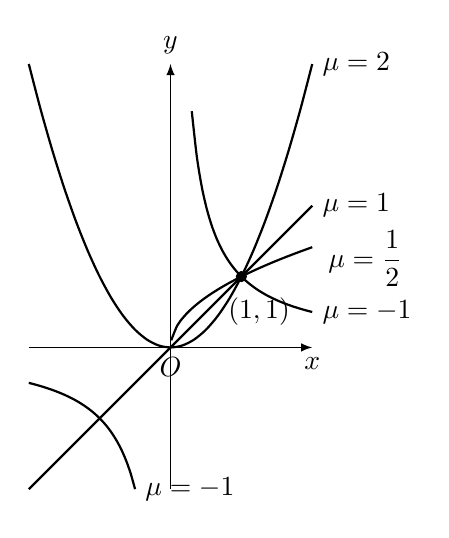
\begin{tikzpicture}[scale=0.9]
                \draw[-latex](-2,0) -- (2,0) node[below]{$x$};
                \draw[-latex](0,-2) -- (0,4) node[above]{$y$};
                \draw[black, thick, smooth, domain=0.3:2] plot (\x,1/\x) node[right]{$\mu =-1$};
                \draw[black, thick, smooth, domain=-2:-0.5] plot (\x,1/\x) node[right]{$\mu =-1$};
                \draw[black, thick, smooth, domain=0.01:2] plot (\x, {sqrt(\x)});
                \filldraw[black] (2.75,1.25) node {$\mu =\dfrac{1}{2}$};
                \draw[black, thick, smooth, domain=-2:2] plot (\x,\x) node[right]{$\mu =1$};
                \draw[black, thick, smooth, domain=-2:2] plot (\x, {\x*\x}) node[right]{$\mu =2$};
                \filldraw[black] (0,0) node[below]{$O$};
                \filldraw[black] (1,1) circle (2pt) node at(1.25,0.5){$(1,1)$};
            \end{tikzpicture}
        \end{minipage}
        \hfill
        \begin{minipage}{0.5\linewidth}
            对于幂函数可以根据不同幂下相同单调性来研究最值:

            \begin{enumerate}
                \item $\sqrt{u},\sqrt[3]{u}$可以使用$u$来研究。
                \item $\vert u\vert$可以使用$u^2$来研究。
                \item $\dfrac{1}{u},u>0$可以使用$u$来研究,但是最值相反。
                \item $u_1u_2...u_n$可以使用$\sum_{i=1}^{n}\ln u_i$来研究。
            \end{enumerate}
        \end{minipage}

        \subparagraph{指数函数} \leavevmode \medskip

        \begin{minipage}{0.4\linewidth}
            $y=a^x(a>0,a\neq 1)$:

            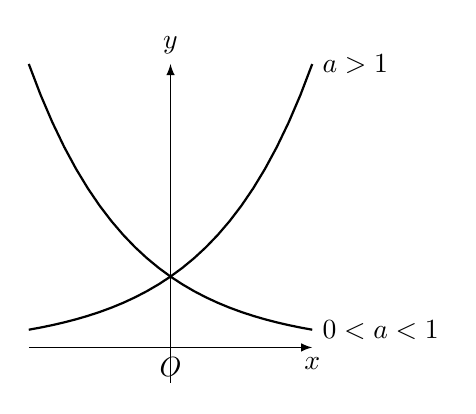
\begin{tikzpicture}[scale=0.9]
                \draw[-latex](-2,0) -- (2,0) node[below]{$x$};
                \draw[-latex](0,-0.5) -- (0,4) node[above]{$y$};
                \draw[black, thick, domain=-2:2] plot (\x,{pow(1/2,\x)}) node[right]{$0<a<1$};
                \draw[black, thick, domain=-2:2] plot (\x,{pow(2,\x)}) node[right]{$a>1$};
                \filldraw[black] (0,0) node[below]{$O$};
            \end{tikzpicture}
        \end{minipage}
        \hfill
        \begin{minipage}{0.5\linewidth}
            指数函数具有如下性质:

            \begin{enumerate}
                \item 特殊函数值:$a^0=1$。
                \item 定义域:$(-\infty, +\infty)$,值域:$(0,+\infty)$。
                \item 单调性:$a>1$,$y=a^x$单调增,$0<a<1$,$y=a^x$单调减。
                \item 常用指数函数:$y=e^x$。
                \item 极限:$\lim\limits_{x\to -\infty}e^x=0$,$\lim\limits_{x\to +\infty}e^x=+\infty$。
            \end{enumerate}
        \end{minipage}

        \subparagraph{对数函数} \leavevmode \medskip

        \begin{minipage}{0.45\linewidth}
            $y=log_ax(a>0,a\neq 1)$为$y=a^x$的反函数:

            常用公式:$x=e^{\ln x}$,$u^v=e^{\ln u^v}=e^{v\ln u}(x>0,u>0)$。
        \end{minipage}
        \hfill
        \begin{minipage}{0.45\linewidth}
            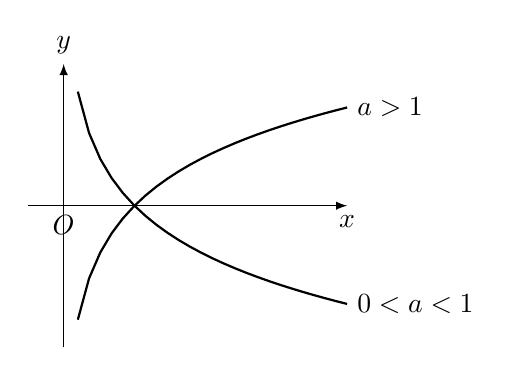
\begin{tikzpicture}[scale=0.9]
                \draw[-latex](-0.5,0) -- (4,0) node[below]{$x$};
                \draw[-latex](0,-2) -- (0,2) node[above]{$y$};
                \draw[black, thick, domain=0.2:4] plot (\x,{ln(1/\x)}) node[right]{$0<a<1$};
                \draw[black, thick, domain=0.2:4] plot (\x,{ln(\x)}) node[right]{$a>1$};
                \filldraw[black] (0,0) node[below]{$O$};
            \end{tikzpicture}
        \end{minipage}

        对数函数具有如下性质:

        \begin{enumerate}
            \item 特殊函数值:$\log_a1=0$,$log_aa=1,\ln 1=0,\ln e=1$。
            \item 定义域:$(0, +\infty)$,值域:$(-\infty,+\infty)$。
            \item 单调性:$a>1$,$y=\log_ax$单调增,$0<a<1$,$y=\log_ax$单调减。
            \item 常用对数函数:$y=\ln x$,$e=2.71828...$。
            \item 极限:$\lim\limits_{x\to 0^+}\log_a x=-\infty$,$\lim\limits_{x\to +\infty}\log_ax=+\infty$。
        \end{enumerate}


        \subparagraph{三角函数} \leavevmode \medskip

        正弦函数:

        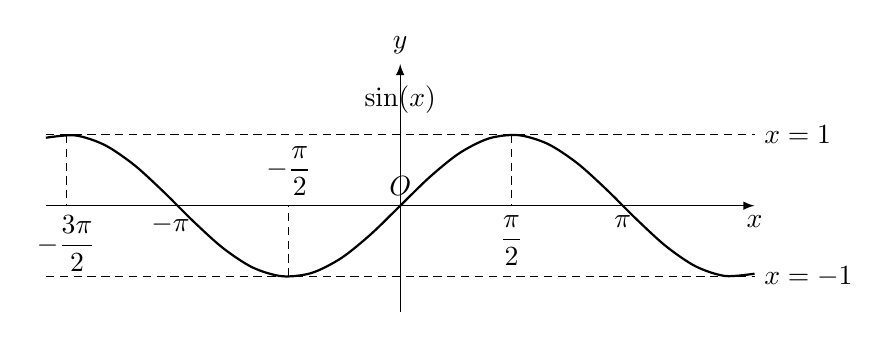
\begin{tikzpicture}[scale=0.9]
            \draw[-latex](-5,0) -- (5,0) node[below]{$x$};
            \draw[-latex](0,-1.5) -- (0,2) node[above]{$y$};
            \draw[black, thick, smooth, domain=-5:5] plot (\x,{sin(\x r)}) node at (0,1.5){$\sin(x)$};
            \draw[black, densely dashed](-5,1) -- (5,1) node[right]{$x=1$};
            \draw[black, densely dashed](-5,-1) -- (5,-1) node[right]{$x=-1$};
            \draw[black, densely dashed](-pi/2*3,1) -- (-pi/2*3,0) node[below]{$-\dfrac{3\pi}{2}$};
            \draw[black, densely dashed](-pi/2,-1) -- (-pi/2,0) node[above]{$-\dfrac{\pi}{2}$};
            \draw[black, densely dashed](pi/2,1) -- (pi/2,0) node[below]{$\dfrac{\pi}{2}$};
            \draw[black](0,0) -- (0,0) node[above]{$O$};
            \filldraw[black] (-pi-0.1,0) node[below]{$-\pi$};
            \filldraw[black] (pi,0) node[below]{$\pi$};
        \end{tikzpicture}

        余弦函数:

        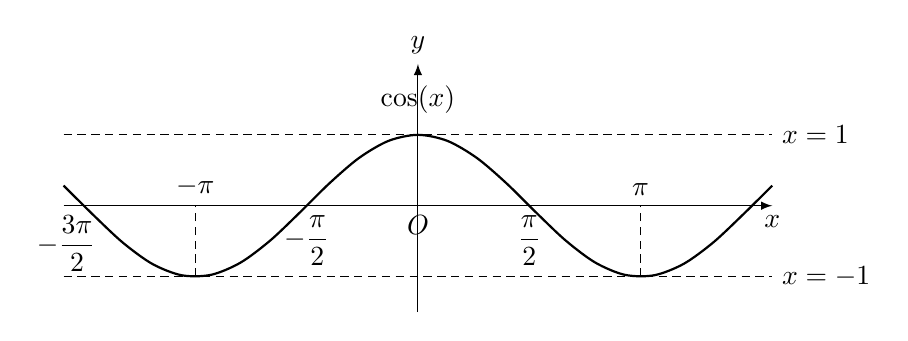
\begin{tikzpicture}[scale=0.9]
            \draw[-latex](-5,0) -- (5,0) node[below]{$x$};
            \draw[-latex](0,-1.5) -- (0,2) node[above]{$y$};
            \draw[black, thick, smooth, domain=-5:5] plot (\x,{cos(\x r)}) node at (0,1.5){$\cos(x)$};
            \draw[black, densely dashed](-5,1) -- (5,1) node[right]{$x=1$};
            \draw[black, densely dashed](-5,-1) -- (5,-1) node[right]{$x=-1$};
            \draw[black, densely dashed](-pi,-1) -- (-pi,0) node[above]{$-\pi$};
            \draw[black, densely dashed](pi,-1) -- (pi,0) node[above]{$\pi$};
            \filldraw[black] (0,0) node[below]{$O$};
            \filldraw[black] (-pi/2*3-0.25,0) node[below]{$-\dfrac{3\pi}{2}$};
            \filldraw[black] (-pi/2,0) node[below]{$-\dfrac{\pi}{2}$};
            \filldraw[black] (pi/2,0) node[below]{$\dfrac{\pi}{2}$};
        \end{tikzpicture}

        弦函数有如下特征:

        \begin{enumerate}
            \item 特殊函数值:$\sin 0=0$,$\sin\dfrac{\pi}{6}=\dfrac{1}{2}$,$\sin\dfrac{\pi}{4}=\dfrac{\sqrt{2}}{2}$,$\sin\dfrac{\pi}{3}=\dfrac{\sqrt{3}}{2}$,$\sin\dfrac{\pi}{2}=1$,$\sin\pi=0$,$\sin\dfrac{3\pi}{2}=-1$,$\sin 2\pi=0$,$\cos 0=1$,$\cos\dfrac{\pi}{6}=\dfrac{\sqrt{3}}{2}$,$\cos\dfrac{\pi}{4}=\dfrac{\sqrt{2}}{2}$,$\cos\dfrac{\pi}{3}=\dfrac{1}{2}$,$\cos\dfrac{\pi}{2}=0$,$\cos\pi=-1$,$\cos\dfrac{3\pi}{2}=0$,$\cos 2\pi=1$。
            \item 定义域:$(-\infty, +\infty)$,值域:$[-1,+1]$。
            \item 奇偶性:$y=\sin x$为奇函数,$y=\cos x$为偶函数。
            \item 周期性:最小正周期为$2\pi$。
            \item 有界性:$\vert\sin x\vert\leqslant 1$,$\vert\cos x\vert\leqslant 1$。
        \end{enumerate}

        \begin{minipage}{0.5\linewidth}
            正切函数:

            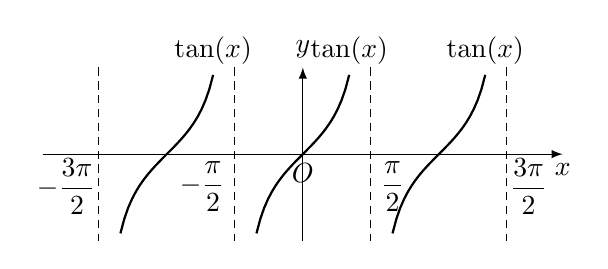
\begin{tikzpicture}[scale=0.55]
                \draw[-latex](-6,0) -- (6,0) node[below]{$x$};
                \draw[-latex](0,-2) -- (0,2) node[above]{$y$};
                \draw[black, thick, domain=-pi/2+0.5:pi/2-0.5] plot (\x,{tan(\x r)}) node[above]{$\tan(x)$};
                \draw[black, densely dashed](pi/2,2) -- (pi/2,-2);
                \draw[black, densely dashed](-pi/2,2) -- (-pi/2,-2);
                \draw[black, thick, domain=-pi/2*3+0.5:-pi/2-0.5] plot (\x,{tan(\x r)}) node[above]{$\tan(x)$};
                \draw[black, densely dashed](pi/2*3,2) -- (pi/2*3,-2);
                \draw[black, thick, domain=pi/2+0.5:pi/2*3-0.5] plot (\x,{tan(\x r)}) node[above]{$\tan(x)$};
                \draw[black, densely dashed](-pi/2*3,2) -- (-pi/2*3,-2);
                \filldraw[black] (0,0) node[below]{$O$};
                \filldraw[black] (pi/2+0.5,-0.75) node{$\dfrac{\pi}{2}$};
                \filldraw[black] (-pi/2-0.75,-0.75) node{$-\dfrac{\pi}{2}$};
                \filldraw[black] (pi/2*3+0.5,-0.75) node{$\dfrac{3\pi}{2}$};
                \filldraw[black] (-pi/2*3-0.75,-0.75) node{$-\dfrac{3\pi}{2}$};
            \end{tikzpicture}
        \end{minipage}
        \hfill
        \begin{minipage}{0.4\linewidth}
            余切函数:

            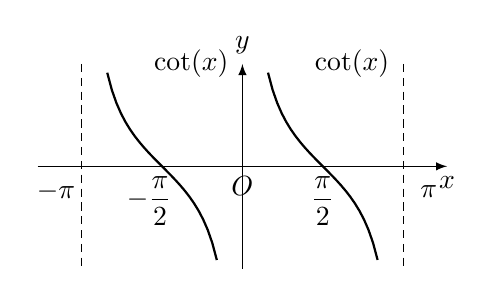
\begin{tikzpicture}[scale=0.65]
                \draw[-latex](-4,0) -- (4,0) node[below]{$x$};
                \draw[-latex](0,-2) -- (0,2) node[above]{$y$};
                \draw[black, thick, domain=0.5:pi-0.5] plot (\x,{cot(\x r)}) node at(pi-1,2){$\cot(x)$};
                \draw[black, densely dashed](pi,2) -- (pi,-2);
                \draw[black, thick, domain=-0.5:-pi+0.5] plot (\x,{cot(\x r)}) node at(-1,2){$\cot(x)$};
                \draw[black, densely dashed](-pi,2) -- (-pi,-2);
                \filldraw[black] (0,0) node[below]{$O$};
                \filldraw[black] (pi/2,0) node[below]{$\dfrac{\pi}{2}$};
                \filldraw[black] (pi+0.5,-0.5) node{$\pi$};
                \filldraw[black] (-pi/2-0.25,0) node[below]{$-\dfrac{\pi}{2}$};
                \filldraw[black] (-pi-0.5,-0.5) node{$-\pi$};
            \end{tikzpicture}
        \end{minipage}

        切函数有如下特征:

        \begin{enumerate}
            \item 特殊函数值:$\tan 0=0$,$\tan\frac{\pi}{6}=\frac{\sqrt{3}}{3}$,$\tan\frac{\pi}{4}=1$,$\tan\frac{\pi}{3}=\sqrt{3}$,$\lim\limits_{x\to\frac{\pi}{2}}\tan x=\infty$,$\tan\pi=0$,$\lim\limits_{x\to\frac{3\pi}{2}}\tan x=\infty$,$\tan 2\pi=0$,$\lim\limits_{x\to 0}\cot x=\infty$,$\cot\dfrac{\pi}{6}=\sqrt{3}$,$\cot\dfrac{\pi}{4}=1$,$\cot\dfrac{\pi}{3}=\dfrac{\sqrt{3}}{3}$,$\cot\dfrac{\pi}{2}=0$,$\lim\limits_{x\to\pi}\cot x=\infty$,$\cot\dfrac{3\pi}{2}=0$,$\lim\limits_{x\to 2\pi}\cot x=\infty$。
            \item 定义域:$\tan x:x\neq k\pi+\dfrac{\pi}{2}(k\in Z)$,$\cot x:x\neq k\pi(k\in Z)$,值域:$(-\infty,+\infty)$。
            \item 奇偶性:定义域内均为奇函数。
            \item 周期性:最小正周期为$\pi$。
        \end{enumerate}

        $\sec x=\dfrac{1}{\cos x},\csc x=\dfrac{1}{\sin x}$:

        正割函数:

        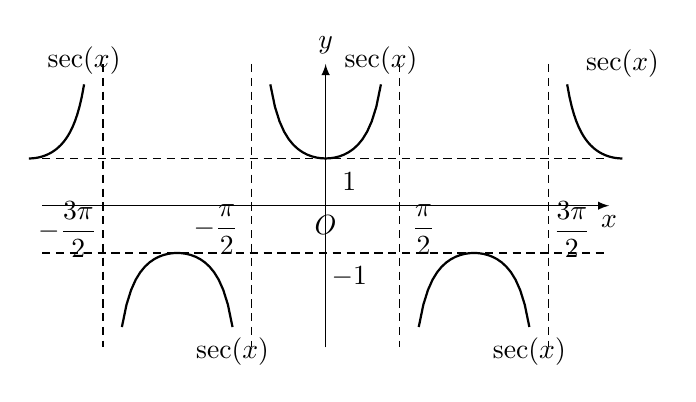
\begin{tikzpicture}[scale=0.6]
            \draw[-latex](-6,0) -- (6,0) node[below]{$x$};
            \draw[-latex](0,-3) -- (0,3) node[above]{$y$};
            \draw[black, thick, domain=-pi/2+0.4:pi/2-0.4] plot (\x,{sec(\x r)}) node[above]{$\sec(x)$};
            \draw[black, thick, domain=-pi/2*3+0.4:-pi/2-0.4] plot (\x,{sec(\x r)}) node[below]{$\sec(x)$};
            \draw[black, thick, domain=pi/2+0.4:pi/2*3-0.4] plot (\x,{sec(\x r)}) node[below]{$\sec(x)$};
            \draw[black, thick, domain=-pi*2:-pi/2*3-0.4] plot (\x,{sec(\x r)}) node[above]{$\sec(x)$};
            \draw[black, thick, domain=pi/2*3+0.4:pi*2] plot (\x,{sec(\x r)}) node at (pi*2,3){$\sec(x)$};
            \draw[black, densely dashed](-6,1) -- (6,1);
            \draw[black, densely dashed](-6,-1) -- (6,-1);
            \draw[black, densely dashed](-pi/2*3,3) -- (-pi/2*3,-3);
            \draw[black, densely dashed](-pi/2,3) -- (-pi/2,-3);
            \draw[black, densely dashed](pi/2,3) -- (pi/2,-3);
            \draw[black, densely dashed](pi/2*3,3) -- (pi/2*3,-3);
            \filldraw[black] (0,0) node[below]{$O$};
            \filldraw[black] (0.5,0.5) node{$1$};
            \filldraw[black] (0.5,-1.5) node{$-1$};
            \filldraw[black] (-pi/2*3-0.75,-0.5) node{$-\dfrac{3\pi}{2}$};
            \filldraw[black] (-pi/2-0.75,-0.5) node{$-\dfrac{\pi}{2}$};
            \filldraw[black] (pi/2+0.5,-0.5) node{$\dfrac{\pi}{2}$};
            \filldraw[black] (pi/2*3+0.5,-0.5) node{$\dfrac{3\pi}{2}$};
        \end{tikzpicture}

        余割函数:

        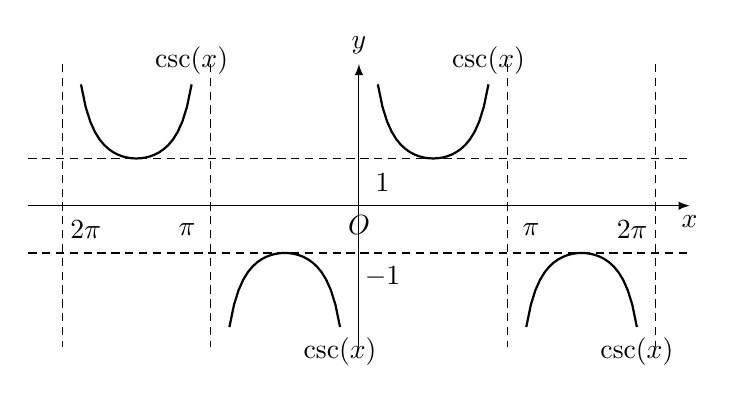
\begin{tikzpicture}[scale=0.6]
            \draw[-latex](-7,0) -- (7,0) node[below]{$x$};
            \draw[-latex](0,-3) -- (0,3) node[above]{$y$};
            \draw[black, thick, domain=0.4:pi-0.4] plot (\x,{1/sin(\x r)}) node[above]{$\csc(x)$};
            \draw[black, thick, domain=pi+0.4:pi*2-0.4] plot (\x,{1/sin(\x r)}) node[below]{$\csc(x)$};
            \draw[black, thick, domain=-pi+0.4:-0.4] plot (\x,{1/sin(\x r)}) node[below]{$\csc(x)$};
            \draw[black, thick, domain=-pi*2+0.4:-pi-0.4] plot (\x,{1/sin(\x r)}) node[above]{$\csc(x)$};
            \draw[black, densely dashed](-7,1) -- (7,1);
            \draw[black, densely dashed](-7,-1) -- (7,-1);
            \draw[black, densely dashed](-pi,3) -- (-pi,-3);
            \draw[black, densely dashed](-pi*2,3) -- (-pi*2,-3);
            \draw[black, densely dashed](pi,3) -- (pi,-3);
            \draw[black, densely dashed](pi*2,3) -- (pi*2,-3);
            \filldraw[black] (0,0) node[below]{$O$};
            \filldraw[black] (0.5,0.5) node{$1$};
            \filldraw[black] (0.5,-1.5) node{$-1$};
            \filldraw[black] (-pi-0.5,-0.5) node{$\pi$};
            \filldraw[black] (-pi*2+0.5,-0.5) node{$2\pi$};
            \filldraw[black] (pi+0.5,-0.5) node{$\pi$};
            \filldraw[black] (pi*2-0.5,-0.5) node{$2\pi$};
        \end{tikzpicture}

        割函数有如下特征:

        \begin{enumerate}
            \item 定义域:$\sec x:x\neq k\pi+\dfrac{\pi}{2}(k\in Z)$,$\csc x:x\neq k\pi(k\in Z)$,值域:$(-\infty,-1]\cup [1,+\infty)$。
            \item 奇偶性:$y=\sec x$为偶函数,$y=\csc x$为奇函数。
            \item 周期性:最小正周期为$2\pi$。
        \end{enumerate}

        \subparagraph{反三角函数} \leavevmode \medskip

        类似是三角函数的反函数,但是由于是个多值函数所以不是严格的函数。所以为了限制反三角函数为单值函数,将反三角函数的值限定在一个区间内,将其作为反三角函数的主值。

        \begin{minipage}{0.45\linewidth}
            反正弦函数:

            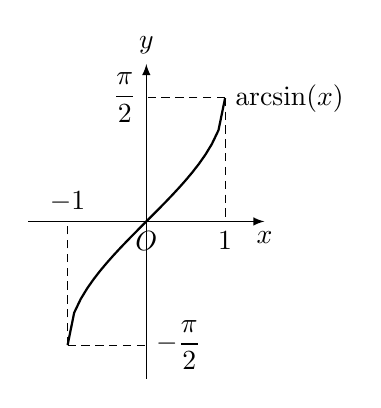
\begin{tikzpicture}
                \draw[-latex](-1.5,0) -- (1.5,0) node[below]{$x$};
                \draw[-latex](0,-2) -- (0,2) node[above]{$y$};
                \draw[black, thick, domain=-1:1] plot (\x,{rad(asin(\x))}) node[right]{$\arcsin(x)$};
                \draw[black, densely dashed](1,pi/2) -- (0,pi/2) node[left]{$\dfrac{\pi}{2}$};
                \filldraw[black] (0,0) node[below]{$O$};
                \draw[black, densely dashed](1,pi/2) -- (1,0) node[below]{$1$};
                \draw[black, densely dashed](-1,-pi/2) -- (0,-pi/2) node[right]{$-\dfrac{\pi}{2}$};
                \draw[black, densely dashed](-1,-pi/2) -- (-1,0) node[above]{$-1$};
            \end{tikzpicture}
        \end{minipage}
        \hfill
        \begin{minipage}{0.45\linewidth}
            反余弦函数:

            \begin{tikzpicture}
                \draw[-latex](-1.5,0) -- (1.5,0) node[below]{$x$};
                \draw[-latex](0,-0.5) -- (0,4) node[above]{$y$};
                \draw[black, thick, domain=-1:1] plot (\x,{rad(acos(\x)}) node at (-2, pi){$\arccos(x)$};
                \filldraw[black] (0,pi/2+0.5) node[right]{$\dfrac{\pi}{2}$};
                \draw[black](1,0) -- (1,0) node[below]{$1$};
                \filldraw[black] (0,0) node[below]{$O$};
                \draw[black, densely dashed](-1,pi) -- (0,pi) node[right]{$\pi$};
                \draw[black, densely dashed](-1,pi) -- (-1,0) node[below]{$-1$};
            \end{tikzpicture}
        \end{minipage}

        反弦函数有如下特征:

        \begin{enumerate}
            \item 特殊函数值:$\arcsin 0=0$,$\arcsin\dfrac{1}{2}=\dfrac{\pi}{6}$,$\arcsin\dfrac{\sqrt{2}}{2}=\dfrac{\pi}{4}$,$\arcsin\dfrac{\sqrt{3}}{2}=\dfrac{\pi}{3}$,$\arcsin 1=\dfrac{\pi}{2}$,$\arccos 1=0$,$\arccos\dfrac{\sqrt{3}}{2}=\dfrac{\pi}{6}$,$\arccos\dfrac{\sqrt{2}}{2}=\dfrac{\pi}{4}$,$\arccos\dfrac{1}{2}=\dfrac{\pi}{3}$,$\arccos 0=\dfrac{\pi}{2}$。
            \item 定义域:$(-1, +1)$,值域:$\arcsin x:[-\dfrac{\pi}{2},+\dfrac{\pi}{2}]$,$\arccos x:[0,\pi]$。
            \item 单调性:$y=\arcsin x$单调增,$y=\arccos x$单调减。
            \item 奇偶性:$y=\arcsin x$为奇函数。
            \item 有界性:$\vert\arcsin x\vert\leqslant\dfrac{\pi}{2}$,$0\leqslant\arccos x\leqslant\pi$。
            \item 性质:$\arcsin x+\arccos x=\dfrac{\pi}{2}(-1\leqslant x\leqslant 1)$
        \end{enumerate}

        对反弦函数性质进行证明:

        令$f(x)=\arcsin x+\arccos x$,对其求导得:$f'(x)=\dfrac{1}{\sqrt{1-x^2}}-\dfrac{1}{1-x^2}=0$,所以$f(x)$是个常数函数。

        又$f(0)=\dfrac{\pi}{2}$,所以该函数等于$\dfrac{\pi}{2}$。

        \begin{minipage}{0.45\linewidth}
            反正切函数:

            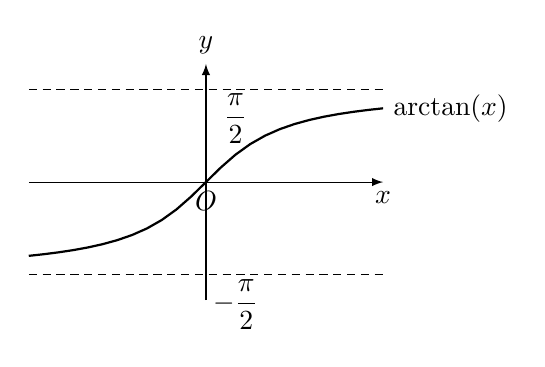
\begin{tikzpicture}[scale=0.75]
                \draw[-latex](-3,0) -- (3,0) node[below]{$x$};
                \draw[-latex](0,-2) -- (0,2) node[above]{$y$};
                \draw[black, thick, domain=-3:3] plot (\x,{rad(atan(\x))}) node[right]{$\arctan(x)$};
                \filldraw[black] (0,0) node[below]{$O$};
                \draw[black, densely dashed](-3,pi/2) -- (3,pi/2);
                \draw[black, densely dashed](-3,-pi/2) -- (3,-pi/2);
                \filldraw[black] (0.5,pi/2-0.5) node{$\dfrac{\pi}{2}$};
                \filldraw[black] (0.5,-pi/2-0.5) node{$-\dfrac{\pi}{2}$};
            \end{tikzpicture}
        \end{minipage}
        \hfill
        \begin{minipage}{0.45\linewidth}
            反余切函数:

            \begin{tikzpicture}[scale=0.75]
                \draw[-latex](-3,0) -- (3,0) node[below]{$x$};
                \draw[-latex](0,-0.5) -- (0,4) node[above]{$y$};
                \draw[black, thick, domain=-3:3] plot (\x,{pi/2-rad(atan(\x))}) node[right]{$\textrm{arccot}(x)$};
                \filldraw[black] (0,0) node[below]{$O$};
                \draw[black, densely dashed](-3,pi) -- (3,pi);
                \filldraw[black] (-0.5,pi/2-0.5) node{$\dfrac{\pi}{2}$};
            \end{tikzpicture}
        \end{minipage}

        反切函数有如下特征:

        \begin{enumerate}
            \item 特殊函数值:$\arctan 0=0$,$\arctan\dfrac{\pi}{6}=\dfrac{\sqrt{3}}{3}=$,$\arctan 1=\dfrac{\pi}{4}$,$\arctan\sqrt{3}=\dfrac{\pi}{3}$,$\textrm{arccot}\,0=\dfrac{\pi}{2}$,$\textrm{arccot}\,\sqrt{3}=\dfrac{\pi}{6}$,$\textrm{arccot}\,1=\dfrac{\pi}{4}$,$\textrm{arccot}\,\dfrac{\sqrt{3}}{3}=\dfrac{\pi}{3}$。
            \item 定义域:$(-\infty, +\infty)$,值域:$\arctan x:\left[-\dfrac{\pi}{2},+\dfrac{\pi}{2}\right]$,$\textrm{arccot}\,x:[0,\pi]$。
            \item 单调性:$y=\arctan x$单调增,$y=\textrm{arccot}\,x$单调减。
            \item 奇偶性:$y=\arctan x$为奇函数。
            \item 有界性:$\vert\arctan x\vert\leqslant\dfrac{\pi}{2}$,$0\leqslant\textrm{arccot}\,x\leqslant\pi$。
            \item 性质:$\arctan x+\textrm{arccot}\,x=\dfrac{\pi}{2}(-\infty<x<+\infty)$;$\arctan x=\textrm{arccot}\,x\dfrac{1}{x}=\dfrac{\pi}{2}-\arctan x$。
        \end{enumerate}

        \subparagraph{初等函数} \leavevmode \medskip

        由基本初等函数经过有限次四则运算与符合步骤且可以被一个式子所表示。

        幂指函数$u(x)^{v(x)}=e^{v(x)\ln u(x)}$也是初等函数。

        \paragraph{分段函数} \leavevmode \medskip

        x的不同范围对应不同的法则,经典形式如下:

        \begin{equation}\notag
        f(x)=\left\{ \begin{array}{lcl}
                         \psi_1(x), &  & x>x_0 \\
                         a,         &  & x=x_0 \\
                         \psi_2(x), &  & x<x_0
        \end{array}
        \right.
        \text{或}f(x)=\left\{ \begin{array}{clc}
                                  \psi(x), &  & x\neq x_0 \\
                                  a,       &  & x=x_0
        \end{array}
        \right.
        \end{equation}

        \subparagraph{绝对值函数} \leavevmode \medskip

        \begin{minipage}{0.45\linewidth}
            $
            y=\vert x\vert=\left\{
            \begin{array}{lcl}
                x,  &  & x\geqslant 0 \\
                -x, &  & x<0
            \end{array}
            \right.
            $
        \end{minipage}
        \hfill
        \begin{minipage}{0.45\linewidth}
            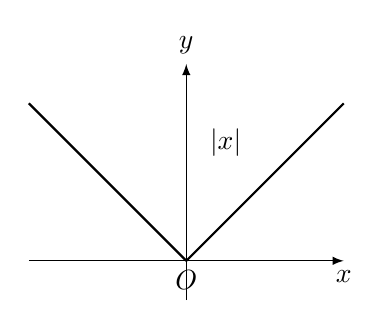
\begin{tikzpicture}
                \draw[-latex](-2,0) -- (2,0) node[below]{$x$};
                \draw[-latex](0,-0.5) -- (0,2.5) node[above]{$y$};
                \draw[black, thick, domain=0:2] plot (\x,\x);
                \draw[black, thick, domain=-2:0] plot (\x,-\x);
                \filldraw[black] (0.5,1.5) node{$\vert x\vert$};
                \filldraw[black] (0,0) node[below]{$O$};
            \end{tikzpicture}
        \end{minipage}

        \subparagraph{符号函数} \leavevmode \medskip

        \begin{minipage}{0.45\linewidth}
            $
            y=\textrm{sgn}\,x=\left\{
            \begin{array}{lcl}
                1,  &  & x>0 \\
                0,  &  & x=0 \\
                -1, &  & x<0
            \end{array}
            \right.
            $
        \end{minipage}
        \hfill
        \begin{minipage}{0.45\linewidth}
            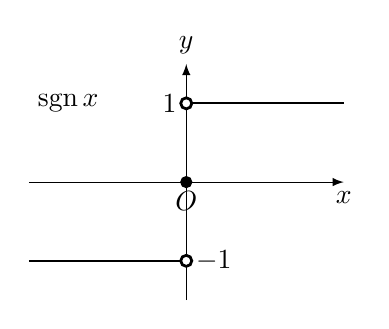
\begin{tikzpicture}
                \draw[-latex](-2,0) -- (2,0) node[below]{$x$};
                \draw[-latex](0,-1.5) -- (0,1.5) node[above]{$y$};
                \draw[black, thick, domain=0:2] plot (\x,1);
                \draw[black, thick, domain=-2:0] plot (\x,-1);
                \filldraw[black] (-1.5,1) node{$\textrm{sgn}\,x$};
                \filldraw[black] circle (2pt) (0,0) node[below]{$O$};
                \filldraw[white, draw=black, line width=1pt] (0,1) circle (2pt);
                \filldraw[black] (0,1) node[left]{$1$};
                \filldraw[white, draw=black, line width=1pt] (0,-1) circle (2pt);
                \filldraw[black] (0,-1) node[right]{$-1$};
            \end{tikzpicture}
        \end{minipage}

        \subparagraph{取整函数} \leavevmode \medskip

        $x$为实数,不超过$x$的最大整数称为其整数部分$[x]$,其定义域为$R$,值域为$Z$。

        \begin{minipage}{0.45\linewidth}
            \begin{enumerate}
                \item $x-1<[x]\leqslant x$。
                \item $\lim\limits_{x\to 0^+}[x]=0$。
                \item $\lim\limits_{x\to 0^-}[x]=-1$。
            \end{enumerate}
        \end{minipage}
        \hfill
        \begin{minipage}{0.45\linewidth}
            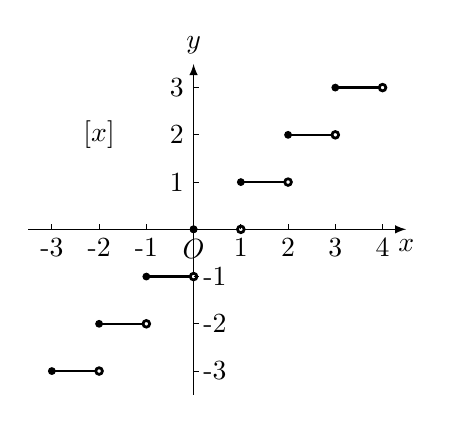
\begin{tikzpicture}[scale=0.6]
                \draw[-latex](-3.5,0) -- (4.5,0) node[below]{$x$};
                \draw[-latex](0,-3.5) -- (0,3.5) node[above]{$y$};
                \draw[black, thick, domain=1:2] plot (\x,1);
                \draw[black, thick, domain=2:3] plot (\x,2);
                \draw[black, thick, domain=3:4] plot (\x,3);
                \draw[black, thick, domain=-1:0] plot (\x,-1);
                \draw[black, thick, domain=-2:-1] plot (\x,-2);
                \draw[black, thick, domain=-3:-2] plot (\x,-3);
                \filldraw[black] (-2,2) node{$[x]$};
                \filldraw[black] circle (2pt) (0,0) node[below]{$O$};
                \foreach \x in {-2,...,4}
                \filldraw[white, draw=black, line width=1pt] (\x,\x-1) circle (2pt);
                \foreach \x in {3,...,-3}
                \filldraw[black] (\x,\x) circle (2pt);
                \foreach \x/\xtext in {-3,...,-1}
                \filldraw[black] (\x,0) node[below]{\xtext} -- ++(0, 3pt);
                \foreach \x/\xtext in {1,...,4}
                \filldraw[black] (\x,0) node[below]{\xtext} -- ++(0, 3pt);
                \foreach \x/\xtext in {1,...,3}
                \filldraw[black] (0,\x) node[left]{\xtext} -- +(3pt, 0);
                \foreach \x/\xtext in {-3,...,-1}
                \filldraw[black] (0,\x) node[right]{\xtext} -- +(3pt, 0);
            \end{tikzpicture}
        \end{minipage}

        \subsubsection{图像变换}
        \paragraph{平移变换}
        \subparagraph{左右平移} \leavevmode \medskip

        \begin{minipage}{0.35\linewidth}
            $f(x)$沿$x$轴左移$x_0$个单位长度得到$f(x+x_0)$,向右移动$x_0$个单位则得到$f(x-x_0)$:
        \end{minipage}
        \hfill
        \begin{minipage}{0.55\linewidth}
            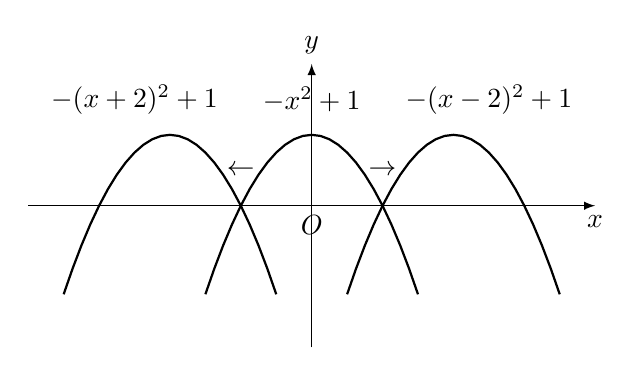
\begin{tikzpicture}[scale=0.9]
                \draw[-latex](-4,0) -- (4,0) node[below]{$x$};
                \draw[-latex](0,-2) -- (0,2) node[above]{$y$};
                \filldraw[black] (0,0) node[below]{$O$};
                \draw[black, thick, domain=-1.5:1.5] plot (\x,-\x*\x+1);
                \filldraw[black] (0,1.5) node{$-x^2+1$};
                \draw[black, thick, domain=0.5:3.5] plot (\x,{-pow((\x-2),2)+1});
                \filldraw[black] (2.5,1.5) node{$-(x-2)^2+1$};
                \draw[black, thick, domain=-3.5:-0.5] plot (\x,{-pow((\x+2),2)+1});
                \filldraw[black] (-2.5,1.5) node{$-(x+2)^2+1$};
                \filldraw[black] (1,0.5) node{$\rightarrow$};
                \filldraw[black] (-1,0.5) node{$\leftarrow$};
            \end{tikzpicture}
        \end{minipage}

        \subparagraph{上下平移} \leavevmode \medskip

        \begin{minipage}{0.45\linewidth}
            $f(x)$沿$y$轴上移$y_0$个单位长度得到$f(x)+y_0$,向下移动$y_0$个单位则得到$f(x)-y_0$:
        \end{minipage}
        \hfill
        \begin{minipage}{0.45\linewidth}
            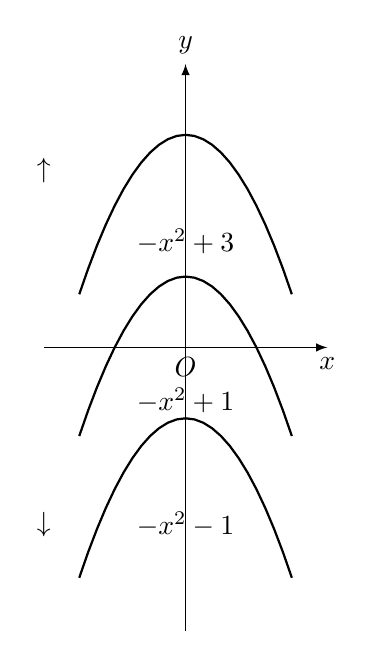
\begin{tikzpicture}[scale=0.9]
                \draw[-latex](-2,0) -- (2,0) node[below]{$x$};
                \draw[-latex](0,-4) -- (0,4) node[above]{$y$};
                \filldraw[black] (0,0) node[below]{$O$};
                \draw[black, thick, domain=-1.5:1.5] plot (\x,-\x*\x+1);
                \filldraw[black] (0,-0.75) node{$-x^2+1$};
                \draw[black, thick, domain=-1.5:1.5] plot (\x,{-\x*\x+3});
                \filldraw[black] (0,1.5) node{$-x^2+3$};
                \draw[black, thick, domain=-1.5:1.5] plot (\x,{-\x*\x+-1});
                \filldraw[black] (0,-2.5) node{$-x^2-1$};
                \filldraw[black] (-2,2.5) node{$\uparrow $};
                \filldraw[black] (-2,-2.5) node{$\downarrow $};
            \end{tikzpicture}
        \end{minipage}

        \paragraph{对称变换}
        \subparagraph{上下对称} \leavevmode \medskip

        \begin{minipage}{0.5\linewidth}
            将$f(x)$关于$x$轴对称得到$-f(x)$:
        \end{minipage}
        \hfill
        \begin{minipage}{0.4\linewidth}
            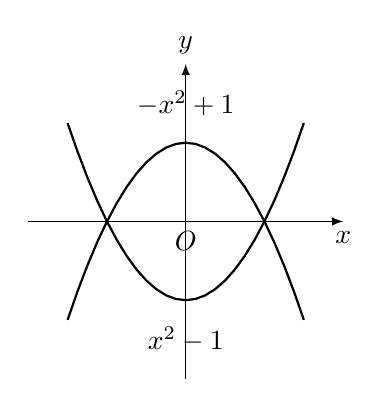
\begin{tikzpicture}
                \draw[-latex](-2,0) -- (2,0) node[below]{$x$};
                \draw[-latex](0,-2) -- (0,2) node[above]{$y$};
                \filldraw[black] (0,0) node[below]{$O$};
                \draw[black, thick, domain=-1.5:1.5] plot (\x,-\x*\x+1);
                \filldraw[black] (0,1.5) node{$-x^2+1$};
                \draw[black, thick, domain=-1.5:1.5] plot (\x,\x*\x-1);
                \filldraw[black] (0,-1.5) node{$x^2-1$};
            \end{tikzpicture}
        \end{minipage}

        \subparagraph{左右对称} \leavevmode \medskip

        \begin{minipage}{0.4\linewidth}
            将$f(x)$关于$y$轴对称得到\\$f(-x)$:
        \end{minipage}
        \hfill
        \begin{minipage}{0.5\linewidth}
            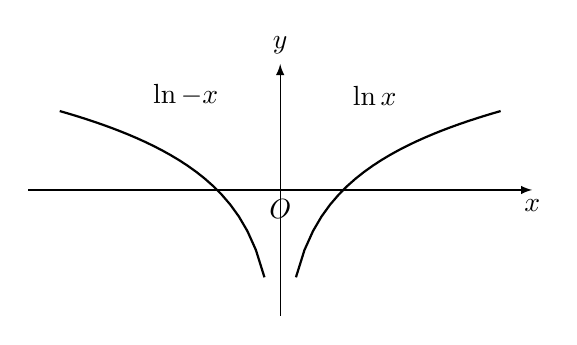
\begin{tikzpicture}[scale=0.8]
                \draw[-latex](-4,0) -- (4,0) node[below]{$x$};
                \draw[-latex](0,-2) -- (0,2) node[above]{$y$};
                \filldraw[black] (0,0) node[below]{$O$};
                \draw[black, thick, domain=0.25:3.5] plot (\x,{ln(\x)});
                \filldraw[black] (1.5,1.5) node{$\ln x$};
                \draw[black, thick, domain=-0.25:-3.5] plot (\x,{ln(-\x)});
                \filldraw[black] (-1.5,1.5) node{$\ln -x$};
            \end{tikzpicture}
        \end{minipage}

        \subparagraph{原点对称} \leavevmode \medskip

        \begin{minipage}{0.4\linewidth}
            将$f(x)$关于$x$轴$y$轴即关于原点对称得到$-f(-x)$:
        \end{minipage}
        \hfill
        \begin{minipage}{0.5\linewidth}
            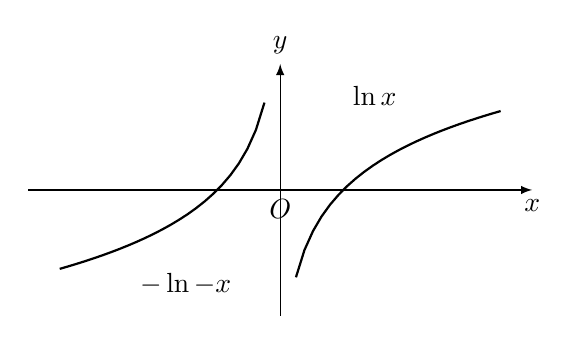
\begin{tikzpicture}[scale=0.8]
                \draw[-latex](-4,0) -- (4,0) node[below]{$x$};
                \draw[-latex](0,-2) -- (0,2) node[above]{$y$};
                \filldraw[black] (0,0) node[below]{$O$};
                \draw[black, thick, domain=0.25:3.5] plot (\x,{ln(\x)});
                \filldraw[black] (1.5,1.5) node{$\ln x$};
                \draw[black, thick, domain=-0.25:-3.5] plot (\x,{-ln(-\x)});
                \filldraw[black] (-1.5,-1.5) node{$-\ln -x$};
            \end{tikzpicture}
        \end{minipage}

        \subparagraph{反函数对称} \leavevmode \medskip

        \begin{minipage}{0.55\linewidth}
            将$f(x)$关于$y=x$轴对称得到$f^{-1}(x)$:
        \end{minipage}
        \hfill
        \begin{minipage}{0.35\linewidth}
            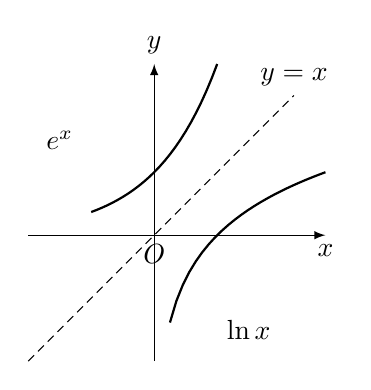
\begin{tikzpicture}[scale=0.8]
                \draw[-latex](-2,0) -- (e,0) node[below]{$x$};
                \draw[-latex](0,-2) -- (0,e) node[above]{$y$};
                \filldraw[black] (0,0) node[below]{$O$};
                \draw[black, thick, domain=0.25:e] plot (\x,{ln(\x)});
                \filldraw[black] (1.5,-1.5) node{$\ln x$};
                \draw[black, thick, domain=-1:1] plot (\x,{exp(\x)});
                \filldraw[black] (-1.5,1.5) node{$e^x$};
                \draw[black, densely dashed] (-2,-2) -- (e-0.5,e-0.5) node[above]{$y=x$};
            \end{tikzpicture}
        \end{minipage}

        \subparagraph{函数绝对值} \leavevmode \medskip

        \begin{minipage}{0.5\linewidth}
            保留$f(x)$函数值在$[0,\infty]$的部分,并对$[-\infty,0]$部分进行上下对称:
        \end{minipage}
        \hfill
        \begin{minipage}{0.4\linewidth}
            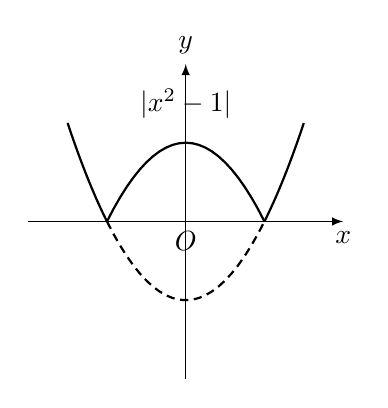
\begin{tikzpicture}
                \draw[-latex](-2,0) -- (2,0) node[below]{$x$};
                \draw[-latex](0,-2) -- (0,2) node[above]{$y$};
                \filldraw[black] (0,0) node[below]{$O$};
                \draw[black, thick, domain=1:1.5] plot (\x,\x*\x-1);
                \draw[black, thick, densely dashed, domain=-1:1] plot (\x,\x*\x-1);
                \draw[black, thick, domain=-1:1] plot (\x,-\x*\x+1);
                \draw[black, thick, domain=-1.5:-1] plot (\x,\x*\x-1);
                \filldraw[black] (0,1.5) node{$\vert x^2-1\vert$};
            \end{tikzpicture}
        \end{minipage}

        \subparagraph{自变量绝对值} \leavevmode \medskip

        \begin{minipage}{0.5\linewidth}
            先只保留$f(x)$定义域在$[0,\infty]$的部分,然后在$[-\infty,0]$部分使用$[0,\infty]$的部分进行左右对称:
        \end{minipage}
        \hfill
        \begin{minipage}{0.4\linewidth}
            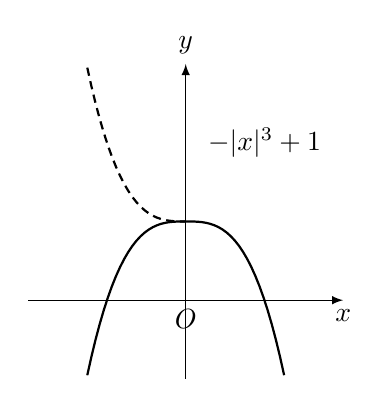
\begin{tikzpicture}
                \draw[-latex](-2,0) -- (2,0) node[below]{$x$};
                \draw[-latex](0,-1) -- (0,3) node[above]{$y$};
                \filldraw[black] (0,0) node[below]{$O$};
                \draw[black, thick, domain=0:1.25] plot (\x,{-pow(\x,3)+1});
                \draw[black, thick, densely dashed, domain=-1.25:0] plot (\x,{-pow(\x,3)+1});
                \draw[black, thick, domain=-1.25:0] plot (\x,{-pow(-\x,3)+1});
                \filldraw[black] (1,2) node{$-\vert x\vert^3+1$};
            \end{tikzpicture}
        \end{minipage}

        \paragraph{伸缩变换}
        \subparagraph{水平伸缩} \leavevmode \medskip

        \begin{minipage}{0.35\linewidth}
            纵坐标不变,当$k>1$时,$y=f(kx)$是$y=f(x)$缩短k倍得到,当$0<k<1$时,$y=f(kx)$是$y=f(x)$伸长k倍得到:
        \end{minipage}
        \hfill
        \begin{minipage}{0.55\linewidth}
            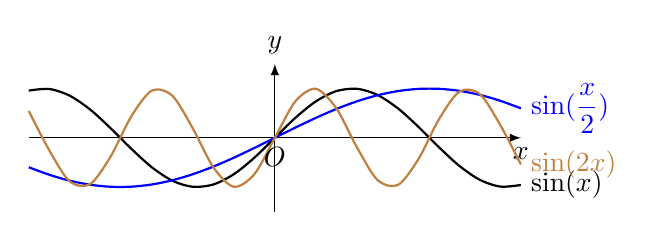
\begin{tikzpicture}[scale=0.625]
                \draw[-latex](-5,0) -- (5,0) node[below]{$x$};
                \draw[-latex](0,-1.5) -- (0,1.5) node[above]{$y$};
                \draw[black, thick, smooth, domain=-5:5] plot (\x,{sin(\x r)}) node[right]{$\sin(x)$};
                \draw[blue, thick, smooth, domain=-5:5] plot (\x,{sin(\x/2 r)}) node[right]{$\sin(\dfrac{x}{2})$};
                \draw[brown, thick, smooth, domain=-5:5] plot (\x,{sin(\x*2 r)}) node[right]{$\sin(2x)$};
                \filldraw[black] (0,0) node[below]{$O$};
            \end{tikzpicture}
        \end{minipage}

        \subparagraph{垂直伸缩} \leavevmode \medskip

        \begin{minipage}{0.35\linewidth}
            横坐标不变,$y=kf(x)$的对应纵坐标为$y=f(x)$对应纵坐标的$k$倍。
        \end{minipage}
        \hfill
        \begin{minipage}{0.55\linewidth}
            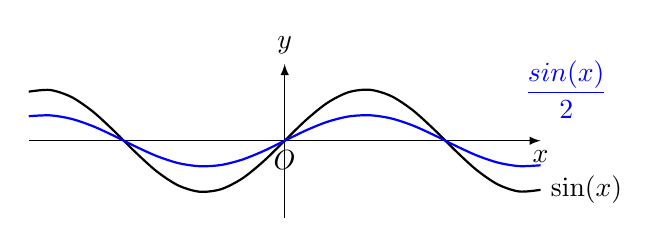
\begin{tikzpicture}[scale=0.65]
                \draw[-latex](-5,0) -- (5,0) node[below]{$x$};
                \draw[-latex](0,-1.5) -- (0,1.5) node[above]{$y$};
                \draw[black, thick, smooth, domain=-5:5] plot (\x,{sin(\x r)}) node[right]{$\sin(x)$};
                \draw[blue, thick, smooth, domain=-5:5] plot (\x,{sin(\x r)/2}) node at(5.5,1){$\dfrac{sin(x)}{2}$};
                \filldraw[black] (0,0) node[below]{$O$};
            \end{tikzpicture}
        \end{minipage}

        \subsection{极坐标系图像}
        \subsubsection{极坐标系}

        \paragraph{极坐标定义} \leavevmode \medskip

        \begin{itemize}
            \item 极点:平面内的一个定点$O$。
            \item 极轴:自极点引出的射线$Ox$。
            \item 极坐标系:选定长度单位、角度单位与正方向(通常为逆时针)建立的坐标系。
            \item 极径:设$M$为屏幕一点,极点$O$与$M$的距离$\vert OM\vert$,记为$\rho$。
            \item 极角:以极轴$Ox$为始边,射线$OM$为终边的角$xOM$为$M$的极角,记为$\theta$。
            \item 极坐标:有序数对$\rho$、$\theta$为$M$的极坐标,记为$M(\rho,\theta)$。
        \end{itemize}

        \paragraph{极坐标系转换} \leavevmode \medskip

        设$M$为平面一点,直角坐标为$(x,y)$,极坐标$(\rho,\theta)$,其关系是:\medskip

        $\left\{\begin{array}{l}
                    x=\rho\cos\theta \\
                    y=\rho\sin\theta
        \end{array}\right.$,$\left\{\begin{array}{l}
                                        \rho^2=x^2+y^2 \\
                                        \tan\theta=\dfrac{y}{x}(x\neq0)
        \end{array}\right.$\medskip

        \paragraph{常用极坐标方程} \leavevmode \medskip

        直线的极坐标方程:

        \begin{itemize}
            \item 从极点$O$发出的一条射线:$\tan\theta=k$(由于$k$不知道符号所以不能直接转换为反三角函数)。
            \item 过点$(a,0)$且垂直于极轴的直线的极坐标方程:$\rho=a\sec\theta=\dfrac{a}{\cos\theta}$。
            \item 过点$\left(a,\dfrac{\pi}{2}\right)$且平行于极轴的直线的极坐标方程:$\rho=a\csc\theta=\dfrac{a}{\sin\theta}$。
        \end{itemize}

        圆的极坐标方程:

        \begin{itemize}
            \item 圆心为极点,半径为$r$的圆的极坐标方程:$\rho=r$。
            \item 圆心$O'(r,0)$,半径为$r$的圆的极坐标方程:$\rho=2r\cos\theta$。
            \item 圆心$O'\left(r,\dfrac{\pi}{2}\right)$,半径为$r$的圆的极坐标方程:$\rho=2r\sin\theta$。
                    % \item 圆心$O'(\rho_0,0)$,半径为$r$的圆的极坐标方程:
        \end{itemize}

        抛物线的极坐标方程:

        \begin{itemize}
            \item $y=ax^2$的极坐标方程:$\rho=\dfrac{1}{a}\tan\theta\sec\theta$。
            \item $y^2=ax$的极坐标方程:$\rho=a\cot\theta\csc\theta$。
        \end{itemize}

        \subsubsection{描点法}
        \paragraph{心形线(外摆线)} \leavevmode \medskip

        \begin{minipage}{0.55\linewidth}
            心形线又称为心脏线,表示是一个圆上的固定一点在它绕着与其相切且半径相同的另外一个圆周滚动时所形成的轨迹。

            表达式:水平为$r=a(1\pm\cos\theta)$,垂直为$r=a(1\pm\sin\theta)$。一般为$r=a(1-\cos\theta)$即为下图所示,如果里面的符号为+则心尖开口向左。

            其中$r$为线的极径,$\theta$为极角,$a$为形状参数且$a>0$,周期为$2\pi$。
        \end{minipage}
        \hfill
        \begin{minipage}{0.35\linewidth}
            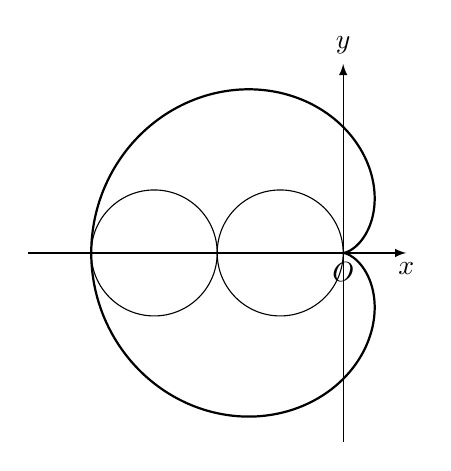
\begin{tikzpicture}[scale=0.8]
                \draw[-latex](-5,0) -- (1,0) node[below]{$x$};
                \draw[-latex](0,-3) -- (0,3) node[above]{$y$};
                \draw[black, thick, domain=0:360,smooth,variable=\t, samples=300] plot ({\t}:{2*(1-cos(\t))});
                \filldraw[black] (0,0) node[below]{$O$};
                \draw (-1,0) circle [radius=1];
                \draw (-3,0) circle [radius=1];
            \end{tikzpicture}
        \end{minipage}

        在直角坐标系下表达式:$x^2+y^2+a\cdot x=a\cdot\sqrt{x^2+y^2}$和$x^2+y^2-a\cdot x=a\cdot\sqrt{x^2+y^2}$。

        参数方程:$x=a\cdot(2\cdot\cos(t)-cos(2\cdot t))$与$y=a\cdot(2\cdot\sin(t)-sin(2\cdot t))$。

        水平心形线对应参数: \leavevmode \medskip

        \begin{tabular}{|c|c|c|c|c|c|c|c|c|c|}
            \hline
            $\theta$ & $0$ & $\dfrac{\pi}{6}$         & $\dfrac{\pi}{4}$         & $\dfrac{\pi}{3}$ & $\dfrac{\pi}{2}$ & $\dfrac{2\pi}{3}$ & $\dfrac{3\pi}{4}$        & $\dfrac{5\pi}{6}$        & $\pi$ \\ \hline
            $r$      & $0$ & $\dfrac{2-\sqrt{3}}{2}a$ & $\dfrac{2-\sqrt{2}}{2}a$ & $\dfrac{1}{2}a$  & $a$             & $\dfrac{3}{2}a$   & $\dfrac{2+\sqrt{2}}{2}a$ & $\dfrac{2+\sqrt{3}}{2}a$ & $2a$  \\
            \hline
        \end{tabular}

        \paragraph{玫瑰线} \leavevmode \medskip

        \begin{minipage}{0.55\linewidth}
            表达式:$r=a\sin(n\theta)$,周期为$\dfrac{2\pi}{n}$。

            当$n$为3时为三叶,2时为四叶,$\dfrac{3}{2}$为六叶。三叶时周期为$\dfrac{2\pi}{3}$。

            直角坐标系下表达式:$x=a\cdot\sin(n\cdot\theta)\cdot\cos(\theta)$与$y=a\cdot\sin(n\cdot)\cdot\sin(\theta)$
        \end{minipage}
        \hfill
        \begin{minipage}{0.35\linewidth}
            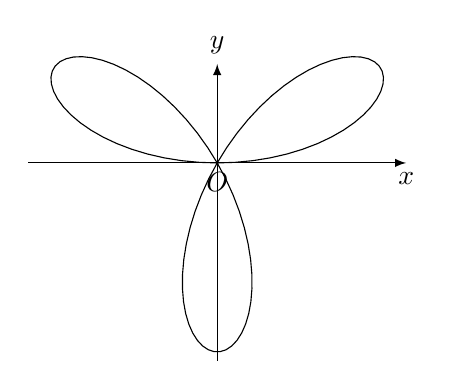
\begin{tikzpicture}[scale=0.8]
                \draw[-latex](-3,0) -- (3,0) node[below]{$x$};
                \draw[-latex](0,-pi) -- (0,pi/2) node[above]{$y$};
                \draw[domain=0:180,samples=100] plot (\x:{3*sin(\x*3)});
                \filldraw[black] (0,0) node[below]{$O$};
            \end{tikzpicture}
        \end{minipage}

        三叶玫瑰线对应参数: \leavevmode \medskip

        \begin{tabular}{|c|c|c|c|c|c|c|c|c|c|}
            \hline
            $\theta$ & $0$ & $\dfrac{\pi}{12}$      & $\dfrac{\pi}{6}$ & $\dfrac{\pi}{4}$       & $\dfrac{\pi}{3}$ & $\dfrac{5\pi}{12}$     & $\dfrac{\pi}{2}$ & $\dfrac{7\pi}{12}$     & $\dfrac{3\pi}{2}$ \\ \hline
            $r$      & $0$ & $\dfrac{\sqrt{2}}{2}a$ & $a$             & $\dfrac{\sqrt{2}}{2}a$ & $0$             & $-frac{\sqrt{2}}{2}a$ & $-a$            & $-frac{\sqrt{2}}{2}a$ & $0$              \\
            \hline
        \end{tabular}

        \paragraph{阿基米德螺线} \leavevmode \medskip

        \begin{minipage}{0.5\linewidth}
            表达式:$r=a\theta$,其中$a>0$,$\theta\geqslant 0$由0开始增大时$r$也在不断增大。
        \end{minipage}
        \hfill
        \begin{minipage}{0.4\linewidth}
            \begin{tikzpicture}[scale=0.2]
                \draw[-latex](-10,0) -- (15,0) node[below]{$x$};
                \draw[-latex](0,-15) -- (0,10) node[above]{$y$};
                \draw[domain=0:720,samples=100] plot (\x:{rad(\x)});
                \filldraw[black] (0,0) node[below]{$O$};
            \end{tikzpicture}
        \end{minipage}

        \paragraph{伯努利双扭线} \leavevmode \medskip

        设定线段$F_1F_2$长度为$2a$,伯努利双扭线上所有点M满足$MF_1\cdot MF_2=a^2$。

        表达式:$r^2=2a^2\cos 2\theta$或$r^2=2a^2\sin 2\theta$。

        直角坐标系下表达式:$(x^2+y^2)^2=2a^2(x^2-y^2)$。

        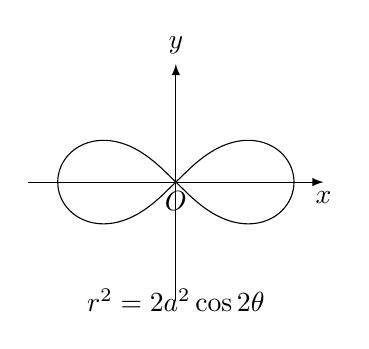
\begin{tikzpicture}[scale=1.5]
            \draw[-latex](-1.25,0) -- (1.25,0) node[below]{$x$};
            \draw[-latex](0,-1) -- (0,1) node[above]{$y$};
            \draw[domain=-45:45,samples=100] plot (\x:{sqrt(cos(\x*2))});
            \draw[domain=-45:45,samples=100] plot (\x:{-sqrt(cos(\x*2))});
            \filldraw[black] (0,0) node[below]{$O$};
            \filldraw[black] (0,-1) node{$r^2=2a^2\cos 2\theta$};
        \end{tikzpicture}
        \hspace{2.5em}
        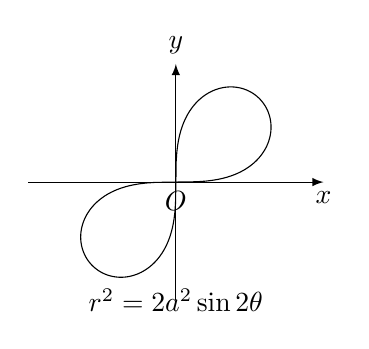
\begin{tikzpicture}[scale=1.5]
            \draw[-latex](-1.25,0) -- (1.25,0) node[below]{$x$};
            \draw[-latex](0,-1) -- (0,1) node[above]{$y$};
            \draw[domain=0:90,samples=100] plot (\x:{sqrt(sin(\x*2))});
            \draw[domain=0:90,samples=100] plot (\x:{-sqrt(sin(\x*2))});
            \filldraw[black] (0,0) node[below]{$O$};
            \filldraw[black] (0,-1) node{$r^2=2a^2\sin 2\theta$};
        \end{tikzpicture}

        \subsubsection{直角坐标系下画极坐标图像}

        \begin{minipage}{0.5\linewidth}
            令$\theta$为$x$,令$r$为$y$。如心形线$r=2(1-\cos\theta)$:

            按直角坐标系的图就可以计算出对应的$r$从而能画出对应的图像。
        \end{minipage}
        \hfill
        \begin{minipage}{0.4\linewidth}
            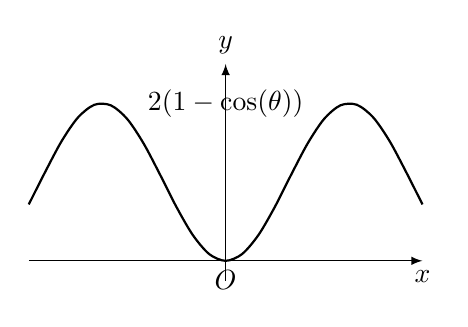
\begin{tikzpicture}[scale=0.5]
                \draw[-latex](-5,0) -- (5,0) node[below]{$x$};
                \draw[-latex](0,-0.5) -- (0,5) node[above]{$y$};
                \draw[black, thick, smooth, domain=-5:5] plot (\x,{2*(1-cos(\x r))}) node at (0,4){$2(1-\cos(\theta))$};
                \filldraw[black] (0,0) node[below]{$O$};
            \end{tikzpicture}
        \end{minipage}

        \subsection{参数法}

        如果很难使用直角坐标或极坐标来表示曲线,那么可以引入一个新的变量参数来表示,即得到参数方程:$
        \left\{
        \begin{array}{lcl}
            x=x(t) \\
            y=y(t)
        \end{array}
        \right.
        $

        \subsubsection{摆线(平摆线)}

        摆线,又称旋轮线、圆滚线,是一个圆沿一条直线滚动时,圆边界上一定点所形成的轨迹。

        令圆半径为$r$,摆点与圆心所成直线所转动夹角对应弧度为$t$,其中$t\in[0,2\pi]$,所对应参数方程为:$
        \left\{
        \begin{array}{lcl}
            x=r(t-\sin t) \\
            y=r(1-\cos t)
        \end{array}
        \right.
        $

        \begin{tikzpicture}[scale=1.5]
            \draw[-latex](-1.5,0) -- (5,0) node[below]{$x$};
            \draw[-latex](0,-0.5) -- (0,2) node[above]{$y$};
            \filldraw[black] (0,0) node[below]{$O$};
            \draw[black,scale=0.35, domain=-1.7:2*4.0, smooth, variable=\t ]
            plot ( {2*(\t-sin(\t r))}, {2*(1-cos(\t r))});
            \draw (0.7,0.7) circle [radius=0.7];
            \draw[black](0.7,0) -- (0.7,1.4);
            \draw[black, densely dashed](2.25,0) -- (2.25,1.4);
            \filldraw[black] (2.5,0.625) node{$2a$};
        \end{tikzpicture}

        \subsubsection{星形线(内摆线)}

        \begin{minipage}{0.5\linewidth}
            与半径为$r$的定圆内切的半径为$\dfrac{r}{4}$的动圆沿定圆无滑动地滚动,动圆上一点的轨迹称为星形线。

            令$t$表示摆点与圆心的连线所构成夹角的弧度,其中$t\in[0,2\pi]$,得对应参数方程:$
            \left\{
            \begin{array}{lcl}
                x=r\cos^3t \\
                y=r\sin^3t
            \end{array}
            \right.
            $

            由$\cos^2t+\sin^2t=1$得到直角坐标方程:$x^{\frac{2}{3}}+y^{\frac{2}{3}}=r^{\frac{2}{3}}$。
        \end{minipage}
        \hfill
        \begin{minipage}{0.4\linewidth}
            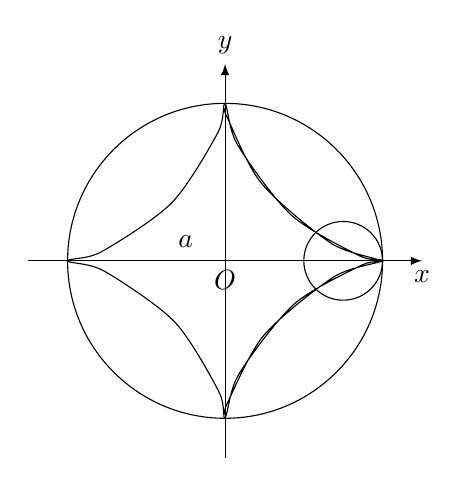
\begin{tikzpicture}[scale=2]
                \draw[-latex](-1.25,0) -- (1.25,0) node[below]{$x$};
                \draw[-latex](0,-1.25) -- (0,1.25) node[above]{$y$};
                \filldraw[black] (0,0) node[below]{$O$};
                \draw[black,scale=1, domain=-1.7:2*4.0, smooth, variable=\t ]
                plot ( {(pow(cos(\t r),3))}, {(pow(sin(\t r),3))});
                \filldraw[black] (-0.25,0.125) node{$a$};
                \draw (0,0) circle [radius=1];
                \draw (0.75,0) circle [radius=0.25];
            \end{tikzpicture}
        \end{minipage}

        \section{常用基础知识}
        \subsection{数列}
        \subsubsection{等差数列}

        首项为$a_1$,公差为$d(d\neq 0)$的数列:$a_1,a_1+d,a_1+2d\cdots a_1+(n-1)d$。

        通项公式:$a_n=a_1+(n-1)d$。

        前$n$项和:$S_n=\dfrac{n}{2}[2a_1+(n-1)d]=\dfrac{n}{2}(a_1+a_n)$

        \subsubsection{等比数列}

        首项为$a_1$,公比为$q(q\neq 0)$的数列:$a_1,a_1q,a_1a^2\cdots a_1q^{n-1}$。

        通项公式:$a_n=a_1q^{n-1}$。

        前$n$项和:$S_n=
        \left\{
        \begin{array}{lcl}
            na_1,                   &  & r=1     \\
            \dfrac{a_1(1-r^n)}{1-r}, &  & r\neq 1
        \end{array}
        \right.$

        若首项为1,则$1+r+r^2+\cdots+r^{n-1}=\dfrac{1-r^n}{1-r}(r\neq 1)$。

        则对无穷的极限为$\dfrac{1}{1-r}$。

        \subsubsection{常见数列前\texorpdfstring{$n$}n项和}

        \begin{enumerate}
            \item $\sum_{k=1}^nk=1+2+\cdots+n=\dfrac{n(n+1)}{2}$。
            \item $\sum_{k=1}^nk^2=1^2+2^2+\cdots+n^2=\dfrac{n(n+1)(2n+1)}{6}$。
            \item $\sum_{k=1}^n\dfrac{1}{k(k+1)}=\dfrac{1}{1\times 2}+\dfrac{1}{2\times 3}+\cdots+\dfrac{1}{n(n+1)}=\dfrac{n}{n+1}$。
        \end{enumerate}

        \subsection{三角函数}

        \subsubsection{基本关系}

        $\csc\alpha=\dfrac{1}{\sin\alpha},\sec\alpha=\dfrac{1}{\cos\alpha},\cot\alpha=\dfrac{1}{\tan\alpha},\tan\alpha=\dfrac{\sin\alpha}{\cos\alpha},\cot\alpha=\dfrac{\cos\alpha}{\sin\alpha}$。

        $\sin^2\alpha+\cos^2\alpha=1,1+\tan^2\alpha=\sec^2\alpha,1+\cot^2\alpha=\csc^2\alpha$。

        $\cos^2\alpha=1-\sin^2\alpha=(1+\sin\alpha)(1-\sin\alpha)$,$\sin^2\alpha=1-\cos^2\alpha=(1+\cos\alpha)(1-\cos\alpha)$。

        \subsubsection{诱导公式}

        奇变偶不变,符号看象限。奇指前面添加的常数项是否为$\pi$的整数倍,是就需要改变函数,看象限指添加了常数后整体的符号看函数所在象限的符号。

        \begin{enumerate}
            \item $\sin(\dfrac{\pi}{2}\pm\alpha)=\cos\alpha$
            \item $\cos(\dfrac{\pi}{2}\pm\alpha)=\mp\sin\alpha$
            \item $\sin(\pi\pm\alpha)=\mp\sin\alpha$
            \item $\cos(\pi\pm\alpha)=-\cos\alpha$
        \end{enumerate}

        \subsubsection{倍角公式}

        $\sin 2\alpha=2\sin\alpha\cos\alpha$,$\cos 2\alpha=\cos^2\alpha-\sin^2\alpha=(\sin\alpha+\cos\alpha)(\cos\alpha-\sin\alpha)=1-2\sin^2\alpha=2\cos^2\alpha-1$。

        $1+\sin2\alpha=(\sin\alpha+\cos\alpha)^2$,$1-\sin2\alpha=(\sin\alpha-\cos\alpha)^2$。

        $\sin 3\alpha=-4\sin^3\alpha_3\sin\alpha,\cos 3\alpha=4\cos^3\alpha-3\cos\alpha$。

        $\tan 2\alpha=\dfrac{2\tan\alpha}{1-\tan^2\alpha},\cot 2\alpha=\dfrac{\cot^2\alpha-1}{2\cot\alpha}$。

        \subsubsection{半角公式}

        $\sin^2\dfrac{\alpha}{2}=\dfrac{1}{2}(1-\cos\alpha),\cos^2\dfrac{\alpha}{2}=\dfrac{1}{2}(1+\cos\alpha)\text{(降幂公式)}$。

        $\sin\dfrac{\alpha}{2}=\pm\sqrt{\dfrac{1-\cos\alpha}{2}},\cos\dfrac{\alpha}{2}=\pm\sqrt{\dfrac{1+\cos\alpha}{2}}$。

        $\tan\dfrac{\alpha}{2}=\dfrac{1-\cos\alpha}{\sin\alpha}=\dfrac{\sin\alpha}{1+\cos\alpha}=\pm\sqrt{\dfrac{1-\cos\alpha}{1+\cos\alpha}}=\dfrac{1}{\cot\dfrac{\alpha}{2}}$。

        \subsubsection{和差公式}

        $\sin$和$\tan$的和差公式更容易考到。

        $\sin(\alpha\pm\beta)=\sin\alpha\cos\beta\pm\cos\alpha\sin\beta,\cos(\alpha\pm\beta)=\cos\alpha\cos\beta\mp\sin\alpha\sin\beta$。

        $\tan(\alpha\pm\beta)=\dfrac{\tan\alpha\pm\tan\beta}{1\mp\tan\alpha\tan\beta},\cot(\alpha\pm\beta)=\dfrac{\cot\alpha\cot\beta\mp 1}{\cot\beta\pm\cot\alpha}$。

        \subsubsection{积化和差公式}

        和差化积与积化和差不需要背,都是和差公式的推导。

        $\sin\alpha\cos\beta=\dfrac{1}{2}[\sin(\alpha+\beta)+\sin(\alpha-\beta)],\cos\alpha\sin\beta=\dfrac{1}{2}[\sin(\alpha+\beta)-\sin(\alpha-\beta)]$。

        $\cos\alpha\cos\beta=\dfrac{1}{2}[\cos(\alpha+\beta)+\cos(\alpha-\beta)],\sin\alpha\sin\beta=\dfrac{1}{2}[\cos(\alpha-\beta)-\cos(\alpha+\beta)]$。

        \subsubsection{和差化积公式}

        $\sin\alpha+\sin\beta=2\sin\dfrac{\alpha+\beta}{2}\cos\dfrac{\alpha-\beta}{2},\sin\alpha-\sin\beta=2\sin\dfrac{\alpha-\beta}{2}\cos\dfrac{\alpha+\beta}{2}$。

        $\cos\alpha+\cos\beta=2\cos\dfrac{\alpha+\beta}{2}\cos\dfrac{\alpha-\beta}{2},\cos\alpha-\cos\beta=-2\sin\dfrac{\alpha+\beta}{2}\sin\dfrac{\alpha-\beta}{2}$。

        推理和差化积公式,如第一个:

        $\sin\alpha+\sin\beta=\sin\left(\dfrac{\alpha+\beta}{2}+\dfrac{\alpha-\beta}{2}\right)+\sin\left(\dfrac{\alpha+\beta}{2}-\dfrac{\alpha-\beta}{2}\right)=$

        $\sin\dfrac{\alpha+\beta}{2}\cos\dfrac{\alpha-\beta}{2}+\cos\dfrac{\alpha+\beta}{2}\sin\dfrac{\alpha-\beta}{2}+\sin\dfrac{\alpha+\beta}{2}\cos\dfrac{\alpha-\beta}{2}$

        $-\cos\dfrac{\alpha+\beta}{2}\sin\dfrac{\alpha-\beta}{2}=2\sin\dfrac{\alpha+\beta}{2}\cos\dfrac{\alpha-\beta}{2}$

        \subsubsection{万能公式}

        可以视为特殊的倍角公式,将单角变为半角。

        若$u=\tan\dfrac{x}{2}(-\pi<x<\pi)$,则$\sin x=\dfrac{2u}{1+u^2},\cos x=\dfrac{1-u^2}{1+u^2}$。

        \subsubsection{辅助角公式}

        $a\sin x+b\cos x=\sqrt{a^2+b^2}\sin(x+\phi)$,$\sin\phi=\dfrac{b}{\sqrt{a^2+b^2}}$,$\cos\phi=\dfrac{a}{\sqrt{a^2+b^2}}$。

        \subsubsection{正弦定理}

        $\dfrac{a}{\sin A}=\dfrac{b}{\sin B}=\dfrac{c}{\sin C}$。

        \subsubsection{余弦定理}

        $a^2=b^2+c^2-2bc\cos A$,$b^2=a^2+c^2-2ac\cos B$,$c^2=a^2+b^2-2ab\cos C$。

        \subsubsection{三角形面积公式}

        $S_{\vartriangle ABC}=\dfrac{1}{2}bc\sin A=\dfrac{1}{2}ac\sin B=\dfrac{1}{2}ab\sin C$。

        \subsubsection{海伦公式}

        $S_{\vartriangle ABC}=\sqrt{p(p-a)(p-b)(p-c)}$,$p=\dfrac{a+b+c}{2}$。

        \subsection{反三角函数}

        因为只有单调函数才有反函数,所以对于三角函数必须选取其单调区间才有反函数。一般只讨论三角函数在其主值区间上的反函数(主值区间即包括锐角最大的单调区间)。

        可以画单位圆直观思考。

        \subsubsection{反正弦函数}

        正弦函数$y=\sin x$在主值区间$\left[-\dfrac{\pi}{2},\dfrac{\pi}{2}\right]$上的反函数就是反正弦函数,记为$y=\arcsin x$或$y=\sin^{-1}x$。表示其区间上正弦值等于$x$的一个角。

        反正弦函数与正弦函数图像一样都是关于原点对称、严格单调递增、有界的奇函数。

        当$x\in[-1,1]$时,$\arcsin(-x)=-\arcsin x$。

        当$x\in\left[-\dfrac{\pi}{2},\dfrac{\pi}{2}\right]$时,$\arcsin(\sin x)=x$。

        当$x\in[-1,1]$时,$\sin(\arcsin x)=x$。

        \subsubsection{反余弦函数}

        余弦函数$y=\cos x$在主值区间$[0,\pi]$上的反函数就是反余弦函数,记为$y=\arccos x$或$y=\cos^{-1}x$。表示其区间上余弦值等于$x$的一个角。

        反余弦函数是严格单调递减、有界的非奇非偶函数,图像关于$\left(0,\dfrac{\pi}{2}\right)$对称。

        因为关于$\left(0,\dfrac{\pi}{2}\right)$对称,若$x_1,x_2\in(-1,1)$,$x_1=-x_2$,则$\arccos x_1+\arccos x_2=\pi$。

        当$x\in(-1,1)$时,$\arccos(-x)+\arccos x=\pi$。

        当$x\in[0,\pi]$时,$\arccos(\cos x)=x$。

        当$x\in[-1,1]$时,$\cos(\arccos x)=x$。

        当$x\in[-1,1]$时,$\sin(\arccos x)=\sqrt{1-x^2}$。令$u=\arccos x\in[0,\pi]$,所以$\cos u=x$,从而$\sin(\arccos x)=\sin u=\sqrt{1-\cos^2u}=\sqrt{1-x^2}$。

        同理可得$\cos(\arcsin x)=\sqrt{1-x^2}$。

        $\arcsin x+\arccos x=\dfrac{\pi}{2}$。证明需要分三种情况。

        \subsubsection{反正切函数}

        正切函数$y=\tan x$在主值区间$\left[-\dfrac{\pi}{2},\dfrac{\pi}{2}\right]$上的反函数就是反正切函数,记为$y=\arctan x$或$y=\tan^{-1}x$。表示其区间上正切值等于$x$的一个角。

        正切函数是关于原点对称、严格单调递增、有界的奇函数。值域为$\left(-\dfrac{\pi}{2},\dfrac{\pi}{2}\right)$,定义域为$(-\infty,+\infty)$。

        当$x\in(-\infty,+\infty)$时,$\arctan(-x)=-\arctan x$。

        当$x\in\left(-\dfrac{\pi}{2},\dfrac{\pi}{2}\right)$,$\arctan(\tan x)=x$。

        当$x\in(-\infty,+\infty)$时,$\tan(\arctan x)=x$。

        \textbf{例题:}求$\arctan\dfrac{1}{2}+\arctan\dfrac{1}{3}$的值。

        解:由于求反正切函数不方便,所以转换为正切函数来求。

        令$\arctan\dfrac{1}{2}=\alpha$,$\arctan\dfrac{1}{3}=\beta$,所以$\tan\alpha=\dfrac{1}{2}$,$\tan\beta=\dfrac{1}{3}$。

        又由反正切函数的定义,$\alpha,\beta\in\left(-\dfrac{\pi}{2},\dfrac{\pi}{2}\right)$,$\alpha+\beta\in(-\pi,\pi)$。

        想求出$\alpha+\beta$就要利用和差公式:$\therefore\tan(\alpha+\beta)=\dfrac{\tan\alpha+\tan\beta}{1-\tan\alpha\tan\beta}=1$。

        即$\alpha+\beta=\dfrac{\pi}{4}=\arctan\dfrac{1}{2}+\arctan\dfrac{1}{3}$。

        \subsubsection{反余切函数}

        余切函数$y=\cot x$在主值区间$[0,\pi]$上的反函数就是反余切函数,记为$y=\textrm{arccot}\,x$或$y=\cot^{-1}x$。表示其区间上余切值等于$x$的一个角。

        余切函数是关于$\left(0,\dfrac{\pi}{2}\right)$中心对称、严格单调递减、有界的非奇非偶函数。值域为$(0,\pi)$,定义域为$(-\infty,+\infty)$。

        当$x\in(-\infty,+\infty)$时,$\textrm{arccot}(-x)=\pi-\textrm{arccot}\,x$。

        当$x\in\left(-\dfrac{\pi}{2},\dfrac{\pi}{2}\right)$,$\textrm{arccot}(\cot x)=x$。

        当$x\in(-\infty,+\infty)$时,$\cot(\textrm{arccot}\,x)=x$。

        当$x\in(-\infty,0)\cup(0,+\infty)$时,$\tan(\textrm{arccot}\,x)=\dfrac{1}{x}$,$\cot(\arctan x)=\dfrac{1}{x}$。

        当$x\in(-\infty,+\infty)$时,$\arctan x+\textrm{acrccot}\,x=\dfrac{\pi}{2}$。

        \subsection{指数运算法则}

        $a^\alpha\cdot a^\beta=a^{\alpha+\beta},\dfrac{a^\alpha}{a^\beta}=a^{\alpha-\beta},(a^\alpha)^\beta=a^{\alpha\beta},(ab)^\alpha=a^\alpha b^\alpha,(\dfrac{a}{b})^\alpha=\dfrac{a^\alpha}{b^\alpha}$。

        其中$a$,$b$为正实数,$\alpha$,$\beta$为任意实数。

        \subsection{对数运算法则}

        重点:

        \begin{enumerate}
            \item $\log_a(MN)=\log_aM+\log_aN$(积的对数=对数的和)。
            \item $\log_a(\dfrac{M}{N})=\log_aM-\log_aN$(商的对数=对数的差)。
            \item $\log_aM^n=n\log_aM$(幂的对数=对数的倍数)。
            \item $\log_a\sqrt[n]{M}=\dfrac{1}{n}\log_aM$。
        \end{enumerate}

        所以以后多项相乘相除乘方开方都\textcolor{orange}{取对数}进行化简。

        对于分数相减的对数先\textcolor{orange}{通分}再进行对数减法。

        如下面这个题(先不要求能直接证明):

        \textbf{例题:}证明$\dfrac{1}{x+1}<\ln(1+\dfrac{1}{x})<\dfrac{1}{x}$,其中$x>0$。

        证明:首先因为证明中间项无法进行直接处理,又看到是一个对数,所以进行通分:$\ln(1+\dfrac{1}{x})=\ln\dfrac{x+1}{x}=\ln(x+1)-\ln x$。

        又因为是证明该中间式在一个区间,所以很明显会想到拉格朗日中值定理:$f(b)-f(a)=f'(\xi)(b-a)$。

        得到原式$=f'(\xi)=(\ln\xi)'=\dfrac{1}{\xi}$,又中值定理下$a<\xi<b$且$x>0$,所以$\dfrac{1}{b}<\dfrac{1}{\xi}<\dfrac{1}{a}$,得到$0<\dfrac{1}{x+1}<\dfrac{1}{\xi}<\dfrac{1}{x}$。

        所以原式$\dfrac{1}{x+1}<\ln(1+\dfrac{1}{x})<\dfrac{1}{x}$成立。

        \subsection{一元二次方程基础}

        \begin{enumerate}
            \item 基本格式为$ax^2+bx+c=0(a\neq 0)$。
            \item 如果$\Delta=\sqrt{b^2-4ac}\geqslant 0$,根的公式为$x_{1,2}=\dfrac{-b\pm\sqrt{b^2-4ac}}{2a}$,其中如果等于0为唯一实根,如果大于0为二重实根,如果$\Delta<0$则得到共轭复数根$-\dfrac{b}{2a}\pm\dfrac{\sqrt{4ac-b^2}}{2a}i$。
            \item 根与系数的关系(韦达定理)为$x_1+x_2=-\dfrac{b}{a},x_1x_2=\dfrac{c}{a}$。
            \item 抛物线顶点为$(-\dfrac{b}{2a},c-\dfrac{b^2}{4a})$。
        \end{enumerate}

        \subsection{因式分解公式}

        重点为3、4、7和11的公式。

        \begin{enumerate}
            \item $(a+b)^2=a^2+2ab+b^2$。
            \item $(a-b)^2=a^2-2ab+b^2$。
            \item $(a+b)^3=a^3+3a^2b+3ab^2+b^3$。
            \item $(a-b)^3=a^3-3a^2b+3ab^2-b^3$。
            \item $a^2-b^2=(a+b)(a-b)$。
            \item $a^3-b^3=(a-b)(a^2+ab+b^2)$。
            \item $a^3+b^3=(a+b)(a^2-ab+b^2)$。
            \item $n$为正整数时,$a^n-b^n=(a-b)(a^{n-1}+a^{n-2}b+\cdots+ab^{n-2}+b^{n-1})$。
            \item $n$为正偶数时,$a^n-b^n=(a+b)(a^{n-1}-a^{n-2}b+\cdots+ab^{n-2}-b^{n-1})$。
            \item $n$为正奇数时,$a^n+b^n=(a+b)(a^{n-1}-a^{n-2}b+\cdots-ab^{n-2}+b^{n-1})$。
            \item 二项式定理$(a+b)^n=\sum_{k=0}^nC_n^ka^{n-k}b^k=a^n+na^{n-1}b+\dfrac{n(n-1)}{2!}a^{n-2}b^2+\cdots+\dfrac{n(n-1)\cdots(n-k+1)}{k!}a^{n-k}b^k+\cdots+nab^{n-1}+b^n$。
        \end{enumerate}

        对于二项式定理需要记忆,后面的幂比较简单,而前面的系数比较困难,可以使用杨辉三角形来记忆:


        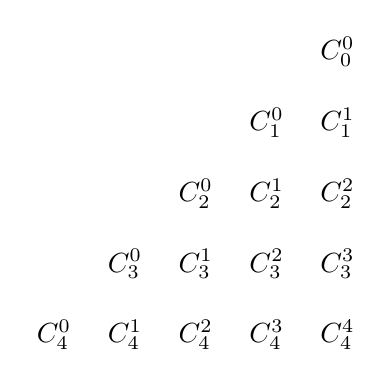
\begin{tikzpicture}[scale=0.9]
            \node[black] at (0,0) {$C_0^0$};
            \node[black] at (-1,-1) {$C_1^0$};
            \node[black] at (0,-1) {$C_1^1$};
            \node[black] at (-2,-2) {$C_2^0$};
            \node[black] at (-1,-2) {$C_2^1$};
            \node[black] at (-0,-2) {$C_2^2$};
            \node[black] at (-3,-3) {$C_3^0$};
            \node[black] at (-2,-3) {$C_3^1$};
            \node[black] at (-1,-3) {$C_3^2$};
            \node[black] at (-0,-3) {$C_3^3$};
            \node[black] at (-4,-4) {$C_4^0$};
            \node[black] at (-3,-4) {$C_4^1$};
            \node[black] at (-2,-4) {$C_4^2$};
            \node[black] at (-1,-4) {$C_4^3$};
            \node[black] at (-0,-4) {$C_4^4$};
        \end{tikzpicture}
        \hspace{2.5em}
        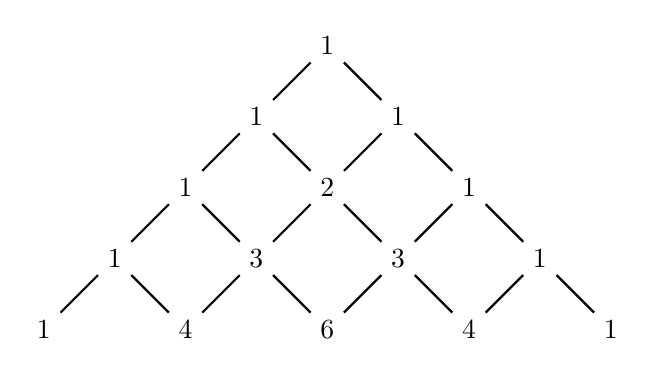
\begin{tikzpicture}[scale=0.9]
            \node[black] (0) at (0,0) {1};
            \node[black] (1) at (-1,-1) {1};
            \node[black] (2) at (1,-1) {1};
            \node[black] (3) at (-2,-2) {1};
            \node[black] (4) at (0,-2) {2};
            \node[black] (5) at (2,-2) {1};
            \node[black] (6) at (-3,-3) {1};
            \node[black] (7) at (-1,-3) {3};
            \node[black] (8) at (1,-3) {3};
            \node[black] (9) at (3,-3) {1};
            \node[black] (10) at (-4,-4) {1};
            \node[black] (11) at (-2,-4) {4};
            \node[black] (12) at (0,-4) {6};
            \node[black] (13) at (2,-4) {4};
            \node[black] (14) at (4,-4) {1};
            \draw[-,thick] (0) to (1);
            \draw[-,thick] (0) to (2);
            \draw[-,thick] (1) to (3);
            \draw[-,thick] (1) to (4);
            \draw[-,thick] (2) to (4);
            \draw[-,thick] (2) to (5);
            \draw[-,thick] (3) to (6);
            \draw[-,thick] (3) to (7);
            \draw[-,thick] (4) to (7);
            \draw[-,thick] (4) to (8);
            \draw[-,thick] (5) to (8);
            \draw[-,thick] (5) to (9);
            \draw[-,thick] (6) to (10);
            \draw[-,thick] (6) to (11);
            \draw[-,thick] (7) to (11);
            \draw[-,thick] (7) to (12);
            \draw[-,thick] (8) to (12);
            \draw[-,thick] (8) to (13);
            \draw[-,thick] (9) to (13);
            \draw[-,thick] (9) to (14);
        \end{tikzpicture}

        \subsection{阶乘与双阶乘}

        \begin{enumerate}
            \item $n!=1\times 2\times 3\times\cdots\times n$,其中$0!=1$。
            \item $(2n)!!=2\times 4\times 6\times\cdots\times(2n)=2^n\cdot n!$。
            \item $(2n-1)!!=1\times 3\times 5\times\cdots\times(2n-1)$。
        \end{enumerate}

        以后的华里士公式(点火公式,在定积分中)会使用到,如下面的题目:

        \textbf{例题:}计算$\int_0^{\frac{\pi}{2}}\sin^{10}x\textrm{d}x$与$\int_0^{\frac{\pi}{2}}\cos^9x\textrm{d}x$。\medskip

        解:原式1为偶数次幂,所以$=\dfrac{9}{10}\cdot\dfrac{7}{8}\cdot\dfrac{5}{6}\cdot\dfrac{3}{4}\cdot\dfrac{1}{2}\cdot\dfrac{\pi}{2}=\dfrac{\pi}{2}\cdot\dfrac{9!!}{10!!}$。\medskip

        原式2为奇数次幂,所以$=\dfrac{8}{9}\cdot\dfrac{6}{7}\cdot\dfrac{4}{5}\cdot\dfrac{2}{3}=\dfrac{8!!}{9!!}$

        \subsection{常用不等式}

        非常重要。

        \subsubsection{绝对值不等式}

        若$a$,$b$为实数,则:

        \begin{enumerate}
            \item $\vert a\pm b\vert\leqslant\vert a\vert+\vert b\vert$。
            \item 推广公式一到离散区间:$\vert a_1\pm a_2\pm a_3\pm\cdots\pm a_n\vert\leqslant\vert a_1\vert+\vert a_2\vert+\cdots+\vert a_n\vert$。
            \item 推广公式一到连续区间且$f(x)$在$[a,b](a<b)$上可积:$\vert\int_a^bf(x)\textrm{d}x\vert\leqslant\int_a^b\vert f(x)\vert\textrm{d}x$。因为符号不一定相同的面积代数和一定小于同为正的面积代数和。
            \item $\vert\vert a\vert-\vert b\vert\vert\leqslant\vert a-b\vert$。后式子为两点之差,前式子可以看作$a$、$b$两点与0之间的距离的差,若异号则两者必然抵消一部分,若同号则就等于后式。
        \end{enumerate}



        \subsubsection{根号不等式}

        公式一非常重要,即算数平均值大几何平均值。

        $a,b,c>0$:

        \begin{enumerate}
            \item $\sqrt{ab}\leqslant\dfrac{a+b}{2}\leqslant\sqrt{\dfrac{a^2+b^2}{2}}$。
            \item $\sqrt[3]{abc}\leqslant\dfrac{a+b+c}{3}\leqslant\dfrac{a^2+b^2+c^2}{3}$。
        \end{enumerate}

        \textbf{例题:}证明函数$f(x)=\dfrac{x}{1+x^2}$在$(-\infty,+\infty)$内有界。

        证明:可以使用极限,若极限存在则函数有界,这里使用有界性定义与不等式来完成。

        \ding{172}当$x=0$时,$f(0)=\dfrac{0}{1}$,有界。

        \ding{173}当$x\neq 0$时,原式分式上下都有$x$,所以简化公式:$f(x)=\dfrac{\dfrac{x}{x}}{\dfrac{1+x^2}{x}}=\dfrac{1}{\dfrac{1}{x}+x}$。

        $\because$需要证明有界性,以及根号不等式下需要参数大于0,所以需要证明$\vert f(x)\vert=\dfrac{1}{\dfrac{1}{\vert x\vert}+\vert x\vert}\leqslant M$

        又$\because\dfrac{a+b}{2}\geqslant\sqrt{ab}$,$\therefore \dfrac{\dfrac{1}{\vert x\vert}+\vert x\vert}{2}\geqslant\sqrt{\dfrac{1}{\vert x\vert}\cdot\vert x\vert}=1$

        $\therefore\vert f(x)\vert=\dfrac{1}{\dfrac{1}{\vert x\vert}+\vert x\vert}\leqslant\dfrac{1}{2}$。

        故整个函数在$R$上有界。

        \subsubsection{指数不等式}

        设$a>b>0$,则$
        \left\{
        \begin{array}{lcl}
            a^n>b^n,   &  & \text{当}n>0\text{时} \\
            a^n<b^n, &  & \text{当}n<0\text{时}
        \end{array}
        \right.$。

        $e^x\geqslant x+1(\forall x)$。

        \subsubsection{分数不等式}

        若$0<a<x<b,0<c<y<d$,则$\dfrac{c}{b}<\dfrac{y}{x}<\dfrac{d}{a}$。

        \subsubsection{三角不等式}

        \begin{enumerate}
            \item $\sin x<x<\tan x(0<x<\dfrac{\pi}{2})$。
            \item $\sin x<x(x>0)$。
            \item $\arctan x\leqslant x\leqslant\arcsin x(0\leqslant x\leqslant 1)$。
        \end{enumerate}

        \subsubsection{对数不等式}

        \begin{enumerate}
            \item $x-1\geqslant\ln x(x>0)$。
            \item $\dfrac{1}{1+x}<\ln(1+\dfrac{1}{x})<\dfrac{1}{x}(x>0)$。
        \end{enumerate}

        \section{映射与函数}
        \subsection{邻域}
        \subsubsection{一维}

        邻域\textcolor{violet}{\textbf{定义:}}以点$x_0$为中心的任何开区间为点$x_0$的邻域,记为$U(x_0)$。

        $\delta$邻域\textcolor{violet}{\textbf{定义:}}设$\delta$为一正数,则称开区间$(x_0-\delta,x_0+\delta)$为点$x_0$的$\delta$邻域,记作$U(x_0,\delta)$。$x_0$称为邻域的中心,$\delta$为邻域的半径。

        去心$\delta$邻域就是去除$x_0$的$\delta$邻域,记为$\mathring{U}(x_0,\delta)$,左$\delta$邻域就是左侧的去心$\delta$邻域,记为$U^+(x_0,\delta)$,右$\delta$邻域就是右侧的去心$\delta$邻域,记为$U^-(x_0,\delta)$。

        \subsubsection{二维}

        邻域\textcolor{violet}{\textbf{定义:}}设点$P_0(x_0,y_0)$为$xOy$平面上的一点,$\delta$为某一个正数,与点$P_0(x_0,y_0)$的距离小于$\delta$的点$P(x,y)$的全体,称为点$P_0$的$\delta$邻域,记为$U(P_0,\delta)$。

        同理可以得到去心$\delta$邻域的定义。

        $\delta$邻域的几何意义:以$P_0(x_0,y_0)$为中心,以$\delta>0$为半径的圆内部所有的点。

        函数的邻域就是一个区间,所以比如函数在某点的某邻域内有定义,就是说明函数在这个点的附近有定义,这个附近的距离没有必要说明。

        \subsection{函数的概念}
        \subsubsection{函数}

        \begin{itemize}
            \item 函数即$y=f(x),x\in D$,$x$为自变量,$y$为因变量,$D$为定义域。
            \item 一个$x$对应一个$y$,一个$y$可能对应多个$x$。
        \end{itemize}
        \subsubsection{反函数}

        $y=f(x)$,定义域为$D$,值域为$R$,若对于每一个$y\in R$,必然存在$x\in D$使$y=f(x)$成立,则可以定义一个新函数$x=\psi(y)$,这个函数就是$y=f(x)$的\textbf{反函数},一般记作$x=f^{-1}(y)$,其定义域为$R$,值域为$D$,对于反函数,原来的函数称为\textbf{直接函数}。
        \begin{enumerate}
            \item \textcolor{red}{严格单调}函数必然有反函数,即函数导数恒正或恒负必然有反函数。
            \item $x=f^{-1}(y)$与$y=f(x)$在同一坐标系中完全重合。
            \item $y=f^{-1}(x)$与$y=f(x)$关于$y=x$对称。
            \item $f[f^{-1}(x)]$($f[\psi(x)]$)或$f^{-1}[f(x)]=x$($\psi[f(x)]$)变为$x$,称为湮灭。
        \end{enumerate}

        可以验算一下性质四。

        已知$y=e^x$和$y=\ln x$是一对反函数,$y=\ln e^x=f^{-1}(f(x))=x$。

        反函数的求法:

        \begin{enumerate}
            \item 求值域。
            \item 求解。(用$y$表示$x$)
            \item 互换$xy$。
        \end{enumerate}

        \textbf{例题:}若函数$y=f(x)$的反函数为$y=f^{-1}(x)$,则求$y=f(2x-1)+1$的反函数的解析式。

        解:整理$y=f(2x-1)+1$,得到$f(2x-1)=y-1$,所以求反函数就是交换$xy$。

        这里将$2x-1$当作$x$,$y-1$当作$y$,所以得到反函数$2x-1=f^{-1}(y-1)$。

        所以得到$x=\dfrac{f^{-1}(y-1)+1}{2}$。

        所以交换表示方法其反函数就是$y=\dfrac{f^{-1}(x-1)+1}{2}$。

        \textbf{例题:}已知$f(x)=\dfrac{1}{1-x^2}$($x<-1$),求$f^{-1}(-\dfrac{1}{3})$。

        解:由于是反函数,所以$x$对应$y$,$y$对应$x$。

        求$f^{-1}(-\dfrac{1}{3})$的值,对应反函数的$x=-\dfrac{1}{3}$,$y=f^{-1}(-\dfrac{1}{3})$的值。

        即求原函数的$y=-\dfrac{1}{3}$,$x=f(-\dfrac{1}{3})$的值。

        所以$\dfrac{1}{1-x^2}=-\dfrac{1}{3}$求$x$的值。

        即$1-x^2=-3$,$x=\pm2$,又$x<-1$,则$x=-2$。

        \textbf{例题:}已知$f(x)=\dfrac{1-2x}{1+x}$,函数$g(x)$的图像与函数$y=f^{-1}(x+1)$的图像关于$y=x$对称,求$g(5)$。

        解:由于函数$g(x)$的图像与函数$y=f^{-1}(x+1)$的图像关于$y=x$对称,所以$g(x)$与$f^{-1}(x+1)$也是反函数。

        所以要求$g(x)$,就要求$f^{-1}(x+1)$。

        $\because y=f^{-1}(x+1)$,$\therefore x+1=f(y)$,$x=f(y)-1$,即$y=f(x)-1$。

        $\therefore g(x)=y=f(x)-1$,$g(5)=f(5)-1=-\dfrac{5}{2}$。

        \textbf{例题:}已知$f(x)=\dfrac{1}{2}(x^2+\sqrt{x+1})$($x\geqslant0$)的反函数为$f^{-1}(x)$,求不等式$f^{-1}(x+1)>3$的解集。

        解:当$x\geqslant0$时,$f(x)$明显是一个单调递增函数,所以根据反函数性质,其反函数在这个区间上增减性不变也是递增的。

        $f(0)=\dfrac{1}{2}$,即$f^{-1}(x)$在定义域$[\dfrac{1}{2},+\infty)$上也是递增函数。

        又$f^{-1}(x+1)>3$,对其求反函数:$f(f^{-1}(x+1))>f(3)$,即$x+1>f(3)$,且$x+1\geqslant\dfrac{1}{2}$,得出$x>\dfrac{9}{2}$。

        \textbf{例题:}求函数$y=f(x)=\ln(x+\sqrt{x^2+1})$的反函数$f^{-1}(x)$的表达式及其定义域。

        解:首先研究$f(x)$本身,因为$\ln(x)$的定义域必然要求大于0,而任意实数$x$都有下面不等式成立:

        $x+\sqrt{x^2+1}>x+\vert x\vert \geqslant 0$,所以$x\in R$。

        而研究其奇偶性:

        $f(-x)=\ln(-x+\sqrt{x^2+1})=\ln(\dfrac{1}{\sqrt{x^2+1}+x})=-\ln(x+\sqrt{x^2+1})=-f(x)$

        所以该函数为奇函数。

        对其求单调性,即通过链式法则求导:

        $\dfrac{\rm{d}\textit{y}}{\rm{d}\textit{x}}=\dfrac{1}{x+\sqrt{x^2+1}}\cdot (1+\dfrac{2x}{2\sqrt{x^2+1}})=\dfrac{1}{\sqrt{x^2+1}}>0$。\medskip

        所以该函数严格单调增。

        然后求$y$的反函数:

        $\because y=\ln(x+\sqrt{x^2+1})$,对于对数函数就要把它变为指数函数:

        $e^y=e^{\ln(x+\sqrt{x^2+1})}=x+\sqrt{x^2+1}$

        $
        \begin{aligned}
            \because -y & =-\ln(x+\sqrt{x^2+1})          \\
            & =\ln(\dfrac{1}{x+\sqrt{x^2+1}}) \\
            & =\ln(\sqrt{x^2+1}-x)           \\
            e^{-y}      & =\sqrt{x^2+1}-x
        \end{aligned}
        $

        $
        \begin{aligned}
            \therefore e^y-e^{-y} & =2x                   \\
            x                     & =\dfrac{e^y-e^{-y}}{2}
        \end{aligned}
        $

        解出了用$x$表示$y$的函数表达$x=f^{-1}(y)$,即反函数,则$f^{-1}(x)=\dfrac{e^x-e^{-x}}{2}$

        这种曲线为一种常见曲线:

        \begin{itemize}
            \item $\dfrac{e^x-e^{-x}}{2}$:双曲正弦。
            \item $\dfrac{e^x+e^{-x}}{2}$:双曲余弦。(为一种悬链线)
            \item $\ln(x+\sqrt{x^2+1})$:反双曲正弦。
            \item $\ln(x+\sqrt{x^2-1})$:反双曲余弦。
        \end{itemize}

        \subsubsection{复合函数}
        设$y=f(u)$的定义域为$D_1$,函数$u=g(x)$在$D$上有定义且$g(D)\in D$,则由$y=f[g(x)],x\in D$确定的函数称为由函数$u=g(x)$和函数$y=f(u)$构成的复合函数,定义域为$D$,$u$为中间变量。

        \textbf{例题:}设$f(x)=x^2$,$f[\psi(x)]=-x^2+2x+3$,且$\psi(x)\geqslant 0$,求$\psi(x)$以及定义域与值域。

        解:广义化:$\because f(x)=x^2$,$\therefore f[\psi(x)]=\psi^2(x)=-x^2+2x+3$

        又$\because\psi(x)\geqslant 0$, $\therefore\sqrt{\psi^2(x)}=\sqrt{-x^2+2x+3}=\psi(x)\geqslant 0$

        $\therefore x\in[-1,3]$

        $\therefore\dfrac{\rm{d}\psi(\textit{x})}{\rm{d}\textit{x}}=(-x^2+2x+3)'=-2x+2=0$

        $\therefore x=1$,驻点为1

        又$\because(-x^2+2x+3)''=-2<0$

        $\therefore$驻点为1时为最大值点,最大值为$\psi(1)=2$

        又$\because\psi(-1)=\psi(3)=0$,$\therefore$最小值为0

        $\therefore\psi(x)\in[0,2]$

        \textcolor{orange}{注意}:$\sqrt{-x^2+2x+3}$为什么最值与$-x^2+2x+3$一致?

        \textbf{例题:}设$
        f(x)=\left\{
        \begin{array}{lcl}
            \ln\sqrt{x}, &  & x\geqslant 1 \\
            2x-1,        &  & x< 1
        \end{array}
        \right.
        $,求$f[f(x)]$

        首先广义化:$
        f[f(x)]=\left\{
        \begin{array}{lcl}
            \ln\sqrt{f(x)}, &  & f(x)\geqslant 1 \\
            2f(x)-1,        &  & x<1
        \end{array}
        \right.
        $

        分段点为$1$,然后对$f(x)$画图:\medskip

        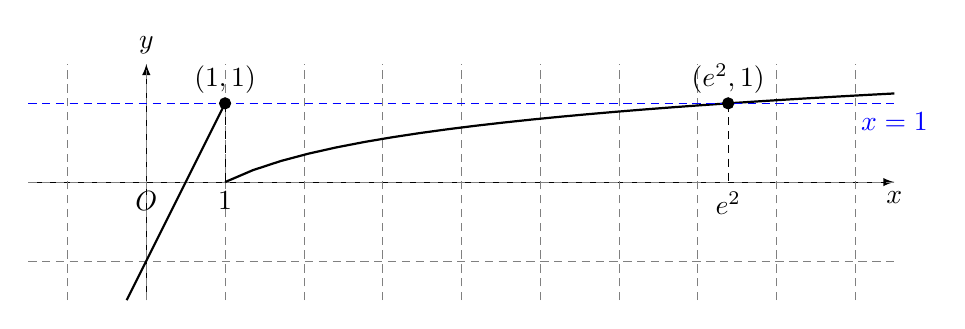
\begin{tikzpicture}[domain=-1:9.5]
            \draw[-latex](-1.5,0) -- (9.5,0) node[below]{$x$};
            \draw[-latex](0,-1.5) -- (0, 1.5) node[above]{$y$};
            \draw[very thin, gray, densely dashed](-1.5,1.5)grid(9.5,-1.5);
            \draw[black, thick](-0.25,-1.5) -- (1,1);
            \draw[black, thick,domain=1:9.5] plot (\x, {ln(sqrt(\x))});
            \draw[blue, densely dashed](-1.5,1) -- (9.5,1) node[below]{$x=1$};
            \filldraw[black] (1,1) circle (2pt) node[above]{$(1,1)$};
            \filldraw[black] (e^2,1) circle (2pt) node[above]{$(e^2,1)$};
            \draw[densely dashed](1,1) -- (1, 0) node[below]{$1$};
            \draw[densely dashed](e^2,1) -- (e^2,0) node[below]{$e^2$};
            \filldraw[black] (0,0) node[below]{$O$};
        \end{tikzpicture}

        所以将定义域分为三段:$[-\infty ,1],[1,e^2],[e^2, +\infty]$,然后根据不同定义域对应的不同函数再代回$f[f(x)]$:

        $$
        f[f(x)]=\left\{
        \begin{array}{lcl}
            \ln\sqrt{\ln\sqrt{x}}, &  & x\geqslant e^2   \\
            \ln x-2,               &  & 1\geqslant x<e^2 \\
            4x-3,                  &  & x<1
        \end{array}
        \right.
        $$

        \subsection{函数的特性}

        \subsubsection{有界性}

        \textcolor{violet}{\textbf{定义:}}函数$f(x)$的定义域$D$,数集$I\in D$,如果存在某正数$M$,对于任一$x\in I$,有$\vert f(x)\vert\leqslant M$,则$f(x)$在$I$上有界,否则无界。

        函数指明定义域区间才能讨论函数是否有界。

        如果$f(x)\geqslant M$有下界,$f(x)\leqslant M$则有上界。

        \subsubsection{单调性}

        \textcolor{violet}{\textbf{定义:}}$y=f(x)$,$x\in D$,如果$\forall x_1,x_2\in D$且$x_1<x_2$,有$f(x_1)<f(x_2)$,则函数在$D$上单调递增。反之则单调递减。

        \medskip

        $\begin{matrix}
             \dfrac{\rm{d}\textit{y}}{\rm{d}\textit{x}}>0 & \Rightarrow & (x_1-x_2)[f(x_1)-f(x_2)]>0 & \Rightarrow & f(x)\nearrow \\
             \dfrac{\rm{d}\textit{y}}{\rm{d}\textit{x}}<0 & \Rightarrow & (x_1-x_2)[f(x_1)-f(x_2)]<0 & \Rightarrow & f(x)\searrow
        \end{matrix}
        $

        \subsubsection{奇偶性}

        \begin{enumerate}
            \item 奇函数:关于原点对称,$f(-x)=-f(x)$。
            \item 偶函数:关于$y$轴对称,$f(-x)=f(x)$。
            \item 对于定义在$[-l,l]$上的任意函数$f(x)$,$F_1(x)=f(x)-f(-x)$必为奇函数,$F_2(x)=f(x)+f(-x)$必为偶函数。可以参考上面所说的双曲正弦与双曲余弦函数。
            \item 若奇函数在0处有定义,那么$f(0)=0$。
            \item 若偶函数在0处存在导数,那么$f'(0)=0$,即$x=0$,曲线必然水平,即导数为0。
            \item 若函数$y=f(x)$的函数关于直线$x=T$对称的充分必要条件是$f(x)=f(2T-x)/f(x+T)=f(x-T)$。(令$T-x=t$进行换元计算得到)
        \end{enumerate}

        无论$f(x)$是什么函数,$F(x)=f(x)+f(-x)$都是偶函数,$G(x)=x(f(x)+f(-x))$都是奇函数。

        \subsubsection{周期性}

        $f(x+T)=f(x)$,其中$T$为周期。 \medskip

        \subsubsection{重要结论}

        \begin{enumerate}
            \item 若$f(x)$为可导的偶函数,则$f'(x)$为奇函数。
            \item 若$f(x)$为可导的奇函数,则$f'(x)$为偶函数。
            \item 若$f(x)$为周期函数,则$f'(x)$也为周期函数且周期不变。
            \item 连续的奇函数的一切原函数都是偶函数。
            \item 连续的偶函数的原函数中仅有一个原函数是奇函数。
            \item 若连续函数$f(x)$以$T$为周期且$\int_{0}^{T}f(x)\rm{d}\textit{x}=0$,则$f(x)$的一切原函数也以$T$为周期。
            \item 若$f(x)$在有限区间$(a,b)$中可导且$f'(x)$有界,则$f(x)$在$(a,b)$有界。(某一函数在固定区间内变化率是有界的,则变化范围是有界的)
        \end{enumerate}

        \textcolor{orange}{注意}:0和1处的函数定义应该注意。

        如当a为0时:$f(b)-f(a)=f'(\xi )(b-a)=f(b)=bf'(\xi)$

        如$f(x)>xf(1)$变形为$\dfrac{f(x)}{x}>f(1)$,辅助函数$F(x)=\dfrac{f(x)}{x}$

        所以加减法警惕0,乘除法警惕1。

        \section{数列的极限}

        极限就是一个无限逼近某个值的过程。如$\dfrac{n}{n+1}$这个分式在$n$无限增大的时候会无限逼近1,这个1叫做极限值,所以写成$\lim\limits_{n\to\infty}\dfrac{n}{n+1}=1$。

        所以从另一个方面更精确的指出一个数$N>0$,使得数列下标大于$N$的项与极限值之间的距离始终保持在$(0,\xi)$之间,即$\dfrac{1}{n+1}<\xi$,即$n>\dfrac{1}{\xi}-1$,所以任意正数都能得到从$N>\dfrac{1}{\xi}-1$项开始之后都有$\left\vert\dfrac{n}{n+1}-1\right\vert<\xi$。

        \subsection{定义}

        通过定义可以证明极限。

        \subsubsection{数列极限定义}

        \textcolor{violet}{\textbf{定义:}}设$\{x_n\}$为一数列,若存在常数$a$,对于不论任意小的$\xi>0$,总存在正整数$N$,使$n>N$时,$\vert x_n-a\vert<\xi$恒成立,则常数$a$为数列$\{x_n\}$的极限,或$\{x_n\}$收敛于$a$,记为:$\lim\limits_{x\to\infty}x_n=a$或$x_n\to a(n\to\infty)$。

        常用语言($\xi-N$语言):$\lim\limits_{x\to\infty}x_n=a\Leftrightarrow\forall\xi>0,\exists N\in N_+$,当$n>N$时,恒有$\vert x_n-a\vert<\xi$。

        如果不存在该数$a$,则称数列$x_n$发散。

        即无论给出多么小的$\xi$,总可以找到一项从该项之后函数值与极限值之间的差小于$\xi$,即更接近这个极限值而不是其他任何值,所以该数列趋向于极限值。

        \subsubsection{极限证明}

        令$x_n$为通项,$a$为极限值,$\xi$为任意正数。

        \begin{enumerate}
            \item 写出$\vert x_n-a|<\xi$。
            \item 反解出项数$n<g(\xi)$。
            \item 取$N=[g(\xi)]+1$,所以令$n>N$就可以证明。
        \end{enumerate}

        \textbf{例题:}用定义证明$\lim\limits_{x\to\infty}\left[1+\dfrac{(-1)^n}{n}\right]=1$

        证明:\ding{172}计算距离:$\left\vert 1+\dfrac{(-1)^n}{n}-1\right\vert=\left\vert\dfrac{(-1)^n}{n}\right\vert<\xi$。

        \ding{173}解得到:$\dfrac{1}{n}<\xi$,反解为$n>\dfrac{1}{\xi}$。

        \ding{174}取整:$N=\left[\dfrac{1}{\xi}\right]+1$。

        $\therefore\forall\xi>0$,当$n>N$时,就有$n>\dfrac{1}{\xi}$,使得$\left\vert 1+\dfrac{(-1)^n}{n}-1\right\vert=\left\vert\dfrac{(-1)^n}{n}\right\vert<\xi$。

        $\therefore$证明完毕。

        \textbf{例题:}用定义证明$\lim\limits_{n\to\infty}q^n=0$($q$为常数且$\vert q\vert<1$)。

        证明:\ding{172}$\vert q^n-0\vert<\xi$。

        \ding{173}$\vert q^n\vert<\xi$,取对数进行反解$n\ln\vert q\vert<\ln\xi$,又因为$\vert q\vert<1$,所以$\ln\vert q\vert<0$,所以得到$n>\dfrac{\ln\xi}{\ln\vert q\vert}$。(若$\xi>1$则$n$就是负数,这样条件必然成立)

        \ding{174}取$N=\left[\dfrac{\ln\xi}{\ln\vert q\vert}\right]+1$。

        $\therefore$当$n>N$时,必然$n>\dfrac{\ln\xi}{\ln\vert q\vert}$,有$\vert q^n-0\vert<\xi$。

        故$\lim\limits_{n\to\infty}q^n=0$。

        \subsubsection{数列绝对值}

        \textcolor{aqua}{\textbf{定理:}}若$\lim\limits_{x\to\infty}a_n=A$,则$\lim\limits_{x\to\infty}\vert a_n\vert=\vert A\vert$。

        证明:$\because\lim\limits_{n\to\infty}a_n=A\Leftrightarrow\forall\xi>0,\exists N>0,\text{当}n>N$,恒有$\vert a_n-A\vert<\xi$。

        又由重要不等式$\vert\vert a\vert-\vert b\vert\vert\leqslant\vert a-b\vert$,所以$\vert\vert a_n\vert-\vert A\vert\vert\leqslant\xi$。

        所以恒成立,证明完毕。

        从这个题推出:$\lim\limits_{n\to\infty}a_n=0\Leftrightarrow\lim\limits_{n\to\infty}\vert a_n\vert=0$。所以如果我们以后需要证明某一数列极限为0,可以证明数列绝对值极限0,而数列绝对值绝对时大于等于0的,所以由夹逼准则,其中小的一头已经固定为0了,所以只用找另一个偏大的数列夹逼所证明数列就可以了。

        \subsubsection{子数列}

        \textcolor{violet}{\textbf{定义:}}从数列${a_n}:a_1,a_2,\cdots,a_n,\cdots$中选取无穷多项并按原来顺序组成的新数列就称为原数列的子列,记为$\{a_{n_k}\}:a_{n_1},a_{n_2},\cdots,a_{n_k},\cdots$。

        若$n_k$分别取奇数和偶数,则得到奇数项数列与偶数项数列。

        \textcolor{aqua}{\textbf{定理:}}若数列$\{a_n\}$收敛,则其任何子列$\{a_{n_k}\}$也收敛,且极限值相同。

        所以对于其变式我们用到更多:

        \begin{enumerate}
            \item 若一个数列$\{a_n\}$能找到一个发散的子列,那该数列发散。
            \item 若一个数列$\{a_n\}$能找到两个极限值不同的收敛子列,那么这个数列发散。
            \item 若一个数列$\{a_n\}$,则其奇数子列与偶数子列都收敛于同一个值。
        \end{enumerate}

        例如对于数列$\{(-1)^n\}$,能找到其奇数子列收敛于-1,偶数子列收敛于1,所以收敛值不同,原数列发散。

        \subsection{性质}
        \subsubsection{唯一性}

        \textcolor{violet}{\textbf{定义:}}若数列$\{x_n\}$收敛于$a$,则$a$是唯一的。

        证明:设$\lim\limits_{n\to\infty}a_n=A$且$\lim\limits_{n\to\infty}a_n=B$且$A\neq B$。

        不如设$A>B$。任意取$\xi=\dfrac{A-B}{2}>0$。

        $\because\lim\limits_{n\to\infty}a_n=A$

        $\therefore\exists N_1>0$,当$n>N_1$时,$\vert a_n-A\vert<\dfrac{A-B}{2}$。

        得到$\dfrac{A+B}{2}<a_n<\dfrac{3A-B}{2}$并设为式子一。

        又$\because\lim\limits_{n\to\infty}a_n=B$

        $\therefore\exists N_2>0$,当$n>N_2$时,$\vert a_n-B\vert<\dfrac{A-B}{2}$。

        得到$\dfrac{3A-B}{2}<a_n<\dfrac{A+B}{2}$并设为式子二。

        取$N=\max\{N_1,N_2\}$,当$n>N$时,式子一二同时成立,而$A\neq B$,则这两个式子不可能同时成立,矛盾。

        同理$A<B$时也矛盾,所以$A\neq B$矛盾。

        \subsubsection{有界性}

        \textcolor{violet}{\textbf{定义:}}若数列$\{x_n\}$极限存在,则数列有界。

        即$\lim\limits_{n\to\infty}a_n=A$,则存在$M>0$,使得$\vert a_n\vert\leqslant M$。

        证明:由极限定义,取$\xi=1$。

        $\because\lim\limits_{n\to\infty}a_n=A$

        $\therefore\exists N>0$,当$n>N$时,$\vert a_n-A\vert<1$。

        $\because\text{重要不等式}\,\vert\vert a_n\vert-\vert A\vert\vert\leqslant\vert a_n-A\vert$

        $\therefore n>N$时,$\vert\vert a_n\vert-\vert A\vert\vert<1\Rightarrow\vert a_n\vert<1+\vert A\vert$

        取$M=\max\{\vert a_1\vert,\vert a_2\vert,\cdots,\vert a_N\vert,1+\vert A\vert\}$

        $\forall n$,有$\vert a_n\vert\leqslant M$

        所以数列极限存在则数列有界。

        但是数列有界不一定极限存在,如$1+(-1)^n$。

        \subsubsection{保号性}

        较重要。也称为脱帽法。

        \textcolor{violet}{\textbf{定义:}}若数列$\{x_n\}$存在极限$\lim\limits_{n\to\infty}a_n=a\neq 0$,则存在正整数$N$,当$n>N$时$a_n$都与$a$同号。

        简单来说,就是极限大于0,后面一部分数列大于0,极限小于0,后面一部分数列小于0。

        推论,戴帽法:若数列$\{a_n\}$从某项开始$a_n\geqslant b$,且$\lim\limits_{n\to\infty}a_n=a$,则$a\geqslant b$。这里一定要带等号。

        证明:设$A>0$,取$\xi=\dfrac{A}{2}>0$。

        $\because\lim\limits_{n\to\infty}a_n=A$

        $\therefore\exists N>0$,当$n>N$时,$\vert a_n-A\vert<\dfrac{A}{2}\Rightarrow a_n>\dfrac{A}{2}>0$

        同理得证极限值小于0的情况。

        \subsection{海涅定理(归结原则)}

        \textcolor{aqua}{\textbf{定理:}}设$f(x)$在$\mathring{U}(x_0,\delta)$内有定义,则$\lim\limits_{x\to x_0}f(x)=A$存在$\Leftrightarrow$对任何$\mathring{U}(x_0,\delta)$内以$x_0$为极限的数列$\{x_n\}(x_n\neq x_0)$,极限$\lim\limits_{n\to\infty}f(x_n)=A$存在。

        海涅定理用来连接数列极限与函数极限。在极限存在下他们可以相互转换。

        \textbf{例题:}求$\lim\limits_{n\to\infty}\left(n\tan\dfrac{1}{n}\right)^{n^2}$($n\in N^+$)。

        解:首先将式子由数列极限变为函数极限,并取$x=\dfrac{1}{n}$:$\lim\limits_{x\to 0}\left(\dfrac{\tan x}{x}\right)^{\frac{1}{x^2}}$。

        又$u^v=e^{v\ln u}$,对式子取指数$\therefore =e^{\lim\limits_{x\to 0}\frac{1}{x^2}\ln\frac{\tan x}{x}}$

        又在$x\to 0$下使用等价无穷小$\ln (1+x)\sim x$,$\therefore \ln(1+g(x))\sim g(x),g(x)\to 0$。

        而在$x\to 0$时,根据等价无穷小$\tan x\sim x$,所以$\dfrac{\tan x}{x}$趋于1,不满足趋于0的条件。

        所以正好将$\ln\dfrac{\tan x}{x}$变形$\ln\left(1+\dfrac{\tan x}{x}-1\right)$。

        $\therefore \ln\left(1+\dfrac{\tan x}{x}-1\right)\sim\dfrac{\tan x}{x}-1$,$\dfrac{\tan x}{x}-1\to 0$。

        又根据泰勒展开$\tan x-x=x+\dfrac{x^3}{3}+o(x^3)-x-0\cdot x^3=\dfrac{x^3}{3}$。

        $\therefore e^{\lim\limits_{x\to 0}\frac{1}{x^2}\ln\frac{\tan x}{x}}=e^{\lim\limits_{x\to 0}\frac{1}{x^2}\frac{\tan x-x}{x}}=e^{\lim\limits_{x\to 0}\frac{1}{x^2}\cdot\frac{x^2}{3}}=e^{\frac{1}{3}}$

        根据海涅定理:取$x=\dfrac{1}{n},n\to\infty$,$\lim\limits_{n\to\infty}\left(n\tan\dfrac{1}{n}\right)^{n^2}=e^{\frac{1}{3}}$。

        \section{函数的极限}

        \subsection{函数极限定义}

        \subsubsection{极限定义}

        \textcolor{violet}{\textbf{定义:}}设函数$f(x)$在点$x_0$的某一个去心邻域有定义,若存在常数$A$,对于任意给定的$\xi>0$,总存在正数$\delta$,使得当$0<\vert x-x_0\vert<\delta$式,对应的函数值$f(x)$都满足不等式$\vert f(x)-A\vert <\xi$,则$A$就是函数$f(x)$当$x\to x_0$时的极限,记作$\lim\limits_{x\to x_0}f(x)=A$或$f(x)\rightarrow A(x\rightarrow x_0)$。

        写成$\xi-\delta$语言:$\lim\limits_{x\to x_0}f(x)=A\Leftrightarrow\forall\xi>0,\exists\delta>0,\text{当}0<\vert x-x_0\vert<\delta$时,有$\vert f(x)-A\vert<\xi$。

        而对于趋向无穷时,写成$\xi-X$语言:$\lim\limits_{x\to\infty}f(x)=A\Leftrightarrow\forall\xi>0,\exists X>0,\text{当}\vert x\vert>X$时,有$\vert f(x)-A\vert<\xi$。

        \textcolor{orange}{注意:}这里的趋向分为六种:$x\to x_0$、$x\to x_0^+$、$x\to x_0^-$、$x\to\infty$、$x\to\infty^+$、$x\to\infty^-$。

        \subsubsection{单侧极限}

        当$x\to x_0^-$存在的极限称为左极限,当$x\to x_0^+$存在的极限称为右极限。

        \subsubsection{函数极限存在条件}

        函数存在的充要条件是:

        \begin{enumerate}
            \item $\lim\limits_{x\to x_0}f(x)\Leftrightarrow\lim\limits_{x\to x_0^-}f(x)=\lim\limits_{x\to x_0^+}f(x)=A$。
            \item 函数脱帽法:$\lim\limits_{x\to x_0}f(x)\Leftrightarrow f(x)=A+\alpha(x),\lim\limits_{x\to x_0}\alpha(x)=0$,后面的$\alpha(x)$就是函数与极限值的误差。
        \end{enumerate}

        \subsubsection{极限情况总结}

        \begin{center}
            \begin{tabular}{|c|c|c|c|c|}
                \hline
                过程 & $n\to\infty$ & $x\to\infty$ & $x\to+\infty$ & $x\to-\infty$ \\ \hline
                时刻 & \multicolumn{4}{c|}{$N$} \\ \hline
                从此时刻以后 & $n>N$ & $\vert x\vert>N$ & $x>N$ & $x<-N$ \\ \hline
                $f(x)$ & \multicolumn{4}{c|}{$\vert f(x)-A\vert<\xi$} \\
                \hline
            \end{tabular}
        \end{center}

        \begin{center}
            \begin{tabular}{|c|c|c|c|}
                \hline
                过程 & $x\to x_0$ & $x\to x_0^+$ & $x\to x_0^-$ \\ \hline
                时刻 & \multicolumn{3}{c|}{$\delta$} \\ \hline
                从此时刻以后 & $0<\vert x-x_0\vert<\delta$ & $0<x-x_0<\delta$ & $-\delta<x-x_0<0$\\ \hline
                $f(x)$ & \multicolumn{3}{c|}{$\vert f(x)-A\vert<\xi$} \\
                \hline
            \end{tabular}
        \end{center}

        \subsection{性质}

        与数列极限性质类似,且任何$x$的趋向三个性质都是成立的。

        \subsubsection{唯一性}

        \textcolor{violet}{\textbf{定义:}}若极限存在,则极限唯一。

        \subsubsection{局部有界性}

        \textcolor{violet}{\textbf{定义:}}若极限存在且为$A$,则存在正常数$M$和$\delta$,使得当$0<\vert x-x_0\vert<\delta$时,有$\vert f(x)\vert\leqslant M$。

        \begin{enumerate}
            \item 极限存在是函数局部有界性的充分不必要条件。
            \item $f(x)$在$[a,b]$上连续,则$f(x)$在$[a,b]$上有界。
            \item 有限个有界函数与有界函数的和、差、积仍是有界函数。
            \item 若$f'(x)$在有限区间$(a,b)$内有界,则$f(x)$在该区间内有界。
        \end{enumerate}

        对于结论二,可以利用极限存在必然连续的概念,对$f(x)$在区间两端求极限从而证明有界。这里两端的极限不要求是一样的,因为两端不一样的极限表明该趋向点的极限值不存在,但是仍然有界。

        证明结论四:

        利用中值定理:$f(b)-f(a)=f'(\xi)(b-a)$。

        令$x\in(a,b),x_0\in(a,b)$。其中这两个值不知道大小,只知道范围。

        代入中值定理:$f(x)-f(x_0)=f'(\xi)(x-x_0)$

        $
        \begin{aligned}
            \vert f(x)\vert & =\vert f(x_0)+f'(\xi)(x-x_0)\vert \\
            & \leqslant\vert f(x_0)\vert+\vert f'(\xi)\vert\vert x-x_0\vert\text{ (重要绝对值不等式)} \\
            & \leqslant\vert f(x_0)\vert+K\cdot(b-a) \\
            & \leqslant M
        \end{aligned}
        $

        \textbf{例题:}函数$f(x)=\dfrac{\vert x\vert\sin(x-2)}{x(x-1)(x-2)^2}$在哪个区间内有界()。\medskip

        $A.(-1,0)$\qquad$B.(0,1)$\qquad$C.(1,2)$\qquad$D.(2,3)$\medskip

        解:看选项,0,1,2出现次数较多,所以从$B$选项开始检查是否有界:\medskip

        $\lim\limits_{x\to 0^-}\dfrac{\vert x\vert\sin(x-2)}{x(x-1)(x-2)^2}=(-1)\cdot\dfrac{-\sin 2}{(-1)\cdot 4}=-\dfrac{\sin 2}{4}$\medskip

        所以趋于$0^-$的一段有界。\medskip

        同理$\lim\limits_{x\to 0^+}\dfrac{\vert x\vert\sin(x-2)}{x(x-1)(x-2)^2}=\dfrac{\sin 2}{4}$。\medskip

        所以趋于$0^+$的一段有界。\medskip

        $\lim\limits_{x\to 1^-}\dfrac{\vert x\vert\sin(x-2)}{x(x-1)(x-2)^2}$中$(x-1)$为0且在分母位置,所以极限为$\infty$,该区间无界。\medskip

        所以$(0,1)$无界,$B$排除。\medskip

        同理$\lim\limits_{x\to 1^+}\dfrac{\vert x\vert\sin(x-2)}{x(x-1)(x-2)^2}$也无穷大而无界。\medskip

        所以$(1,2)$无界,$C$排除。\medskip

        $\lim\limits_{x\to 2^+}\dfrac{\vert x\vert\sin(x-2)}{x(x-1)(x-2)^2}$中不管前面的项,而看到后面的$\dfrac{\sin(x-2)}{(x-2)^2}$。\medskip

        因为$\lim\limits_{x\to 0}\dfrac{\sin x}{x}=1$,所以对于$\lim\limits_{x\to 2}\dfrac{\sin(x-2)}{(x-2)}=1$,所以下面还有一个$x-2$,所以还是为$\infty$。

        所以$(2,3)$无界,$D$排除。\medskip

        验证-1处是否有界:\medskip

        $\lim\limits_{x\to -1}\dfrac{\vert x\vert\sin(x-2)}{x(x-1)(x-2)^2}=-\dfrac{\sin 3}{18}$。\medskip

        所以该处有界,所以选$A$。

        \subsubsection{局部保号性}

        \textcolor{violet}{\textbf{定义:}}若极限存在,则存在常数$\delta>0$,使得当$0<\vert x-x_0\vert<\delta$时,$f(x)$与$A$同号。

        简单来说,函数值在$x\to x_0$时函数值与极限值同号。

        证明:首先根据极限存在定义:$\forall\xi>0,\exists\delta>0,0<\vert x-x_0\vert<\delta$时,恒有$\vert f(x)-A\vert<\xi$。

        $\Rightarrow -\xi<f(x)-A<\xi$。

        $\Rightarrow A-\xi<f(x)<A+\xi$。

        任意取$\xi=\dfrac{A}{2}>0\Rightarrow f(x)>A-\dfrac{A}{2}=\dfrac{A}{2}>0$。

        证明完毕。

        关于$\xi$的取值问题,为什么不能取到令结果为负的值,因为请注意这个取值得到的区间并不是$f(x)$的范围,而是对$f(x)$所在区间的陈述,其是无尽逼近$A$的,所以取多大的区间都无所谓。

        推论:若函数值在$x\to x_0$时都非负或非正,极限值为$A$,那么$A$与此时函数值同号。不能去除等号。

        \medskip

        关于三个性质要注意自变量取值的双向性,所以需要留意下面几个函数:

        \begin{enumerate}
            \item $\lim\limits_{x\to\infty}e^x$不存在,因为$\lim\limits_{x\to +\infty}e^x=+\infty$,$\lim\limits_{x\to -\infty}e^x=0$。
            \item $\lim\limits_{x\to 0}\dfrac{\sin x}{\vert x\vert}$不存在,因为$\lim\limits_{x\to 0^+}\dfrac{\sin x}{\vert x\vert}=1$,$\lim\limits_{x\to 0^-}\dfrac{\sin x}{\vert x\vert}=-1$。
            \item $\lim\limits_{x\to\infty}\arctan x$不存在,因为$\lim\limits_{x\to +\infty}\arctan x=\dfrac{\pi}{2}$,$\lim\limits_{x\to -\infty}\arctan x=-\dfrac{\pi}{2}$。
            \item $\lim\limits_{x\to 0}[x]$不存在,因为$\lim\limits_{x\to 0^+}[x]=0$,$\lim\limits_{x\to 0^-}[x]=-1$
        \end{enumerate}

        \section{极限运算法则}

        \begin{enumerate}
            \item 有限个无穷小的和是无穷小。
            \item 有界函数与无穷小的乘积是无穷小。
            \item 有限个无穷小的乘积是无穷小。
        \end{enumerate}

        \subsection{数列极限}

        若$\lim\limits_{n\to\infty}x_n=a$,$\lim\limits_{n\to\infty}y_n=b$则:

        \begin{enumerate}
            \item $\lim\limits_{n\to\infty}x_n\pm y_n=a\pm b$。
            \item $\lim\limits_{n\to\infty}(x_ny_n)=\lim\limits_{n\to\infty}x_n\lim\limits_{n\to\infty}y_n=ab$。
            \item $\lim\limits_{n\to\infty}\dfrac{x_n}{y_n}=\dfrac{\lim\limits_{n\to\infty}x_n}{\lim\limits_{n\to\infty}y_n}=\dfrac{a}{b}(b\neq 0)$。
        \end{enumerate}

        \textbf{例题:}若$\lim\limits_{n\to\infty}(a_n+b_n)=1$且$\lim\limits_{n\to\infty}(a_n-b_n)=3$,计算$\lim\limits_{n\to\infty}a_n$与$\lim\limits_{n\to\infty}b_n$。

        解:首先是不能通过运算法则第一条将两个条件直接加减的,因为不能保证两个极限是否都存在。

        所以必须先令$u_n=a_n+b_n$,$v_n=a_n-b_n$,所以$\lim\limits_{n\to\infty}u_n=1$,$\lim\limits_{n\to\infty}v_n=3$。

        因为这两个极限都存在,所以可以进行运算。

        相加得到$\lim\limits_{n\to\infty}(u_n+v_n)=2\lim\limits_{n\to\infty}a_n=4$。

        所以得到$\lim\limits_{n\to\infty}a_n=2$。同理$\lim\limits_{n\to\infty}(u_n-v_n)$得到$\lim\limits_{n\to\infty}b_n=-1$。

        \subsection{函数极限}

        若$\lim f(x)=A$,$\lim g(x)=B$(即两个极限都存在),则

        \begin{enumerate}
            \item $\lim[k\cdot f(x)\pm l\cdot g(x)]=k\lim f(x)\pm l\cdot g(x)=kA\pm lB$,其中$kl$为常数。
            \item $\lim[f(x)\cdot g(x)]=\lim f(x)\cdot\lim g(x)=A\cdot B$
            \item $\lim[f(x)]^n=[\lim f(x)]^n$,其中$n$为正整数。
            \item $\lim\dfrac{f(x)}{g(x)}=\dfrac{\lim f(x)}{\lim g(x)}=\dfrac{A}{B}(B\neq 0)$。
            \item $\lim\limits_{x\to\infty}\dfrac{a_nx^n+a_{n-1}x^{n-1}+\cdots+a_1x+a_0}{b_mx^m+\cdots+b_{m-1}x^{m-1}+\cdots+b_1x+b_0}=\left\{
            \begin{array}{lcl}
                \dfrac{a_n}{b_m}, & & n=m \\
                0, & & n<m \\
                \infty, & & n>m
            \end{array}
            \right.$
            \item 若$f(x)\geqslant g(x)$,则$A\geqslant B$。
            \item 若$y=f[g(x)]$由$y=f(u)$与$u=g(x)$复合而成,且$\lim\limits_{x\to x_0}g(x)=u_0$且$\lim\limits_{u\to u_0}f(u)=a$,当$x\in\mathring{U}(x_0,\delta_0)$时,$g(x)\neq u_0$,则$\lim\limits_{x\to x_0}f[g(x)]=a$。
        \end{enumerate}

        对于结论7必须\textcolor{orange}{注意}$g(x)\neq u_0$。

        假设$f(u)=\dfrac{u^2-1}{u-1}$,所以这个$f(x)$在$x=1$处应无定义。但是这并不影响$\lim\limits_{u\to 1}f(u)=2$。

        假设$g(x)=\left\{
        \begin{array}{lcl}
            1+x, & & x<0 \\
            1, & & x>0
        \end{array}
        \right.$。

        则$\lim\limits_{x\to 0}g(x)=1$,所以$\lim\limits_{x\to 0}f[g(x)]=2?$。

        答案是不,因为当$x>0$时,$u=g(x)=1$,而$1$在$g(x)$中是无定义的,所以复合函数当$x>0$时无定义,从而在$0$处极限不存在。

        \subsection{存在与不存在运算关系}

        \begin{enumerate}
            \item 存在与不存在的和差一定为不存在。
            \item 不存在与不存在的和差不一定存在,如$\sin\dfrac{1}{x}+\sin\dfrac{1}{x}$与$\sin\dfrac{1}{x}+\left(-\sin\dfrac{1}{x}\right)$。
            \item 存在与不存在的乘积不一定存在,如$x\sin\dfrac{1}{x}$与$1\cdot\sin\dfrac{1}{x}$。
            \item 不存在与不存在的乘积不一定存在,如$\dfrac{1}{x}\cdot\dfrac{1}{x}$与$(-1)^n\cdot(-1)^n$。
        \end{enumerate}

        \section{极限存在准则与两个重要极限}

        \subsection{夹逼准则}

        \subsubsection{数列的夹逼准则}

        \begin{enumerate}
            \item $y_n\leqslant x_n\leqslant z_n(n=1,2,3,\cdots)$。
            \item $\lim\limits_{n\to\infty}y_n=a,\lim\limits_{n\to\infty}z_n=a$。
            \item 则$\lim\limits_{n\to\infty}x_n=a$。
        \end{enumerate}

        证明:由于$\lim\limits_{n\to\infty}y_n=a,\lim\limits_{n\to\infty}z_n=a$。

        则$\forall\xi>0$,$\exists N$,当$n>N$时,$\vert y_n<\xi$,$\vert z_n<\xi$。

        $\therefore a-\xi<y_n<a+\xi$,$a-\xi<z_n<a+\xi$。

        $\therefore a-\xi<y_n\leqslant x_n\leqslant z_n<a+\xi$。

        $\therefore\vert x_n-a\vert<\xi$。

        \textbf{例题:}求极限$\lim\limits_{n\to\infty}\left(\dfrac{n}{n^2+1}+\dfrac{n}{n^2+2}+\cdots+\dfrac{n}{n^2+n}\right)$。

        解:使用夹逼准则:$\dfrac{n^2}{n^2+n}<\sum_{i=1}^n\dfrac{n}{n^2+i}<\dfrac{n^2}{n^2+1}$。

        又$\lim\limits_{n\to\infty}\dfrac{n^2}{n^2+1}=\lim\limits_{n\to\infty}\dfrac{n^2/n^2}{n^2/n^2+1/n^2}=\lim\limits_{n\to\infty}\dfrac{1}{1+\dfrac{1}{n^2}}=1$。

        且$\lim\limits_{n\to\infty}\dfrac{n^2}{n^2+n}=\lim\limits_{n\to\infty}\dfrac{1}{1+\dfrac{1}{n}}=1$。

        由夹逼准则,原式的极限为1。

        数列的夹逼准则下不等式的证明往往要使用到放缩法,对于分式的放缩主要在于分母的放缩,不变分子,分母变小原式变大,分母变大原式变小。然后分子分母除以最高项得到逼向0的极限。

        \subsubsection{函数的夹逼准则}

        \begin{enumerate}
            \item $x\in\mathring{U}(x_0,\delta)$时$g(x)\leqslant f(x)\leqslant h(x)$。
            \item $\lim g(x)=A$且$\lim h(x)=A$。
            \item 则$\lim f(x)=A$。
        \end{enumerate}

        \textcolor{orange}{注意:}两函数差值极限为0不代表两函数极限相同,也不能保证中间的$f(x)$的极限存在。

        \textbf{例题:}求$\lim\limits_x\to+\infty(2+\sin x)^{\frac{1}{x}}$。

        解:$\because \sin x\in[-1,1]$,$\therefore 1\leqslant 2+\sin x\leqslant 3$。

        $\therefore 1^{\frac{1}{x}}\leqslant\left(2+\sin x\right)^{\frac{1}{x}}\leqslant 3^{\frac{1}{x}}$。

        而当$x\to+\infty$时两边的极限都为$1$,则由夹逼定理$\lim\limits_x\to+\infty(2+\sin x)^{\frac{1}{x}}=1$。

        \subsection{单调有界准则}

        也称为魏尔施特拉斯准则,该部分对于数列而言最重要。

        \subsubsection{数列单调有界准则}

        \textcolor{violet}{\textbf{定义:}}单调有界数列必有极限,即若$\{x_n\}$单调增加(减少)且有上界(下界),则极限存在。

        该部分需要证明两个地方:

        \begin{enumerate}
            \item 数列单调:$x_{n+1}-x_n$与0的关系,或$\dfrac{x_{n+1}}{x_n}$与1的关系。
            \item 有界:$\vert x_n\vert\leqslant M$是否存在。
        \end{enumerate}

        见到\textcolor{orange}{递推式(迭代式)}$a_{n+1}=f(a_n)$,一般都要用单调有界准则。单调性通过减或除进行计算,有界性通过不等式来计算。

        \textbf{例题:}已知$a_1=a>0$,证明$a_{n+1}=\dfrac{1}{2}\left(a_n+\dfrac{2}{a_n}\right)$的极限存在并求出。

        解:$\because a_1=a>0$,且递推式中没有负数与减的操作,所以$a_n>0$。

        由重要不等式$\dfrac{a+b}{2}\geqslant\sqrt{ab}$,所以$a_{n+1}=\dfrac{1}{2}\left(a_n+\dfrac{2}{a_n}\right)\geqslant\sqrt{a_n\cdot\dfrac{2}{a_n}})=\sqrt{2}$

        $\therefore$数列$\{a_n\}$有下界$\sqrt{2}$。

        又$a_{n+1}-a_n=\dfrac{2-a_n^2}{2a_n}$,且由上面证明已知$a_n^2\geqslant\sqrt{2}$,所以该式子小于等于0。

        $\therefore a_{n+1}\leqslant a_n$,得到数列单调减少。

        由单调有界准则,$\lim\limits_{n\to\infty}a_n$存在并记为$A$。

        将$A$代入递推式并两边求极限:$A=\dfrac{1}{2}(A+\dfrac{2}{A})$,得到$A=\pm\sqrt{2}$。

        又因为保号性,数列下界为$\sqrt{2}$,所以$A=\sqrt{2}$。

        \textbf{例题:}求证$x_{n+1}=\sin x_n$极限存在,$0<x_1<\pi$。

        解:由三角函数中的不等式$\sin x<x$。

        \ding{172}当$n=1$,$\because 0<x_1<\pi$,$\therefore 0<\sin x_1<1$,$\therefore 0<x_2=sin x_1<x<\pi$。

        \ding{173}假设$0<x_n=\sin x_{n-1}<\pi$。

        \ding{174}$\therefore 0<x_{n+1}=\sin x_n<x_n<\pi$。

        \ding{175}故$\{x_n\}\searrow$且有下界0。

        $\therefore\lim\limits_{n\to\infty}x_n$存在,并记为$A$。

        对两边取极限:$A=\sin A$,所以$A=0$。

        $\therefore\lim\limits_{n\to\infty}x_n=0$。

        \textbf{例题:}证明$a_n=\dfrac{1}{1^2}+\dfrac{1}{2^2}+\cdots+\dfrac{1}{n^2}$存在极限。

        证明:因为是递推式,所以一般使用单调有界准则。

        \ding{172}$a_{n+1}=\dfrac{1}{1^2}+\dfrac{1}{2^2}+\cdots+\dfrac{1}{n^2}+\dfrac{1}{(n+1)^2}$。

        $\Rightarrow a_{n+1}-a_n=\dfrac{1}{(n+2)^2}>0\Rightarrow\{a_n\}\nearrow$

        $
        \begin{aligned}
            \text{\ding{173}}a_n & =\dfrac{1}{1\cdot 1}+\dfrac{1}{2\cdot 2}+\cdots+\dfrac{1}{n\cdot n} \\
            & \text{裂项相消} \\
            < & 1+\dfrac{1}{1\cdot 2}+\cdots+\dfrac{1}{(n-1)\cdot(n)} \\
            = & 1+(1-\dfrac{1}{2})+(\dfrac{1}{2}-\dfrac{1}{3})+\cdots+(\dfrac{1}{n-1}-\dfrac{1}{n}) \\
            = & 2-\dfrac{1}{n} \\
            < & 2 \text{ (上界)}
        \end{aligned}
        $

        单调增且有上界,所以必然有极限。

        \subsubsection{柯西极限存在准则}

        由函数的单调有界准则可以看出这个准则只能规范左邻域部分,而很多时候收敛的数列都不一定为单调的可以是波动逼近的。所以单调有界准则是充分条件而非必要条件,而柯西极限存在准则则(柯西审敛原理)是数列收敛性的充要准则。

        \textcolor{violet}{\textbf{定义:}}数列$\{x_n\}$收敛的充要条件是:对于任意给定的正数$\xi$,都存在正整数$N$,使得当$m>N$,$n>N$时有$\vert x_n-x_m\vert<\xi$。

        其几何意义是数列收敛的充要条件是对于任意给定的正数$\xi$在数轴上都可以找到一个点后的任意两个项的值小于$\xi$。

        \subsubsection{函数单调有界准则}

        对于函数而言也有单调有界准则,但是很少用到。因为其准则与数列的不一致。

        \textcolor{violet}{\textbf{定义:}}设函数$f(x)$在$x_0$的某个左邻域内单调且有界,则$f(x)$在$x_0$处的左极限$f(x_0^-)$必然存在。

        \subsection{\texorpdfstring{$\lim\limits_{x\to 0}\dfrac{\sin x}{x}=1$}{}}

        证明:

        \begin{minipage}{0.7\linewidth}
            当$x\to 0$时$x\in[0,\dfrac{\pi}{2}]$。

            设$\angle AOB$的弧度为$x$,圆$O$的半径为$1$,则$OD=\sin x$。

            则$S_\vartriangle AOB=\dfrac{\sin x}{2}$。根据扇形面积公式:$S_{\text{扇形}}AOB=\dfrac{x}{2}$。

            又$\because CA=\tan x$,则$S_\vartriangle AOC=\dfrac{\tan x}{2}$。
        \end{minipage}
        \hfill
        \begin{minipage}{0.2\linewidth}
            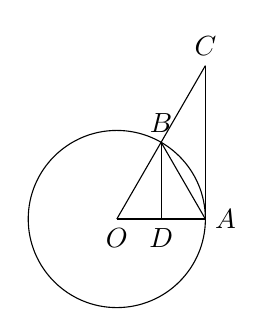
\begin{tikzpicture}[scale=1.125]
                \draw (0,0) circle (1);
                \filldraw[black] (0,0) node[below]{$O$};
                \draw[black](0,0) -- (1,0) node[right]{$A$};
                \draw[black](0,0) -- (1/2,{sqrt(3)/2}) node[above]{$B$};
                \draw[black](1/2,{sqrt(3)/2}) -- (1/2,0) node[below]{$D$};
                \draw[black](1,0) -- (1,{sqrt(3)}) node[above]{$C$};
                \draw[black](1,0) -- (1/2,{sqrt(3)/2});
                \draw[black](1,{sqrt(3)}) -- (1/2,{sqrt(3)/2});
            \end{tikzpicture}
        \end{minipage}

        根据图,在$x\in[0,\dfrac{\pi}{2}]$,$\sin x<x<\tan x$。

        $\therefore 1<\dfrac{x}{\sin x}<\dfrac{1}{\cos x}\Rightarrow\cos x<\dfrac{\sin x}{x}<1$。

        $\therefore 0<1-\dfrac{\sin x}{x}<1-\cos x=2\sin^2\dfrac{x}{2}\leqslant 2\left(\dfrac{x}{2}\right)^2$。

        根据夹逼定理,$\lim\limits_{x\to 0}2\left(\dfrac{x}{2}\right)^2=0\Rightarrow\lim\limits_{x\to 0}1-\dfrac{\sin x}{x}=0$。

        $\therefore\lim\limits_{x\to 0}\dfrac{\sin x}{x}=1$。

        从而$\lim\limits_{\Delta\to 0}\dfrac{\sin\Delta}{\Delta}=1(\Delta\neq 0)$。

        \subsection{\texorpdfstring{$\lim\limits_{x\to\infty}\left(1+\dfrac{1}{x}\right)^x=e$}{}}

        书上通过数列进行单调有界定理证明极限存在性。

        证明:$\lim\limits_{x\to\infty}\left(1+\dfrac{1}{x}\right)^x=\lim\limits_{x\to\infty}e^{\ln(1+\frac{1}{x})^x}=\lim\limits_{x\to\infty}e^{x\ln(1+\frac{1}{x})}=e^{\lim\limits_{x\to\infty}x\ln(1+\frac{1}{x})}=e^{\lim\limits_{x\to\infty}\frac{\ln(1+\frac{1}{x})}{\frac{1}{x}}}$

        $=e^{\lim\limits_{x\to\infty}\frac{\left(\frac{1}{1+\frac{1}{x}}\right)\cdot\left(-\frac{1}{x^2}\right)}{-\frac{1}{x^2}}}=e^{\lim\limits_{x\to\infty}\frac{1}{1+x}}=e$\medskip

        从而$\lim\limits_{\Delta\to\infty}\left(1+\dfrac{1}{\Delta}\right)^\Delta=e$与$\lim\limits_{\Delta\to 0}\left(1+\Delta\right)^{\frac{1}{\Delta}}=e(\Delta\neq 0)$。

        \section{无穷大与无穷小}

        \subsection{无穷}

        \subsubsection{无穷定义}

        无穷小\textcolor{violet}{\textbf{定义:}}当$x\to x_0(\infty)$时,函数$f(x)$极限为0,就称$f(x)$为当$x\to x_0(\infty)$时的无穷小,记为:$\lim\limits_{x\to x_0(\infty)}f(x)=0$。

        以0为极限的数列称为$n\to\infty$时的无穷小。

        无穷小是变量,不能与很小的数相等。

        零可以作为无穷小的唯一的数。

        \textcolor{aqua}{\textbf{定理:}}$\lim f(x)=A\Leftrightarrow f(x)=A+o(x)$,其中$\lim o(x)=0$。

        无穷大\textcolor{violet}{\textbf{定义:}}当$x\to x_0(\infty)$时,函数$\vert f(x)\vert$无限增大,就称$f(x)$为当$x\to x_0(\infty)$时的无穷大,记为:$\lim\limits_{x\to x_0(\infty)}f(x)=\infty$。

        若$\lim\limits_{x\to x_0}f(x)=\infty$则$x=x_0$为$y=f(x)$的垂直渐进线。

        若$\lim\limits_{x\to\infty}f(x)=a$则$y=a$为$y=f(x)$的水平渐进线。

        \textcolor{aqua}{\textbf{定理:}}若同一极限过程中,$f(x)$为无穷大,则$\dfrac{1}{f(x)}$为无穷小,反之若$f(x)$为无穷小且不为0,则$\dfrac{1}{f(x)}$为无穷大。

        \subsubsection{无穷小的比较}

        设在自变量同一变化过程中,$\lim\alpha(x)=0$,$\lim\beta(x)=0$,且$\beta(x)\neq 0$,则:

        \begin{enumerate}
            \item 若$\lim\dfrac{\alpha(x)}{\beta(x)}=0$,则$\alpha(x)$是比$\beta(x)$高阶的无穷小,记为$\alpha(x)=o(\beta(x))$。
            \item 若$\lim\dfrac{\alpha(x)}{\beta(x)}=\infty$,则$\alpha(x)$是比$\beta(x)$低阶的无穷小。
            \item 若$\lim\dfrac{\alpha(x)}{\beta(x)}=c\neq 0$,则$\alpha(x)$与$\beta(x)$是同阶无穷小。
            \item 若$\lim\dfrac{\alpha(x)}{\beta(x)}=1$,则$\alpha(x)$与$\beta(x)$是等价无穷小,记为$\alpha(x)\sim\beta(x)$。
            \item 若$\lim\dfrac{\alpha(x)}{[\beta(x)]^k}=c\neq 0$,则$\alpha(x)$是$\beta(x)$的$k$阶无穷小。
        \end{enumerate}

        \textcolor{aqua}{\textbf{定理:}}$\alpha(x)\sim\beta(x)$的充要条件是$\alpha(x)=\beta(x)+o(\beta(x))$。

        \textcolor{orange}{注意:}并不是任意无穷小都可以比阶。如$\lim\limits_{x\to 0}\dfrac{x\sin\dfrac{1}{x}}{x^2}$就因为得到函数振荡而无法得到极限。

        \textbf{例题:}证明当$x\to 0$时,$\sqrt[n]{1+x}-1\sim\dfrac{1}{n}x$。

        证明:证明$\sqrt[n]{1+x}-1\sim\dfrac{1}{n}x$就是证明$\lim\limits_{x\to 0}\dfrac{\sqrt[n]{1+x}-1}{x}\sim\dfrac{1}{n}$。

        令$\sqrt[n]{1+x}-1=t$,则$1+x=(1+t)^n$,则$x=(1+t)^n-1$。

        利用二项式展开:$=\lim\limits_{t\to 0}\dfrac{t}{nt+\dfrac{n(n-1)}{2}t^2+\cdots}=\dfrac{1}{n}$。

        \subsubsection{无穷小运算}

        设$m$,$n$为正整数:

        \begin{enumerate}
            \item $o(x^m)\pm o(x^n)=o(x^l),l=\min{m,n}$(加减法低阶吸收高阶)。
            \item $o(x^m)\cdot o(x^n)=o(x^{m+n}),x^m\cdot o(x^n)=o(x^{m+n})$(乘法累加)。
            \item $o(x^m)=o(k\cdot x^m)=k\cdot o(x^m)$,$k\neq 0$且为常数(非零常数相乘不影响阶数)。
        \end{enumerate}

        \subsection{洛必达法则}

        洛必达法则用于计算无穷的比值的极限,如$\dfrac{0}{0}$型和$\dfrac{\infty}{\infty}$型,如果趋向不同则不能使用。

        \textcolor{aqua}{\textbf{定理:}}当$x\to a$或$x\to\infty$时,函数$f(x)$以及$F(x)$都趋于零,$f'(x)$、$F'(x)$在点$a$的某去心邻域内(或当$\vert x\vert>X$,$X$为充分大的正数)存在,且$F'(x)\neq0$,$\lim\limits_{x\to a}\dfrac{f'(x)}{F'(x)}$或$\lim\limits_{x\to\infty}\dfrac{f'(x)}{F'(x)}$存在或无穷大时,则$\lim\limits_{x\to a}\dfrac{f(x)}{F(x)}=\lim\limits_{x\to a}\dfrac{f'(x)}{F'(x)}$或$\lim\limits_{x\to\infty}\dfrac{f(x)}{F(x)}=\lim\limits_{x\to\infty}\dfrac{f'(x)}{F'(x)}$。

        \textcolor{aqua}{\textbf{定理:}}当$x\to a$或$x\to\infty$时,函数$f(x)$以及$F(x)$都趋于无穷,$f'(x)$、$F'(x)$在点$a$的某去心邻域内(或当$\vert x\vert>X$,$X$为充分大的正数)存在,且$F'(x)\neq0$,$\lim\limits_{x\to a}\dfrac{f'(x)}{F'(x)}$或$\lim\limits_{x\to\infty}\dfrac{f'(x)}{F'(x)}$存在或无穷大时,则$\lim\limits_{x\to a}\dfrac{f(x)}{F(x)}=\lim\limits_{x\to a}\dfrac{f'(x)}{F'(x)}$或$\lim\limits_{x\to\infty}\dfrac{f(x)}{F(x)}=\lim\limits_{x\to\infty}\dfrac{f'(x)}{F'(x)}$。

        同理如果导数存在也可以不断求导:$\lim\limits_{x\to a}\dfrac{f(x)}{F(x)}=\lim\limits_{x\to a}\dfrac{f(x)'}{F(x)'}=\lim\limits_{x\to a}\dfrac{f(x)''}{F(x)''}$。

        \textcolor{orange}{注意:}洛必达法则求不出值也不能说其左边的值不存在。如$\lim\limits_{x\to0}\dfrac{x^2\sin\dfrac{1}{x}}{x}=\lim\limits_{x\to0}\sin\dfrac{1}{x}=0$,通过洛必达就求不出值。

        \subsection{泰勒公式}

        与洛必达法则不同,适用于$\dfrac{A}{B}$上下同阶型和$A-B$幂次最低型。如$\dfrac{x-\sin x}{x^3}$和$\cos x-e^{-\frac{x^2}{2}}$。

        是一个用函数在某点的信息描述其附近取值的公式。如果函数满足一定的条件,泰勒公式可以用函数在某一点的各阶导数值做系数构建一个多项式来近似表达这个函数,即用多项式拟合不规则曲线。

        \subsubsection{麦克劳林公式}

        \begin{enumerate}
            \item $e^x=\sum\limits_{i=0}^n\dfrac{1}{i!}x^i$,$=1+\dfrac{1}{1!}x+\dfrac{1}{2!}x^2+\dfrac{1}{3!}x^3+o(x^3)$。
            \item $\ln(1+x)=\sum\limits_{i=1}^n(-1)^{i+1}\dfrac{1}{i}x^i$,$=x-\dfrac{1}{2}x^2+\dfrac{1}{3}x^3+o(x^3)$。
            \item $\sin x=\sum\limits_{i=1}^{2i-1}(-1)^{2i-1}\dfrac{1}{(2i-1)!}x^{2i-1}$,$=x-\dfrac{1}{3!}x^3+\dfrac{1}{5!}x^5+o(x^5)$。
            \item $\cos x=\sum\limits_{i=1}^{2i}(-1)^{2i-1}\dfrac{1}{(2i-2)!}x^{2i-2}$,$=x-\dfrac{1}{2!}x^2+\dfrac{1}{4!}x^4+o(x^4)$。
            \item $\arcsin x=\sum\limits_{i=1}^{2i-1}\dfrac{(2i-3)!!}{(2i-2)!!}\dfrac{x^{2i-1}}{2i-1}$,$=x+\dfrac{1}{2}\dfrac{x^3}{3}+\dfrac{1\times3}{2\times4}\dfrac{x^5}{5}+\dfrac{1\times3\time5}{2\times4\times6}\dfrac{x^7}{7}+o(x^7)$。(假定$-1!=0!$)
            \item $\dfrac{1}{1-x}=\sum\limits_{i=0}^nx^i$,$=1+x+x^2+x^3+o(x^3)$。
            \item $(1+x)^a=1+\sum\limits_{i=1}^n\dfrac{\prod_{j=1}^i(a-j+1)}{i!}x^i$,$=1+\dfrac{a}{1!}x+\dfrac{a(a-1)}{2!}x^2\\+\dfrac{a(a-1)(a-2)}{3!}x^3+o(x^3)$。
        \end{enumerate}

        \subsubsection{常用等价无穷小}

        \textcolor{aqua}{\textbf{定理:}}若$\alpha\sim\alpha_1$,$\beta\sim\beta_1$,则$\lim\dfrac{\alpha}{\beta}=\lim\dfrac{\alpha_1}{\beta}=\lim\dfrac{\alpha}{\beta_1}=\lim\dfrac{\alpha_1}{\beta_1}$。

        所以可以使用等价无穷小替换对应式子,这些等价无穷小都是使用泰勒展开得到的。等价无穷小只是泰勒公式在某个固定阶数上(通常为一阶)的特例。

        通过麦克劳林公式可以得到当$x\to 0$时的相应等价无穷小:

        \begin{enumerate}
            \item $x\sim\sin x\sim\tan x\sim\arcsin x\sim\arctan x\sim\ln(1+x)\sim\ln(x+\sqrt{1+x^2})\sim e^x-1$。
            \item $a^x-1\sim x\ln a$。
            \item $(1+x)^a-1\sim ax$。
            \item $\log_a(1+x)\sim\dfrac{x}{\ln a}$。
            \item $1-\cos x\sim\dfrac{1}{2}x^2$。
            \item $x-\ln(1+x)\sim\dfrac{1}{2}x^2$。
            \item $x-\sin x\sim\dfrac{1}{6}x^3$。
            \item $\arcsin x-x\sim\dfrac{1}{6}x^3$。
            \item $\tan x-x\sim\dfrac{1}{3}x^3$。
            \item $x-\arctan x\sim\dfrac{1}{3}x^3$。
            \item $\tan x-\sin x\sim\dfrac{1}{2}x^3$
        \end{enumerate}

        \subsubsection{等价无穷小适用性}

        如果是乘除关系可以随便换,但是加减关系需要一定条件:

        \begin{itemize}
            \item 若$\alpha\sim\alpha_1$,$\beta\sim\beta_1$,且$\lim\dfrac{\alpha_1}{\beta 1}=A\neq1$,则$\alpha-\beta\sim\alpha_1-\beta_1$。
            \item 若$\alpha\sim\alpha_1$,$\beta\sim\beta_1$,且$\lim\dfrac{\alpha_1}{\beta 1}=A\neq-1$,则$\alpha+\beta\sim\alpha_1+\beta_1$。
        \end{itemize}

        即这两个和不能为0。

        \section{函数连续性与间断点}

        函数的连续与间断是逐点的概念。

        \subsection{连续定义}

        \textcolor{violet}{\textbf{定义:}}若函数$f(x)$在点$x_0$的某一邻域内有定义,且有$\lim\limits_{x\to x_0}f(x)=f(x_0)$或$\lim\limits_{\Delta x\to 0}\Delta y=0$,则称函数$f(x)$在点$x_0$处连续。

        极限值等于函数值,则该点连续。

        在区间上每一点都连续的函数,就是该区间上的连续函数,或该函数在该区间上连续。

        \subsection{间断定义}

        讨论间断只看两类点:分段函数分段点,无定义点。

        \textcolor{violet}{\textbf{定义:}}若函数$f(x)$在点$x_0$的某一去心邻域内有定义,且有$\lim\limits_{x\to x_0}f(x)\neq f(x_0)$,则称函数$f(x)$在点$x_0$处间断。

        极限值不等于函数值,则该点间断。

        \subsection{间断点分类}

        \subsubsection{可去间断点(可补间断点)}

        \begin{minipage}{0.6\linewidth}
            \textcolor{violet}{\textbf{定义:}}若$\lim\limits_{x\to x_0}f(x)=A\neq f(x_0)$(甚至可以没有定义)。
        \end{minipage}
        \hfill
        \begin{minipage}{0.3\linewidth}
            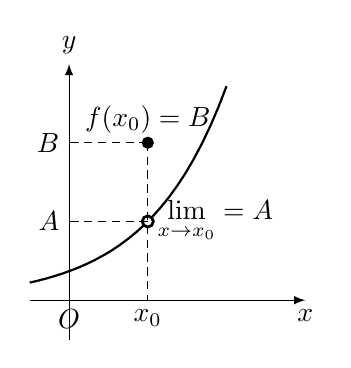
\begin{tikzpicture}
                \draw[-latex](-0.5,0) -- (3,0) node[below]{$x$};
                \draw[-latex](0,-0.5) -- (0,3) node[above]{$y$};
                \filldraw[black] (0,0) node[below]{$O$};
                \draw[black, thick, domain=-0.5:2] plot (\x,{pow(e,\x-1)});
                \filldraw[white, draw=black, line width=1pt] (1,1) circle (2pt);
                \draw[black, densely dashed](1,2) -- (0,2) node[left]{$B$};
                \draw[black, densely dashed](1,1) -- (0,1) node[left]{$A$};
                \draw[black, densely dashed](1,2) -- (1,0) node[below]{$x_0$};
                \filldraw[black] (1,2) circle (2pt) node[above]{$f(x_0)=B$};
                \filldraw[black] (1,1) node[right]{$\lim\limits_{x\to x_0}=A$};
            \end{tikzpicture}
        \end{minipage}

        \subsubsection{跳跃间断点}

        \begin{minipage}{0.6\linewidth}
            \textcolor{violet}{\textbf{定义:}}若$\lim\limits_{x\to x_0^-}f(x)$与$\lim\limits_{x\to x_0^+}f(x)$都存在,但是$\lim\limits_{x\to x_0^-}f(x)\neq\lim\limits_{x\to x_0^+}f(x)$。
        \end{minipage}
        \hfill
        \begin{minipage}{0.3\linewidth}
            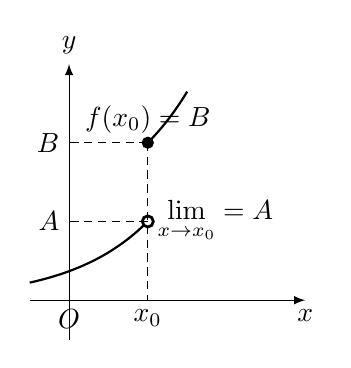
\begin{tikzpicture}
                \draw[-latex](-0.5,0) -- (3,0) node[below]{$x$};
                \draw[-latex](0,-0.5) -- (0,3) node[above]{$y$};
                \filldraw[black] (0,0) node[below]{$O$};
                \draw[black, thick, domain=-0.5:1] plot (\x,{pow(e,\x-1)});
                \draw[black, thick, domain=1:1.5] plot (\x,{pow(e,\x-1)+1});
                \filldraw[white, draw=black, line width=1pt] (1,1) circle (2pt);
                \draw[black, densely dashed](1,2) -- (0,2) node[left]{$B$};
                \draw[black, densely dashed](1,1) -- (0,1) node[left]{$A$};
                \draw[black, densely dashed](1,2) -- (1,0) node[below]{$x_0$};
                \filldraw[black] (1,2) circle (2pt) node[above]{$f(x_0)=B$};
                \filldraw[black] (1,1) node[right]{$\lim\limits_{x\to x_0}=A$};
            \end{tikzpicture}
        \end{minipage} \medskip

        可去间断点与跳跃间断点的左右极限都存在的间断点都称为第一类间断点。

        \subsubsection{无穷间断点}

        \begin{minipage}{0.6\linewidth}
            \textcolor{violet}{\textbf{定义:}}若$\lim\limits_{x\to x_0}f(x)=\infty$,或至少一个方向为无穷大(定义分歧)。如$y=\dfrac{1}{x}$在$x=0$处为无穷间断点。
        \end{minipage}
        \hfill
        \begin{minipage}{0.3\linewidth}
            \begin{tikzpicture}
                \draw[-latex](-2,0) -- (2,0) node[below]{$x$};
                \draw[-latex](0,-2) -- (0,2) node[above]{$y$};
                \filldraw[black] (0,0) node[below]{$O$};
                \draw[black, thick, domain=0.5:2] plot (\x,{pow(\x,-1)});
                \draw[black, thick, domain=-2:-0.5] plot (\x,{pow(\x,-1)});
            \end{tikzpicture}
        \end{minipage}

        \subsubsection{振荡间断点}

        \begin{minipage}{0.6\linewidth}
            \textcolor{violet}{\textbf{定义:}}若$\lim\limits_{x\to x_0}f(x)$为振荡不存在。如$\lim\limits_{x\to 0}\sin\dfrac{1}{x}$的$x=0$就是振荡间断点。
        \end{minipage}
        \hfill
        \begin{minipage}{0.3\linewidth}
            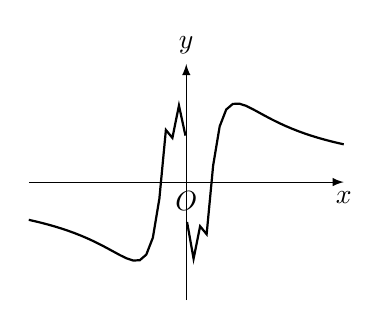
\begin{tikzpicture}
                \draw[-latex](-2,0) -- (2,0) node[below]{$x$};
                \draw[-latex](0,-1.5) -- (0,1.5) node[above]{$y$};
                \filldraw[black] (0,0) node[below]{$O$};
                \draw[black, thick, domain=0.01:2] plot (\x,{sin(pow(\x,-1) r)});
                \draw[black, thick, domain=-2:-0.01] plot (\x,{sin(pow(\x,-1) r)});
            \end{tikzpicture}
        \end{minipage}

        无穷间断点与振荡间断点的左右极限都不存在的点都是第二类间断点。

        \textcolor{orange}{注意:}两侧邻域都有定义才能讨论间断点问题。\medskip

        \textbf{例题:}若$f(x)=\left\{
        \begin{array}{lcl}
            2x+a, & & x\leqslant 0 \\
            e^x(\sin x+\cos x), & & x>0
        \end{array} \right.
        $在$(-\infty,+\infty)$内连续,求$a$。

        解:因为连续,所以$f(0)=\lim\limits_{x\to 0^+}f(x)=\lim\limits_{x\to 0^-}f(x)$。

        $\therefore a=1$。

        \textbf{例题:}若函数$f(x)=\dfrac{\ln\vert x\vert}{\vert x-1\vert}\sin x$,则x的间断点类型是?\medskip

        解:由式子的分式部分可知有两个无定义的间断点:$x=0$,$x=1$。\medskip

        $\lim\limits_{x\to 1}f(x)=\lim\limits_{x\to 1}\dfrac{x-1}{\vert x-1\vert}\sin x=\left\{
        \begin{array}{lcl}
            x\to 1^+ & \rightarrow & \sin 1 \\
            x\to 1^- & \rightarrow & -\sin 1
        \end{array} \right.
        $。

        所以$x=1$跳跃间断点。

        $\lim\limits_{x\to 0}f(x)=\lim\limits_{x\to 0}\ln\vert x\vert\cdot\sin x=\lim\limits_{x\to 0}x\ln\vert x\vert=0$。

        而$x=0$未定义,所以其为可去间断点。

        \subsection{函数连续性}

        \subsubsection{连续函数四则运算的连续性}

        若两个函数在某点连续,则这两个函数的和差积商在该点都连续。但是如果两个在某点不连续的函数,其和差积商在某点的连续性都是不一定的,所以反过来,如果一个函数的和差积商是在某点连续的,不能说明这个组成的多个函数在该点是连续的。

        \subsubsection{反函数的连续性}

        若函数在定义域是严格单调的函数,则其反函数在其原值域上也是连续的且单调性不变。

        \subsubsection{复合函数的连续性}

        若$y=f(g(x))$由$y=f(u)$与$u=g(x)$复合而成,若$g(x)$在$x_0$处连续,$f(u)$在$u_0$处连续,且$u_0=g(x_0)$,则$f(g(x))$在$x_0$处连续。

        \subsubsection{初等函数的连续性}

        基本初等函数在定义域上是连续的。

        初等函数在定义区间上是连续的。

        定义区间是定义域的子集。

        \section{闭区间上连续函数的性质}

        设$f(x)$在区间$[a,b]$上连续,则:

        \subsection{有界性与最大最小值定理}

        最大最小值\textcolor{aqua}{\textbf{定理:}}:$f(x)$在$[a,b]$上必有最大值和最小值。

        有界性\textcolor{aqua}{\textbf{定理:}}$f(x)$在$[a,b]$上必有界。

        如果是开区间连续则不能保证有界性,因为可能开区间两边的端点为函数的间断点(如$\dfrac{1}{x}$在$x=0$处)。

        \subsection{零点与介值定理}

        零点\textcolor{aqua}{\textbf{定理:}}若$f(a)f(b)<0$,则$\exists\,\xi\in[a,b]$使得$f(\xi)=0$。

        介值\textcolor{aqua}{\textbf{定理:}}若$f(a)\neq f(b)$,$\mu$为介于$f(a)$与$f(b)$之间的任何值,那么至少存在$\xi\in[a,b]$使得$f(\xi)=\mu$。

        \textbf{例题:}证明方程$x=a\sin x+b(a>0,b>0)$中至少有一个正根,并且不超过$a+b$。

        证明:令$f(x)=x-a\sin x-b$,其中$f(0)=-b<0$,$f(a+b)=a+b=a\sin(a+b)-b=a[1-\sin(a+b)]\geqslant 0$。

        若$\sin(a+b)=1$,则根为$a$,结论成立。

        若$\sin(a+b)<1$,$\because f(a+b)\cdot f(0)<0$根据零点定理$\exists\,\xi\in[0,a+b]$使得$f(\xi)=0$,从而得证。

        \subsection{*一致连续性}

        \textcolor{violet}{\textbf{定义:}}设函数$f(x)$在区间$I$上有定义,若对于任意给定的正数$\xi$,总存在正数$\delta$,使得对于区间$I$上的任意两点$x_1x_2$,当$\vert x_1-x_2\vert<\delta$时,有$\vert f(x_1)-f(x_2)\vert<\xi$,则函数$f(x)$在区间$I$上一致连续。

        对于连续性的定义:设函数$f(x)$在区间$I$上有定义,若对于任意给定的正数$\xi$,总存在正数$\delta$,使得对于区间$I$上的任意一点$x$,当$\vert x-x_0\vert<\delta$时,有$\vert f(x)-f(x_0)\vert<\xi$,则称函数$f(x)$在区间$I$上连续。

        对比连续性与一致连续性,可以知道定义上就只有一个差别,连续性只有一个动点$x$($x_0$会相对于$x$而变化),而一致连续性有两个动点$x_1x_2$。但是就是这种小变化会带来很大不同的定义结果。

        可以利用几何图形来分析,对于图像上的任意一点,连续性与一致连续性都是在一个过程中固定一个$\xi$,来求对应的$\delta$。所导致的就是函数差值是固定的。

        根据连续定义,函数上任意取一个$x$,再在$x$的左边或右边取一个$x_0$,使得$\vert f(x)-f(x_0)\vert<\xi$,现在需要求一个$\delta$,使得$\delta$,使得$\vert x-x_0\vert<\delta$,所以我们可以根据这个条件,作一个竖直距离为$\xi$,水平距离为$\delta$的长方形,长方形内部的所有点的$x$坐标代表的$\delta$都满足条件,其中一个正对角点坐标为$(x,f(x))$,另一个则为$(x_0,f(x_0))$。$\xi$是固定的,要根据不同的$x$找到不同的$\delta$,即不同的$x+\delta=x_0$。

        假定函数为$y=\dfrac{1}{x}$,$\xi=1$,任意取一点$x$,求出对应的$\delta$,将会得到下面第一张图。其中虚线里的所有点都是满足要求的点。而随着$x$上移,长方形水平长度会无限接近于0,而向下,长方形水平长度会无限接近于$+\infty$。

        \begin{tikzpicture}[scale=1]
            \draw[-latex](-0.5,0) -- (5,0) node[below]{$x$};
            \draw[-latex](0,-0.5) -- (0,5) node[above]{$y$};
            \filldraw[black] (0,0) node[below]{$O$};
            \draw[black, densely dashed](1,2) -- (1,1) node[right]{$x$};
            \draw[black, densely dashed](1/2,1) -- (1/2,2);
            \draw[black, densely dashed](1,2) -- (1/2,2) node[left]{$x_0$};
            \draw[black, densely dashed](1,1) -- (1/2,1);
            \draw[black, thick, smooth, domain=0.2:5] plot (\x,{pow(\x,-1)});
        \end{tikzpicture}
        \begin{tikzpicture}[scale=1]
            \draw[-latex](-0.5,0) -- (5,0) node[below]{$x$};
            \draw[-latex](0,-0.5) -- (0,5) node[above]{$y$};
            \filldraw[black] (0,0) node[below]{$O$};
            \draw[black, densely dashed](1,2) -- (1,1);
            \draw[black, densely dashed](1/2,1) -- (1/2,2);
            \draw[black, densely dashed](1,2) -- (1/2,2);
            \draw[black, densely dashed](1,1) -- (1/2,1);
            \draw[black, thick, smooth, domain=0.25:5] plot (\x,{pow(\x,-1)+1});
            \draw[black, thick, smooth, domain=0.175:1] plot (\x,{pow(\x,-1)-1});
            \filldraw[white, draw=black, line width=1pt] (1,0) circle (2pt) ;
            \filldraw[black] (1.25,0.5) node{$\dfrac{1}{\xi}$};
        \end{tikzpicture}

        所以长方形的两对角点变动轨迹如图二所示,当$x$无限接近$+\infty$时,$x_0$无限接近$\dfrac{1}{\xi}$,因为$\lim\limits_{x\to+\infty}\dfrac{1}{\dfrac{1}{x}+\xi}=\dfrac{1}{\xi}$。

        所以连续性下总能找到一个$\delta$使得虚线长方形存在,从而函数$\dfrac{1}{x}$是具有连续性的。

        而对于连续一致性,则规定了两个变量$x_1x_2$,其实对比连续性类似,但是这时候虚线长方形的两个角都是被约束的,而不是连续性的时候$x_0$是不受约束的,对应到图形上,就是要找到一个长方形,使得无论$x_1x_2$在哪里都在长方形中。

        而对于函数$\dfrac{1}{x}$,由图像二可知虚线长方形的面积是从0一直变大到$+\infty$,所以不存在一个固定的长方形(面积为常数)。从而该函数不具有一致连续性。

        所以综上只有变化率变化不大的函数才在\textbf{整个定义域}上具有一致连续性。如一次线性函数,$\sin x$,$\cos x$,而对数函数,指数函数都不具有一致连续性。

        \textcolor{aqua}{\textbf{定理:}}若函数在闭区间上连续,则一定在该区间上一致连续。

        \textcolor{aqua}{\textbf{定理:}}若函数在某区间上一致连续,则一定在该区间上连续。

        \section{导数概念}
        \subsection{引例}

        设$f(x)$下$x$在$x_0$的邻域内,$\alpha$为切线所成夹角。

        $\tan\alpha=f'(x_0)=\lim\limits_{x\to x_0}\dfrac{f(x)-f(x_0)}{x-x_0}=k$。

        导数的本质是增量比的极限。

        \subsection{定义}

        设$y=f(x)$定义在区间$I$上,让自变量在$x=x_0$处加一个增量$\Delta x$,其中$x_0\in I$,$x_0+\Delta x\in I$,则可得函数的增量$\Delta y=f(x_0+\Delta x)-f(x_0)$。若函数增量$\Delta y$与自变量增量$\Delta x$的比值在$\Delta x\to 0$时的极限存在,则称函数$y=f(x)$在$x_0$处可导,并称这个极限为$y=f(x)$在点$x_0$处的导数,记作$f'(x)$,即$f'(x)=\lim\limits_{\Delta x\to 0}\dfrac{\Delta y}{\Delta x}=\lim\limits_{\Delta x\to 0}\dfrac{f(x_0+\Delta x)-f(x_0)}{\Delta x}$。\medskip

        下面三句话等价:

        \begin{enumerate}
            \item $y=f(x)$在$x_0$处可导。
            \item $y=f(x)$在$x_0$处导数存在。
            \item $f'(x)=A$。($A$为有限数)
        \end{enumerate}

        单侧导数分为左导数和右导数。\medskip

        $f'_-(x)=\lim\limits_{\Delta x\to 0^-}\dfrac{\Delta y}{\Delta x}=\lim\limits_{\Delta x\to 0}\dfrac{f(x_0+\Delta x)-f(x_0)}{\Delta x}$

        $f'_+(x)=\lim\limits_{\Delta x\to 0^+}\dfrac{\Delta y}{\Delta x}=\lim\limits_{\Delta x\to 0}\dfrac{f(x_0+\Delta x)-f(x_0)}{\Delta x}$\medskip

        所以$f(x)$在$x_0$处可导的充要条件是其左导数和右导数存在且相等。

        若$f(x)$在$x_0$的左右,如$y=\vert x\vert$在$0$的左右出现了单侧的不同的切线,那这个$x_0$就是一个\textbf{角点},该角点处不可导。

        若$f(x)$在$x_0$处导数为无穷,如$y=x^{\frac{1}{3}}$在$0$处利用导数的极限定义计算得到为正无穷,那么该点的导数为无穷导数,在考研中被认为是不存在的。

        \textcolor{aqua}{\textbf{定理:}}若$f(x)$为可导的偶函数,则$f'(x)$为奇函数,若$f(x)$为可导的奇函数,则$f'(x)$为偶函数。

        该证明是准备部分的定理。

        证明:首先已知$f(-x)=f(x)$,证明$f'(-x)=-f'(x)$。

        $\therefore$

        $
        \begin{aligned}
            f'(-x) &=\lim\limits_{\Delta x\to 0}\dfrac{f(-x+\Delta x)-f(-x)}{\Delta x} \\
            & =\lim\limits_{\Delta x\to 0}\dfrac{f(x+(-\Delta x))}{\Delta x} \\
            & =-\lim\limits_{-\Delta x\to 0}\dfrac{f(x+(-\Delta x))}{-\Delta x} \\
            & =-f'(x)
        \end{aligned}
        $

        同理得证$f(-x)=-f(x)\Rightarrow f'(-x)=f'(x)$。

        \textcolor{aqua}{\textbf{定理:}}$f(x)$为可导的周期为$T$的周期函数,则$f'(x)$也是以$T$为周期的周期函数。

        证明:已知$f(x+T)=f(x)$,求证$f'(x+T)=f'(x)$。\medskip

        $\therefore f'(x+T)=\lim\limits_{\Delta x\to 0}\dfrac{f(x+T+\Delta x)-f(x+T)}{\Delta x}$

        $=\lim\limits_{\Delta x\to 0}\dfrac{f(x+\Delta x)-f(x)}{\Delta x}=f'(x)$。

        \textbf{例题:}设$f(x)$是二阶可导的以2为周期的奇函数,且$f(\dfrac{1}{2})>0$,$f'(\dfrac{1}{2})>0$,比较$f(-\dfrac{1}{2})$、$f'(\dfrac{3}{2})$、$f''(0)$的大小。\medskip

        解:$\because f(x)$为二阶奇函数,$\therefore f(x)\text{奇函数}\Rightarrow f'(x)\text{偶函数}\Rightarrow f''(x)\text{奇函数}\Rightarrow f''(0)=0$。

        $\therefore f(-\dfrac{1}{2})=-f(\dfrac{1}{2})<0$。

        $\because f(x)T=2\Rightarrow f'(x)T=2$,$\therefore f'(\dfrac{3}{2})=f'(\dfrac{3}{2}-2)=f'(-\dfrac{1}{2})=f'(\dfrac{1}{2})>0$。

        $\therefore f'(\dfrac{3}{2})>f''(0)>f(-\dfrac{1}{2})$。\medskip

        \textbf{例题:}$\left(x^\alpha\right)'=\alpha x^{\alpha-1}(x>0)$。\medskip

        解:$\lim\limits_{\Delta x\to 0}\dfrac{f(x+\Delta x)-f(x)}{\Delta x}=\lim\limits_{\Delta x\to 0}\dfrac{\left(x+\Delta x\right)^\alpha-x^\alpha}{\Delta x}$\medskip

        $=\lim\limits_{\Delta x\to 0}\dfrac{x^\alpha\left[\left(1+\dfrac{\Delta x}{x}\right)^\alpha-1\right]}{\Delta x}=\lim\limits_{\Delta x\to 0}\dfrac{x^\alpha\cdot\alpha\cdot\dfrac{\Delta x}{x}}{\Delta x}=\alpha x^{\alpha-1}$

        \subsection{导数的几何意义}

        导数$f'(x_0)$在几何上就是曲线$y=f(x)$在点$(x_0,f(x_0))$处切线的斜率。

        切线方程:$y-y_0=f'(x_0)(x-x_0)$。

        法线方程:$y-y_0=-\dfrac{1}{f'(x_0)}(x-x_0)$。

        \subsection{可导与连续的关系}

        \textcolor{aqua}{\textbf{定理:}}可导必连续,连续不一定可导。

        证明:已知连续定义:$\lim\limits_{\Delta x\to 0}f(x+\Delta x)=f(x)$,即$\lim\limits_{\Delta x\to 0}f(x+\Delta x)-f(x)=0$。

        可导定义:$f'(x)=\lim\limits_{\Delta x\to 0}\dfrac{f(x+\Delta x)-f(x)}{\Delta x} = A$

        $\lim\limits_{\Delta x\to 0}f(x+\Delta x)-f(x)=\lim\limits_{\Delta x\to 0}\dfrac{f(x+\Delta x)-f(x)}{\Delta x}\cdot\Delta x=A\cdot 0=0$

        \textcolor{aqua}{\textbf{定理:}}若$f(x)$在$x=x_0$处连续,且$\lim\limits_{x\to x_0}\dfrac{f(x)}{x-x_0}=A$,则$f(x_0)=0$且$f'(x_0)=A$。

        证明:$\because\text{连续,}\therefore f(x_0)=\lim\limits_{x\to x_0}f(x)=\lim\limits_{x\to x_0}\dfrac{f(x)}{x-x_0}(x-x_0)=A\cdot 0=0$。

        又$f'(x_0)=\lim\limits_{x\to x_0}\dfrac{f(x)-f(x_0)}{x-x_0}=\lim\limits_{x\to x_0}\dfrac{f(x)}{x-x_0}=A$。

        如$\lim\limits_{x\to 1}\dfrac{f(x)}{x-1}=2$且$f(x)$连续,可以推出$f(1)=0$与$f'(1)=2$。

        \section{函数求导法则}

        \subsection{四则运算}

        若函数可导:

        \begin{enumerate}
            \item 和差的导数:$[u(x)\pm v(x)]'=u'(x)\pm v'(x)$。
            \item 积的导数:$[u(x)v(x)]'=u'(x)v(x)+u(x)v'(x)$,\\ $[u(x)v(x)w(x)]'=u'(x)v(x)w(x)+u(x)v'(x)w(x)+u(x)v(x)w'(x)$。
            \item 商的导数:$\left[\dfrac{u(x)}{v(x)}\right]'=\dfrac{u'(x)v(x)-u(x)v'(x)}{[v(x)]^2}$,$v(x)\neq 0$。
        \end{enumerate}

        证明$(uv)'=u'v+uv'$。

        证明:令$f(x)=u(x)v(x)$。

        $(u\cdot v)'$

        $=f'(x)=\lim\limits_{\Delta x\to 0}\dfrac{f(x+\Delta x)-f(x)}{\Delta x}=\lim\limits_{\Delta x\to 0}\dfrac{u(x+\Delta x)v(x+\Delta x)-u(x)v(x)}{\Delta x}$

        $=\lim\limits_{\Delta x\to 0}\dfrac{u(x+\Delta x)v(x+\Delta x)-u(x)v(x+\Delta x)+u(x)v(x+\Delta x)-u(x)v(x)}{\Delta x}$

        $=\lim\limits_{\Delta x\to 0}\dfrac{u(x+\Delta x)-u(x)}{\Delta x}v(x+\Delta x) +\lim\limits_{\Delta x\to 0}\dfrac{v(x+\Delta x)-v(x)}{\Delta x}u(x)$

        $=u'(x)v(x)+v'(x)u(x)$

        \subsection{反函数导数}

        \textcolor{aqua}{\textbf{定理:}}$y=f(x)$可导,且$f'(x)\neq 0$,

        则存在反函数$x=\varphi(y)$,且$\dfrac{\textrm{d}x}{\textrm{d}y}=\dfrac{1}{\dfrac{\textrm{d}y}{\textrm{d}x}}$,即$\varphi'(x)=\dfrac{1}{f'(x)}$。\medskip

        $y=f(x)$可导,且$f'(x)\neq 0$就是指严格单调,而严格单调必有反函数。

        \textbf{例题:}求$y=\arcsin x,x\in(-1,1)$与$y=\arctan x$的导数。

        解:首先反三角函数就是三角函数的反函数。

        求$y=\arcsin x$,即$x=\sin y$。\medskip

        $\therefore\dfrac{\textrm{d}\arcsin x}{\textrm{d}x}=\dfrac{1}{\dfrac{\textrm{d}\sin y}{\textrm{d}y}}=\dfrac{1}{\cos y}=\dfrac{1}{\sqrt{1-\sin^2y}}=\dfrac{1}{\sqrt{1-x^2}}$。\medskip

        求$y=\arctan x$,就$x=\tan y$。\medskip

        $\therefore\dfrac{\textrm{d}\arctan x}{\textrm{d}x}=\dfrac{1}{\dfrac{\textrm{d}\tan y}{\textrm{d}y}}=\dfrac{1}{\sec^2y}=\dfrac{1}{1+\tan^2y}=\dfrac{1}{1+x^2}$。\medskip

        二阶反函数导数\textcolor{aqua}{\textbf{定理:}}:\medskip

        $f''(x)=y''_{xx}=\dfrac{\textrm{d}\left(\dfrac{\textrm{d}y}{\textrm{d}x}\right)}{\textrm{d}x}=\dfrac{\textrm{d}^2y}{\textrm{d}x^2}=\dfrac{\textrm{d}\left(\dfrac{1}{\varphi'(y)}\right)}{\textrm{d}x}=\dfrac{\textrm{d}\left(\dfrac{1}{\varphi'(y)}\right)}{\textrm{d}y}\cdot\dfrac{\textrm{d}y}{\textrm{d}x}$

        $=-\dfrac{x_{yy}''}{(x_y')^2}\cdot\dfrac{1}{x_y'}=-\dfrac{x_{yy}''}{(x_y')^3}$\medskip

        其中$\textrm{d}x\cdot\textrm{d}x=(\textrm{d}x)^2=\textrm{d}x^2$称为微分的幂,而$\textrm{d}(x^2)$叫幂的微分。

        \textbf{例题:}设$y=f(x)$的反函数是$x=\varphi(y)$,且$f(x)=\int_1^{2x}e^{t^2}\textrm{d}t+1$,求$\varphi''(1)$。

        解:$\because y=f(x)$,$\therefore x=\varphi(y)$,$x_{yy}''=\varphi''(y)=-\dfrac{y_{xx}''}{(y_x')^3}=-\dfrac{f''(x)}{[f'(x)]^3}$。\medskip

        其中根据变限积分求导公式:$f'(x)=2e^{4x^2}$,$f''(x)=2e^{4x^2}\cdot 8x=16xe^{4x^2}$。\medskip

        又$y=1\Rightarrow x=\dfrac{1}{2}\Rightarrow\varphi''(1)=-\dfrac{f''\left(\dfrac{1}{2}\right)}{\left[f'\left(\dfrac{1}{2}\right)\right]^3}=-\dfrac{1}{e^2}$。

        \subsection{复合函数的导数}

        \textcolor{aqua}{\textbf{定理:}}$u=g(x)$在$x$可导,$y=f(u)$在$u=g(x)$处可导,则$\{f[g(x)]\}'=f'[g(x)]g'(x)$。

        \textbf{例题:}设$f(x)=\prod\limits_{n=1}^{100}\left(\tan\dfrac{\pi x^n}{4}-n\right)$,则$f'(1)$为?

        解:原式=$\left(\tan\dfrac{\pi x}{4}-1\right)\left(\tan\dfrac{\pi x^2}{4}-2\right)\cdots\left(\tan\dfrac{\pi x^{100}}{4}-100\right)$。

        令$\left(\tan\dfrac{\pi x^2}{4}-2\right)\cdots\left(\tan\dfrac{\pi x^{100}}{4}-100\right)=g(x)$。\medskip

        $\therefore f(x)=\left(\tan\dfrac{\pi x}{4}-1\right)\cdot g(x)$。\medskip

        $\therefore f'(x)=\sec^2\dfrac{\pi x}{4}\cdot\dfrac{\pi}{4}\cdot g(x)+\left(\tan\dfrac{\pi x}{4}-1\right)\cdot g'(x)$。\medskip

        $\therefore$根据导数的四则运算,需要导数的乘积为每一项求导乘以其他不求导项的和,而$\tan\dfrac{\pi x}{4}-1$当$x=1$时为0,只要它不求导,其他的项都必然是0,所以原式的后面的结果都是0。

        $\therefore f'(1)$

        $=f'(x)\vert_{x=1}=\dfrac{\pi}{2}\cdot g(1)+0\cdot g'(x)=\dfrac{\pi}{2}\cdot g(1)=\dfrac{\pi}{2}(-1)(-2)\cdots(-99)=-\dfrac{\pi}{2}\cdot 99!$

        \subsection{分段函数的导数}

        设$f(x)=\left\{
        \begin{array}{lcl}
            f_1(x), & & x\geqslant x_0 \\
            f_2(x), & & x<x_0 \\
        \end{array}
        \right.$。\medskip

        在分段点用定义:

        判断$f'_+(x_0)=\lim\limits_{x\to x_0^+}\dfrac{f_1(x)-f(x_0)}{x-x_0}\overset{?}{=}\lim\limits_{x\to x_0^-}\dfrac{f_2(x)-f(x_0)}{x-x_0}$。如果相等就挖去这个点,否则就包含这个点。

        非分段点使用导数公式求导:$x>x_0,f'(x)=f_1'(x),x<0,f'(x)=f_2'(x)$。

        \subsection{对数求导法}

        对于多项相乘、相除、开方、乘方的式子,一般先取对数再求导,设$y=f(x)(f(x)>0)$,则\ding{172}等式两边取对数:$\ln y=\ln f(x)$。\ding{173}两边对自变量$x$求导,得$\dfrac{1}{y}y'=[\ln f(x)]'\Rightarrow y'=y[\ln f(x)]'$。

        \textbf{例题:}求$y=\sqrt[3]{\dfrac{(x+1)(2x-1)^2}{(4-3x)^5}}$的导数。

        解:取对数:$\ln\vert y\vert=\dfrac{1}{3}[\ln\vert x+1\vert+2\ln\vert 2x-1\vert-5\ln\vert 4-3x\vert]$。

        $\because \ln\vert y\vert'=\ln y'$。

        两边对x求导:\medskip

        $\dfrac{y'}{y}=\dfrac{1}{3}\left(\dfrac{1}{x+1}+\dfrac{4}{2x-1}-\dfrac{5}{4-3x}\cdot(-3)\right)$

        $\therefore y'=\dfrac{1}{3}\left(\dfrac{1}{x+1}+\dfrac{4}{2x-1}-\dfrac{5}{4-3x}\cdot(-3)\right)y$

        \subsection{幂指函数求导法}

        非常重要。

        对于$u(x)^{v(x)}(u(x)>0,u(x)\neq 1)$,除了对数求导法外还可以使用指数函数$u(x)^{v(x)}=e^{v(x)\ln u(x)}$。

        然后求导得到$[u(x)^{v(x)}]'=[e^{v(x)\ln u(x)}]'$

        $=u(x)^{v(x)}\left[v'(x)\ln u(x)+v(x)\cdot\dfrac{u'(x)}{u(x)}\right]$。

        \textbf{例题:}求$y=x^x(x>0)$的导数。

        解:$\because x^x=e^{x\ln x}$,$\therefore (x^x)'=(e^{x\ln x})'=x^x\cdot(\ln x+1)$。

        \textbf{例题:}求解$y=x^{\frac{1}{x}}(x>0)$的整数最大值。

        解:$\because y=x^{\frac{1}{x}}=e^{\frac{1}{x}\ln x}$。

        $\therefore y'=\left(x^{\frac{1}{x}}\right)=\left(e^{\frac{1}{x}\ln x}\right)'=x^{\frac{1}{x}}\cdot\dfrac{1-\ln x}{x^2}$。

        令导数结果为0,因为$x^{\frac{1}{x}}$与$x^2$在$x>0$时都不为0,所以只有一个驻点$x=e$。

        $0<x<e$时$1-\ln x$大于0,所以导数大于0,函数在该区间增。相反$x>e$时函数在区间减。

        研究驻点左侧情况,求对应的极限:$e^{\lim\limits_{x\to 0^+}\frac{\ln x}{x}}=e^{-\infty}\to 0$。

        研究驻点右侧情况,求对应的极限:$e^{\lim\limits_{x\to+\infty}\frac{\ln x}{x}}=e^0\to 1$。

        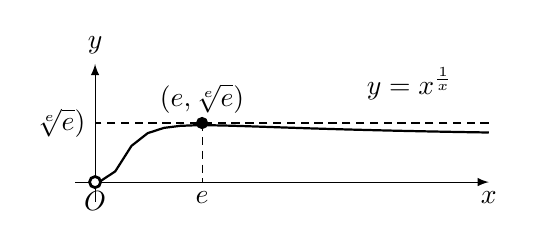
\begin{tikzpicture}[scale=0.5]
            \draw[-latex](-0.5,0) -- (10,0) node[below]{$x$};
            \draw[-latex](0,-0.5) -- (0,3) node[above]{$y$};
            \draw[black, thick, domain=0.1:10] plot (\x,{pow(\x,pow(\x,-1))});
            \filldraw[black] (8,2.5) node{$y=x^{\frac{1}{x}}$};
            \filldraw[white, draw=black, line width=1pt] (0,0) circle (4pt);
            \filldraw[black] (0,0) node[below]{$O$};
            \filldraw[black] (e,1.5) circle (4pt);
            \filldraw[black] (e,1.5) node[above]{$(e,\sqrt[e]{e})$};
            \draw[black, densely dashed](e,1.5) -- (e,0) node[below]{$e$};
            \draw[black, densely dashed](10,1.5) -- (0,1.5) node[left]{$\sqrt[e]{e})$};
        \end{tikzpicture}

        所以必然在$\sqrt{2}$与$\sqrt[3]{3}$两点取得整数最大值,而全部六次方后$\sqrt{2}^6=8<\sqrt[3]{3}=9$,所以$\sqrt[3]{3}$为最大整数解。

        \section{高阶导数}

        \subsection{定义}

        高阶导数\textcolor{violet}{\textbf{定义:}}$f^{(n)}(x_0)=\lim\limits_{\Delta x\to 0}\dfrac{f^{(n-1)}(x_0+\Delta x)-f^{(n-1)}(x_0)}{\Delta x}$,其中$n\geqslant 2$且$n\in N^+$,$f^{(n-1)}(x)$在$x_0$的某领域内有定义,$x_0+\Delta x$也在该邻域内。

        若$f^{(n)}(x)$在区间$I$上连续,称$f(x)$在$I$上$n$阶连续可导。

        \begin{itemize}
            \item $(e^x)^{(n)}=e^x$。
            \item $(\sin x)^{(n)}=\sin(x+n\dfrac{\pi}{2})$。
            \item $(\cos x)^{(n)}=\cos(x+n\dfrac{\pi}{2})$。
            \item $(\ln(1+x))^{(n)}=(-1)^{n-1}\dfrac{(n-1)!}{(1+x)^n}$。
        \end{itemize}

        \textcolor{aqua}{\textbf{定理:}}

        设$u,v$都是$n$阶可导,则:

        \begin{itemize}
            \item $(u\pm v)^{(n)}=u^{(n)}\pm v^{(n)}$。
            \item 莱布尼兹公式:$(uv)^{(n)}=\sum_{k=0}^nC_n^ku^{(n-k)}v^{(k)}$。
        \end{itemize}

        \subsection{归纳法}

        即依次求导得出规律。

        $(a^x)^n=a^x(\ln a)^{(n)}$,如$y=2^x$,则$y'=2^x\ln 2$,$y''=2^x(\ln 2)^2\cdots$得到$y^{(n)}=2^x(\ln 2)^n,n\in N$。

        \textbf{例题:}求$\sin x$的$n$阶导数。

        解:$\because \sin x'=\cos x$而不断求导会发现正负号会++--++--地变化而难以归纳为公式,所以需要另想办法。

        使用诱导公式:

        $y'=\cos x=\sin(x+\dfrac{\pi}{2})$

        $y''=\cos(x+\dfrac{\pi}{2})=\sin(x+\dfrac{\pi}{2}+\dfrac{\pi}{2})$

        $\cdots$

        $y^{(n)}=\sin(x+\dfrac{\pi}{2}\cdot n)$

        \subsection{莱布尼茨公式}

        \textcolor{violet}{\textbf{定义:}}设$u=u(x)$,$v=v(x)$均$n$阶可导,则$(uv)^{(n)}=\sum_{k=0}^nC_n^ku^{(n-k)}v^{(k)}$。

        展开:$(uv)^{(n)}=C_n^0u^{(n)}v^{(0)}+C_n^1u^{(n-1)}v'+\cdots+C_n^nu^{(0)}v^{(n)}$。

        莱布尼兹公式里的系数与考研数学准备章节的因式分解公式的二次项公式的系数一致,可以使用杨辉三角形来记忆:

        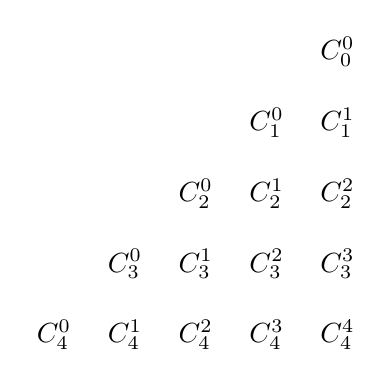
\begin{tikzpicture}[scale=0.9]
            \node[black] at (0,0) {$C_0^0$};
            \node[black] at (-1,-1) {$C_1^0$};
            \node[black] at (0,-1) {$C_1^1$};
            \node[black] at (-2,-2) {$C_2^0$};
            \node[black] at (-1,-2) {$C_2^1$};
            \node[black] at (-0,-2) {$C_2^2$};
            \node[black] at (-3,-3) {$C_3^0$};
            \node[black] at (-2,-3) {$C_3^1$};
            \node[black] at (-1,-3) {$C_3^2$};
            \node[black] at (-0,-3) {$C_3^3$};
            \node[black] at (-4,-4) {$C_4^0$};
            \node[black] at (-3,-4) {$C_4^1$};
            \node[black] at (-2,-4) {$C_4^2$};
            \node[black] at (-1,-4) {$C_4^3$};
            \node[black] at (-0,-4) {$C_4^4$};
        \end{tikzpicture}
        \hspace{2.5em}
        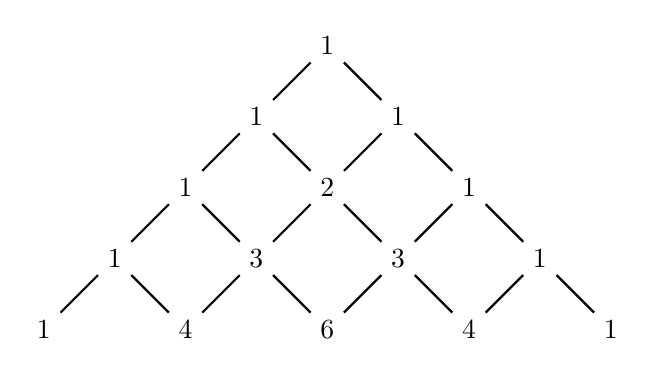
\begin{tikzpicture}[scale=0.9]
            \node[black] (0) at (0,0) {1};
            \node[black] (1) at (-1,-1) {1};
            \node[black] (2) at (1,-1) {1};
            \node[black] (3) at (-2,-2) {1};
            \node[black] (4) at (0,-2) {2};
            \node[black] (5) at (2,-2) {1};
            \node[black] (6) at (-3,-3) {1};
            \node[black] (7) at (-1,-3) {3};
            \node[black] (8) at (1,-3) {3};
            \node[black] (9) at (3,-3) {1};
            \node[black] (10) at (-4,-4) {1};
            \node[black] (11) at (-2,-4) {4};
            \node[black] (12) at (0,-4) {6};
            \node[black] (13) at (2,-4) {4};
            \node[black] (14) at (4,-4) {1};
            \draw[-,thick] (0) to (1);
            \draw[-,thick] (0) to (2);
            \draw[-,thick] (1) to (3);
            \draw[-,thick] (1) to (4);
            \draw[-,thick] (2) to (4);
            \draw[-,thick] (2) to (5);
            \draw[-,thick] (3) to (6);
            \draw[-,thick] (3) to (7);
            \draw[-,thick] (4) to (7);
            \draw[-,thick] (4) to (8);
            \draw[-,thick] (5) to (8);
            \draw[-,thick] (5) to (9);
            \draw[-,thick] (6) to (10);
            \draw[-,thick] (6) to (11);
            \draw[-,thick] (7) to (11);
            \draw[-,thick] (7) to (12);
            \draw[-,thick] (8) to (12);
            \draw[-,thick] (8) to (13);
            \draw[-,thick] (9) to (13);
            \draw[-,thick] (9) to (14);
        \end{tikzpicture}

        \textbf{例题:}已知函数$y=e^x\cos x$,求$y^{(4)}$。

        解:根据莱布尼兹公式:

        $(e^x\cos x)^{(4)}$

        $=C_4^0e^x\cos x+C_4^1e^x(-\sin x)+C_4^2e^x(-\cos x)+C_4^3e^x(\sin x)+C_4^4e^x(\cos x)$

        $=e^x\cos x+4e^x(-\sin x)+6e^x(-\cos x)+4e^x\sin x+e^x\cos x$

        $=-4e^x\cos x$

        \section{隐函数与参数方程的导数以及相关变化率}

        \subsection{隐函数求导法}

        设函数$y=y(x)$由方程$F(x,y)=0$确定的可导函数,则\ding{172}方程两边对自变量$x$求导,($y=y(x)$就是将$y$看作中间变量)得到一个关于$y'$的方程。\ding{173}解该方程就可以得出$y'$。

        \textbf{例题:}设$y=y(x)$是由方程$\sin(xy)=\ln\dfrac{x+e}{y}+1$确定的隐函数,求$y'(0)$。

        解:两边求导:

        $
        \begin{aligned}
            \sin(xy) &=\ln(x+e)-\ln(y)+1 \\
            \cos(xy)(y+xy') &=\dfrac{1}{x+e}-\dfrac{y'}{y} \\
            \because\text{将0代入} & x=0, y=e^2 \\
            e^2&=\dfrac{1}{e}-\dfrac{y'(0)}{e^2} \\
            y'(0) & =e-e^4
        \end{aligned}
        $

        \subsection{参数方程函数导数}

        \textcolor{aqua}{\textbf{定理:}}设函数$y=y(x)$由参数方程$\left\{
        \begin{array}{l}
            x=\varphi(t) \\
            y=\psi(t)
        \end{array}
        \}\right.$确定,其中$t$为参数,且$\varphi(t)\psi(t)$对于$t$都可导,$\varphi(t)\neq 0$,则:

        \medskip

        一阶导数:$\dfrac{\textrm{d}y}{\textrm{d}x}=\dfrac{\textrm{d}y/\textrm{d}t}{\textrm{d}x/\textrm{d}t}=\dfrac{\psi'(t)}{\varphi'(t)}=u(t)$。

        二阶导数:$\dfrac{\textrm{d}^2y}{\textrm{d}x^2}=\dfrac{\textrm{d}\left(\dfrac{\textrm{d}y}{\textrm{d}x}\right)}{\textrm{d}x}=\dfrac{\textrm{d}\left(\dfrac{\textrm{d}y}{\textrm{d}x}\right)/\textrm{d}t}{\textrm{d}x/\textrm{d}t}=\dfrac{\textrm{d}u/\textrm{d}t}{\textrm{d}x/\textrm{d}t}=\dfrac{u'_t}{x'_t}$

        \textbf{例题:}设$y=y(x)$由方程$\left\{
        \begin{array}{l}
            x=\sin t \\
            y=t\sin t+\cos t
        \end{array}
        \right.
        $($t$为参数)确定,求$\dfrac{\textrm{d}^2y}{\textrm{d}x^2}\vert_{t=\frac{\pi}{4}}$。

        解:求参数方程的二阶导数首先就要求出其一阶导数:\medskip

        $\dfrac{\textrm{d}y}{\textrm{d}x}=\dfrac{y_t'}{x_t'}=\dfrac{t\cos t}{\cos t}=t$。\medskip

        $\therefore\dfrac{\textrm{d}^2y}{\textrm{d}x^2}=\dfrac{\textrm{d}\left(\dfrac{\textrm{d}y}{\textrm{d}x}\right)}{\textrm{d}x}=\dfrac{t_t'}{(\sin t)_t'}=\dfrac{1}{\cos t}$\medskip

        $\therefore \sqrt{2}$。

        当所求是极坐标方程时,可以使用$x=\rho(\theta)\cos\theta$和$y=\rho(\theta)\sin\theta$进行转换为参数方程然后进行求导。

        \subsection{相关变化率}

        已知$x=x(t)$与$y=y(t)$都是可导函数,而变量$xy$之间存在一定的关系,从而导致变化率$\dfrac{\textrm{d}x}{\textrm{d}t}$与$\dfrac{\textrm{d}y}{\textrm{d}t}$之间也存在一定关系,这就是相关变化率。。

        列出依赖于$t$的相关变化率关系式,然后等式两端对$t$求导。

        \section{函数微分}

        \subsection{定义}

        有一个边长为$x$的正方形,变化了$\Delta x$,其面积$\Delta S=(x+\Delta x)^2-x^2=2x\Delta x+(\Delta x)^2$。

        \begin{minipage}{0.45\linewidth}
            当$\Delta x\to 0$时,将这个变化定义为$2x\cdot\Delta x+o(\Delta x)$,前项为线性主部,后面为误差。这个就是$S$的微分。

            增量$\Delta y=f(x_0+\Delta)-f(x_0)=A\Delta x+o(\Delta x)$,这个$A\Delta x$定义为$\textrm{d}y$,叫做$y$的微分。

            $\therefore \textrm{d}y\vert_{x=x_0}=A\Delta x=y'(x_0)\cdot\Delta x=y'(x_0)\cdot\textrm{d}x$。

            由此,可导必可微,可微必可导。
        \end{minipage}
        \hfill
        \begin{minipage}{0.45\linewidth}
            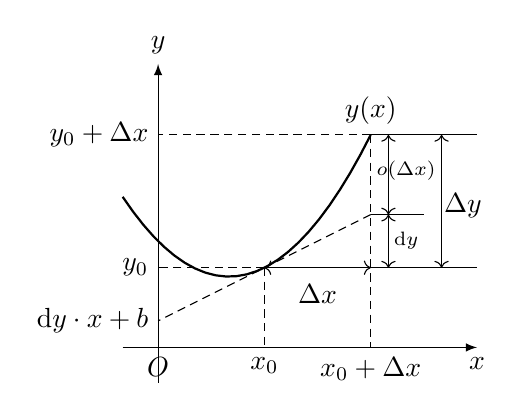
\begin{tikzpicture}[scale=0.9]
                \draw[-latex](-0.5,0) -- (4.5,0) node[below]{$x$};
                \draw[-latex](0,-0.5) -- (0,4) node[above]{$y$};
                \draw[black, thick, domain=-0.5:3] plot (\x,{pow(\x-1,2)/2+1}) node[above]{$y(x)$};
                \filldraw[black] (0,0) node[below]{$O$};
                \draw[black, densely dashed](1.5,1.125) -- (1.5,0) node[below]{$x_0$};
                \draw[black, densely dashed](1.5,1.125) -- (0,1.125) node[left]{$y_0$};
                \draw[black, densely dashed](3,3) -- (3,0) node[below]{$x_0+\Delta x$};
                \draw[black, densely dashed](3,3) -- (0,3) node[left]{$y_0+\Delta x$};
                \draw[black, densely dashed](3,1.875) -- (0,0.375) node[left]{$\textrm{d}y\cdot x+b$};
                \draw[<->, black](1.5,1.125) -- (3,1.125);
                \draw[<->, black](4,1.125) -- (4,3);
                \draw[<->, black](3.25,1.125) -- (3.25,1.875);
                \draw[<->, black](3.25,3) -- (3.25,1.875);
                \draw[black](3,3) -- (4.5,3);
                \draw[black](3,1.125) -- (4.5,1.125);
                \draw[black](3,1.875) -- (3.75,1.875);
                \filldraw[black] (2.25,0.75) node{$\Delta x$};
                \filldraw[black] (4.3,2) node{$\Delta y$};
                \filldraw[black] (3.5,1.5) node{\scriptsize{$\textrm{d}y$}};
                \filldraw[black] (3.5,2.5) node{\scriptsize{$o(\Delta x)$}};
            \end{tikzpicture}
        \end{minipage} \medskip

        所以可微就是用简单线性取代复杂线性,如图用直线取替代曲线。微分就是瞬时改变量,而导数就是瞬时改变速率。

        \subsection{基本运算}

        \subsubsection{四则运算}

        若函数可导:

        \begin{enumerate}
            \item 和差的微分:$\textrm{d}[ku(x)\pm lv(x)]=k\textrm{d}u(x)\pm l\textrm{d}v(x)$。
            \item 积的微分:$\textrm{d}[u(x)v(x)]=u(x)\textrm{d}v(x)+v(x)\textrm{d}u(x)$。
            \item 商的微分:$\textrm{d}\left[\dfrac{u(x)}{v(x)}\right]=\dfrac{v(x)\textrm{d}u(x)-u(x)\textrm{d}v(x)}{[v(x)]^2}$,$v(x)\neq 0$。
            \item 复合函数的微分:链式求导法则$\dfrac{\textrm{d}u}{\textrm{d}x}=\dfrac{\textrm{d}u}{\textrm{d}y}\cdot\dfrac{\textrm{d}y}{\textrm{d}x}$。
        \end{enumerate}

        \subsubsection{微分形式不变性}

        \textcolor{violet}{\textbf{定义:}}设$y=f(u)$可微,$u=g(x)$可微,则$y=f(g(x))$可微,且$\textrm{d}y=y'_{x}\textrm{d}x=y'_{u}\textrm{d}u$。即对哪个变量求导都是一样的,即$\textrm{d}\{f\,[g(x)]\}=f\,'[g(x)]g'(x)\textrm{d}x$。

        一阶微分形式不变性指:$\textrm{d}f\,(\varsigma)=f\,'(\varsigma)\textrm{d}\varsigma$,无论$\varsigma$是什么(类似导数的链式求导法则)。

        \textbf{例题:}设$y=e^{\sin(\ln x)}$,求$\textrm{d}y$。

        解:$\because y=e^{\sin(\ln x)} \therefore$

        $
        \begin{aligned}
            \textrm{d}y &=\textrm{d}e^{\sin(\ln x)} \\
            & =e^{\sin(\ln x)}\cdot\textrm{d}(\sin(\ln x)) \\
            & =e^{\sin(\ln x)}\cdot\cos(\ln x)\cdot\textrm{d}\ln x \\
            & =e^{\sin(\ln x)}\cdot\cos(\ln x)\cdot\dfrac{1}{x}\textrm{d}x
        \end{aligned}
        $

        \section{基本求导公式}

        \subsection{对幂指函数}

        \begin{center}
            \begin{tabular}{|c|c|c|c|}
                \hline
                原函数 & 导函数 & 原函数 & 导函数\\ \hline
                $C$ & $0$ & $n^x$ & $n^x\ln n$ \\ \hline
                $\log_ax$ & $\dfrac{1}{x\ln a}$ & $\ln x=\ln\vert x\vert$ & $\dfrac{1}{x}$ \\ \hline
                $x^n$ & $nx^{n-1}$ & $\sqrt[n]{x}$ & $\dfrac{x^{-\frac{n-1}{n}}}{n}$ \\ \hline
                $\dfrac{1}{x^n}$ & $-\dfrac{n}{x^{n+1}}$ & & \\
                \hline
            \end{tabular}
        \end{center}

        \subsection{三角与反三角函数}

        \begin{center}
            \begin{tabular}{|c|c|c|c|}
                \hline
                原函数 & 导函数 & 原函数 & 导函数\\ \hline
                $\sin x$ & $\cos x$ & $\cos x$ & $-\sin x$ \\ \hline
                $\tan x$ & $\dfrac{1}{\cos^2x}=\sec^2x$ & $\cot x$ & $\dfrac{1}{\sin^2x}=\csc^2x$ \\ \hline
                $\sec x$ & $\sec x\tan x$ & $\csc x$ & $-\csc x\cot x$ \\ \hline
                $\arcsin x$ & $\dfrac{1}{\sqrt{1-x^2}}$ & $\arccos x$ & $-\dfrac{1}{\sqrt{1-x^2}}$ \\ \hline
                $\arctan x$ & $\dfrac{1}{1+x^2}$ & $\textrm{arccot}\,x$ & $-\dfrac{1}{1+x^2}$ \\ \hline
                $\textrm{arcsec}\,x$ & $\dfrac{1}{x\sqrt{x^2-1}}$ & $\textrm{arccsc}\,x$ & $-\dfrac{1}{x\sqrt{x^2-1}}$ \\
                \hline
            \end{tabular}
        \end{center}

        \subsection{双曲与反双曲函数}

        \begin{itemize}
            \item 双曲正弦:$\textrm{sinh}\,x=\textrm{sh}\,x=\dfrac{e^{x}-e^{-x}}{2}$。
            \item 双曲余弦:$\textrm{cosh}\,x=\textrm{ch}\,x=\dfrac{e^{x}+e^{-x}}{2}$。
            \item 双曲正切:$\textrm{tanh}\,x=\textrm{th}\,x=\dfrac{\textrm{sinh}\,x}{\textrm{cosh}\,x}=\dfrac{e^{x}-e^{-x}}{e^{x}+e^{-x}}$。
            \item 双曲余切:$\textrm{coth}\,x=\dfrac{\textrm{cosh}\,x}{\textrm{sinh}\,x}=\dfrac{e^{x}+e^{-x}}{e^{x}-e^{-x}}$。
            \item 双曲正割:$\textrm{sech}\,x=\dfrac{1}{\textrm{cosh}\,x}=\dfrac{2}{e^{x}+e^{-x}}$。
            \item 双曲余割:$\textrm{csch}\,x=\dfrac{1}{\textrm{sinh}\,x}=\dfrac{2}{e^{x}-e^{-x}}$。
            \item 反双曲正弦:$\textrm{arcsinh}\,x=\ln\left(x+\sqrt{x^2+1}\right)$。
            \item 反双曲余弦:$\textrm{arccosh}\,x=\ln\left(x+\sqrt{x^2-1}\right)$。
            \item 反双曲正切:$\textrm{arctanh}\,x=\dfrac{1}{2}\ln\left(\dfrac{1+x}{1-x}\right)$。
        \end{itemize}

        \begin{center}
            \begin{tabular}{|c|c|c|c|}
                \hline
                原函数 & 导函数 & 原函数 & 导函数\\ \hline
                $\textrm{sinh}\,x$ & $\textrm{cosh}\,x$ & $\textrm{cosh}\,x$ & $\textrm{sinh}\,x$ \\ \hline
                $\textrm{tanh}\,x$ & $\dfrac{1}{\textrm{cosh}\,x^2}$ & $\textrm{arcsinh}\,x$ & $\dfrac{1}{\sqrt{x^2+1}}$ \\ \hline
                $\textrm{arccosh}\,x$ & $\dfrac{1}{\sqrt{x^2-1}}$ & $\textrm{arctan}\,x$ & $\dfrac{1}{1-x^2}$ \\
                \hline
            \end{tabular}
        \end{center}

        \section{函数中值定理}

        都假定$f(x)$在$[a,b]$上连续。

        \subsection{有界与最值定理}

        {\textbf{定理:}}$m\leqslant f(x)\leqslant M$,其中$m$,$M$分别为$f(x)$在$[a,b]$上的最大值和最小值。

        \subsection{介值定理}

        {\textbf{定理:}}当$m\leqslant\mu\leqslant M$,存在$\xi\in[a,b]$,使得$f(\xi)=\mu$。

        \subsection{平均值定理}

        {\textbf{定理:}}当$a<x_1<x_2<\cdots<x_n<b$时,在$[x_1,x_n]$内至少存在一点$\xi$,使得$f(\xi)=\dfrac{f(x_1)+f(x_2)+\cdots+f(x_n)}{n}$。

        证明:已知$f(x)$在$[x_1,x_n]$上连续,根据有界与最值定理,$m\leqslant f(x)\leqslant M$。

        即$m\leqslant f(x_1)\leqslant M$、$m\leqslant f(x_2)\leqslant M$……$m\leqslant f(x_n)\leqslant M$。

        将这些式子全部相加,得到$nm\leqslant f(x_1)+f(x_2)+\cdots+f(x_n)\leqslant nM$。

        所以$m\leqslant\dfrac{f(x_1)+f(x_2)+\cdots+f(x_n)}{n}\leqslant m$。

        由介值定理,可知存在$\xi\in[a,b]$使得$f(\xi)=\dfrac{f(x_1)+f(x_2)+\cdots+f(x_n)}{n}$。

        \subsection{零点定理}

        {\textbf{定理:}}当$f(a)\cdot f(b)<0$时,存在$\xi\in(a,b)$,使得$f(\xi)=0$。

        \section{微分中值定理}

        四个定理都是建立局部与整体的关系,利用导数控制函数,反之不能使用函数控制导数。

        $\text{罗尔定理}\xrightleftharpoons[\text{特例:}f(a)=f(b)]{\text{泛化:任意端点值}}\text{拉格朗日中值定理}\xrightleftharpoons[\text{特例:}F(x)=x]{\text{泛化:参数方程}}\text{柯西中值定理}$

        \subsection{罗尔定理}

        \subsubsection{定义}

        极值\textcolor{violet}{\textbf{定义:}}若$\exists\delta>0$,使$\forall x\in U(x_0,\delta)$恒有$f(x)\geqslant f(x_0)$,则$f(x)$在$x_0$处取极小值,恒有$f(x)\leqslant f(x_0)$,则$f(x)$在$x_0$处取极大值。

        费马引理\textcolor{violet}{\textbf{定义:}}若$f(x)$在$x_0$处取得极值,且$f(x)$在$x_0$处可导,则$f'(x_0)=0$。

        罗尔定理\textcolor{violet}{\textbf{定义:}}

        \begin{minipage}{0.45\linewidth}
            \begin{enumerate}
                \item $f(x)$在$[a,b]$上连续。
                \item $f(x)$在$(a,b)$内可导。
                \item $f(a)=f(b)$。
            \end{enumerate}

            则$\exists\,\xi\in(a,b)$,使得$f'(\xi)=0$。
        \end{minipage}
        \hfill
        \begin{minipage}{0.45\linewidth}
            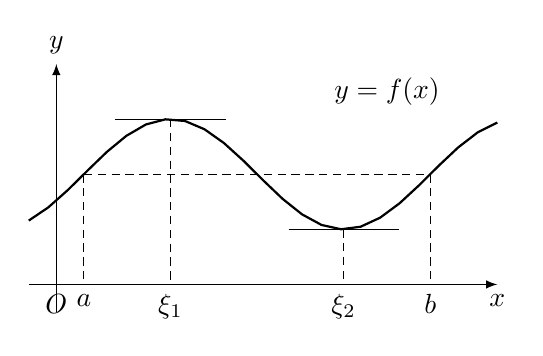
\begin{tikzpicture}[scale=0.7]
                \draw[-latex](-0.5,0) -- (8,0) node[below]{$x$};
                \draw[-latex](0,-0.5) -- (0, 4) node[above]{$y$};
                \filldraw[black] (0,0) node[below]{$O$};
                \draw[black, thick,domain=-0.5:8] plot (\x, {sin((\x-0.5) r)+2});
                \filldraw[black] (6,3.5) node {$y=f(x)$};
                \draw[densely dashed](0.5,2) -- (0.5+2*pi, 2);
                \draw[densely dashed](0.5,2) -- (0.5, 0) node[below]{$a$};
                \draw[densely dashed](0.5+2*pi,2) -- (0.5+2*pi, 0) node[below]{$b$};
                \draw[densely dashed](0.5+pi/2,3) -- (0.5+pi/2, 0) node[below]{$\xi_1$};
                \draw[densely dashed](0.5+pi/2*3,1) -- (0.5+pi/2*3, 0) node[below]{$\xi_2$};
                \draw[black](pi/2-0.5,3) -- (1.5+pi/2,3);
                \draw[black](pi/2*3-0.5,1) -- (1.5+pi/2*3,1);
            \end{tikzpicture}
        \end{minipage}

        \subsubsection{推广}

        \begin{itemize}
            \item 设$f(x)$在$(a,b)$内可导,$\lim\limits_{x\to a^+}f(x)=\lim\limits_{x\to b^-}f(x)=A$,则在$(a,b)$内至少存在一点$\xi$,使得$f'(\xi)=0$。
            \item 设$f(x)$在$(a,b)$内可导,$\lim\limits_{x\to a^+}f(x)=\lim\limits_{x\to b^-}f(x)=\pm\infty$,则在$(a,b)$内至少存在一点$\xi$,使得$f'(\xi)=0$。
            \item 设$f(x)$在$(a,+\infty)$内可导,$\lim\limits_{x\to a^+}f(x)=\lim\limits_{x\to+\infty}f(x)=A$,则在$(a,+\infty)$内至少存在一点$\xi$,使得$f'(\xi)=0$。
            \item 设$f(x)$在$(\infty,+\infty)$内可导,$\lim\limits_{x\to-\infty}f(x)=\lim\limits_{x\to+\infty}f(x)=A$,则在$(-\infty,+\infty)$内至少存在一点$\xi$,使得$f'(\xi)=0$。
        \end{itemize}

        \subsection{拉格朗日中值定理}

        \begin{enumerate}
            \item $f(x)$在$[a,b]$上连续。
            \item $f(x)$在$(a,b)$内可导。
        \end{enumerate}

        则$\exists\,\xi\in(a,b)$,使得$f(b)-f(a)=f'(\xi)(b-a)$。

        拉格朗日中值定理的几何意义:若连续曲线$y=f(x)$的弧$\wideparen{AB}$上除端点外处处具有不垂直于$x$轴的切线,则这弧上至少有一点$C$使曲线在该点处的切线平行于弦$AB$。

        其中$f(b)-f(a)=f'[a+\theta(b-a)](b-a)(0<\theta<1)$,$\because f'(\xi)=f'[a+(\xi-a)]=f'[a+\dfrac{\xi-a}{b-a}(b-a)]$。\medskip

        有限增量公式\textcolor{violet}{\textbf{定义:}}$\Delta y=f(x_0+\Delta x)-f(x_0)=f'[x_0+\theta\Delta x]\Delta x(0<\theta<1)$。

        有限增量公式中的$\Delta x$不一定很小,这个是一个增量的准确公式。即将增量$\Delta y$用$\Delta x$和该线段上某点的导数来表示,与微分值不同的是这个是个准确值而不是近似值,但是不好用,因为$\theta$未知。

        推论:$f(x)$在$I$上连续且可导,则$I$上$f(x)=C\Leftrightarrow f'(x)\equiv 0$。

        \textbf{例题:}证明$x>0$时,$\dfrac{x}{1+x}<\ln(1+x)<x$。

        证明:令$f(x)=\ln x$,又$\ln 1=0$,$\therefore\ln(1+x)=\ln(1+x)-\ln 1$。

        根据拉格朗日中值定理$\ln(1+x)-\ln 1=f'(\xi)x=\dfrac{x}{\xi}(1<\xi<1+x)$。

        又$\dfrac{x}{1+x}<\dfrac{x}{\xi}<x$,$\therefore$得证。

        \subsection{柯西中值定理}

        \begin{enumerate}
            \item $f(x)$与$F(x)$在$[a,b]$上连续。
            \item $f(x)$与$F(x)$在$(a,b)$内可导,且$\forall x\in(a,b)$,$F'(x)\neq 0$。
        \end{enumerate}

        则$\exists\,\xi\in(a,b)$,使得$\dfrac{f(b)-f(a)}{F(b)-F(a)}=\dfrac{f'(\xi)}{F'(\xi)}$。

        \subsection{泰勒中值定理}

        即携带拉格朗日余项的泰勒公式。

        设$f(x)$在区间$I$上$(n+1)$阶可导,$x_0\in I$,那么对$\forall x\in I$,$\exists\xi$使得$f(x)=f(x_0)+f'(x_0)(x-x_0)+\cdots+\dfrac{f^{(n)}(x_0)}{n!}(x-x_0)^n+R_n(x)$。

        拉格朗日型余项:$R_n(x)=\dfrac{f^{(n+1)(\xi)}}{(n+1)!}(x-x_0)^{n+1}$,$\xi\in I$。用于证明。

        陪亚诺型余项:$R_n(x)=o((x-x_0)^n)$。用于求极限,因为余项太粗糙。

        \section{洛必达法则}

        \subsection{定理}

        若当$x\to a$或$x\to\infty$时两个函数$f(x)F(x)$都趋向0或无穷大,那么极限$\lim\limits_{x\to \frac{a}{\infty}}\dfrac{f(x)}{F(x)}$可能存在,也可能不存在,这种极限就是不定式。\medskip

        \textcolor{aqua}{\textbf{定理:}}

        \begin{enumerate}
            \item 当$x\to a\text{或}\infty$时,函数$f(x)$,$g(x)$都趋向0或无穷大。
            \item $f'(x)$和$F'(x)$在点$a$的某去心邻域内,或$\vert x\vert$大于充分大的正数时,存在,且$g'(x)\neq 0$。
            \item $\lim\limits_{x\to a}\dfrac{f'(x)}{g'(x)}$或$\lim\limits_{x\to\infty}\dfrac{f'(x)}{g'(x)}$存在或无穷大。
            \item $\lim\limits_{x\to a}\dfrac{f(x)}{g(x)}=\lim\limits_{x\to a}\dfrac{f'(x)}{g'(x)}$或$\lim\limits_{x\to\infty}\dfrac{f(x)}{g(x)}=\lim\limits_{x\to\infty}\dfrac{f'(x)}{g'(x)}$。
        \end{enumerate}

        \subsection{注意事项}

        \begin{enumerate}
            \item 如果函数比值不为$\dfrac{0}{0}$或$\dfrac{\infty}{\infty}$型,则不能使用洛必达法则。
            \item 若求导后极限仍为$\dfrac{0}{0}$或$\dfrac{\infty}{\infty}$型,则可以继续使用洛必达法则。
            \item 若$\lim\limits_{x\to a}\dfrac{f'(x)}{g'(x)}$不存在且不为$\infty$,不能反推$\lim\limits_{x\to a}\dfrac{f(x)}{g(x)}$不存在也不为$\infty$,这时候洛必达法则是失效的。
            \item 洛必达法则除了可以解决$\dfrac{0}{0}$型、$\dfrac{\infty}{\infty}$型,还可以将$0\cdot\infty$、$\infty-\infty$、$1^\infty$、$\infty^0$、$0^0$类型进行变型来使用洛必达。
        \end{enumerate}

        对于第三个注意点:$\lim\limits_{x\to 0}\dfrac{x^2\cdot\sin\dfrac{1}{x}}{x}=\lim\limits_{x\to 0}x\cdot\sin\dfrac{1}{x}=0$。

        而使用洛必达法则:\medskip

        $\lim\limits_{x\to 0}\dfrac{x^2\cdot\sin\dfrac{1}{x}}{x}=\lim\limits_{x\to 0}\left(2x\cdot\sin\dfrac{1}{x}-\cos\dfrac{1}{x}\right)=\lim\limits_{x\to 0}\left(-\cos\dfrac{1}{x}\right)=\text{不存在}$

        \section{泰勒公式}

        非常重要。过去的很多定义如等价无穷小都是基于泰勒公式。

        \subsection{定义}

        是一个用函数在某点的信息描述其附近取值的公式。如果函数满足一定的条件,泰勒公式可以用函数在某一点的各阶导数值做系数构建一个多项式来近似表达这个函数。即形式:$f(x)=\sum ax^n$。

        简单来说,泰勒公式就是一个近似表达函数的公式。其增量趋向0。

        对于泰勒公式以及之前的中值定理等相关延申见\href{https://www.zhihu.com/question/25627482}{知乎回答}。

        \subsection{泰勒定理}

        拉格朗日定理是泰勒定理的特例。泰勒定理也称为泰勒中值定理,与之前的三大中值定理组成四大中值定理,前面的三大中值定理建立函数与一阶导数的关系,而泰勒定理建立函数与高阶导数之间的关系。

        \subsubsection{皮亚诺余项}

        设$f(x)$在$x_0$处$n$阶可微,则$f(x)=\sum\limits_{k=0}^n\dfrac{f^{(k)}(x_0)}{k!}(x-x_0)^k+o((x-x_0)^n)$。这个就是带皮亚诺余项的泰勒公式。\medskip

        $f(x)=\sum\limits_{k=0}^n\dfrac{f^{(k)}(x_0)}{k!}(x-x_0)^k$就是$f(x)$在$x_0$处的$n$次泰勒多项式,$o((x-x_0)^n)$就是函数的皮亚诺余项。

        缺点:

        \begin{enumerate}
            \item 只给出余项的定性描述,不能进行定量分析。
            \item 适用范围小。
        \end{enumerate}

        \subsubsection{拉格朗日余项}

        设$f(x)$在$x_0$处$n+1$阶可微,$x_0\in I$则$\forall x\in I$,$\exists\,\xi\in I(\xi\in(x_0,x))$使得$f(x)=\sum\limits_{k=0}^n\dfrac{f^{(k)}(x_0)}{k!}(x-x_0)^k+\dfrac{f^{(n+1)}(\xi)}{(n+1)!}(x-x_0)^{n+1}$。这个就是带拉格朗日余项的泰勒公式。

        $R_n(x)=\dfrac{f^{(n+1)}(\xi)}{(n+1)!}(x-x_0)^{n+1}$就是函数的拉格朗日余项。

        根据拉格朗日中值定理推广的方式:$R_n(x)=\dfrac{f^{(n+1)}[x_0+\theta(x-x_0)]}{(n+1)!}(x-x_0)^{n+1}(\theta\in(0,1))$。

        若$\vert f^{(n+1)}(x)\vert\leqslant M$,则$\vert R_n(x)\vert=\dfrac{\vert f^{(n+1)}(\xi)\vert}{(n+1)!}\vert x-x_0\vert^{n+1}\leqslant\dfrac{M}{(n+1)!}\vert x-x_0\vert^{n-1}$。

        特点:

        \begin{enumerate}
            \item 进行定量研究。
            \item 可以进行整体的研究。
            \item 计算量较大。
        \end{enumerate}

        \subsection{泰勒展开}

        \subsubsection{麦克劳林公式}

        当$x_0=0$时$f(x)=f(0)+f'(0)x+\dfrac{f''(0)}{2!}x^2+\cdots+\dfrac{f^{(n)(0)}}{n!}x^n+\text{余项}$为麦克劳林公式:

        \begin{enumerate}
            \item $\sin x=x-\dfrac{x^3}{3!}+o(x^3)=\sum\limits_{k=0}^n(-1)^{n-1}\dfrac{x^{2n-1}}{(2n-1)!}$。
            \item $\cos x=1-\dfrac{x^2}{2!}+\dfrac{x^4}{4!}+o(x^4)=\sum\limits_{k=0}^n(-1)^n\dfrac{x^{2n}}{(2n)!}$。
            \item $\arcsin x=x+\dfrac{x^3}{3!}+o(x^3)=\sum\limits_{k=0}^n\dfrac{x^{2n-1}}{(2n-1)!}$。
            \item $\tan x=x+\dfrac{x^3}{3}+o(x^3)$。
            \item $\arctan x=x-\dfrac{x^3}{3}+o(x^3)$。
            \item $\ln(1+x)=x-\dfrac{x^2}{2}+\dfrac{x^3}{3}+o(x^3)=\sum\limits_{k=0}^n(-1)^n\dfrac{x^n}{n}$。
            \item $e^x=1+x+\dfrac{x^2}{2!}+\dfrac{x^3}{3!}+o(x^3)=\sum\limits_{k=0}^n\dfrac{x^n}{n!}$。
            \item $(1+x)^\alpha=1+\alpha\cdot x+\dfrac{\alpha\cdot(\alpha-1)}{2!}x^2+o(x^2)$。
        \end{enumerate}

        其中$o(x^\alpha)$为佩亚诺余项,其非常小。

        同样可以对泰勒展开式进行变形:$x-\sin x\sim\dfrac{x^3}{6}$,$x+\sin x\sim 2x$。

        如:

        $\lim\limits_{x\to 0}\dfrac{[\sin x-\sin(\sin x)]\sin x}{x^4}=\dfrac{\dfrac{1}{6}\sin^3x\cdot\sin x}{x^4}=\dfrac{\dfrac{1}{6}\sin^4x}{x^4}=\dfrac{1}{6}$

        \subsubsection{泰勒公式计算}

        先写出$y=f(x)$的泰勒公式或麦克劳林公式,再通过比较系数来获得$f^{(n)}(x_0)$:

        \begin{enumerate}
            \item 任何一个无穷阶可导的函数(在收敛的情况下)都可以写为: \medskip \\
            $y=f(x)=\sum_{n=0}^\infty\dfrac{f^{(n)}(x_0)}{n!}(x-x_0)^n$ 或 $y=f(x)=\sum_{n=0}^\infty\dfrac{f^{(n)}(0)}{n!}x^n$。
            \item 给出的任意一个具体的无穷阶可导函数$y=f(x)$都可以通过已知的公式展开为幂级数。
            \item 而函数的展开式具有唯一性,比较步骤一步骤二的公式的系数就可以获取倒$f^{(n)}(x_0)$或$f^{(n)}(0)$。
        \end{enumerate}

        \textbf{例题:}设$y=x^3\sin x$,求$y^{(6)}(0)$。\medskip

        解:\ding{172}$y=\sum_{n=0}^\infty\dfrac{y^{(n)}(0)}{n!}x^n$。\medskip

        $\because$需要结果的导数阶数为6,所以最后得到的次数为6就可以了。\medskip

        \ding{173}$\therefore y=x^3\left(x-\dfrac{1}{6}x^3+\cdots\right)=x^4-\dfrac{1}{6}x^6+\cdots$(不要写$o(x^n)$,因为这里$x$并不是趋向0的)。

        \ding{174}步骤一的抽象函数当$n=6$时为$\dfrac{y^{(6)}(0)}{6!}x^6$,它应该与步骤二得到的$x^4-\dfrac{1}{6}x^6+\cdots$的6阶项的系数相等。

        $\therefore \dfrac{y^{(6)}(0)}{6!}=-\dfrac{1}{6}\Rightarrow y^{(6)}(0)=-5!=-120$。

        \subsection{展开幂的选择}

        泰勒公式展开时应该展开到多少次幂?

        \subsubsection{\texorpdfstring{$\dfrac{A}{B}$}\ 型,上下同阶}

        当分母或分子式$x$的$k$次幂那么应该把分母或分子展开到对应的次数幂。\medskip

        如$\lim\limits_{x\to 0}\dfrac{x-\sin x}{x^3}$展开为三次:\medskip

        $\lim\limits_{x\to 0}\dfrac{x-\sin x}{x^3}=\lim\limits_{x\to 0}\dfrac{x-\left[x-\dfrac{1}{6}x^3+o(x^3)\right]}{x^3}=\lim\limits_{x\to 0}\dfrac{\dfrac{1}{6}x^3+o(x^3)}{x^3}=\dfrac{1}{6}$

        \subsubsection{\texorpdfstring{$A-B$}\ 型,幂次最高}

        将$A$,$B$分别展到他们系数不相等的$x$的最高次幂为止。

        如已知当$x\to 0$时,$\cos x-e^{-\frac{x^2}{2}}$与$ax^k$为等价无穷小,求$a$,$b$。

        泰勒展开:

        $\cos x-e^{-\frac{x^2}{2}}= 1-\dfrac{x^2}{2}+\dfrac{1}{24}x^4+o(x^4)-\left(1-\dfrac{x^2}{2}+\dfrac{1}{8}x^4+o(x^4)\right)$

        $=-\dfrac{1}{12}x^4+o(x^4)\sim -\dfrac{1}{12}x^4$

        $\therefore a=-\dfrac{1}{12},b=4$。

        \textbf{例题:}求解$\lim\limits_{x\to 0}\dfrac{\sin^2x-x^2}{e^{x^4}-1}$。

        解:首先由泰勒展开式$e^x=1+x+o(x)$,得到$e^x-1\sim x$。

        $\therefore e^{x^4}-1\sim x^4$。

        然后泰勒展开:

        $x-\sin x=1\cdot x^1+0\cdot x^3 - (1\cdot x^1-\dfrac{1}{6}x^3+o(x^3))= \dfrac{1}{6}x^3+o(x^3)\sim\dfrac{1}{6}x^3$

        $x+\sin x=x-(-\sin x)=1\cdot x^1-(-1\cdot x^1)+o(x)=2x+o(x)\sim 2x$ \medskip

        $\therefore\lim\limits_{x\to 0}\dfrac{\sin^2x-x^2}{e^{x^4}-1}=\lim\limits_{x\to 0}\dfrac{(\sin x+x)(\sin x-x)}{x^4}=\lim\limits_{x\to 0}\dfrac{2x\cdot\left(-\dfrac{1}{6}x^3\right)}{x^4}=-\dfrac{1}{3}$

        \section{函数单调性与曲线凹凸性}

        \subsection{函数单调性}

        \textcolor{aqua}{\textbf{定理:}}

        \begin{enumerate}
            \item 函数$f(x)$在区间$[a,b]$上连续,在$(a,b)$内可导。
            \item 若$(a,b)$内$f'(x)\geqslant 0$,且等号只有有限个点上成立,则$f(x)$在$[a,b]$上单调增加。
            \item 若$(a,b)$内$f'(x)\leqslant 0$,且等号只有有限个点上成立,则$f(x)$在$[a,b]$上单调减少。
        \end{enumerate}

        \textbf{例题:}证明$x>0$时,$x-\dfrac{x^3}{6}<\sin x<x$。

        证明:首先令$f(x)=x-\sin x$,而$f(0)=0$。

        $f'(x)=1-\cos x\geqslant 0$,则$f(x)$在$R$上递增。

        $\therefore$在$(0,+\infty]$上$f(x)>f(0)=0$,即$x>\sin x$。

        令$g(x)=\sin x-x-\dfrac{x^3}{6}$,而$g(0)=0$。

        $g'(x)=\cos x-1+\dfrac{x^2}{2}\geqslant 0$,则$g(x)$在$R$上递增。

        $\therefore$在$(0,+\infty]$上$g(x)>g(0)=0$,即$\sin x>x-\dfrac{x^3}{6}$。

        得证。

        \subsection{曲线凹凸性与拐点}

        \textcolor{violet}{\textbf{定义:}}若函数$f(x)$在区间$I$上连续,且对$I$上任意两点$x_1,x_2$恒有:

        \begin{enumerate}
            \item $f(\dfrac{x_1+x_2}{2})<\dfrac{f(x_1)+f(x_2)}{2}$,则$f(x)$在$I$上凹。
            \item $f(\dfrac{x_1+x_2}{2})>\dfrac{f(x_1)+f(x_2)}{2}$,则$f(x)$在$I$上凸。
        \end{enumerate}

        而当凹凸性发生改变的点就是拐点。

        \textcolor{aqua}{\textbf{定理:}}

        \begin{enumerate}
            \item 函数$f(x)$在区间$[a,b]$上连续,在$(a,b)$内二阶可导。
            \item 若$(a,b)$内$f''(x)>0$,则$f(x)$在$[a,b]$上凹。
            \item 若$(a,b)$内$f''(x)<0$,则$f(x)$在$[a,b]$上凸。
        \end{enumerate}

        拐点的二阶导数等于0,或拐点在二阶导数不存在的点。

        \textbf{例题:}证明凹凸性与二阶导数的关系。

        证明:不妨先证明凹函数与二阶导数的关系。已知$f''(x)>0$

        不妨设$x_1<x_2$,且$\dfrac{x_1+x_2}{2}=x_0$。

        $f(x_1)+f(x_2)-2(x_0)=[f(x_2)-f(x_0)]-[f(x_1)-f(x_0)]$

        $\xRightarrow{\text{拉格朗日中值定理}}=f'(\xi_2)(x_2-x_0)-f'(\xi_1)(x_0-x_1)=\dfrac{x_2-x_1}{2}[f'(\xi_2)-f'(\xi_1)]>0$

        $\therefore f''(x)>0\Rightarrow f(\dfrac{x_1+x_2}{2})<\dfrac{f(x_1)+f(x_2)}{2}$。

        \section{函数极值与最值}

        \subsection{函数极值}

        极值\textcolor{violet}{\textbf{定义:}}若$\exists\,\delta>0$,使

        $\forall x\in U(x_0,\delta)$恒有$f(x)\geqslant f(x_0)$,则$f(x)$在$x_0$取极小值。

        $\forall x\in U(x_0,\delta)$恒有$f(x)\leqslant f(x_0)$,则$f(x)$在$x_0$取极大值。

        \textcolor{aqua}{\textbf{定理:}}(极值必要条件)

        若$f(x)$在$x_0$处可导,且$x_0$处取得极值,则$f'(x_0)=0$。

        \textcolor{aqua}{\textbf{定理:}}(极值第一充分条件)

        若$f(x)$在$\mathring{U}(x_0,\delta)$内可导,且$f'(x_0)=0$或在$x_0$连续。

        \begin{enumerate}
            \item 若$x<x_0$时,$f'(x)\geqslant 0$,$x>x_0$时$f'(x)\leqslant 0$,则$x_0$取得极大值。
            \item 若$x>x_0$时,$f'(x)\geqslant 0$,$x<x_0$时$f'(x)\leqslant 0$,则$x_0$取得极小值。
            \item 若$f'(x)$在$x_0$处不变号,则无极值点。
        \end{enumerate}

        \textcolor{aqua}{\textbf{定理:}}(极值第二充分条件)

        若$f'(x_0)=0$而且$f''(x_0)\neq 0$:

        \begin{enumerate}
            \item 当$f''(x_0)<0$,则$f(x)$在$x_0$取极大值。
            \item 当$f''(x_0)>0$,则$f(x)$在$x_0$取极小值。
        \end{enumerate}

        \textcolor{aqua}{\textbf{定理:}}(极值第三充分条件)

        若$f(x)$在$x_0$处$n(n\geqslant2)$阶可导,且$f'(x_0)=f''(x_0)=\cdots=f^{(n-1)}(x_0)=0$,$f^{(n)}(x_0)\neq0$,则:

        \begin{enumerate}
            \item 当$n$为偶数时$f(x)$在$x_0$取得极值。当$f^{(n)}(x_0)<0$,则$f(x)$在$x_0$取极大值,当$f^{(n)}(x_0)>0$,则$f(x)$在$x_0$取极小值。
            \item 当$n$为奇数时$f(x)$在$x_0$处无极值。
        \end{enumerate}

        \subsection{函数最值}

        \subsubsection{连续函数闭区间最值}

        \begin{enumerate}
            \item 求出$f(x)$在$(a,b)$内的驻点和不可导的点$x_1,x_2\cdots,x_n$。
            \item 求出函数值$f(x_1),f(x_2)\cdots,f(x_n)$与端点值$f(a),f(b)$。
            \item 比较求出最值。
        \end{enumerate}

        \subsubsection{最值应用题}

        \begin{enumerate}
            \item 建立目标函数并确定定义域。
            \item 求出驻点并计算值。
        \end{enumerate}

        \section{函数图像绘制}

        \subsection{基本步骤}

        \begin{enumerate}
            \item 确定函数定义域,并考察其奇偶性与周期性。
            \item 求出一阶导数与二阶导数,并计算导数为0与不存在的点。
            \item 根据导数判断增减性与凹凸性,并求出极值与拐点。
            \item 求出渐近线。
            \item 确定另外的特殊点。
        \end{enumerate}

        \subsection{函数渐近线}

        \begin{itemize}
            \item 若$\lim\limits_{x\to\infty}f(x)=A$,那么$y=A$就是水平渐近线。
            \item 若$\lim\limits_{x\to x_0}f(x)=\infty$,那么$x=x_0$就是垂直渐近线。
            \item 若$\lim\limits_{x\to\infty}\dfrac{f(x)}{x}=a,b=\lim\limits_{x\to\infty}(f(x)-ax)$,那么$y=ax+b$就是斜渐近线。
        \end{itemize}

        考的比较多的是斜渐进性,计算较复杂,如果能写成$y=f(x)=ax+b+o(x)$,$o(x)$为$x\to\infty$的高阶无穷小,则能快速得到斜渐进线。

        \section{弧微分与曲率}

        \subsection{弧微分}

        \begin{minipage}{0.5\linewidth}
            \begin{tikzpicture}[scale=3]
                \draw[-latex](-0.1,0) -- (1.25,0) node[below]{$x$};
                \draw[-latex](0,-0.1) -- (0,1.25) node[above]{$y$};
                \filldraw[black] (0,0) node[below]{$O$};
                \draw[black, thick,domain=0.4:1.1] plot (\x, \x*\x);
                \filldraw[black] (0.5,1) node {$y=f(x)$};
                \draw[densely dashed](0.5,0.25) -- (0.5, 0) node[below]{$x$};
                \draw[densely dashed](1,1) -- (1, 0) node[below]{$x+\Delta x$};
                \draw[densely dashed](0.5,0.25) -- (1,0.25);
                \filldraw[black](0.5,0.35) node{$y$};
                \filldraw[black](0.95,1.1) node{$y_0$};
                \filldraw[black](0.75,0.35) node{$\Delta x$};
                \filldraw[black](1.1,0.6) node{$\Delta y$};
            \end{tikzpicture}
        \end{minipage}
        \hfill
        \begin{minipage}{0.4\linewidth}
            $\vert\wideparen{yy_0}\vert=S(x)$

            $\Delta y=f(x+\Delta x)-f(x)$

            $(\Delta s)^2\approx(\Delta x)^2+(\Delta y)^2$
        \end{minipage}\medskip

        当偏移量无穷小时,$y=f(x)$所构成的线段就是一条直线,所以:

        \begin{minipage}{0.5\linewidth}
            \begin{tikzpicture}[scale=3]
                \draw[-latex](-0.1,0) -- (1.25,0) node[below]{$x$};
                \draw[-latex](0,-0.1) -- (0,1.25) node[above]{$y$};
                \filldraw[black] (0,0) node[below]{$O$};
                \draw[black, thick,domain=0.4:1.1] plot (\x, \x);
                \filldraw[black] (0.5,1) node {$y=f(x)$};
                \draw[densely dashed](0.5,0.5) -- (0.5, 0) node[below]{$x$};
                \draw[densely dashed](1,1) -- (1, 0) node[below]{$x+\textrm{d}x$};
                \draw[densely dashed](0.5,0.5) -- (1,0.5);
                \filldraw[black](0.5,0.6) node{$y$};
                \filldraw[black](0.95,1.1) node{$y_0$};
                \filldraw[black](0.75,0.35) node{$\textrm{d}x$};
                \filldraw[black](1.1,0.6) node{$\textrm{d}y$};
            \end{tikzpicture}
        \end{minipage}
        \hfill
        \begin{minipage}{0.4\linewidth}
            $\textrm{d}y=f\,(x+\textrm{d}x)-f\,(x)$

            $(\textrm{d}s)^2=(\textrm{d}x)^2+(\textrm{d}y)^2$

            $\textrm{d}s=\sqrt{(\textrm{d}x)^2+(\textrm{d}y)^2}$(弧微分)
        \end{minipage}

        对于弧微分:

        \begin{itemize}
            \item 若直角坐标系下$y=f(x)$,$\textrm{d}s=\sqrt{1+\left(\dfrac{\textrm{d}y}{\textrm{d}x}\right)^2}\textrm{d}x=\sqrt{1+f'^2(x)}\textrm{d}x$,即$\textrm{d}s=\sqrt{1+f'^2(x)}\textrm{d}x$。
            \item 若参数方程下:$x=\phi(t),y=\psi(t)$,$\textrm{d}s=\sqrt{\left(\dfrac{\textrm{d}x}{\textrm{d}t}\right)^2+\left(\dfrac{\textrm{d}y}{\textrm{d}t}\right)^2}\textrm{d}t$\medskip\\$=\sqrt{\psi'^2(t)+\phi'^2(t)}\textrm{d}t$,即$\textrm{d}s=\sqrt{\psi'^2(t)+\phi'^2(t)}\textrm{d}t$。
        \end{itemize}

        \subsection{曲率}

        曲率\textcolor{violet}{\textbf{定义:}}表明曲线在某一点的弯曲程度的数值,针对曲线上某个点的切线方向角对弧长的转动率,通过微分来定义,表明曲线偏离直线的程度。曲率越大,表示曲线的弯曲程度越大。

        曲率的倒数就是\textbf{曲率半径}。\medskip

        \begin{minipage}{0.5\linewidth}
            两点切线改变角相同时,弯曲程度与两点之间的弧长度成反比。

            两点之间的弧长度相同时,弯曲程度与两点切线改变角成正比。
        \end{minipage}
        \hfill
        \begin{minipage}{0.2\linewidth}
            \begin{tikzpicture}[scale=0.6]
                \draw[black, thick,domain=-2:2] plot (\x, {\x*\x});
                \filldraw[black] (-1,1) circle (2pt) node[left]{$M_1$};
                \filldraw[black] (1,1) circle (2pt) node[right]{$N_1$};
                \draw[black](2,3) -- (0,-1);
                \draw[black](-2,3) -- (0,-1);
            \end{tikzpicture}
        \end{minipage}
        \hfill
        \begin{minipage}{0.2\linewidth}
            \begin{tikzpicture}[scale=0.6]
                \draw[black, thick,domain=-1.5:1.5] plot (\x, {2*\x*\x});
                \filldraw[black] (-1/2,1/2) circle (2pt) node[left]{$M_2$};
                \filldraw[black] (1/2,1/2) circle (2pt) node[right]{$N_2$};
                \draw[black](2,3.5) -- (0,-1/2);
                \draw[black](-2,3.5) -- (0,-1/2);
            \end{tikzpicture}
        \end{minipage}

        \begin{minipage}{0.3\linewidth}
            \begin{tikzpicture}[scale=3]
                \draw[-latex](-0.1,0) -- (1.25,0) node[below]{$x$};
                \draw[-latex](0,-0.1) -- (0,1.25) node[above]{$y$};
                \filldraw[black] (0,0) node[below]{$O$};
                \draw[black, thick,domain=-0.1:1.1] plot (\x, \x*\x);
                \draw[densely dashed](0.5,0.25) -- (0.5, 0) node[below]{$x$};
                \draw[densely dashed](1,1) -- (1, 0) node[below]{$x+\Delta x$};
                \filldraw[black](0.5,0.35) node{$y$};
                \filldraw[black](0.95,1.1) node{$y_0$};
                \filldraw[black] (1/2,1/4) circle (0.5pt);
                \filldraw[black] (1,1) circle (0.5pt);
                \draw[black](1,3/4) -- (1/4,0);
                \draw[black](0.6,0.2) -- (9/8,5/4);
                \draw[line width=0.1] (0.85,0.7) arc (50:0:0.1);
                \filldraw[black](1,0.8) node{$\Delta\alpha$};
                \filldraw[black](0.5,0.8) node{$\vert\wideparen{yy_0}\vert=\Delta s$};
            \end{tikzpicture}
        \end{minipage}
        \hfill
        \begin{minipage}{0.6\linewidth}
            $y-y_0$平均曲率:$\hat{k}=\dfrac{\vert\Delta\alpha\vert}{\vert\Delta s\vert}$。\medskip

            $y$曲率:$k=\lim\limits_{\Delta x\to 0}\left\lvert\dfrac{\Delta\alpha}{\Delta s}\right\rvert=\left\lvert\dfrac{\textrm{d}\alpha}{\textrm{d}s}\right\rvert$($\alpha$为$y$处切线与$x$轴所成角)。
        \end{minipage}\medskip

        需要对曲率公式进行化简,得到$s$与$\alpha$关于$x$的表示。根据弧微分的定义:$\textrm{d}s=\sqrt{1+f'^2(x)}\textrm{d}x$。

        而对于$\alpha$:$\tan\alpha=y'=f'(x)$。

        两边对$x$求导:$\sec^2\alpha\cdot\dfrac{\textrm{d}\alpha}{\textrm{d}x}=y''=f''(x)$。

        又$\because\sec^2\alpha=1+\tan^2\alpha=1+y'^2$。

        $\therefore\dfrac{\textrm{d}\alpha}{\textrm{d}x}=\dfrac{y''}{1+y'^2}\Rightarrow\textrm{d}\alpha=\dfrac{y''}{1+y\,'^2}\textrm{d}x$。

        $\therefore \textcolor{aqua}{\textbf{定理:}}k=\left\lvert\dfrac{\textrm{d}\alpha}{\textrm{d}s}\right\rvert=\dfrac{\vert y''\vert}{(1+y'^2)^{\frac{3}{2}}}$。

        对于参数方程,$k=\dfrac{\vert y''x'-y'x''\vert}{\left(x'^2+y'^2\right)^{\frac{3}{2}}}$。

        \subsection{曲率半径}

        \begin{minipage}{0.5\linewidth}
            $\odot\,O$为函数$L$在点$X$处的曲率圆,该圆与$L$在$X$处相切,切线为$T$。

            该点的曲率半径为$R$,其中$R=\dfrac{1}{K}$。
        \end{minipage}
        \hfill
        \begin{minipage}{0.4\linewidth}
            \begin{tikzpicture}[scale=2]
                \draw (-1,0) -- (1,0);
                \node (X) at (0,0)[below]{X};
                \node (O) at (0,0.5)[above]{O};
                \draw[densely dashed] (X) -- (O);
                \filldraw[black] (0.75,0.25) node{$L$};
                \draw[decorate,decoration={brace,mirror,raise=2pt}] (X) -- (O);
                \filldraw[black] (0.2,0.25) node{$R$};
                \filldraw[black] (-0.75,0) node{$T$};
                \draw[black, thick,domain=-1:1] plot (\x, \x*\x);
                \draw[black] (0,0.5) circle (0.5);
            \end{tikzpicture}
        \end{minipage}

        \section{不定积分}

        \subsection{定义}

        设$f(x)$定义在区间$I$上,若存在可导函数$F(x)$,使得$F'(x)=f(x)$对于任意$x\in I$都成立,则称$F(x)$为$f(x)$在区间$I$上的一个\textbf{原函数}。

        \textcolor{aqua}{\textbf{定理:}}任意的两个原函数只相差一个常数。

        在区间$I$上,函数$f(x)$带有任意常数项的原函数$F(x)+C$称为$f(x)/f(x)\,\textrm{d}x$在该区间上的不定积分,记为$\int f(x)\,\textrm{d}x$,其中$\int$为\textbf{积分号},$f(x)$为\textbf{被积函数},$f(x)\,\textrm{d}x$为\textbf{被积表达式},$x$为\textbf{积分变量}。

        积分就是导数的逆运算。$\int f(x)\,\textrm{d}x=F(x)+C$,$F'(x)=f(x)$。

        \subsection{性质}

        \subsubsection{计算性质}

        积分运算就可以将原来求导的方式进行逆运算。其中隐函数求导法与参数方程求导法都可以看作复合函数求导法则的变式。

        积分运算具有两个性质:

        \begin{enumerate}
            \item $\int[f(x)+g(x)]\textrm{d}x=\int f(x)\textrm{d}x+\int g(x)\textrm{d}x$,就是分项积分法。
            \item $\int kf(x)\textrm{d}x=k\int f(x)\textrm{d}x$($k\neq 0$)。
        \end{enumerate}

        复合函数的求导法则的逆运算,就是换元积分法。

        函数乘积的求导法则的逆运算,就是分部积分法。

        \subsubsection{存在性性质}

        即一元函数的常义(区间有限,函数有界)可积性。

        \textcolor{aqua}{\textbf{定理:}}连续函数必有原函数。而反之有原函数不一定是连续函数,可能有第二类间断点。

        \textcolor{aqua}{\textbf{定理:}}含有第一类间断点、无穷间断点的函数$f(x)$在包含其间断点的区间内必没有原函数$F(x)$。(可以用导数介值定理反证,一个函数的导数不可能导出不可导的点)

        若原函数含有震荡间断点则可能导出导函数。

        如$F(x)=\left\{\begin{array}{lcl}
                           x^2\sin\dfrac{1}{x}, & & x\neq 0 \\
                           0, & & x=0
        \end{array}\right.$,$f(x)=\left\{\begin{array}{lcl}
                                             2x\sin\dfrac{1}{x}-\cos\dfrac{1}{x}, & & x\neq 0 \\
                                             0, & & x=0
        \end{array}\right.$。

        这个函数$F(x)$是连续函数,而$f(x)$在靠近0时的极限为$\lim\limits_{x\to 0}(2x\sin\dfrac{1}{x}-\cos\dfrac{1}{x})=-\lim\limits_{x\to 0}\cos\dfrac{1}{x}$是一个振荡间断点。

        \subsection{换元积分法}

        \subsubsection{第一类换元法(凑微分法)}

        \textcolor{aqua}{\textbf{定理:}}$\int f(u)\,\textrm{d}u=F(u)+C$,则$\int f[\varphi(x)]\varphi'(x)\,\textrm{d}x=\int f[\varphi(x)]\,\textrm{d}\varphi(x)=F[\varphi(x)]+C$。

        即用一个中间变量如$t$替换一个$x$的复杂表达式从而让式子更简单接近基本积分公式。

        如$\displaystyle{\int\dfrac{x}{\sqrt{1+x^2}}\textrm{d}x=\dfrac{1}{2}\int\dfrac{\textrm{d}(1+x^2)}{\sqrt{1+x^2}}}=\sqrt{1+x^2}+C$。\medskip

        凑微分法适用于式子比较简单的情况,所凑微分的形式必须符合一个简单积分公式的式子,且有一定的式子可以提出来到微分号后面。

        \textbf{例题:}

        解:$\int(1+3x)^{100}\,\textrm{d}x=\dfrac{1}{3}\int(1+3x)^{100}\,\textrm{d}(1+3x)=\dfrac{1}{303}(1+3x)^{101}+C$。

        $\int\cos^2x\,\textrm{d}x=\dfrac{1}{2}\int(1+\cos 2x)\,\textrm{d}x=\dfrac{1}{2}\left(x+\dfrac{1}{2}\sin 2x\right)+C$。

        $\int\cos^3x\,\textrm{d}x=\int\cos^2\,\textrm{d}\sin x=\int(1-\sin^2x)\,\textrm{d}\sin x=\sin x-\dfrac{1}{3}\sin^3x+C$。\medskip

        $\displaystyle{\int\dfrac{\textrm{d}x}{x\sqrt{1+\ln x}}=\int\dfrac{\textrm{d}(1+\ln x)}{\sqrt{1+\ln x}}}=2\sqrt{1+\ln x}+C$。\medskip

        $\displaystyle{\int\dfrac{\textrm{d}x}{\sqrt{x}(1+x)}=2\int\dfrac{\textrm{d}\sqrt{x}}{1+(\sqrt{x})^2}}=2\arctan\sqrt{x}+C$。\medskip

        $\displaystyle{\int\dfrac{\arcsin\sqrt{x}}{\sqrt{x(1-x)}}\,\textrm{d}x=\int\dfrac{\arcsin\sqrt{x}}{1-x}\cdot\dfrac{\textrm{d}x}{\sqrt{x}}=2\int\dfrac{\arcsin\sqrt{x}}{1-(\sqrt{x})^2}\,\textrm{d}\sqrt{x}}$ \medskip

        $=2\int\arcsin\sqrt{x}\,\textrm{d}\arcsin\sqrt{x}=(\arcsin\sqrt{x})^2+C$。\medskip

        $\displaystyle{\int\dfrac{\textrm{d}x}{\sqrt{a^2-x^2}}}=\displaystyle{\int\dfrac{\textrm{d}\left(\dfrac{x}{a}\right)}{\sqrt{1-\left(\dfrac{x}{a}\right)^2}}}=\arcsin\dfrac{x}{a}+C$。

        $\displaystyle{\int\dfrac{\textrm{d}x}{a^2+x^2}}=\displaystyle{\int\dfrac{\textrm{d}\left(\dfrac{x}{a}\right)}{1+\left(\dfrac{x}{a}\right)^2}}=\dfrac{1}{a}\arctan\dfrac{x}{a}+C$。\medskip

        $\displaystyle{\int\dfrac{\textrm{d}x}{x^2-a^2}}=\displaystyle{\int\dfrac{\textrm{d}x}{(x-a)(x+a)}}=\dfrac{1}{2a}\displaystyle{\int\left(\dfrac{1}{x-a}-\dfrac{1}{x+a}\right)\textrm{d}x}$ \medskip

        $=\dfrac{1}{2a}\left(\displaystyle{\int\dfrac{\textrm{d}(x-a)}{x-a}-\int\dfrac{\textrm{d}(x+a)}{x+a}}\right)=\dfrac{1}{2a}\ln\left\vert\dfrac{x-a}{x+a}\right\vert+C$。

        \subsubsection{第二类换元法}

        \textcolor{aqua}{\textbf{定理:}}设$x=\varphi(t)$为单调可导函数,且$\varphi'(t)\neq 0$,$\int f[\varphi(t)\varphi'(t)]\,\textrm{d}t=F(t)+C$,则$\int f(x)\textrm{d}x=\int f[\varphi(t)\varphi'(t)]\,\textrm{d}t=F(t)+C=F[\varphi^{-1}(x)]+C$。

        第二类换元法适用于无法适用第一类换元法的情况,但是最重要的还是对于中间变量的取值,这个中间变量必须要让原式子更能接近公式,且还要注意到变量取值范围。

        第二类换元法相当于第一类换元法的逆运算,不是将复杂的$x$表达式转为简单的一个$t$,而是将一个简单的$x$转换为一个关于$t$的表达式。这是因为简单的$x$无法求出积分结果,必须通过复杂化$x$“中和”一部分式子来进行转化。

        \textcolor{orange}{注意:}$\varphi'(t)\neq 0$是为了保证中间变量函数具有反函数,而严格单调函数必然有反函数,所以只要能证明这个中间变量函数必然严格单调,那么其实$\varphi'(t)$也可以等于0。

        \textbf{例题:}求$\int\sqrt{a^2-x^2}\,\textrm{d}x(a>0)$。

        解:首先看题目,如果使用凑微分法,那必须从式子中提取出一个式子放到微分后面,且提取后的式子满足一个简单的积分公式。

        这个式子一般就只能提取出$x$到平方号外面,但是提取后式子仍不能变为一个简单微分公式,所以说第一种凑微分法就无法使用,就只能使用第二类换元法。

        这个式子是一个平方取开平方的式子,所以取中间变量后最好让这个式子能被开平方。又涉及到一个常数$a$,所以我们很容易就想到是否可以通过三角函数来作为中间变量。

        所以取$x=a\sin t$,从而$\sqrt{a^2-x^2}=a\cos t$。

        并且还要注意到这个$t$的取值范围。

        因为$x=\varphi(t)$是一个单调可导的函数。所以$\sin t$必须取在单调区间上。

        又$\sqrt{a^2-x^2}$要求$-a\leqslant x\leqslant a$,$-a\leqslant a\sin t\leqslant a$,从而$-1\leqslant\sin t\leqslant 1$。

        且$\varphi'(t)\neq 0$,所以$\cos t\neq 0$。

        所以综上三个条件从而得到一个$t$的定义域:$t\in\left[-\dfrac{\pi}{2},0\right)\cup\left(0,\dfrac{\pi}{2}\right]$。

        但是在$\left[-\dfrac{\pi}{2},\dfrac{\pi}{2}\right]$上$\varphi'(t)=a\sin t$是严格单调递增的,单调函数必然存在反函数,所以$\varphi'(t)$可以等于0,从而$t\in\left[-\dfrac{\pi}{2},\dfrac{\pi}{2}\right]$。

        $\int\sqrt{a^2-x^2}\,\textrm{d}x=a\int\cos t\,\textrm{d}a\sin t=a^2\int\cos^2t\textrm{d}t=\dfrac{a^2}{2}\int(1+\cos 2t)\textrm{d}t=\dfrac{a^2}{2}\left(t+\dfrac{1}{2}\sin 2t\right)+C=\dfrac{a^2}{2}\left(\arcsin\dfrac{x}{a}+\dfrac{x}{a}\sqrt{1-\dfrac{x^2}{a^2}}\right)+C$。

        \textbf{例题:}

        解:已知$\tan^2x+1=\sec^2x$。

        $\displaystyle{\int\dfrac{\textrm{d}x}{\sqrt{a^2+x^2}}}(a>0)$。

        令$x=a\tan t$。

        原式$=\displaystyle{\int\dfrac{a\sec^2t}{a\sec t}\,\textrm{d}t=\int\sec t\,\textrm{d}t}=\ln\vert\sec t+\tan t\vert+C=\ln\bigg\vert\sqrt{1+\dfrac{x^2}{a^2}}+\dfrac{x}{a}\bigg\vert+C$。

        $\displaystyle{\int\dfrac{\textrm{d}x}{\sqrt{x^2-a^2}}}(a>0)$。

        令$x=a\sec t$。

        原式$=\displaystyle{\int\dfrac{a\sec t\tan t}{a\tan t}\,\textrm{d}t}=\ln\bigg\vert\sec t+\tan t\bigg\vert+C=\ln\bigg\vert\dfrac{x}{a}+\sqrt{\dfrac{x^2}{a^2}-1}\vert+C$。\medskip

        所以常用的换元积分替换方式:

        \begin{enumerate}
            \item $\sqrt{a^2-x^2}$:$x=a\sin t(a\cos t)$。
            \item $\sqrt{a^2+x^2}$:$x=a\tan t$。
            \item $\sqrt{x^2-a^2}$:$x=a\sec t$。
        \end{enumerate}

        换元法本质是将式子转换为我们已知的积分公式,所以换元积分法只适合于能转换为积分公式的简单式子上,如果式子比较复杂或形式与大部分积分公式不一致,那么也无法换元了。

        \subsection{分部积分法}

        已知$(uv)'=uv'+u'v$,所以$uv'=(uv)'-u'v$,从而$\int uv'\,\textrm{d}x=\int(uv)'\,\textrm{d}x-\int vu'\,\textrm{d}x$,即$\int u\,\textrm{d}v=uv-\int v\,\textrm{d}u$。

        所以分部积分法的公式就是:$\int u\,\textrm{d}v=uv-\int v\,\textrm{d}u$。

        所以分部积分法的适用方式就是所求积分的式子是一个可拆分为两项不同函数的式子,式子的分式中一个式子不好积分,另一个式子好积分,就可以用好积分的式子来积分计算。

        \subsubsection{基本分部积分}

        \textbf{例题:}

        解:$\int xe^x\,\textrm{d}x=\int x\,\textrm{d}e^x=xe^x-\int e^x\textrm{d}x=xe^x-e^x+C$。

        $\int x\sin x\,\textrm{d}x=-\int x\,\textrm{d}\cos x=-[x\cos x-\int\cos x\,\textrm{d}x]=-[x\cos x-\sin x]+C=\sin x-x\cos x+C$。

        $\int x\ln x\,\textrm{d}x=\dfrac{1}{2}\int\ln x\textrm{d}x^2=\dfrac{1}{2}[x^2\ln x-\ln x^2\textrm{d}\ln x]=\dfrac{1}{2}[x^2\ln x-\ln x\textrm{d}x]=\dfrac{1}{2}x^2\ln x-\dfrac{1}{4}x^2+C$。

        $\int x\arctan x\textrm{d}x=\dfrac{1}{2}\int\arctan x\textrm{d}x^2=\dfrac{1}{2}\left[x^2\arctan x-\displaystyle{\int\dfrac{x^2}{1+x^2}\textrm{d}x}\right]=\\ \dfrac{1}{2}[x^2\arctan x-x+\arctan x]+C$。

        \subsubsection{多次分部积分还原}

        当式子中含有$\sin x$,$\cos x$,$e^x$这种积分后变化不大的因式时,可以适用多步分部积分,然后在右边计算的式子中得到左边目标式子一样的因式,然后移到一边就能得到目标式子的表达式。

        \textbf{例题:}\medskip

        解:

        $
        \begin{aligned}
            \int e^x\sin x\,\textrm{d}x & =\int\sin x\,\textrm{d}e^x \\
            & =e^x\sin x-\int e^x\cos x\,\textrm{d}x \\
            & =e^x\sin x-\int\cos x\,\textrm{d}e^x \\
            & =e^x\sin x-\left[e^x\cos x+\int e^x\sin\,\textrm{d}x\right] \\
            2\int e^x\sin x\,\textrm{d}x & =e^x\sin x-e^x\cos x
        \end{aligned}
        $

        $\therefore\int e^x\sin x\,\textrm{d}x=\dfrac{e^x\sin x-e^x\cos}{2}+C$。

        $
        \begin{aligned}
            \int\sec^3x\,\textrm{d}x =&\int\sec x\,\textrm{d}\tan x \\
            & =\sec x\tan x-\int\tan^2x\sec x\,\textrm{d}x \\
            & =\sec x\tan x-\int\sec^3x\textrm{d}x+\int\sec x\textrm{d}x \\
            2\int\sec^3x\,\textrm{d}x =&[\sec x\tan x+\ln\vert\sec x+\tan x\vert]
        \end{aligned}
        $

        $\therefore\int\sec^3x\,\textrm{d}x =\dfrac{\sec x\tan x+\ln\vert\sec x+\tan x\vert}{2}+C$。

        如上所说分部积分的方法就是找到目标式子中两个因式好求的一部分进行积分,其中好求是指$\textrm{d}v$微分后这个结果会简化整个式子。

        其中$e^x$,$\sin x$,$\cos x$这三个因式求微分后无法简化,所以无法对其微分,除非需要多次分部积分还原间接求出;$x^n$微分后会降幂,所以一般可以积分;而$\ln x$,$\arctan x$,$\arcsin x$微分会转换为幂函数相关的式子降低幂次,如果不对其微分则无法消去这三个函数,所以如果出现这三个因式必然优先微分。

        所以常用的分部积分方式:

        \begin{enumerate}
            \item $\int x^ne^x\,\textrm{d}x$、$\int x^n\sin x\,\textrm{d}x$,$\int x^n\cos x\,\textrm{d}x$:对非幂函数的部分,即对$e^x$或三角函数进行分部。
            \item $\int x^n\ln x\,\textrm{d}x$,$\int x^n\arctan x\,\textrm{d}x$,$\int x^n\arcsin x\,\textrm{d}x$:对幂函数的部分,即对$x^n$进行分部。
            \item $\int e^x\sin x\,\textrm{d}x$,$\int e^x\cos x\,\textrm{d}x$:对哪个部分进行分部都可以,而$e^x$进行分部积分时没有正负号的改变,所以对$e^x$进行分部积分,需要多次分部积分还原。
        \end{enumerate}

        \subsection{有理函数的积分}

        两个多项式的商$\dfrac{P(x)}{Q(x)}$被称为有理函数,或有理分式。

        假设该多项式之间没有公因式,当$P(x)$的次数小于$Q(x)$的次数时称为真分式,否则称为假分式。

        假分式可以分解为多项式与真分式之和。

        真分式$\dfrac{P(x)}{Q(x)}$若可以分解为两个或多个多项式的乘积:$\dfrac{P(x)}{Q(x)}=\dfrac{P_1(x)}{Q_1(x)}+\dfrac{P_2(x)}{Q_2(x)}+\cdots$,则称为将真分式化为部分分式之和。其中$P_i$的最高阶应该低于$Q_i$最高阶次数。

        通过这种化简方式,可以在求以商的形式的有利函数的式子的积分时拆分因式,从而简化积分运算。这种简化运算主要体现在分数的积分为对数。

        即将多项式的积分式子转换为$\displaystyle{\int\dfrac{A}{x-a}\textrm{d}x}$和$\displaystyle{\int\dfrac{A}{(x-a)^n}\textrm{d}x}$等形式。

        当然如果多项式是无法拆分为一次的多个式子,那就无法使用有理函数积分的化简方式。

        \textcolor{aqua}{\textbf{定理:}}

        $\dfrac{P}{(A_0x^a+A_1x^{a-1}+\cdots+A_ax^0)\cdots(N_0x^n+N_1x^{n-1}+\cdots+N_nx^0)}$ \medskip

        $=\dfrac{a_0x^{a-1}+a_1x^{a-2}+\cdots+a_{a-1}x^0}{A_0x^a+A_1x^{a-1}+\cdots+A_ax^0}+\cdots+\dfrac{n_0x^{n-1}+n_1x^{n-2}+\cdots+n_{n-1}x^0}{N_0x^n+N_1x^{n-1}+\cdots+N_nx^0}$ \medskip

        如$\dfrac{2x+3}{(x+1)(x+2)(x^2+3x+1)}=\dfrac{A}{x+1}+\dfrac{B}{x+2}+\dfrac{Cx+D}{x^2+3x+1}$ \medskip

        从而$A(x+2)(x^2+3x+1)+B(x+1)(x^2+3x+1)+(Cx+D)(x+1)(x+2)$

        $=A(x^3+5x^2+7x+2)+B(x^3+4x^2+4x+1)+(Cx^3+(3C+D)x^2+(2C+3D)x+2D)$

        $=(A+B+C)x^3+(5A+4B+3C+D)x^2+(7A+4B+2C+3D)x+(2A+B+2D)$

        从而$A+B+C=0$(\ding{172}),$5A+4B+3C+D=0$(\ding{173}),$7A+4B+2C+3D=2$(\ding{174}),$2A+B+2D=3$(\ding{175})。

        \ding{173}-3×\ding{172}=$2A+B+D=0$(\ding{176})

        \ding{175}-\ding{176}=$D=3$。

        从而$5A+4B+3C=-3$(\ding{173}),$7A+4B+2C=-7$(\ding{174}),$2A+B=-3$(\ding{175})。

        \ding{174}-\ding{173}=$2A-C=-4$(\ding{177})。

        \ding{177}+\ding{172}=$3A+B=-4$(\ding{178})。

        \ding{178}-\ding{175}=$A=-1$。

        从而$B+C=1$(\ding{172}),$4B+3C=2$(\ding{173}),$4B+2C=0$(\ding{174}),$B=-1$(\ding{175})。

        从而$C=2$。

        所以$\dfrac{2x}{(x+1)(x+2)(x^2+3x+1)}=-\dfrac{1}{x+1}-\dfrac{1}{x+2}+\dfrac{2x+3}{x^2+3x+1}$。\medskip

        \textcolor{aqua}{\textbf{定理:}}

        $\dfrac{P}{x^n}=\dfrac{A}{x}+\dfrac{B_0x+B_1}{x^2}+\cdots+\dfrac{N_0x^{n-1}+\cdots+N_{n-1}x^0}{x^n}$ \medskip

        如$\dfrac{2x}{(1+x)(x^2+1)^2}=-\dfrac{1}{2}\dfrac{1}{x+1}+\dfrac{1}{2}\dfrac{x-1}{x^2+1}+\dfrac{x+1}{(x^2+1)^2}$。

        \section{定积分}

        不定积分的概念根据导数的代数定义给出,而定积分则由几何的面积运算引出。

        定积分是积分的一种,是函数在一个区间上积分和的极限。已知$f(x)$为速度函数,则$f'(x)$为速度变化率函数,$\textrm{d}f(x)$为瞬时位移,则$\int_{a}^bf(x)\,\textrm{d}x$为位移函数。

        如果说是微分就是微小改变量的计算,那么积分就是累加无穷个微分得到的整个计算。

        \subsection{定义}

        设函数$f(x)$在区间$[a,b]$上连续,将区间分割为$n$个子区间:$[x_0,x_1],(x_1,x_2],$\\$(x_2,x_3],\cdots,(x_{n-1},x_n]$,其中$x_0=a$,$x_n=b$。并可知各区间长度为$\Delta x_1=x_1-x_0\cdots$,在每个子区间$(x_{i-1},x_i]$上任意取一点$\xi_i(i=1,2,\cdots,n)$,做累计和$\sum\limits_{i=1}^nf(\xi_i)\Delta x_i=\lim\limits_{n\to\infty}\sum\limits_{i=1}^nf(a+\dfrac{b-a}{n}i)\dfrac{b-a}{n}=\lim\limits_{n\to\infty}\sum\limits_{i=1}^nf(\dfrac{i}{n})\dfrac{1}{n}=\int_0^1f(x)\,\textrm{d}x$,这个式子被称为积分和。

        设$\lambda=\max{\Delta x_1,\Delta x_2,\cdots,\Delta x_n}$,从而$\lambda$为最大的区间长度,若$\lambda\to 0$时积分和极限$\lim\limits_{\lambda\to 0}\sum\limits_{i=1}^nf(\xi_i)\Delta x_i$存在,则这个极限就是函数在区间$[a,b]$的定积分,记为$\int_a^bf(x)\,\textrm{d}x$,并称函数$f(x)$在区间$[a,b]$上可积。

        其中$a$为积分下限,$b$为积分上限,区间$[a,b]$为积分区间,函数$f(x)$为被积函数,$x$是积分变量,$f(x)\,\textrm{d}x$为被积表达式,$\int$为积分号。\medskip

        通过数列极限可以计算积分:$\displaystyle{\int_a^bf(x)\,\textrm{d}x=\lim\limits_{n\to\infty}\sum\limits_{i=1}^nf\left(a+\dfrac{b-a}{n}\cdot i\right)\dfrac{b-a}{n}}$。

        \subsection{性质}

        \textcolor{aqua}{\textbf{定理:}}定积分由积分上下限与函数关系确定,与积分变量无关。$\int_a^xf(x)\,\textrm{d}x=\int_a^xf(t)\,\textrm{d}t=\varPhi(x)$。

        \subsubsection{计算性质}

        设函数$f(x)$在区间$[a,b]$上连续,则得到定积分基本计算性质:

        \begin{enumerate}
            \item 当$a=b$时,$\int_a^bf(x)\,\textrm{d}x=0$。
            \item 当$a>b$时,$\int_a^bf(x)\,\textrm{d}x=-\int_b^af(x)\,\textrm{d}x$。
            \item $\int_a^bkf(x)\,\textrm{d}x=k\int_a^bf(x)\,\textrm{d}x$。
            \item $\int_a^b[f(x)\pm g(x)]\,\textrm{d}x=\int_a^bf(x)\,\textrm{d}x\pm\int_a^bg(x)\,\textrm{d}x$。
            \item $\int_a^bf(x)\,\textrm{d}x=\int_a^cf(x)\,\textrm{d}x+\int_c^bf(x)\,\textrm{d}x$,若$c$处于函数的可积区间。
            \item 若$[a,b]$上$f(x)\geqslant 0$,则$\int_a^bf(x)\,\textrm{d}x\geqslant 0$。当$f(x)\equiv0$时等号成立。
            \item 若$[a,b]$上$f(x)\leqslant g(x)$,则$\int_a^bf(x)\,\textrm{d}x\leqslant\int_a^bg(x)\,\textrm{d}x$。
            \item $\left\vert\int_a^bf(x)\,\textrm{d}x\right\vert\leqslant\int_a^b\vert f(x)\vert\,\textrm{d}x$。
            \item 已知$f(x)\in[m,M]$在$[a,b]$上成立,则$m(b-a)\leqslant\int_a^bf(x)\,\textrm{d}x\leqslant M(a-b)$。
            \item 估值定理:当$M$,$m$分别为$f(x)$在$[a,b]$上的最大值和最小值,则$m(b-a)\leqslant\int_a^bf(x)\,\textrm{d}x\leqslant M(b-a)$。
            \item 积分中值定理:$\exists\,\xi\in[a,b]$,使得$\int_a^bf(x)\,\textrm{d}x=f(\xi)(b-a)$。
            \item 积分中值定理推广:设$f(x)\in[a,b]$,$\exists\,\xi\in(a,b)$,使得$\int_a^bf(x)\,\textrm{d}x=f(\xi)(b-a)$。
        \end{enumerate}

        证明第八条:已知$-\vert f(x)\vert\leqslant f(x)\leqslant\vert f(x)\vert$。

        即得到$-\int_a^b\vert f(x)\vert\,\textrm{d}x\leqslant\int_a^bf(x)\,\textrm{d}x\leqslant\int_a^b\vert f(x)\vert\,\textrm{d}x$。

        从而得证。

        证明第十一条积分中值定理:

        设函数$f(x)$在区间$[a,b]$上连续,因为闭区间上连续函数必然有最大最小值,所以设最大值为$M$,最小值为$m$,$M\geqslant m$。

        对$m\leqslant f(x)\leqslant M$两边积分得到:$m(b-a)\leqslant\int_a^bf(x)\,\textrm{d}x\leqslant M(b-a)$。

        同时除以$b-a$得到:$m\leqslant\dfrac{1}{b-a}\int_a^bf(x)\,\textrm{d}x\leqslant M$。

        由连续函数的介值定理,必然存在一个$\xi$,使得$f(\xi)=\dfrac{1}{b-a}\int_a^bf(x)\,\textrm{d}x$。

        从而得到$\exists\,\xi\in[a,b]$,使得$\int_a^bf(x)\,\textrm{d}x=f(\xi)(b-a)$。

        也可以使用下面的变限积分来证明:

        因为$f(x)$连续,所以有积分,设$F(x)=\int_a^xf(t)\,\textrm{d}t$。

        对$F(x)$使用拉格朗日中值定理:$F(b)-F(a)=F'(\xi)(b-a)$,即$\int_a^bf(x)\,\textrm{d}x=f(\xi)(b-a)$,其中$\xi\in(a,b)\subset[a,b]$。

        证明第十二条积分中值定理的推广。令$F(x)=\int_a^xf(t)\,\textrm{d}t$,$F'(x)=f(x)$。

        $\int_a^bf(x)\,\textrm{d}x=F(b)-F(a)=F'(\xi)(b-a)=f(\xi)(b-a)$($a<\xi<b$)。

        \subsubsection{存在性性质}

        充分条件:

        \begin{enumerate}
            \item 设函数$f(x)$在区间$[a,b]$上连续,则$f(x)$在该区间上可积。
            \item 设函数$f(x)$在区间$[a,b]$上单调,则$f(x)$在该区间上可积。
            \item 设函数$f(x)$在区间$[a,b]$上有界,且只有有限个间断点,则$f(x)$在该区间上可积。
        \end{enumerate}

        必要条件:可积函数必然有界。

        \subsubsection{定积分与函数性质}

        \begin{enumerate}
            \item 若函数$f(x)$是周期函数且周期为$T$,$\int_a^{a+T}f(x)\,\textrm{d}x=\int_0^Tf(x)\,\textrm{d}x$,\\$\int_\alpha^{\alpha+nT}f(x)\,\textrm{d}x=n\int_0^Tf(x)\,\textrm{d}x$($n\in N$)对于$\forall a$成立。
            \item 若函数$f(x)$是连续的偶函数,则$\int_{-a}^af(x)\,\textrm{d}x=2\int_0^af(x)\,\textrm{d}x$。
            \item 若函数$f(x)$是连续的奇函数,则$\int_{-a}^af(x)\,\textrm{d}x=0$。
            \item 区间再现公式:若函数$f(x)$为连续函数,则$\int_a^bf(x)\,\textrm{d}x=\int_a^bf(a+b-x)\,\textrm{d}x$。
        \end{enumerate}

        证明定理第一条的第一个式子:根据积分区间可拆性:

        $\int_a^{a+T}f(x)\,\textrm{d}x=\int_0^af(x)\,\textrm{d}x+\int_0^Tf(x)\,\textrm{d}x+\int_T^{a+T}f(x)\,\textrm{d}x$

        其中令$x-T=t$,即$x=t+T$,将$t$代入上下限:$\int_T^{a+T}f(x)\,\textrm{d}x=\int_0^af(t+T)\,\textrm{d}(t+T)$,因为$f(x)$是周期函数,周期为$T$,$\therefore=\int_0^af(t)\,\textrm{d}t=\int_0^af(x)\,\textrm{d}x$。

        $\therefore\int_a^{a+T}f(x)\,\textrm{d}x=\int_0^af(x)\,\textrm{d}x+\int_0^Tf(x)\,\textrm{d}x+\int_0^af(x)\,\textrm{d}x=\int_0^Tf(x)\,\textrm{d}x$。

        证明区间再现公式:令$x=a+b-t$。

        这种方法也称为定积分的\textcolor{orange}{区间再现换元法}。

        $\int_a^bf(x)\,\textrm{d}x=\int_b^af(a+b-t)(-\textrm{d}t)=\int_a^bf(a+b-t)\,\textrm{d}t=\int_a^bf(a+b-x)\,\textrm{d}x$。

        如何使用区间再现换元法来进行计算呢?可能$\int_a^bf(x)\,\textrm{d}x$和$\int_a^bf(a+b-x)\,\textrm{d}x$解不出来,但是可能$\int_a^bf(x)\,\textrm{d}x+\int_a^bf(a+b-x)\,\textrm{d}x$能解出,所以就能解出原来的结果。

        \textbf{例题:}(1)已知$f(x)$为一个周期为$T$的偶函数,证明$\int_0^{nT}xf(x)\,\textrm{d}x=\dfrac{n^2T}{2}\int_0^Tf(x)\,\textrm{d}x$。

        (2)计算$I=\int_0^{n\pi}x\vert\sin x\vert\,\textrm{d}x$。

        (1)证明:因为$f(x)$是一个不定的函数,所以基本的四种积分方法都无法使用,可以尝试首先对于第一问使用区间再现换元,令$x=nT-t$:

        $\int_0^{nT}xf(x)\,\textrm{d}x=\int_{nT}^0(nT-t)f(nT-t)(-\textrm{d}t)=\int_0^{nT}(nT-t)f(nT-t)\,\textrm{d}t$。

        又因为$f(x)$是一个周期为$T$的函数,所以$f(nT-t)=f(-t)$,又是偶函数,所以$f(-t)=f(t)$。

        $=\int_0^{nT}nTf(t)\,\textrm{d}t-\int_0^{nT}tf(t)\,\textrm{d}t$,又$\int_0^{nT}tf(t)\,\textrm{d}t=\int_0^{nT}xf(x)\,\textrm{d}x$。

        $\therefore\int_0^{nT}xf(x)\,\textrm{d}x=\dfrac{1}{2}\int_0^{nT}nTf(t)\,\textrm{d}t=\dfrac{nT}{2}\int_0^{nT}f(x)\,\textrm{d}x=\dfrac{n^2T}{2}\int_0^Tf(x)\,\textrm{d}x$。

        (2)解:因为$\sin x$以$\dfrac{\pi}{2}$为周期,所以$\vert\sin x\vert$以$\pi$为周期。

        根据第一问的公式:$\int_0^{n\pi}x\vert\sin x\vert\,\textrm{d}x=\dfrac{n^2\pi}{2}\int_0^\pi\vert\sin x\vert\,\textrm{d}x=\dfrac{n^2\pi}{2}[-\cos x]_0^\pi=n^2\pi$。

        \paragraph{华里士公式} \leavevmode \medskip

        \begin{enumerate}
            \item 华里士公式(根据区间再现公式可知$\int_0^\frac{\pi}{2}\sin^nx\,\textrm{d}x=\int_0^\frac{\pi}{2}\cos^nx\,\textrm{d}x$):
            $$\int_0^\frac{\pi}{2}\sin^nx\,\textrm{d}x=\int_0^\frac{\pi}{2}\cos^nx\,\textrm{d}x=\left\{\begin{array}{ll}
                                                                                                           \dfrac{n-1}{n}\cdot\dfrac{n-3}{n-2}\cdot\cdots\cdot\dfrac{2}{3}\cdot1, & n\text{为非}1\text{奇数} \\ \medskip
                                                                                                           \dfrac{n-1}{n}\cdot\dfrac{n-3}{n-2}\cdot\cdots\cdot\dfrac{1}{2}\cdot\dfrac{\pi}{2}, & n\text{为正偶数}
            \end{array}\right.$$
            \item $\int_0^\pi\sin^nx\,\textrm{d}x=2\int_0^\frac{\pi}{2}\sin^nx\,\textrm{d}x$。
            \item $\int_0^\pi\cos^nx\,\textrm{d}x=\left\{\begin{array}{lcl}
                                                             0, & & n\text{为正奇数} \\
                                                             2\int_0^\frac{\pi}{2}\cos^nx\,\textrm{d}x, & & n\text{为正偶数}
            \end{array}\right.$。
            \item $\int_0^{2\pi}\sin^nx\,\textrm{d}x=\int_0^{2\pi}\cos^nx\,\textrm{d}x=\left\{\begin{array}{lcl}
                                                                                                  0, & & n\text{为正奇数} \\
                                                                                                  4\int_0^\frac{\pi}{2}\sin^nx\,\textrm{d}x, & & n\text{为正偶数}
            \end{array}\right.$。
        \end{enumerate}

        \textbf{例题:}求$\int_0^\pi x\sin^9x\,\textrm{d}x$。

        解:需要先把$x$消掉才能使用华里士公式,使用区间再现公式,令$x=\pi-t$:

        $=\int_0^\pi(\pi-x)\sin^9(\pi-x)\,\textrm{d}x=\int_0^\pi\pi\sin^9x\,\textrm{d}x-\int_0^\pi x\sin^9x\,\textrm{d}x$,积分再现。

        $\therefore\int_0^\pi x\sin^9x\,\textrm{d}x=\dfrac{\pi}{2}\int_0^\pi\sin^9x\,\textrm{d}x=\pi\dfrac{8}{9}\dfrac{6}{7}\dfrac{4}{5}\dfrac{2}{3}=\dfrac{128}{315}\pi$。

        \paragraph{伽马公式} \leavevmode \medskip

        将阶乘化为积分:

        \begin{enumerate}
            \item $\int_0^{+\infty}x^ne^{-x}\,\textrm{d}x=n!=\Gamma(n+1)$。($n\in N^*$)
            \item $\int_{-\infty}^{+\infty}e^{-x^2}x^{2n}\,\textrm{d}x=\Gamma\left(\dfrac{2n+1}{2}\right)$。
            \item $\Gamma(x+1)=x\Gamma(x)$。
            \item $\Gamma(p)\Gamma(1-p)=\dfrac{\pi}{\sin p\pi}$。
            \item $n\to\infty$时,$\Gamma(n+1)=\sqrt{2\pi n}\left(\dfrac{n}{e}\right)^n$。
            \item $\Gamma\left(\dfrac{1}{2}\right)=\sqrt{\pi}$。
        \end{enumerate}

        \subsection{牛顿-莱布尼茨公式}

        \textcolor{aqua}{\textbf{定理:}}(微积分基本定理/牛顿-莱布尼茨公式)若函数$F(x)$是连续函数$f(x)$在区间$[a,b]$上的一个原函数,则$\int_a^bf(x)\,\textrm{d}x=F(b)-F(a)$。

        利用牛莱公式证明积分中值定理:

        已知$F'(x)=f(x)$。

        $\int_a^bf(x)\,\textrm{d}x=F(b)-F(a)=F'(\xi)(b-a)=f(\xi)(b-a)(a<\xi b)$。

        牛-莱公式连接了微分学和积分学之间的关系。

        注意无界函数和存在无定义点的函数不存在定积分所以不能使用该公式。

        \subsection{不定积分与定积分的区别与联系}

        区别:

        不定积分最后结果是一类函数的集合;定积分的结果是一个数,或是关于积分上下限的二元函数或运算。

        不定积分概念建立于原函数上,定积分的概念建立于求曲边图形面积上。

        一个函数,可以存在不定积分,而不存在定积分,也可以存在定积分,而没有不定积分。连续函数,一定存在定积分和不定积分;若在有限区间$[a,b]$上只有有限个间断点且函数有界,则定积分存在;若有跳跃、可去、无穷间断点,则原函数一定不存在,即不定积分一定不存在。

        联系:

        定积分的计算建立于不定积分。且方法都是类似的。

        可以通过牛-莱公式转换定积分与不定积分。

        \subsection{积分法}

        定积分的换元积分法与分部积分法就是在定积分的换元积分法与分部积分法上代入了牛-莱公式。定积分的积分法和不定积分的积分法的使用基本上类似。

        \subsubsection{换元积分法}

        \textcolor{aqua}{\textbf{定理:}}设$f(x)$在$[a,b]$上连续,函数$x=\varphi(t)$满足\ding{172}$\varphi(\alpha)=a,\varphi(\beta)=b$,\ding{173}$\varphi(t)$在$[\alpha,\beta]$上具有连续导数,且其值域$R_\varphi=[a,b]$(值域超出而其他条件满足时也成立),则有$\int_a^bf(x)\,\textrm{d}x=\int_\alpha^\beta f[\varphi(t)]\varphi'(t)\,\textrm{d}t$。

        定积分的换元和不定积分的换元方法类似,其中重点就是$a$到$\alpha$,$b$到$\beta$的区间变化,从$x$的区间到$\varphi(t)$的区间,需要代入方程使其与原区间相等,从而得到$t$的区间。

        \textbf{例题:}计算$\int_0^\pi\sqrt{\sin^3x-\sin^5x}\,\textrm{d}x$。

        解:由于$\sqrt{\sin^3x-\sin^5x}=\sqrt{\sin^3(1-\sin^2x)}=\sin^\frac{3}{2}x\cdot\vert\cos x\vert$。

        注意保留绝对值,若是不保存就会发现后面计算会得到上下限为同样的值从而导致错误。

        利用积分的区间可加性将$\vert\cos x\vert$进行拆分。

        $=\int_0^\frac{\pi}{2}\sin^\frac{3}{2}x\cos x\,\textrm{d}x+\int_\frac{\pi}{2}^\pi\sin^\frac{3}{2}x(-\cos x)\,\textrm{d}x=\int_0^\frac{\pi}{2}\sin^\frac{3}{2}x\,\textrm{d}(\sin x)-$\\$\int_\frac{\pi}{2}^\pi\sin^\frac{3}{2}x\,\textrm{d}(\sin x)=\dfrac{2}{5}\sin^\frac{5}{2}x|_0^\frac{\pi}{2}-\dfrac{2}{5}\sin^\frac{5}{2}x|_\frac{\pi}{2}^\pi=\dfrac{4}{5}$。

        \textcolor{aqua}{\textbf{定理:}}设$f(x)$在$[0,1]$上连续:

        (1)$\int_0^\frac{\pi}{2}f(\sin x)\,\textrm{d}x=\int_0^\frac{\pi}{2}f(\cos x)\,\textrm{d}x$。

        (2)$\int_0^\pi xf(\sin x)\,\textrm{d}x=\dfrac{\pi}{2}\int_0^\pi f(\sin x)\,\textrm{d}x$。

        (1)证明:这个证明式子很像华莱士公式。不过华莱士给定函数$f(x)=x^n$。

        这个式子需要将$f(\sin x)$变为$f(\cos x)$,即使用诱导公式变化。

        $\sin\left(\dfrac{\pi}{2}-x\right)=\cos x$,所以令$x=\dfrac{\pi}{2}-t$,$t=\dfrac{\pi}{2}-x$,当$x=0$,$t=\dfrac{\pi}{2}$,当$x=\dfrac{\pi}{2}$,$t=0$,$\textrm{d}x=-\textrm{d}t$。

        $\int_0^\frac{\pi}{2}f(\sin x)\,\textrm{d}x=-\displaystyle{\int_\frac{\pi}{2}^0f\left(\sin\dfrac{\pi}{2}-t\right)\,\textrm{d}t}=$$-\int_\frac{\pi}{2}^0f(\cos t)\,\textrm{d}t=\int^\frac{\pi}{2}_0f(\cos x)\,\textrm{d}x$。

        (2)证明:首先需要证明的函数是$xf(\sin x)$,所以想在函数外面也凑出一个$\dfrac{\pi}{2}$。这里也肯定需要诱导公式,但是因为最后还是$\sin x$,所以添加的是偶的。

        令$x=\pi-t$,当$x=0$时,$t=\pi$,当$x=\pi$时,$t=0$,且$\textrm{d}x=-\textrm{d}t$。

        $\int_0^\pi xf(\sin x)\,\textrm{d}x=-\int_\pi^0(\pi-t)f(\sin(\pi-t))\,\textrm{d}t=\int_0^\pi(\pi-t)f(\sin t)\,\textrm{d}t=$\\$\pi\int_0^\pi f(\sin t)\,\textrm{d}t-\int_0^\pi tf(\sin t)\,\textrm{d}t=\pi\int_0^\pi f(\sin x)\,\textrm{d}x-\int_0^\pi xf(\sin x)\,\textrm{d}x$。

        即$\int_0^\pi xf(\sin x)\,\textrm{d}x=\dfrac{\pi}{2}\int_0^\pi f(\sin x)\,\textrm{d}x$。

        \subsubsection{分部积分法}

        \textcolor{aqua}{\textbf{定理:}}$\int_a^bu\,\textrm{d}v=[uv]_a^b-\int_a^bv\,\textrm{d}u$。

        其他计算方法与不定积分的方法一样。

        \section{变限积分}

        \subsection{定义}

        设$f(x)$在$[a,b]$上连续,且$\Phi(x)=\int_a^xf(t)\,\textrm{d}t(x\in[a,b])$,这个函数就是积分上限函数或叫积分变限函数(如果$\int_x^af(t)\,\textrm{d}t$就是变下限积分或积分下限函数)。

        对变限积分$\int_{a}^xf(t)\,\textrm{d}t$求导得到$f(x)$,再求导就得到$f'(x)$。

        定限积分是一个数值,而变限积分是一个函数。

        \subsection{性质}

        \textcolor{aqua}{\textbf{定理:}}设$f(x)$在$[a,b]$上可积,则$\int_a^xf(t)\,\textrm{d}t$在$[a,b]$上的一个原函数连续(连续则连续)

        \textcolor{aqua}{\textbf{定理:}}设$f(x)$在$[a,b]$上连续,则$\int_a^xf(t)\,\textrm{d}t$在$[a,b]$上的一个原函数可导(连续则可导)$(\int_a^xf(t)\,\textrm{d}t)'=f(x)$。

        证明:设$x\in(a,b)$。

        则$\dfrac{\Phi(x+\Delta x)-\Phi(x)}{\Delta x}=\dfrac{\int_a^{x+\Delta x}f(t)\,\textrm{d}t-\int_a^xf(t)\,\textrm{d}t}{\Delta x}=\dfrac{\int_x^{x+\Delta x}f(t)\,\textrm{d}t}{\Delta x}$。

        由积分中值定理存在$\xi$使得原式$=\dfrac{\Delta x\,f(\xi)}{\Delta x}=f(\xi)$。

        从而$\Phi'(x)=\lim\limits_{\Delta x\to 0}\dfrac{\Phi(x+\Delta x)-\Phi(x)}{\Delta x}=f(x)$。

        同理当$x=a,\Delta x>0$与$x=b,\Delta x<0$时也同样成立。

        固定的上限或下限都不会影响到最后的变限积分结果,因为他们之间只差了一个常数。所以一般会将$a$取为0,这样更方便计算。

        变限积分运算\textcolor{aqua}{\textbf{定理:}}$\int_a^{\varphi(x)}f(t)\,\textrm{d}t=\int_a^xf(\varphi(x))\,\textrm{d}(\varphi(x))=\int_a^xf(\varphi(x))\varphi'(x)\,\textrm{d}x$,

        所以$(\int_a^{\varphi(x)}f(t)\,\textrm{d}t)'=f(\varphi(x))\varphi'(x)$。

        \textbf{例题:}求$F(x)=\int_0^{x^2}e^{-t^2}\,\textrm{d}t$的导数。

        解:由定理,可以将式子看作复合函数求导(注意定理中积分上限为$x$,而这里不是$x$,但是对$x$求导,所以必须看作为一个复合函数求导)。

        $F(x)=\int_0^ue^{-t^2}\,\textrm{d}t$,$u=x^2$。

        $\therefore F'_x(x)=F'_u(x)\cdot u'_x=e^{-u^2}\cdot 2x=2xe^{-x^4}$。

        同理,如果是变下限的变限积分,则可以看作负的变上限积分进行运算,本质是一样的。

        也同理,如果上限下限都在变化,则可以利用积分区间的可加性,将这个积分的区间插入一个常数(一般为0),将一个积分式子变为两个积分式子,再分别进行运算。

        所以变限为函数的积分求导\textcolor{aqua}{\textbf{定理:}}若$\phi(x)$与$\psi(x)$都可导,$f(x)$连续,则$\dfrac{\textrm{d}\int_{\phi(x)}^{\psi(x)}f(t)\,\textrm{d}t}{\textrm{d}x}=f(\psi(x))\psi'(x)-f(\phi(x))\phi'(x)$。

        其中$x$为求导变量,$t$为积分变量。

        \textbf{例题:}求极限$\lim\limits_{x\to 0}\dfrac{\int_0^{\sin^2x}\ln(1+t)\,\textrm{d}t}{x(\sqrt{1+x^3}-1)}$。

        解:原式$=\lim\limits_{x\to 0}\dfrac{\ln(1+\sin^2x)2\sin x\cos x}{x(\sqrt{1+x^3}-1)}=\lim\limits_{x\to 0}\dfrac{x^2\cdot 2x\cdot 1}{\dfrac{4}{3}x^3}=\dfrac{3}{2}$。\smallskip

        \textcolor{aqua}{\textbf{定理:}}若函数$f(x)$是连续的偶函数,则其积分只有一个$\int^x_0f(t)\,\textrm{d}t$是奇函数。

        证明:令$F(x)=\int_0^xf(t)\,\textrm{d}t$,需要证明$F(-x)=-F(x)$。

        $F(-x)=\int_0^{-x}f(t)\,\textrm{d}t$,令$t=-u$,所以得到$\int_0^xf(-u)\,\textrm{d}(-u)$。

        又$f(x)$偶函数,所以$f(-x)=f(x)$,从而$=\int_0^xf(-u)\,\textrm{d}(-u)=-\int_0^xf(u)\,\textrm{d}u$

        $=-\int_0^xf(t)\,\textrm{d}t=-F(x)$。这就是个奇函数。若加上一个常数就不是个奇函数了。

        \textcolor{aqua}{\textbf{定理:}}若函数$f(x)$是连续的奇函数,则其所有积分$\int^x_af(t)\,\textrm{d}t$都是偶函数。

        证明:令$F(x)=\int_0^xf(t)\,\textrm{d}t$,需要证明$F(-x)=F(x)$。

        $F(-x)=\int_0^{-x}f(t)\,\textrm{d}t$,令$t=-u$,所以得到$\int_0^xf(-u)\,\textrm{d}(-u)$。

        又$f(x)$奇函数,所以$f(-x)=-f(x)$。

        从而$=\int_0^x-f(u)(-\textrm{d}u)=\int_0^xf(u)\,\textrm{d}u=\int_0^xf(t)\,\textrm{d}t=F(x)$。

        而$\int_a^xf(t)\,\textrm{d}t=\int_a^0f(t)\,\textrm{d}t+\int_0^xf(t)\,\textrm{d}t$也为偶函数。

        \textcolor{aqua}{\textbf{定理:}}若函数$f(x)$是周期函数且周期为$T$,虽然其导数也为周期函数且周期,但是其变限积分不一定为周期函数。若$\int_0^Tf(x)\,\textrm{d}x=0$即一个周期上的定积分值为0,则这个函数为周期函数,且周期为$T$。

        证明:若需要证明其为周期函数,所以要证明$F(x)=\int_0^xf(t)\,\textrm{d}t=F(x+T)$。

        $F(x+T)=\int_0^{x+T}f(t)\,\textrm{d}t=\int_0^xf(t)\,\textrm{d}t+\int_x^{x+T}f(t)\,\textrm{d}t$

        又根据定积分的周期性质$\int_x^{x+T}f(t)\,\textrm{d}t=\int_0^Tf(x)\,\textrm{d}x$:

        $=\int_0^xf(t)\,\textrm{d}t+\int_0^Tf(x)\,\textrm{d}x=\int_0^xf(t)\,\textrm{d}t=F(x)$。(下限值为$a$也可以)

        \textbf{例题:}若$f(x)$是一个有周期的奇函数,则其积分$\int_a^xf(t)\,\textrm{d}t$是否为周期函数。

        解:考察积分是否为周期函数,已知其原式周期函数,只需要考察$\int_0^Tf(x)\,\textrm{d}x$是否为0。

        $\int_0^Tf(x)\,\textrm{d}x=\int_a^{a+T}f(x)\,\textrm{d}x=\int_{-\frac{\pi}{2}}^{\frac{\pi}{2}}f(x)\,\textrm{d}x=0$,所以是周期函数。

        \section{反常积分}

        无论是定限积分还是变限积分,有一部分的区间是固定不变的。

        当积分区间为无穷区间,或被积函数为无界函数,那么定积分就无法“定”下来,所以这种积分就是反常积分。

        对于无穷区间的反常积分首先求出原函数,然后代入上下限。

        \subsection{无穷区间}

        设函数$f(x)$在区间$[a,+\infty)$上连续,任取$t>a$,做定积分$\int_a^tf(x)\,\textrm{d}x$,对这种变上限积分的极限$\lim\limits_{t\to+\infty}\int_a^tf(x)\,\textrm{d}x$就是$f(x)$在无穷区间$[a,+\infty)$上的反常积分,记为$\int_a^{+\infty}f(x)\,\textrm{d}x$。

        \textcolor{violet}{\textbf{定义:}}若函数$f(x)$在区间$[a,+\infty)$上连续,且极限$\lim\limits_{t\to+\infty}\int_a^tf(x)\,\textrm{d}x$存在,则称反常积分$\int_a^{+\infty}f(x)\,\textrm{d}x$收敛,且这极限就是该反常积分的值,若该极限不存在,则反常积分$\int_a^{+\infty}f(x)\,\textrm{d}x$发散。

        同理可以给出\textcolor{violet}{\textbf{定义:}}$\int_{-\infty}^af(x)\,\textrm{d}x=\lim\limits_{t\to-\infty}\int_t^af(x)\,\textrm{d}x$。

        无穷限反常积分\textcolor{violet}{\textbf{定义:}}$\int_{-\infty}^{+\infty}f(x)\,\textrm{d}x=\int_{-\infty}^0f(x)\,\textrm{d}x+\int_0^{+\infty}f(x)\,\textrm{d}x$。

        对于无穷区间的反常积分要求的就是$\lim\limits_{x\to\infty}f(x)$。

        \subsection{无界函数}

        若$f(x)$在点$a$的任意一个邻域内都无界,则$a$就是$f(x)$的瑕点(无穷间断点),无界函数的反常积分又称为瑕积分。

        设$f(x)$在区间$(a,b]$上连续,点$a$为$f(x)$的瑕点,任取$t>a$,作定积分$\int_t^bf(x)\,\textrm{d}x$,则对变下限的定积分求极限的$\lim\limits_{t\to a^+}\int_t^bf(x)\,\textrm{d}x$就是函数$f(x)$在区间$(a,b]$上的反常积分,记为$\int_a^bf(x)\,\textrm{d}x$。

        \textcolor{violet}{\textbf{定义:}}若$f(x)$在区间$(a,b]$上连续,$a$为$f(x)$的瑕点,若极限$\lim\limits_{t\to a^+}\int_t^bf(x)\,\textrm{d}x$存在,则称反常积分$\int_a^bf(x)\,\textrm{d}x$收敛,并称为此极限为该反常积分的值,若不存在,则反常积分$\int_a^bf(x)\,\textrm{d}x$发散。

        同理可得$\int_a^bf(x)\,\textrm{d}x=\lim\limits_{t\to b^-}\int_a^tf(x)\,\textrm{d}x$

        若$f(x)$在区间$[a,c)\cup(c,b]$上连续,$c$为瑕点,则$\int_a^bf(x)\,\textrm{d}x=\int_a^cf(x)\,\textrm{d}x+\int_c^bf(x)\,\textrm{d}x$。

        对于无界函数的反常积分要求的就是$\lim\limits_{x\to a}f(x)$。

% \subsection{* 反常积分的判敛}

        \section{积分中值定理}

        \subsection{定理}

        \textcolor{aqua}{\textbf{定理:}}若$f(x)$在$[a,b]$上连续,则存在$\xi\in[a,b]$,使得$\int_a^bf(x)\,\textrm{d}x=f(\xi)(b-a)$。

        \subsection{证明}

        已知$f(x)$在$[a,b]$上连续,根据有界与最值定理,$m\leqslant f(x)\leqslant M$,$m(b-a)\leqslant\int_a^bf(x)\,\textrm{d}x\leqslant M(b-a)$,所以$m\leqslant\dfrac{1}{b-a}\int_a^bf(x)\,\textrm{d}\leqslant M$。

        由介值定理可知$\xi\in[a,b]$,使得$f(\xi)=\dfrac{1}{b-a}\int_a^bf(x)\,\textrm{d}x$。

        \section{定积分应用}

        对比不定积分的直接数学计算,定积分的实际应用要广许多,往往可以用来解决几何、物理等问题。

        对于定积分概念的引入就是对求面积采用\textbf{元素法},即将曲边多边形无限次的分割得到每一片的平均值再求和得到近似解。

        元素法也叫微元法,是分析、解决物理问题中的常用方法,也是从部分到整体的思维方法。用该方法可以使一些复杂的物理过程用我们熟悉的物理规律迅速地加以解决,使所求的问题简单化。在使用元素法处理问题时,需将其分解为众多微小的“元过程”,而且每个“元过程”所遵循的规律是相同的,这样,我们只需分析这些“元过程”,然后再将“元过程”进行必要的数学方法或物理思想处理,进而使问题求解。

        数一基本上只考几何应用不考物理应用。

        \subsection{几何应用}

        \subsubsection{面积}

        \paragraph{直角坐标系} \leavevmode \medskip

        即求两条曲线$y=y_1(x)$、$y=y_2(x)$与积分上下限$x=a$与$x=b$所围成的平面图像面积$S=\int_a^b\vert y_1(x)-y_2(x)\vert\,\textrm{d}x$。

        若没有指定积分上下限,还要根据两条曲线的图像先确定上下限即$x$的范围。

        同理也可以对$y$使用微元法。使用的方法与$x$一致

        \paragraph{参数方程} \leavevmode \medskip

        参数方程基本不能将中间变量消去,一般还是要计算积分的上下限,然后将积分式子$S=\int_a^bf(x)\,\textrm{d}x$全部换成中间变量$t$:$\int_\alpha^\beta y(t)\,\textrm{d}(x(t))=\int_\alpha^\beta y(t)x'(t)\,\textrm{d}t$。

        会很奇怪为什么求$f(x)$的积分变成了求$y(t)$的积分?因为一般直角坐标系给出$x$与$y$的关系$y=y(x)$,最后变量是$x$,而参数方程给出的是$y=y(t)$,$x=x(t)$,中间变量变成了$x$,最后变量变成了$t$,而$y(t)=y(x)$,只不过最终变量不同而已,所以最后$\int_\alpha^\beta y(t)\,\textrm{d}(x(t))$求的就是对$t$的积分值,而无论最后变量是什么,积分变量与积分值无关,所以$x$与$t$一样,这个积分值不变。

        \paragraph{极坐标} \leavevmode \medskip

        已知极径函数$\rho=\rho(\theta)$,极角$\theta\in[\alpha,\beta]$,极坐标所围成面积就是初始角所在射线与结束角所在射线以及函数所围成的图形。所以微元计算时所围成的图形可以近似看作扇形。从而根据扇形公式得到微元:$\textrm{d}S=\dfrac{1}{2}\rho^2(\theta)\,\textrm{d}\theta$。最后$S=\dfrac{1}{2}\int_\alpha^\beta\rho^2(\theta)\,\textrm{d}\theta$。

        即曲线$r=r_1(\theta)$、$r=r_2(\theta)$与上下限射线$\theta=\alpha$、$\theta=\beta$($0<\beta-\alpha\leqslant2\pi$)所围成的曲边扇形的面积$S=\dfrac{1}{2}\int_\aleph^\beta\vert r_1^2(\theta)-r_2^2(\theta)\vert\,\textrm{d}\theta$。

        \paragraph{旋转体侧面积} \leavevmode \medskip

        需要联系旋转体的体积的计算来理解,并还要理解后面的弧长是如何求的。

        若是对$x$轴旋转的旋转体侧面积,$S=2\pi\int_a^byl\,\textrm{d}x$,其中$a,b$为$x$轴上的距离,$y$为曲线表达式,$l$为$y$的弧长。可以根据圆柱体的侧面积公式来对比理解,$S=2\pi rh$,其中$r$为圆柱体半径,类似$y$,而$h$为圆柱体的高,类似$y$的弧长。

        使用弧长而不是$\textrm{d}x$来计算。

        曲线$y=y(x)$在区间$[a,b]$上的曲线弧段绕$x$轴旋转一周所得的旋转曲面的表面积$S=2\pi\int_a^b\vert y(x)\vert\sqrt{1+[y'(x)]^2}\,\textrm{d}x$。

        曲线$x=x(t)$,$y=y(t)$($\alpha\leqslant t\leqslant\beta$,$x'(t)\neq0$)在区间$[\alpha,\beta]$上的曲线弧段绕$x$轴旋转一周所得到的旋转曲面的表面积:

        $S=2\pi\int_\alpha^\beta\vert y(t)\vert\sqrt{[x'(t)]^2+[y'(t)]^2}\,\textrm{d}t$。(所以参数方程这里就没有把$x(t)$代入$\textrm{d}x$求$x'(t)\textrm{d}t$)

        \subsubsection{体积}

        圆和椭圆都是有参数方程的,所以对于这种所旋转产生的体积没办法使用参数方程计算。

        \paragraph{旋转体} \leavevmode \medskip

        对于一条曲线$y=f(x)$以及$x=a$,$x=b$($a<b$)所围成的平面绕$x$轴进行旋转,可以看作从$x$轴沿$y$轴水平切割旋转体,就得到了以$x$轴为中心的一个圆柱,底边半径为$f(x)$,高度为$\textrm{d}x$,所以$\textrm{d}V_x=\pi f^2(x)\,\textrm{d}x$,所以$V_x=\pi\int_a^bf^2(x)\,\textrm{d}x$(如果用$y(x)$表达,就是$V_x=\pi\int_c^d\varphi^2(y)\,\textrm{d}y$)。

        对于一条曲线$y=f(x)$以及$x=a$,$x=b$($a<b$)所围成的平面绕$y$轴进行旋转,可以看作从旋转中心向外围按同样的半径切割环形体,这个环形体从里到外半径与体积都在不断变大,然后将这个环形体展开为长方体来计算体积,其中长度为原来圆周$2\pi x$,宽度为$f(x)$,高度为$\textrm{d}x$,所以$\textrm{d}V_y=2\pi xf(x)\,\textrm{d}x$,所以$V_y=2\pi\int_a^bx\vert f(x)\vert\,\textrm{d}x$。(柱壳法)(同理也可以使用$y(x)$来表达)

        对于两条曲线$y=f_1(x)\geqslant0$,$y=f_2(x)\geqslant0$以及$x=a$,$x=b$($a<b$)所围成的平面绕$x$轴旋转一周,可以看做一个环形体,中间是空的,所以可以将外面的较大函数旋转得到的大体积减去里面的较小函数旋转得到小体积,体积为$V_x=\pi\int_a^b\vert f_1^2(x)-f_2^2(x)\vert\,\textrm{d}x$。(同理也可以使用$y(x)$来表达)

        对于两条曲线$y=f_1(x)\geqslant0$,$y=f_2(x)\geqslant0$以及$x=a$,$x=b$($a<b$)所围成的平面绕$y$轴旋转一周,可以看做一个环形体,中间是空的,所以可以将外面的较大函数旋转得到的大体积减去里面的较小函数旋转得到小体积,体积为$V_y=2\pi\int_a^bx\vert f_1(x)-f_2(x)\vert\,\textrm{d}x$。(同理也可以使用$y(x)$来表达)

        对于不同的旋转轴,可以由前两种情况变为后两种情况来计算。使用第一种方式来计算,如围绕$y=1$旋转,即用$1-f(x)$来替换,围绕$y=-2$,用$-2-g(y)$来替换,不要使用柱壳法来计算。

        \paragraph{平行截面已知的立体体积} \leavevmode \medskip

        已知截面面积可以通过对应的高得到立体体积,在区间$[a,b]$上,垂直于$x$轴的平面截例题所得到的截面面积为$x$的连续函数$S(x)$,则体积为:$V=\int_a^bS(x)\,\textrm{d}x$。

        \subsubsection{平均值}

        设$x\in[a,b]$,函数$y(x)$在$[a,b]$上的平均值为$\bar{y}=\dfrac{1}{b-a}\int_a^by(x)\,\textrm{d}x$。就是积分中值定理的平均值代入结果。

        平均值即曲边四边形的平均高度。

        \subsubsection{弧长}

        圆的周长可以用内接正多边形的周长当边数趋于无穷大的极限来表示,同理弧长也可以同样表示。

        在弧长中插入$n$个点$M_1,M_2,\cdots,M_{i-1},M_i,\cdots,M_n$。

        $S_n=\sum\limits_{i=1}^n\Vert\overline{M_{i-1}M_{i}}\Vert$,$S=\lim\limits_{\delta\to 0}S_n=\lim\limits_{\delta\to 0}\sum\limits_{i=1}^n\Vert\overline{M_{i-1}M_{i}}\Vert$。

        对于弧长采用弧微分的方式进行计算:$S=\int_a^b\sqrt{1+y'^2}\,\textrm{d}x$。

        如果是参数方程,则$S=\int_\alpha^\beta\sqrt{x'^2+y'^2}\,\textrm{d}t$。

        如果是极坐标方程,则$S=\int_\alpha^\beta\sqrt{\rho^2+\rho'^2}\,\textrm{d}\theta$。

        \subsubsection{形心公式}

        \paragraph{曲线} \leavevmode \medskip

        设质量均匀分布的光滑物体曲线$\overset{\frown}{AB}$,全长为$l$,线密度为$a$。

        以$A$为起点,取弧长$s$为自变量($0\leqslant s\leqslant l$),且$x=x(s)$,$y=y(s)$,则平面曲线$\overset{\frown}{AB}$的形心坐标计算公式为:$\overline{x}=\dfrac{1}{l}\int_0^lx(s)\,\textrm{d}s$,$\overline{y}=\dfrac{1}{l}\int_0^ly(s)\,\textrm{d}s$。

        以$(x,y)$为坐标,以$t$给出参数方程$x=x(t)$,$y=y(t)$,$\alpha\leqslant t\leqslant\beta$,则平面曲线$\overset{\frown}{AB}$的形心坐标计算公式为:\medskip

        $\overline{x}=\dfrac{\int_\alpha^\beta x(t)\sqrt{x'^2(t)+y'^2(t)}\textrm{d}t}{\int_\alpha^\beta\sqrt{x'^2(t)+y'^2(t)}\textrm{d}t}$。

        $\overline{y}=\dfrac{\int_\alpha^\beta y(t)\sqrt{x'^2(t)+y'^2(t)}\textrm{d}t}{\int_\alpha^\beta\sqrt{x'^2(t)+y'^2(t)}\textrm{d}t}$。

        设质量分布不均的光滑物体曲线$\overset{\frown}{AB}$,区间为$[\alpha,\beta]$,线密度为$\rho(x)$。

        $\overline{x}=\dfrac{\int_\alpha^\beta x\rho(x)\,\textrm{d}x}{\int_\alpha^\beta\rho(x)\,\textrm{d}x}$。

        \paragraph{平面} \leavevmode \medskip

        设曲边梯形平面区域$D=\{(x,y)|0\leqslant y\leqslant f(x),a\leqslant x\leqslant b\}$,$f(x)$在$[a,b]$上连续,则平面$D$的形心坐标计算公式为:\medskip

% $\overline{x}=\dfrac{\iint\limits_Dx\,\textrm{d}\sigma}{\iint\limits_D\textrm{d}\sigma}=\dfrac{\int_a^b\textrm{d}x\int_0^{f(x)}x\textrm{d}y}{\int_a^b\textrm{d}x\int_0^{f(x)}\,\textrm{d}y}=\dfrac{\int_a^bxf(x)\,\textrm{d}x}{\int_a^bf(x)\,\textrm{d}x}$。

% $\overline{y}=\dfrac{\iint\limits_Dy\,\textrm{d}\sigma}{\iint\limits_D\textrm{d}\sigma}=\dfrac{\int_a^b\textrm{d}x\int_0^{f(x)}y\textrm{d}y}{\int_a^b\textrm{d}x\int_0^{f(x)}\,\textrm{d}y}=\dfrac{\int_a^bf^2(x)\,\textrm{d}x}{2\int_a^bf(x)\,\textrm{d}x}$。

        $\overline{x}=\dfrac{\iint\limits_Dx\,\textrm{d}\sigma}{\iint\limits_D\textrm{d}\sigma}=\dfrac{\int_a^bxf(x)\,\textrm{d}x}{\int_a^bf(x)\,\textrm{d}x}$,$\overline{y}=\dfrac{\iint\limits_Dy\,\textrm{d}\sigma}{\iint\limits_D\textrm{d}\sigma}=\dfrac{\int_a^bf^2(x)\,\textrm{d}x}{2\int_a^bf(x)\,\textrm{d}x}$。

        设曲边梯形平面区域$D=\{(x,y)|g(x)\leqslant y\leqslant f(x),a\leqslant x\leqslant b\}$,$f(x)$、$g(x)$在$[a,b]$上连续,则平面$D$的形心坐标计算公式为:\medskip

% $\overline{x}=\dfrac{\iint\limits_Dx\,\textrm{d}\sigma}{\iint\limits_D\textrm{d}\sigma}=\dfrac{\int_a^b\textrm{d}x\int_{g(x)}^{f(x)}x\textrm{d}y}{\int_a^b\textrm{d}x\int_{g(x)}^{f(x)}\,\textrm{d}y}=\dfrac{\int_a^bx[f(x)-g(x)]\,\textrm{d}x}{\int_a^b[f(x)-g(x)]\,\textrm{d}x}$。

% $\overline{y}=\dfrac{\iint\limits_Dy\,\textrm{d}\sigma}{\iint\limits_D\textrm{d}\sigma}=\dfrac{\int_a^b\textrm{d}x\int_{g(x)}^{f(x)}y\textrm{d}y}{\int_a^b\textrm{d}x\int_{g(x)}^{f(x)}\,\textrm{d}y}=\dfrac{\int_a^b[f^2(x)-g^2(x)]\,\textrm{d}x}{2\int_a^b[f(x)-g(x)]\,\textrm{d}x}$。

        $\overline{x}=\dfrac{\iint\limits_Dx\,\textrm{d}\sigma}{\iint\limits_D\textrm{d}\sigma}=\dfrac{\int_a^bx[f(x)-g(x)]\,\textrm{d}x}{\int_a^b[f(x)-g(x)]\,\textrm{d}x}$,$\overline{y}=\dfrac{\iint\limits_Dy\,\textrm{d}\sigma}{\iint\limits_D\textrm{d}\sigma}=\dfrac{\int_a^b[f^2(x)-g^2(x)]\,\textrm{d}x}{2\int_a^b[f(x)-g(x)]\,\textrm{d}x}$。

        \subsection{物理应用}

        \subsubsection{变力沿直线做功}

        设方向沿$x$轴正向的力函数为$F(x)$($a\leqslant x\leqslant b$),则物体沿$x$轴从点$a$移动到点$b$时,变力$F(x)$所做的功为$W=\int_a^bF(x)\,\textrm{d}x$,功的元素$\textrm{d}W=F(x)\,\textrm{d}x$。

        \subsubsection{抽水做功}

        将容器中的水全部抽出所做的功为$W=\rho g\int_a^bxA(x)\,\textrm{d}x$,其中$\rho$为水的密度,$g$为重力加速度。

        功的元素$\textrm{d}W=\rho gxA(x)\,\textrm{d}x$为位于$x$处厚度为$\textrm{d}x$,水平截面面积为$A(x)$的一层水被抽出(路径为$x$)所做的功。

        \subsubsection{水压力}

        垂直浸没于水中的平板$ABCD$的一侧收到的水压力为$P=\rho g\int_a^bx[f(x)-h(x)]\,\textrm{d}x$,其中$\rho$为水的密度,$g$为重力加速度。

        压力元素$\textrm{d}P=\rho gx[f(x)-h(x)]\,\textrm{d}x$是受到的压力,$x$表示水深,$f(x)-h(x)$是矩形的宽度,$\textrm{d}x$是矩形的高度,总高度为$\vert a-b\vert$。

        \section{积分表}

        \begin{center}
            \begin{tabular}{|c|c|c|c|}
                \hline
                原函数 & 积分函数 & 原函数 & 积分函数\\ \hline
                $\int k\,\textrm{d}x$ & $kx+C$ & $\int x^\mu\,\textrm{d}x$ & $\dfrac{x^{\mu+1}}{\mu+1}+C$ \\ \hline
                $\int\dfrac{\textrm{d}x}{x}$ & $\ln\vert x\vert+C$ & $\int\dfrac{\textrm{d}x}{1+x^2}$ & $\arctan x+C$ \\ \hline
                $\int\dfrac{\textrm{d}x}{\sqrt{1-x^2}}$ & $\arcsin x+C$ & $\int\cos x\,\textrm{d}x$ & $\sin x+C$ \\ \hline
                $\int\sin x\,\textrm{d}x$ & $-\cos x+C$ & $\int\dfrac{\textrm{d}x}{\cos^2x}$ & $\tan x+C$ \\ \hline
                $\int\dfrac{\textrm{d}x}{\sin^2x}$ & $-\cot x+C$ & $\int\sec x\tan x\,\textrm{d}x$ & $\sec x+C$ \\ \hline
                $\int\csc x\cot x\,\textrm{d}x$ & $-\csc x+C$ & $\int e^x\,\textrm{d}x$ & $e^x+C$ \\ \hline
                $\int a^x\,\textrm{d}x$ & $\dfrac{a^x}{\ln a}+C$ & & \\
                \hline
            \end{tabular}
        \end{center}

        该部分的内容服务于后面的多元函数积分学。

        \section{向量代数}

        \subsection{向量及其表达形式}

        \textcolor{violet}{\textbf{定义:}}既有方向又有大小的向量称为\textbf{向量}。

        向量的相等性体现在大小和方向,与空间位置无关。

        向量表达形式为$\vec{a}=(a_x,a_y,a_z)=a_x\vec{i}+a_y\vec{j}+a_z\vec{k}$。

        \subsection{向量运算}

        设$\vec{a}=(a_x,a_y,a_z)$,$\vec{b}=(b_x,b_y,b_z)$,$\vec{c}=(c_x,c_y,c_z)$,$\vec{a},\vec{b},\vec{c}$均不是零向量。

        \subsubsection{数量积}

        称为内积或点积。

        \begin{itemize}
            \item $\vec{a}\cdot\vec{b}=(a_x,a_y,a_z)\cdot(b_x,b_y,b_z)=a_xb_x+a_yb_y+a_zb_z$。
            \item $\vec{a}\cdot\vec{b}=\vert\vec{a}\vert\vert\vec{b}\vert\cos\theta$,则$\cos\theta=\dfrac{\vec{a}\cdot\vec{b}}{\vert a\vert\vert b\vert}=\dfrac{a_xb_x+a_yb_y+a_zb_z}{\sqrt{a_x^2+a_y^2+a_z^2}\cdot\sqrt{b_x^2+b_y^2+b_z^2}}$,其中$\theta$为$\vec{a},\vec{b}$夹角。
            \item $a\bot b\Leftrightarrow\theta=\dfrac{\pi}{2}\Leftrightarrow a\cdot b=\vert a\vert\vert b\vert\cos\theta=0\Leftrightarrow a_xb_x+a_yb_y+a_zb_z=0$。
            \item $Prj_ba=\dfrac{a\cdot b}{\vert b\vert}=\dfrac{a_xb_x+a_yb_y+a_zb_z}{\sqrt{b_x^2+b_y^2+b_z^2}}$称$a$在$b$上的\textbf{投影}。
        \end{itemize}

        \subsubsection{向量积}

        也称为外积、叉积。

        \begin{itemize}
            \item $\vec{a}\times\vec{b}=\left\vert\begin{array}{ccc}
                                                      \vec{i} & \vec{j} & \vec{k} \\
                                                      a_x & a_y & a_z \\
                                                      b_x & b_y & b_z
            \end{array}\right\vert$,其中$\vert a\times b\vert=\vert a\vert\vert b\vert\sin\theta$,用右手规则确定方向(转向角不超过$\pi$),其中$\theta$为$\vec{a},\vec{b}$夹角。
            \item $\vec{a}//\vec{b}\Leftrightarrow\theta=0\Leftrightarrow\vec{a}\times\vec{b}=0$或$\pi\Leftrightarrow\dfrac{a_x}{b_x}=\dfrac{a_y}{b_y}=\dfrac{a_z}{b_z}$。
            \item $\vec{a}\times\vec{a}=0$。
        \end{itemize}

        向量积的计算也可以如此理解,将两个向量上下摞在一起,然后右边再复制一份:

        $\left[\begin{array}{cccccc}
                   a_x & a_y & a_z & a_x & a_y & a_z \\
                   b_x & b_y & b_z & b_x & b_y & b_z
        \end{array}\right]$,向量积的第一个值就是2、3列的行列式值,第二个值就是3、4列的行列式值,第三个值就是4、5列行列式值,第1和第6列不用。

        \subsubsection{混合积}

        \begin{itemize}
            \item $[\vec{a}\vec{b}\vec{c}]=(a\times b)\cdot c=\left\vert\begin{array}{ccc}
                                                                            a_x & a_y & a_z \\
                                                                            b_x & b_y & b_z \\
                                                                            c_x & c_y & c_z \\
            \end{array}\right\vert$。
            \item 交换两行不改变值:$a\cdot(b\times c)=b\cdot(c\times a)=c\cdot(a\times b)$。
            \item 交换一行改变符号:$a\cdot(b\times c)=-a\cdot(c\times b)=-b\cdot(a\times c)=-c\cdot(b\times a)$。
            \item $\left\vert\begin{array}{ccc}
                                 a_x & a_y & a_z \\
                                 b_x & b_y & b_z \\
                                 c_x & c_y & c_z \\
            \end{array}\right\vert=0\Leftrightarrow$三向量共面。
        \end{itemize}

        \subsection{向量方向角与方向余项}

        \begin{itemize}
            \item $\vec{a}$与$x$轴、$y$轴、$z$轴正向的夹角$\alpha$、$\beta$、$\gamma$为$\vec{a}$的\textbf{方向角}。
            \item $\cos\alpha$,$\cos\beta$,$\cos\gamma$称为$\vec{a}$的\textbf{方向余弦},且$\cos\alpha=\dfrac{a_x}{\vert\vec{a}\vert}$,$\cos\beta=\dfrac{a_y}{\vert\vec{a}\vert}$,$\cos\gamma=\dfrac{a_z}{\vert\vec{a}\vert}$。
            \item $a^\circ=\dfrac{\vec{a}}{\vert\vec{a}\vert}=(\cos\alpha,\cos\beta,\cos\gamma)$称为向量$\vec{a}$的\textbf{单位向量}(表示方向的向量)。
            \item 任意向量$\vec{r}=x\vec{i}+y\vec{j}+z\vec{k}=(r\cos\alpha,r\cos\beta,r\cos\gamma)=r(\cos\alpha,\cos\beta,\cos\gamma)$,$\cos\alpha$,$\cos\beta$,$\cos\gamma$称为$\vec{r}$的方向余弦,$r$为$\vec{r}$的模,$\cos\alpha=\dfrac{x}{\sqrt{x^2+y^2+z^2}}$,$\cos\beta=\dfrac{y}{\sqrt{x^2+y^2+z^2}}$,$\cos\gamma=\dfrac{z}{\sqrt{x^2+y^2+z^2}}$,$r=\sqrt{x^2+y^2+z^2}$。
        \end{itemize}

        \section{空间解析几何}

        \subsection{平面方程}

        假设平面的法向量$\vec{n}=(A,B,C)$。

        \begin{itemize}
            \item 一般式:$Ax+By+Cz+D=0$。
            \item 点法式:$A(x-x_0)+B(y-y_0)+C(z-z_0)=0$。
            \item 三点式:$\left\vert\begin{array}{ccc}
                                        x-x_1 & y-y_1 & z-z_1 \\
                                        x-x_2 & y-y_2 & z-z_2 \\
                                        x-x_3 & y-y_3 & z-z_3 \\
            \end{array}\right\vert=0$(平面过不共线的三点)。
            \item 截距式:$\dfrac{x}{a}+\dfrac{y}{b}+\dfrac{z}{c}=1$(平面过$(a,0,0)$,$(0,b,0)$,$(0,0,c)$三点)。
        \end{itemize}

        \subsection{直线方程}

        假设直线的方向向量$\vec{\tau}=(l,m,n)$。

        \begin{itemize}
            \item 一般式:$\left\{\begin{array}{l}
                                     A_1x+B_1y+C_1z+D_1=0,\vec{n}_1=(A_1,B_1,C_1) \\
                                     A_2x+B_2y+C_2z+D_2=0,\vec{n}_2=(A_2,B_2,C_2)
            \end{array}\right.$,其中$\vec{n}_1$不平行于$\vec{n}_2$。(两个平面的交线,该直线方向向量$\vec{\tau}=n_1\times n_2$)
            \item 点向式(标准式、对称式):$\dfrac{x-x_0}{l}=\dfrac{y-y_0}{m}=\dfrac{z-z_0}{n}$。(直线上一点与方向向量成比例)
            \item 参数式:$\left\{\begin{array}{l}
                                     x=x_0+lt \\
                                     y=y_0+mt \\
                                     z=z_0+nt
            \end{array}\right.$,$M(x_0,y_0,z_0)$为直线上已知点,$t$为参数。
            \item 两点式:$\dfrac{x-x_1}{x_2-x_1}=\dfrac{y-y_1}{y_2-y_1}=\dfrac{z-z_1}{z_2-z_1}$。(直线过不同的两点)
        \end{itemize}

        \subsection{位置关系}

        \subsubsection{直线关系}

        设$\vec{\tau}_1=(l_1,m_1,n_1)$,$\vec{\tau}_2=(l_2,m_2,n_2)$分别为直线$L_1$,$L_2$的方向向量。

        \begin{itemize}
            \item $L_1\bot L_2\Leftrightarrow\vec{\tau}_1\bot\vec{\tau}_2\Leftrightarrow l_1l_2+m_1m_2+n_1n_2=0$。
            \item $L_1//L_2\Leftrightarrow\vec{\tau}_1//\vec{\tau}_2\Leftrightarrow\dfrac{l_1}{l_2}\Leftrightarrow\dfrac{m_1}{m_2}=\dfrac{n_1}{n_2}$。
        \end{itemize}

        \subsubsection{平面关系}

        设平面$\pi_1$,$\pi_2$的法向量分别为$\vec{n}_1=(A_1,B_1,C_1)$,$\vec{n}_2=(A_2,B_2,C_2)$。

        \begin{itemize}
            \item $\pi_1\bot\pi_2\Leftrightarrow\vec{n}_1\bot\vec{n}_2\Leftrightarrow A_1A_2+B_1B_2+C_1C_2=0$。
            \item $\pi_1//\pi_2\Leftrightarrow\vec{n}_1//\vec{n}_2\Leftrightarrow\dfrac{A_1}{A_2}=\dfrac{B_1}{B_2}=\dfrac{C_1}{C_2}$。
        \end{itemize}

        \subsubsection{直线与平面关系}

        设直线$L$的方向向量为$\tau=(l,m,n)$,平面$\vec{\tau}$的法向量为$\vec{n}=(A,B,C)$。

        \begin{itemize}
            \item $L\bot\pi\Leftrightarrow\vec{\tau}//\vec{n}\Leftrightarrow\dfrac{A}{l}=\dfrac{B}{m}=\dfrac{C}{n}$。
            \item $L//\pi\Leftrightarrow\vec{\tau}\bot\vec{n}\Leftrightarrow Al+Bm+Cn=0$。
        \end{itemize}

        \subsubsection{距离}

        距离公式:

        \begin{itemize}
            \item 二维点到直线距离:点$P_0(x_0,y_0,z_0)$到直线$Ax+By+C=0$的距离为$d=\dfrac{\vert Ax_0+By_0+Cz_0\vert}{\sqrt{A^2+B^2}}$。
            \item 三维点到平面距离:点$P_0(x_0,y_0,z_0)$到平面$Ax+By+Cz+D=0$的距离为$d=\dfrac{\vert Ax_0+By_0+Cz_0+D\vert}{\sqrt{A^2+B^2+C^2}}$。
            \item 二维平行直线到直线距离:直线$Ax+By+C_1=0$到直线$Ax+By+C_2=0$的距离为$d=\dfrac{\vert C_2-C_1\vert}{\sqrt{A^2+B^2}}$。
            \item 二维非平行直线到直线夹角:直线$A_1x+B_2y+C_1=0$到直线$A_2x+B_2y+C_2=0$的夹角为$\cos\theta=\dfrac{\vert A_1A_2+B_1B_2\vert}{\sqrt{A_1^2+B_1^2}\cdot\sqrt{A_2^2+B_2^2}}$($\theta\in\left[0,\dfrac{\pi}{2}\right]$)。
            \item 三维平行平面到平面距离:平面$Ax+By+Cz+D_1=0$到平面$Ax+By+Cz+D_2=0$的距离为$d=\dfrac{\vert D_2-D_1\vert}{\sqrt{A^2+B^2+C^2}}$。(在另一个面上任取一点计算该点到平面距离)
        \end{itemize}

        三维点到直线距离:(已知直线$L$一般式方程和点$M_1$)

        \begin{enumerate}
            \item 根据$L$一般式方程依次求一阶导得出两个面的法向量$\vec{\xi_1}$、$\vec{\xi_2}$。
            \item 使用向量积得出$L$方向向量$\vec{S}=\vec{\xi_1}\times\vec{\xi_2}$。
            \item 在$L$上任意找到一点$M_0$,计算向量$\overrightarrow{M_0M_1}$,计算向量积$\overrightarrow{M_0M_1}\times\vec{S}$,取其模$\vert\overrightarrow{M_0M_1}\times\vec{S}\vert$,这个模即为三点所成三角形面积的两倍$2S_{\triangle M_0M_1S}$。
            \item 求出方向向量$\vec{S}$的模,所以$\vec{M_1}$到$\vec{S}$的距离$d$可以化为两倍三角形面积$2S_{\triangle M_0M_1S}=d\cdot\vert\vec{S}\vert$。
            \item 所以$\vert\overrightarrow{M_0M_1}\times\vec{S}\vert=d\cdot\vert\vec{S}\vert$,解得$d=\dfrac{\vert\overrightarrow{M_0M_1}\times\vec{S}\vert}{\vert\vec{S}\vert}$。
        \end{enumerate}

        \subsection{空间曲线}

        空间曲线某点的切线向量等于该点代入各自导数。

        \subsubsection{表达式}

        \begin{itemize}
            \item 一般式:$\varGamma:\left\{\begin{array}{l}
                                               F(x,y,z)=0 \\
                                               G(x,y,z)=0
            \end{array}\right.$,表示两个曲面的交线。
            \item 参数方程:$\varGamma:\left\{\begin{array}{l}
                                                 x=\phi(t) \\
                                                 y=\psi(t) \\
                                                 z=\omega(t)
            \end{array}\right.$,$t\in[\alpha,\beta]$。
        \end{itemize}

        \subsubsection{空间曲线在坐标面投影}

        如求曲线$\varOmega$在$xOy$平面上的投影曲线,讲$\varGamma:\left\{\begin{array}{l}
                                                                           F(x,y,z)=0 \\
                                                                           G(x,y,z)=0
        \end{array}\right.$中的$z$消去,得到$\varphi(x,y)=0$,则曲线$\varOmega$在$xOy$面上的投影曲线包含于$\left\{\begin{array}{l}
                                                                                                                    \varphi(x,y)=0 \\
                                                                                                                    z=0
        \end{array}\right.$。

        \subsection{空间曲面}

        \subsubsection{曲面方程}

        隐式表达式:$F(x,y,z)=0$,显式表达式:$z=z(x,y)$。

        \subsubsection{二次曲面}

        \begin{itemize}
            \item 球面:$x^2+y^2+z^2=r^2$。
            \item 椭球面:$\dfrac{x^2}{a^2}+\dfrac{y^2}{b^2}+\dfrac{z^2}{c^2}=1$。
            \item 单叶双曲面:$\dfrac{x^2}{a^2}+\dfrac{y^2}{b^2}-\dfrac{z^2}{c^2}=1$。
            \item 双叶双曲面:$\dfrac{x^2}{a^2}-\dfrac{y^2}{b^2}-\dfrac{z^2}{c^2}=1$。
            \item 椭圆抛物面:$\dfrac{x^2}{2p}+\dfrac{y^2}{2q}=z$($p,q>0$)。(常考旋转抛物面$x^2+y^2=z$)
            \item 椭圆锥面:$\dfrac{x^2}{a^2}+\dfrac{y^2}{b^2}=\dfrac{z^2}{c^2}$。(常考旋转锥面$z=\sqrt{x^2+y^2}$)
            \item 双曲抛物面(马鞍面):$-\dfrac{x^2}{2p}+\dfrac{y^2}{2q}=z$($p,q>0$)。(可能考$z=xy$)
        \end{itemize}

        \subsubsection{柱面}

        空间解析几何中一般认为缺少变量的方程为柱面。

        是动直线沿定曲线平行移动所形成的曲面。

        \begin{itemize}
            \item 椭圆柱面:$\dfrac{x^2}{a^2}+\dfrac{y^2}{b^2}=1$(当$a=b$为圆柱面)。
            \item 双曲柱面:$\dfrac{x^2}{a^2}-\dfrac{y^2}{b^2}=1$。
            \item 抛物柱面:$y=ax^2$。
        \end{itemize}

        \subsubsection{旋转曲面}

        绕某轴转,其就不变,把另外一个字母写成另外两个字母的平方和的开方。

        如$f(x,y)=0$对$x$旋转,则改为$f(x,\pm\sqrt{y^2+z^2})$。

        是曲线$\varGamma$绕一条定直线旋转一周所形成的曲面。

        给定一条直线$L:\dfrac{x-x_0}{l}=\dfrac{y-y_0}{m}=\dfrac{z-z_0}{n}$,其方向向量为$\vec{\tau}(l,m,n)$,上有一点$P_0(x_0,y_0,z_0)$。

        现在给定一条曲线$\varGamma:\left\{\begin{array}{l}
                                              F(x,y,z)=0 \\
                                              G(x,y,z)=0
        \end{array}\right.$。

        在$\varGamma$上找一点$P_1(x_1,y_1,z_1)$,然后再讲$P_1$绕$L$旋转一周得到一个纬圆,去纬圆上一点$P(x,y,z)$,则$P$为旋转曲面上任意一点。

        因为$P_1$在曲线$\varGamma$上,所以$F(x_1,y_1,z_1)=0$,$G(x_1,y_1,z_1)=0$。

        同一个纬圆到$L$上的$P_0$距离相等,既$\vert\overrightarrow{P_1P_0}\vert=\vert\overrightarrow{PP_0}\vert$,即$(x_1-x_0)^2+(y_1-y_0)^2+(z_1-z_0)^2=(x-x_0)^2+(y-y_0)^2+(z-z_0)^2$。

        每一个纬圆的平面与旋转中心$L$的方向向量$\vec{\tau}$垂直,而$P_1P$在平面上,所以该连线向量$\overrightarrow{P_1P}\bot\vec{\tau}$,即$l(x-x_1)+m(y-y_1)+n(z-z_1)=0$。

        为了得到旋转曲面面积,需要消去$x_1,y_1,z_1$,得到$H(x,y,z)=0$。

        \textbf{例题:}求曲线$L:\left\{\begin{array}{l}
                                          x-y+2z-1=0 \\
                                          x-3y-2z+1=0
        \end{array}\right.$绕$y$轴旋转一周所形成的曲面方程。

        解:令$P_1(x_1,y_1,z_1)$在曲线上,所以$x_1-y_1+2z_1-1=0$,$x_1-3y_1-2z_1+1=0$。

        然后任意一点$P(x,y,z)$到$P_0(x_0,y_0,z_0)$的距离与$P_1$到$P_0$距离相同,取$P_0(0,0,0)$,则$x_1^2+y_1^2+z_1^2=x^2+y^2+z^2$。

        两条连线垂直$y$轴,即$\overrightarrow{P_1P}\bot(0,1,0)$,即$y=y_1$。

        消去$x_1,y_1,z_1$,根据$y=y_1$,所以$x_1^2+z_1^2=x^2+z^2$。

        根据交线方程解得$x_1=2y$,$z_1=\dfrac{1}{2}(1-y)$。

        再代入得到$x^2+z^2=(2y)^2+\dfrac{1}{4}(1-y)^2$,解得$x^2-\dfrac{17}{4}y^2+z^2+\dfrac{y}{2}-\dfrac{1}{4}=0$。

        \section{场论初步}

        \subsection{方向导数}

        偏导数就是一个函数在坐标轴方向上的变化率,而方向导数就是函数在某点沿其他特定方向上的变化率。

        \textcolor{violet}{\textbf{定义:}}设三元函数$u=u(x,y,z)$在点$P_0(x_0,y_0,z_0)$的某空间领域$U\in R^3$内有定义,$l$从点$P_0$出发的射线,$P(x,y,z)$为$l$上切在$U$内的任一点,则$\left\{\begin{array}{l}
                                                                                                                                                                                             x-x_0=\Delta x=t\cos\alpha \\
                                                                                                                                                                                             y-y_0=\Delta y=t\cos\beta \\
                                                                                                                                                                                             z-z_0=\Delta z=t\cos\gamma
        \end{array}\right.$进行在坐标轴上投影。

        以$t=\sqrt{(\Delta x)^2+(\Delta y)^2+(\Delta z)^2}$表示$P$与$P_0$之间的距离。若极限$\lim\limits_{t\to0^+}$\\$\dfrac{u(P)-u(P_0)}{t}=\lim\limits_{t\to0^+}\dfrac{u(x_0+t\cos\alpha,y_0+t\cos\beta,z_0+t\cos\gamma)-u(x_0,y_0,z_0)}{t}$存在,则称此极限为函数$u=u(x,y,z)$在点$P_0$沿方向$l$的\textbf{方向导数},记为$\dfrac{\partial u}{\partial l}\bigg|_{P_0}$。

        方向导数计算公式\textcolor{aqua}{\textbf{定理:}}设三元函数$u=u(x,y,z)$在点$P_0(x_0,y_0,z_0)$处可微分,则$u=u(x,y,z)$在点$P_0$处沿任一方向$l$的方向导数都存在,且$\dfrac{\partial u}{\partial l}\bigg|_{P_0}=u_x'(P_0)\cos\alpha+u_y'(P_0)\cos\beta+u_z'(P_0)\cos\gamma$,其中$\cos\alpha$,$\cos\beta$,$\cos\gamma$为方向$l$的方向余弦。

        \textbf{例题:}求函数$z=xe^{2y}$在点$P(1,0)$处沿点$P(1,0)$指向$Q(2,-1)$方向的方向导数。

        解:这是一个隐式的三元函数,所以基本上解决方法类似。不过需要将$z$对$xy$求偏导。

        $\dfrac{\partial z}{\partial x}=e^{2y}$,$\dfrac{\partial z}{\partial y}=2xe^{2y}$,代入$P(1,0)$,得到$\{1,2\}$。

        然后求方向余弦,对于$\overrightarrow{PQ}=(1,-1)$方向余弦就是除它的模$\left\{\dfrac{1}{\sqrt{2}},-\dfrac{1}{\sqrt{2}}\right\}$。

        方向导数就是点乘:$\dfrac{1}{\sqrt{2}}-\dfrac{2}{\sqrt{2}}=-\dfrac{\sqrt{2}}{2}$。

        \subsection{梯度}

        在一个数量场中中,函数在给定点处沿不同的方向,其方向导数一般是不相同的。为研究哪个方向的方向导数最大,最大值为多少,增加速度最快,就引入了梯度。

        \textcolor{violet}{\textbf{定义:}}设三元函数$u=u(x,y,z)$在点$P_0(x_0,y_0,z_0)$处具有一阶偏导数,定义$\text{grad}\,u|_{P_0}=(u'_x(P_0),u_y'(P_0),u_z'(P_0))$为函数$u=u(x,y,z)$在点$P_0$处的\textbf{梯度}。

        \subsection{方向导数与梯度关系}

        方向导数为梯度×梯度方向余弦。

        函数在某点的梯度是一个向量,其方向与取得最大方向导数的方向是一致的,其模就是方向导数最大值。

        \subsection{散度与旋度}

        \textcolor{violet}{\textbf{定义:}}设向量场$\vec{A}(x,y,z)=(P(x,y,z),Q(x,y,z),R(x,y,z))$,则\textbf{散度}$\textrm{div}\,\vec{A}=\dfrac{\partial P}{\partial x}+\dfrac{\partial Q}{\partial y}+\dfrac{\partial R}{\partial z}$,\textbf{旋度}$\overrightarrow{\textrm{rot}}\,\vec{A}=\left\vert\begin{array}{ccc}
                                                                                                                                                                                                                                                                                                       \vec{i} & \vec{j} & \vec{k} \\
                                                                                                                                                                                                                                                                                                       \dfrac{\partial}{\partial x} & \dfrac{\partial}{\partial y} & \dfrac{\partial}{\partial z} \\
                                                                                                                                                                                                                                                                                                       P & Q & R
        \end{array}\right\vert$。

        \section{基本概念}
        \subsection{平面与点}
        \subsubsection{平面点集}

        \textcolor{violet}{\textbf{定义:}}在平面上建立直角坐标系$xOy$,则平面上的点可用两个实数组的有序数组$(x,y)$表示,而二元函数$f(x,y)$的定义域是$(x,y)$为元素的几何,所以$f(x,y)$的定义域就是\textbf{平面上的点集}。

        \subsubsection{距离}

        \textcolor{aqua}{\textbf{定理:}}平面上任意两点$M_1(x_1,y_1)$与$M_2(x_2,y_2)$之间距离定义为$\rho(M_1,M_2)$\\$=\sqrt{(x_2-x_1)^2+(y_2-y_1)^2}$。

        $\rho(M_1,M_2)$满足:

        \begin{itemize}
            \item 非负性:$\rho(M_1,M_2)\geqslant0$。
            \item 对称性:$\rho(M_1,M_2)=\rho(M_2,M_1)$。
            \item 三角不等式:$\rho(M_1,M_3)\leqslant\rho(M_1,M_2)+\rho(M_2,M_3)$。
        \end{itemize}

        \subsubsection{邻域}

        设$M_0$为平面上一点,$\delta>0$,则平面上以$M_0$为圆心,$\delta$为半径的圆的内部称为$M_0$的\textbf{$\delta$领域},记为$U(M_0,\delta)$。

        若领域中去掉圆心$M_0$,称为$M_0$的\textbf{$\delta$去心邻域},记为$\mathring{U}(M_0,\delta)$。

        \subsubsection{点的分类}

        \textcolor{violet}{\textbf{定义:}}设$M$为平面上一个点,若存在$\delta>0$,使得$U(M,\delta)\subset E$,则$M$为点集$E$的\textbf{内点}。

        \textcolor{violet}{\textbf{定义:}}若存在$\delta>0$,使得$U(M,\delta)\cap E=\varnothing$,则$M$为点集$E$的的\textbf{外点}。

        \textcolor{violet}{\textbf{定义:}}若对任意$\delta>0$,$U(M,\delta)$即有$E$内的点也有外的点,则$M$为点集$E$的\textbf{边界点}。

        \textcolor{violet}{\textbf{定义:}}$E$所有边界点的集合称为$E$的\textbf{边界},记为$\partial E$。对于任意一个点集$E$与其余集$E^C$有公共边界,即$\partial E=\partial E^C$。

        \subsubsection{集合}

        \textcolor{violet}{\textbf{定义:}}设$E$为一个平面点集,若存在常数$\delta>0$,使得$E\subset U(O,\delta)$,则$E$为\textbf{有界集},否则为\textbf{无界集}。

        \textcolor{violet}{\textbf{定义:}}若$E$中的每个点都是$E$的内点,则$E$为\textbf{开集},若$E$的边界点都是$E$的点,则$E$为\textbf{闭集}。若一个点集是开集,则其余集为闭集,若一个点集为闭集,则其余集为开集。

        \textcolor{violet}{\textbf{定义:}}若$E$中任意两点,都可用一条完全属于$E$的曲线将其两点连接,则$E$为\textbf{(道路)连通集},连通的开集为\textbf{开区域},一个开区域和其边界点的并集为\textbf{闭区域},统称\textbf{区域}。

        \textcolor{violet}{\textbf{定义:}}若$E$内任意一条\textbf{简单闭曲线}的内部还在$E$内,则$E$为\textbf{单连通区域},否则为\textbf{多连通区域}。

        \subsubsection{聚点}

        \textcolor{violet}{\textbf{定义:}}对一个平面点集$E$,$M_0$为平面上一点,若对任意$\delta>0$,总有$\mathring{U}(M_0,\delta)\cap E\neq\varnothing$,即$M_0$的任意邻域中都含有异于$M_0$的$E$中的点,则$M_0$为$E$的\textbf{聚点}。

        \textcolor{aqua}{\textbf{定理:}}非空开集的内点余边界点都是这个点集的聚点,闭区域的任意一点都是其聚点。

        \textcolor{violet}{\textbf{定义:}}若存在$\delta>0$,使得$U(M_0,\delta)\cap E=\{M_0\}$,即如果$M_0$的某一邻域与点集$E$的交集是一个孤立的点$M_0$,则称$M_0$为$E$的\textbf{孤立点}。边界点要么是聚点要么是孤立点。

        \subsection{极限}

        对于一元函数的极限可用列举法,从两端逼近该点取极限,但是对于多元函数所处的邻域,逼近方向为无穷,所以不可能再通过取两个方向逼近的方式求极限。

        从点集来看\textcolor{violet}{\textbf{定义:}}设二元函数$f(P)=f(x,y)$的定义域为$D$,$P_0(x_0,y_0)$为$D$聚点。若存在常数$A$,对于任意给定正数$\epsilon$,总存在正数$\delta$,使得当$P(x,y)\in D\cap\mathring{U}(P_0,\delta)$时,都有$\vert f(x,y)-A\vert<\epsilon$成立,则常数$A$为$f(x,y)$当$(x,y)\rightarrow(x_0,y_0)$时的极限,记为$\lim\limits_{(x,y)\to(x_0,y_0)}f(x,y)=A$或$f(x,y)\to A((x,y)\to(x_0,y_0))$。

        如$\because xy\neq0$排除$xy$轴:$\lim\limits_{(x,y)\to(0,0)}\dfrac{\sqrt{xy+1}-1}{xy}=\lim\limits_{(x,y)\to(0,0)}\dfrac{xy+1-1}{xy(\sqrt{xy+1}+1)}$\\$=\lim\limits_{(x,y)\to(0,0)}\dfrac{1}{\sqrt{xy+1}+1}=\dfrac{1}{2}$。\medskip

        从邻域来看\textcolor{violet}{\textbf{定义:}}若二元函数$f(x,y)$在$(x_0,y_0)$的去心邻域内有定义,且$(x,y)$以任意方式趋向$(x_0,y_0)$时,$f(x,y)$均趋向于$A$,则$\lim\limits_{\substack{x\to x_0\\y\to y_0}}f(x,y)=A$。

        根据邻域的定义,由于函数$\lim\limits_{(x,y)\to(0,0)}\dfrac{\sqrt{xy+1}-1}{xy}$在坐标轴上无定义,则极限不存在。

        此时两种定义就会有两种结论,所以为了避免这种定义不同的矛盾,就只会出现哪种定义下极限存在或都不存在的函数,如$\lim\limits_{\substack{x\to0\\y\to0}}(x^2+y^2)\sin\dfrac{1}{x^2+y^2}=0$。

        从现实角度来看,点集定义是更合理的,若要求一根弯曲铁丝在某点的导数,第二种定义无法求,所以不合理。而第二种定义是从一元极限定义直接升级过来,所以有一定局限性。

        \subsection{连续}

        \textcolor{violet}{\textbf{定义:}}若$\lim\limits_{\substack{x\to x_0\\y\to y_0}}f(x,y)=f(x_0,y_0)$则称$f(x,y)$在点$(x_0,y_0)$处连续。

        若不连续,则不讨论间断类型。

        \subsection{偏导数}

        当含有两个以及三个变量时,若求一个极限,则有多个变量同时趋向,所以多个变量同时在变。为了运算简单,就假定只有一个变量在变,其他变量固定,从而直接降低成一元变量,只对一个变量求导,从而就是偏导数。

        \textcolor{violet}{\textbf{定义:}}设函数$z=f(x,y)$在点$(x_0,y_0)$的某邻域内有定义,若极限\\$\lim\limits_{\Delta x\to0}\dfrac{f(x_0+\Delta x,y_0)-f(x_0,y_0)}{\Delta x}$存在,则称此极限为函数$z=f(x,y)$在点$(x_0,y_0)$处对$x$的\textbf{偏导数},记为$\dfrac{\partial z}{\partial x}\bigg|_{\substack{x=x_0\\y=y_0}}$,$\dfrac{\partial f}{\partial x}\bigg|_{\substack{x=x_0\\y=y_0}}$,$z'\bigg|_{\substack{x=x_0\\y=y_0}}$或$f'_x(x_0,y_0)$。\medskip

        $f'_x(x_0,y_0)=\lim\limits_{\Delta x\to0}\dfrac{f(x_0+\Delta x,y_0)-f(x_0,y_0)}{\Delta x}=\lim\limits_{x\to x_0}\dfrac{f(x,y_0)-f(x_0,y_0)}{x-x_0}$。

        $f'_y(x_0,y_0)=\lim\limits_{\Delta y\to0}\dfrac{f(x_0,y_0+\Delta y)-f(x_0,y_0)}{\Delta y}=\lim\limits_{y\to y_0}\dfrac{f(x_0,y)-f(x_0,y_0)}{y-y_0}$。

        \textcolor{violet}{\textbf{定义:}}若函数$z=f(x,y)$在区域$D$内的偏导数$f_x'(x,y)$、$f_y'(x,y)$仍具有偏导数,则其偏导数为函数$z=f(x,y)$的\textbf{二阶偏导数}。按照求导次序不同,有如下四个二阶偏导数。

        $\dfrac{\partial}{\partial x}\left(\dfrac{\partial z}{\partial x}\right)=\dfrac{\partial^2z}{\partial x^2}=f''_{xx}(x,y)$,$\dfrac{\partial}{\partial y}\left(\dfrac{\partial z}{\partial y}\right)=\dfrac{\partial^2z}{\partial y^2}=f''_{yy}(x,y)$,

        $\dfrac{\partial}{\partial y}\left(\dfrac{\partial z}{\partial x}\right)=\dfrac{\partial^2z}{\partial x\partial y}=f''_{xy}(x,y)$,$\dfrac{\partial}{\partial x}\left(\dfrac{\partial z}{\partial y}\right)=\dfrac{\partial^2z}{\partial y\partial x}=f''_{yx}(x,y)$。

        其中$f''_{xy}(x,y)$和$f''_{yx}(x,y)$为\textbf{混合偏导数}。二阶以及以上的偏导数均为\textbf{高阶偏导数}。

        \subsection{全微分}

        \textcolor{violet}{\textbf{定义:}}若函数$z=f(x,y)$在点$(x,y)$的全增量$\Delta z=f(x+\Delta x,y+\Delta y)-f(x,y)$可表示为$\Delta z=A\Delta x+B\Delta y+o(\rho)$,其中$\rho=\sqrt{(\Delta x)^2+(\Delta y)^2}$,$AB$不依赖$\Delta x$,$\Delta y$而仅与$x,y$相关,则称函数$z=f(x,y)$在点$(x,y)$可微,而称$A\Delta x+B\Delta y$为函数$z=f(x,y)$在点$(x,y)$的\textbf{全微分},记为$\textrm{d}z$。

        $\textrm{d}z=A\Delta x+B\Delta y=\dfrac{\partial z}{\partial x}\Delta x+\dfrac{\partial z}{\partial y}\Delta y=\dfrac{\partial z}{\partial x}\textrm{d}x+\dfrac{\partial z}{\partial y}\textrm{d}y$。

        判断可微的步骤:

        \begin{enumerate}
            \item 写出全增量$\Delta z=f(x_0+\Delta x,y_0+\Delta y)-f(x_0,y_0)$。
            \item 写出线性增量$A\Delta x+B\Delta y$,$A=f_x'(x_0,y_0)$,$B=f_y'(x_0,y_0)$。
            \item 写出极限$\lim\limits_{\substack{\Delta x\to0\\\Delta y\to0}}\dfrac{\Delta z-(A\Delta x+B\Delta y)}{\sqrt{(\Delta x)^2+(\Delta y)^2}}$,若极限等于0,则$z=f(x,y)$在点$(x_0,y_0)$可微,否则不可微。
        \end{enumerate}

        \subsection{偏导数连续性}

        对$z=f(x,y)$,讨论其在某特殊点$(x_0,y_0)$处偏导数是否连续的步骤:

        \begin{enumerate}
            \item 用定义法求$f_x'(x_0,y_0)$,$f_y'(x_0,y_0)$。(求某点偏导数)
            \item 用公式法求$f_x'(x,y)$,$f_y'(x,y)$。(求偏导函数)
            \item 计算$\lim\limits_{\substack{x\to x_0\\y\to y_0}}f_x'(x,y)$,$\lim\limits_{\substack{x\to x_0\\y\to y_0}}f_y'(x,y)$。(偏导函数求极限)
            \item 若$\lim\limits_{\substack{x\to x_0\\y\to y_0}}f_x'(x,y)=f_x'(x_0,y_0)$,$\lim\limits_{\substack{x\to x_0\\y\to y_0}}f_y'(x,y)=f_y'(x_0,y_0)$若成立则连续,否则不连续。
        \end{enumerate}

        \textbf{例题:}设$z=f(x,y)=\left\{\begin{array}{ll}
        (x^2+y^2)\sin\dfrac{1}{\sqrt{x^2+y^2}}, & x^2+y^2\neq0 \\
        0, & x^2+y^2=0
        \end{array}\right.$,则四个结论中正确的个数为()。

        \ding{172}$f(x,y)$在$(0,0)$处连续。\qquad\ding{173}$f'_x(0,0)$,$f'_y(0,0)$存在。

        \ding{174}$f_x'(x,y)$,$f_y'(x,y)$在$(0,0)$处连续。\qquad\ding{174}$f(x,y)$在$(0,0)$可微。

        $A.1$\qquad$B.2$\qquad$C.3$\qquad$D.4$

        解:$\lim\limits_{\substack{x\to0\\y\to0}}(x^2+y^2)\sin\dfrac{1}{\sqrt{x^2+y^2}}=0=f(0,0)$。所以$A$正确。

        $f_x'(0,0)=\lim\limits_{\Delta x\to0}\dfrac{f(0+\Delta x,0)-f(0,0)}{\Delta x}=\lim\limits_{\Delta x\to0}\dfrac{(\Delta x)^2\sin\dfrac{1}{\sqrt{(\Delta x)^2}}-0}{\Delta x}=$\\$\lim\limits_{\Delta x\to0}(\Delta x)\sin\dfrac{1}{\vert\Delta x\vert}=0$。同理$f'_y(0,0)=0$。

        判断连续性,首先计算偏导数值,之前计算过:$f_x'(0,0)=f_y'(0,0)=0$;然后求偏导函数$f_x'(x,y)=2x\sin\dfrac{1}{\sqrt{x^2+y^2}}+(x^2+y^2)\cos\dfrac{1}{\sqrt{x^2+y^2}}\left(-\dfrac{1}{2}\right)\dfrac{2x}{\sqrt{(x^2+y^2)^3}}$\\$=2x\sin\dfrac{1}{\sqrt{x^2+y^2}}-\dfrac{x}{\sqrt{x^2+y^2}}\cos\dfrac{1}{\sqrt{x^2+y^2}}$,同理得$f_y'(x,y)=2y\sin\dfrac{1}{\sqrt{x^2+y^2}}$\\$-\dfrac{y}{\sqrt{x^2+y^2}}\cos\dfrac{1}{\sqrt{x^2+y^2}}$;最后一步查看偏导函数值与偏导数值是否相等,$\because\lim\limits_{\substack{x\to0\\y\to0}}2x\sin\dfrac{1}{\sqrt{x^2+y^2}}=0$,且$\lim\limits_{\substack{x\to0\\y\to0}}\dfrac{x}{\sqrt{x^2+y^2}}\cos\dfrac{1}{\sqrt{x^2+y^2}}$震荡,所以总的来说极限值不存在,就不会等于偏导数值,同理可得函数的偏导数在该点不连续。

        要求一个函数在某点可微,首先$\Delta z=f(0+\Delta x,0+\Delta y)-f(0,0)=[(\Delta x)^2+(\Delta y)^2]\sin\dfrac{1}{\sqrt{(\Delta x)^2+(\Delta y)^2}}$。然后$A\Delta x+B\Delta y=f_x'(0,0)\Delta x+f_y'(0,0)\Delta y=0$。最后求极限$\lim\limits_{\substack{\Delta x\to0\\\Delta y\to0}}\dfrac{\Delta z-(A\Delta x+B\Delta y)}{\sqrt{(\Delta x)^2+(\Delta y)^2}}=\lim\limits_{\substack{\Delta x\to0\\\Delta y\to0}}\sqrt{(\Delta x)^2+(\Delta y)^2}\sin\dfrac{1}{\sqrt{(\Delta x)^2+(\Delta y)^2}}$\\$=0$,所以在此点可微。

        综上正确的结论有\ding{172}\ding{173}\ding{175}三个,所以选$C$。

        \section{多元函数微分法则}

        \subsection{链式求导法则}

        主要对显函数的微分。

        多元函数链式求导法则与一元函数的求导法则类似。都是从因变量从中间变量走到自变量。一条路径是一个加项,多少条从因变量到所有自变量的路就有多少个加项。每条路上由不同的路段组成,若有$n$层中间变量,则有$n+1$路段,路段之间项是乘积形式,若变量只与一个变量有一条路,则是导数$\textrm{d}$,若一个变量到多个变量有多条路,则是偏导数$\partial$。

        \begin{minipage}{0.65\linewidth}
            因变量$z$到$x$一共有两条路,所以两个和项。每条路都有两端,所以和项中有两个乘项。$z$到$uv$两个中间变量,所以是两个偏导$\dfrac{\partial z}{\partial u}$和$\dfrac{\partial z}{\partial v}$。$uv$都只有一条路直接连通$x$,所以都是导数$\dfrac{\textrm{d}u}{\textrm{d}x}$和$\dfrac{\textrm{d}v}{\textrm{d}x}$。一条路的每个路段的项相乘:$\dfrac{\partial z}{\partial u}\dfrac{\textrm{d}u}{\textrm{d}x}$和$\dfrac{\partial z}{\partial v}\dfrac{\textrm{d}v}{\textrm{d}x}$。最后将每条路段相加:$\dfrac{\textrm{d}z}{\textrm{d}x}=\dfrac{\partial z}{\partial v}\dfrac{\textrm{d}v}{\textrm{d}x}$。
        \end{minipage}
        \hfill
        \begin{minipage}{0.25\linewidth}
            \begin{tikzpicture}[scale=1]
                \filldraw[black] (-0.25,0) node{$z$};
                \draw[black](0,0) -- (1,1) node[right]{$u$};
                \draw[black](0,0) -- (1,-1) node[right]{$v$};
                \draw[black](1.5,1) -- (2.5,0) node[right]{$x$};
                \draw[black](1.5,-1) -- (2.5,0);
            \end{tikzpicture}
        \end{minipage} \medskip

        \begin{minipage}{0.25\linewidth}
            \begin{tikzpicture}[scale=1]
                \filldraw[black] (-0.25,0) node{$z$};
                \draw[black](0,0) -- (1,1) node[right]{$u$};
                \draw[black](0,0) -- (1,0) node[right]{$v$};
                \draw[black](0,0) -- (1,-1) node[right]{$w$};
                \draw[black](1.5,1) -- (2.5,1) node[right]{$x$};
                \draw[black](1.5,0) -- (2.5,1);
                \draw[black](1.5,-1) -- (2.5,-1) node[right]{$y$};
                \draw[black](1.5,1) -- (2.5,-1);
            \end{tikzpicture}
        \end{minipage}
        \hfill
        \begin{minipage}{0.65\linewidth}
            因为因变量$z$到自变量$x,y$有较多条路径,所以分开分析。

            对于$x$,有$z-u-x$,所以这条路为$\dfrac{\partial z}{\partial u}\dfrac{\partial u}{\partial x}$,还有一条$z-v-x$,由于$v$只与$x$连通,所以是导数,该路为$\dfrac{\partial z}{\partial v}\dfrac{\textrm{d}v}{\textrm{d}x}$,所以$\dfrac{\partial z}{\partial x}=\dfrac{\partial z}{\partial u}\dfrac{\partial u}{\partial x}+\dfrac{\partial z}{\partial v}\dfrac{\textrm{d}v}{\textrm{d}x}$。、

            同理对于$y$,有$z-u-y$和$z-w-y$,且$u$有两条出路,$w$只有一条,所以$u$偏导,$v$导数,$\dfrac{\partial z}{\partial y}=\dfrac{\partial z}{\partial u}\dfrac{\partial u}{\partial y}+\dfrac{\partial z}{\partial w}\dfrac{\textrm{d}w}{\textrm{d}y}$。
        \end{minipage} \medskip

        无论$z$对谁求导也无论求了几阶到,求导过后的新函数仍具有与原函数完全相同的复合结构。

        \textbf{例题:}设$z=f(e^x\sin y,x^2+y^2)$,其中$f$具有二阶连续偏导数,求$\dfrac{\partial^2z}{\partial x\partial y}$。

        解:$\because\dfrac{\partial^2z}{\partial x\partial y}=\dfrac{\partial}{\partial y}\left(\dfrac{\partial z}{\partial x}\right)$,$\therefore\dfrac{\partial z}{\partial x}=f_1'\cdot e^x\sin y+f_2'\cdot2x$。

        在求偏导时,将第一个中间变量记为$f_1$即之前的$u$,第二个中间变量记为$f_2$即之前的$v$。记$f$对$u$求偏导为$f_1'$,对$v$求偏导为$f_2'$同理二阶导也如此,下标为求导顺序。

        $\dfrac{\partial^2z}{\partial x\partial y}=\dfrac{\partial(f_1'\cdot e^x\sin y)}{\partial y}+\dfrac{\partial(f_2'\cdot2x)}{\partial y}$。

        其中$\dfrac{\partial(f_1'\cdot e^x\sin y)}{\partial y}=\dfrac{\partial f_1'}{\partial y}\cdot e^x\sin y+f_1'\cdot e^x\cos y$。所以难点就是$\dfrac{\partial f_1'}{\partial y}$。

        求导路径$f_1'-1-y$和$f_1'-2-y$:$=(f_{11}''e^x\cos y+f_{12}''2y)\cdot e^x\sin y+f_1'\cdot e^x\cos y$。

        其中$\dfrac{\partial(f_2'\cdot2x)}{\partial y}=2x\dfrac{\partial f_2'}{\partial y}$,求导路径$f_2'-1-y$和$f_2'-2-y$:$=2x(f_{21}''\cdot e^x\cos y+f_{22}''\cdot2y)$。

        $\therefore\dfrac{\partial^2z}{\partial x\partial y}=(f_{11}''e^x\cos y+f_{12}''2y)\cdot e^x\sin y+f_1'\cdot e^x\cos y+2x(f_{21}''\cdot e^x\cos y+f_{22}''\cdot2y)$。

        若$f$具有二阶连续偏导数,所以可以交换求导顺序,$f_{12}''=f_{21}''$。

        化简:$=f_1'e^x\cos y+f_{11}''e^{2x}\sin y\cos y+2e^xf_{12}''(y\sin y+x\cos y)+4f_{22}''xy$。

        \subsection{隐函数存在定理}

        主要对隐函数的微分。隐函数的最大问题就是变量纠缠在一起,而公式法所得到的式子中变量都是独立的。

        若对每个$x\in D$对应的函数值$y$总是唯一的,这样定义的函数为\textbf{单值函数}。若给定一个对应法则,按法则对$x$总有$y$与之对应,但是$y$不唯一,此时就不是函数,而确定一个\textbf{多值函数}。

        只要满足着定义域的条件下,形如$y=f(x)$的函数就是\textbf{显函数},如$y=\sin x$。由方程$F(x,y)=0$确定的函数为\textbf{隐函数},如$x+y^3-1=0$显式表示为$y=\sqrt[3]{1-x}$。

        \textcolor{violet}{\textbf{定义:}}设函数$F(x,y)$在点$P(x_0,y_0)$的某一邻域内具有连续偏导数,$F(x_0,y_0)$\\$=0$,$F_y'(x_0,y_0)\neq0$,则方程$F(x,y)=0$在点$(x_0,y_0)$的某一邻域内能唯一确定一个连续且具有连续导数的函数$y=f(x)$,满足$y_0=f(x_0)$。

        \textcolor{violet}{\textbf{定义:}}二元隐函数求导公式:$\dfrac{\textrm{d}y}{\textrm{d}x}=-\dfrac{F_x'}{F_y'}$。

        因为$y=y(x)$,所以对$F(x,y)$进行求导:$F_x'\cdot1+F_y'\cdot\dfrac{\textrm{d}y}{\textrm{d}x}=0$,就解出隐函数求导公式,$F_y'(x_0,y_0)\neq0$是定理关键。

        如给出一个圆的方程$F(x,y)=x^2+y^2-1=0$,$F_x'=2x$,$F_y'=2y$,$F(0,1)=0$,$F'_y(0,1)=2\neq0$。所以在$(0,1)$和$(0,-1)$是单值的,从而能确定一个连续导数的隐函数,而在$(\pm1,0)$的邻域内不存在,因为其切线是竖直的。

        \textcolor{violet}{\textbf{定义:}}设函数$F(x,y,z)$在点$P(x_0,y_0,z_0)$的某一邻域内具有连续偏导数,$F(x_0,y_0,z_0)=0$,$F_z'(x_0,y_0,z_0)\neq0$,则方程$F(x,y,z)=0$在点$(x_0,y_0,z_0)$的某一邻域内能唯一确定一个连续且具有连续导数的函数$z=f(x,y)$,满足$z_0=f(x_0,y_0)$。

        \textcolor{violet}{\textbf{定义:}}三元隐函数求导公式:$\dfrac{\partial z}{\partial x}=-\dfrac{F_x'}{F_z'}$,$\dfrac{\partial z}{\partial y}=-\dfrac{F_y'}{F_z'}$。

        因为$x$是$x$的函数,$y$是$y$的函数,$z$是$xy$的函数。所以$F_x'\cdot1+F_z'\cdot\dfrac{\partial z}{\partial x}=0$,解得$\dfrac{\partial z}{\partial x}=-\dfrac{F_x'}{F_z'}$。同理$F_y'\cdot1+F_z'\cdot\dfrac{\partial z}{\partial y}$也可得。

        \textbf{例题:}设$z=f(x,y)$是由方程$z-y-x+xe^{z-y-x}=0$所确定的二元函数,求$\textrm{d}z$。

        解:$\textrm{d}z=\dfrac{\partial z}{\partial x}\textrm{d}x+\dfrac{\partial z}{\partial y}\textrm{d}y$。其中$F_x'=-1+e^{z-y-x}-xe^{z-y-x}$,$F_y'=-1-xe^{z-y-z}$,$F_z'=1+xe^{z-y-x}$。

        直接代入:$\dfrac{\partial z}{\partial x}\textrm{d}x+\dfrac{\partial z}{\partial y}\textrm{d}y=-\dfrac{F_x'}{F_z'}-\dfrac{F_y'}{F_z'}=\dfrac{1+(x-1)e^{z-y-x}}{1+xe^{z-y-x}}+1$。

        \textbf{例题:}已知函数$z=f(x,y)$的全微分$\textrm{d}z=2x\,\textrm{d}x+\sin y\,\textrm{d}y$且$f(1,0)=2$,求$f(x,y)$。

        解:$\because\textrm{d}z=2x\,\textrm{d}x+\sin y\,\textrm{d}y$,$\therefore\dfrac{\partial z}{\partial x}=2x$,$\dfrac{\partial z}{\partial y}=\sin y$。

        对偏导进行积分:$f(x,y)=x^2+\varphi(y)$,$\dfrac{\partial(x^2+\varphi(y))}{\partial y}=\varphi'(y)=\sin y$。

        又$\varphi(y)=-\cos y+C$,$f(x,y)=x^2-\cos y+C$,代入$f(1,0)=2$。

        $C=2$,$f(x,y)=x^2-\cos y+2$。

        \section{多元函数极值最值}

        \subsection{概念}

        \textcolor{violet}{\textbf{定义:}}若存在$(x_0,y_0)$的某个邻域,使得在该邻域内的任意一点$(x,y)$均有$f(x,y)\leqslant f(x_0,y_0)$或$f(x,y)\geqslant f(x_0,y_0)$成立,则称$(x_0,y_0)$为$f(x,y)$的\textbf{广义的极大值点/极小值点},$f(x_0,y_0)$为$f(x,y)$的\textbf{广义的极大值/极小值}。

        \textcolor{violet}{\textbf{定义:}}若存在$(x_0,y_0)$的某个去心邻域,使得在该邻域内的任意一点$(x,y)$均有$f(x,y)<f(x_0,y_0)$或$f(x,y)>f(x_0,y_0)$成立,则称$(x_0,y_0)$为$f(x,y)$的\textbf{真正的极大值点/极小值点},$f(x_0,y_0)$为$f(x,y)$的\textbf{真正的极大值/极小值}。

        \textcolor{violet}{\textbf{定义:}}设$(x_0,y_0)$为$f(x,y)$定义域内一点,若对于$f(x,y)$的定义域内任意一点$(x,y)$均有$f(x,y)\leqslant f(x_0,y_0)$或$f(x,y)\geqslant f(x_0,y_0)$成立,则称$(x_0,y_0)$为$f(x,y)$的\textbf{广义的最大值点/最小值点},$f(x_0,y_0)$为$f(x,y)$的\textbf{广义的最大值/最小值}。

        \textcolor{violet}{\textbf{定义:}}设$(x_0,y_0)$为$f(x,y)$定义域内一点,若对于$f(x,y)$的定义域内任意一个异于$(x_0,y_0)$的点$(x,y)$均有$f(x,y)<f(x_0,y_0)$或$f(x,y)>f(x_0,y_0)$成立,则称$(x_0,y_0)$为$f(x,y)$的\textbf{真正的最大值点/最小值点},$f(x_0,y_0)$为$f(x,y)$的\textbf{真正的最大值/最小值}。

        \textcolor{violet}{\textbf{定义:}}函数的一阶导数为0的点(驻点也称为稳定点,临界点)。对于多元函数,驻点是所有一阶偏导数都为零的点。

        极值点不一定是驻点:只有可导的极值点才可能是驻点;驻点也不一定是极值点:只有驻点两端变号才能成为极值点。

        \textcolor{aqua}{\textbf{定理:}}若$f(x,y)$在$(x_0,y_0)$处取得极大/极小值,则$f(x,y_0)$在$x=x_0$取得极大/极小值,$f(x_0,y)$在$y=y_0$取得极大/极小值。

        \subsection{无条件极值}

        \textcolor{aqua}{\textbf{定理:}}二元函数取极值的必要条件:设$z=f(x,y)$在点$(x_0,y_0)$一阶偏导数存在且取极值,则$f_x'(x_0,y_0)=0$,$f_y'(x_0,y_0)=0$。三元及以上可以类推。

        \textcolor{aqua}{\textbf{定理:}}二元函数取极值的充分条件:若对函数求二阶偏导$\left\{\begin{array}{l}
                                                                                               f_{xx}''(x_0,y_0)=A \\
                                                                                               f_{xy}''(x_0,y_0)=B \\
                                                                                               f_{yy}''(x_0,y_0)=C
        \end{array}\right.$,则$\Delta=B^2-AC=\left\{\begin{array}{l}
                                                        <0\Rightarrow\text{极值}\left\{\begin{array}{l}
                                                                                           A<0\Rightarrow\text{极大值} \\
                                                                                           A>0\Rightarrow\text{极小值}
                                                        \end{array}\right. \\
                                                        >0\Rightarrow\text{非极值} \\
                                                        =0\Rightarrow\text{方法失效,使用定义法}
        \end{array}\right.$。只适用于二元函数极值。

        \subsubsection{显函数}

        可以先直接求出$f_{xx}''$、$f_{xy}''$、$f_{yy}''$,再令一阶偏导为0求出点,把点代入。

        \textbf{例题:}求函数$f(x,y)=x^4+y^4-(x+y)^2$的极值。

        解:$f_x'=4x^3-2(x+y)=0$,$f_y'=4y^3-2(x+y)=0$,解得$x=y=-1,0,1$。

        $f_{xx}''=12x^2-2$,$f_{xy}''=-2$,$f_{yy}''=12y^2-2$。各自代入:

        $P_1:A_1=10,B_1=-2,C_1=10,\Delta=B_1^2-A_1C_1=-96<0,A_1>0$,极小。

        同理$P3$也是极小值点。极小值为-2。

        $P2:A_2=-2,B_2=-2,C_2=-2,\Delta_2=B_2^2-A_2C_2=0$。该方法失效。

        取$y=x$的路径,$f(x,y)=f(x,x)=2x^4-4x^2=2x^2(x+\sqrt{2})(x-\sqrt{2})<0$。

        取$y=-x$的路径,$f(x,y)=f(x,-x)=2x^4>0$。而$f(0,0)=0$。

        所以不同的路径上有大于该值的也有小于该值的,所以该点不为极值点。

        \subsubsection{隐函数}

        由于无法$f_{xx}''$、$f_{xy}''$、$f_{yy}''$,所以先令一阶偏导为0求出可疑点,把点代入,并代入$f_x'=0$、$f_y'=0$、$f_z'=0$。

        \subsection{条件极值与拉格朗日乘数法}

        求目标函数$u=f(x,y,z)$在一组条件函数$\varphi_1(x,y,z)=0,\varphi_2(x,y,z)=0,\cdots,\varphi_n(x,y,z)=0$下的最值,则:

        \begin{enumerate}
            \item 构造辅助函数带$\lambda_i$:$F(x,y,z,\lambda_1,\lambda_2,\cdots,\lambda_n)=f(x,y,z)+\lambda_1\varphi_1(x,y,z)+$\\$\lambda_2\varphi_2(x,y,z)+\lambda_n\varphi_n(x,y,z)$,其中$\lambda_i\varphi_i$为\textbf{拉格朗日乘数}。
            \item 对函数依次对$x,y,z,\lambda_i$求偏导并令为0:$F_x'=f_x'+\lambda_1\varphi_{1x}'+\lambda_2\varphi_{2x}'+\cdots+\lambda_n\varphi_{nx}'=0$,$F_y'=f_y'+\lambda_1\varphi_{1y}'+\lambda_2\varphi_{2y}'+\cdots+\lambda_n\varphi_{ny}'=0$,$F_z'=f_z'+\lambda_1\varphi_{1z}'+\lambda_2\varphi_{2z}'+\cdots+\lambda_n\varphi_{nz}'=0$,$F_{\lambda_i}'=\varphi_i(x,y,z)=0$。一共$3+n$个方程。
            \item 解上述方程组得备选点$P_i$,$i=1,2,\cdots,n$,并求$f(P_i)$并取其最大值$m_{\max}$和最小值$u_{\min}$。
        \end{enumerate}

        \textbf{例题:}求函数$u=xyz$在约束条件$\dfrac{1}{x}+\dfrac{1}{y}+\dfrac{1}{z}=\dfrac{1}{a}$($x>0,y>0,z>0,a>0$)下的最小值。

        解:令$F(x,y,z,\lambda)=xyz+\lambda\left(\dfrac{1}{x}+\dfrac{1}{y}+\dfrac{1}{z}-\dfrac{1}{a}\right)$。

        令$F_x'=yz+-\dfrac{\lambda}{x^2}=0$,$F_y'=xz+-\dfrac{\lambda}{y^2}=0$,$F_z'=xy+-\dfrac{\lambda}{z^2}=0$,$F_\lambda'=\dfrac{1}{x}+\dfrac{1}{y}+\dfrac{1}{z}-\dfrac{1}{a}=0$。

        解得$x=y=z=3a$,从而最小值为$u_{\min}=27a^3$。

        \section{二重积分}

        \subsection{概念}

        \subsubsection{几何背景}

        二重积分的几何背景就是曲顶柱体的体积。定积分用极限的思想求出了二维平面的曲边梯形的面积,同样二重积分$\iint\limits_Df(x,y)\,\textrm{d}\sigma$。

        被积函数$f(x,y)$作为曲顶柱体在点$(x,y)$处柱体微元的高,用底面积$\textrm{d}\sigma>0$乘上高$f(x,y)$就得到一个小柱体体积,再把所有$D$上的柱体相加起来就是整个曲顶柱体的体积。

        \subsubsection{性质}

        \begin{itemize}
            \item 求区域面积:$\iint\limits_D1\cdot\textrm{d}\sigma=\iint\limits_D\textrm{d}\sigma=A$,其中$A$为$D$的面积。
            \item 可积函数必有界:当$f(x,y)$在有界闭区间$D$上可积时,$f(x,y)$在$D$上必有界。
            \item 积分线性性质:$k_1,k_2$为常数,则$\iint\limits_D[k_1f(x,y)\pm k_2g(x,y)]\,\textrm{d}\sigma=$\\$k_1\iint\limits_Df(x,y)\,\textrm{d}\sigma\pm k_2\iint\limits_Df(x,y)\,\textrm{d}\sigma$。
            \item 积分可加性:当$f(x,y)$在有界闭区间$D$上可积时,且$D_1\cup D_2=D$,$D_1\cap U_2=\varnothing$,则$\iint\limits_Df(x,y)\,\textrm{d}\sigma=\iint\limits_{D_1}f(x,y)\,\textrm{d}\sigma+\iint\limits_{D_2}f(x,y)\,\textrm{d}\sigma$。
            \item 积分保号性:当$f(x,y),g(x,y))$在有界闭区间$D$上可积时,若在$D$上有$f(x,y)\leqslant g(x,y)$,则$\iint\limits_Df(x,y)\,\textrm{d}\sigma\leqslant\iint\limits_Dg(x,y)\,\textrm{d}\sigma$,特别$\left\vert\iint\limits_Df(x,y)\,\textrm{d}\sigma\right\vert\leqslant\iint\limits_D\vert f(x,y)\vert\,\textrm{d}\sigma$。
            \item 二重积分估值定理:设$M,m$,分别为$f(x,y)$在有界闭区域$D$上的最大值和最小值,$A$为$D$的面积,则有$mA\leqslant\iint\limits_Df(x,y)\,\textrm{d}\sigma\leqslant MA$。
            \item 二重积分中值定理:设函数$f(x,y)$在有界闭区域$D$上连续,$A$为$D$的面积,则在$D$上至少存在一点$(\xi,\eta)$使得$\iint\limits_Df(x,y)\,\textrm{d}\sigma=f(\xi,\eta)A$。
        \end{itemize}

        \textbf{例题:}设$I_1=\iint\limits_D\cos\sqrt{x^2+y^2}\,\textrm{d}\sigma$,$I_2=\iint\limits_D\cos(x^2+y^2)\,\textrm{d}\sigma$,$I_3=\iint\limits_D\cos(x^2+y^2)^2\,\textrm{d}\sigma$,其中$D=\{(x,y)|x^2+y^2\leqslant1\}$,则()。

        $A.I_3>I_2>I_1$\qquad$B.I_1>I_2>I_3$\qquad$C.I_2>I_1>I_3$\qquad$D.I_3>I_1>I_2$

        解:令$x^2+y^2=t$,$\therefore0<t\leqslant1$。所以$1\geqslant\sqrt{t}\geqslant t\geqslant t^2\geqslant0$。

        又$\cos x$单调减,所以$A$。

        \subsubsection{对称性}

        普通对称性\textcolor{violet}{\textbf{定义:}}设$D$关于$y$轴对称,$I=\iint\limits_Df(x,y)\,\textrm{d}\sigma$,将$D$分为对称的两部分$D_1D_2$,即$I=\left\{\begin{array}{ll}
                                                                                                                                                                2\iint\limits_{D_1}f(x,y)\,\textrm{d}\sigma, & f(x,y)=f(-x,y) \\
                                                                                                                                                                0, & f(x,y)=-f(-x,y)
        \end{array}\right.$。关于$x$轴对称也同理。

        轮换对称性\textcolor{violet}{\textbf{定义:}}$xy$对调后区域$D$不变或关于$y=x$对称,$\iint\limits_Df(x,y)\,\textrm{d}x\textrm{d}y$\\$=\iint\limits_Df(y,x)\,\textrm{d}y\textrm{d}x$。类似积分值与积分变量无关。同理对于一元函数积分的不变性:$\int_a^bf(x)\,\textrm{d}x=\int_a^bf(y)\,\textrm{d}y$。

        \textbf{例题:}设区域$D=\{(x,y)|x^2+y^2\leqslant1,x\geqslant0,y\geqslant0\}$,$f(x)$在$D$上的正值连续函数,$a,b$为常数,求$I=\displaystyle{\iint\limits_D\dfrac{a\sqrt{f(x)}+b\sqrt{f(y)}}{\sqrt{f(x)}+\sqrt{f(y)}}\textrm{d}\sigma}$。

        解:由于被积函数是抽象的,所以无法直接计算。但是由于$D$是圆,$xy$对调后$D$保持不败你,所以$D$关于$y=x$对称,根据轮换对称性:\medskip

        $I=\displaystyle{\iint\limits_D\dfrac{a\sqrt{f(x)}+b\sqrt{f(y)}}{\sqrt{f(x)}+\sqrt{f(y)}}\textrm{d}\sigma=\iint\limits_D\dfrac{a\sqrt{f(y)}+b\sqrt{f(x)}}{\sqrt{f(y)}+\sqrt{f(x)}}\textrm{d}\sigma}$。

        $\therefore2I=\displaystyle{\iint\limits_D\dfrac{a\sqrt{f(x)}+b\sqrt{f(y)}}{\sqrt{f(x)}+\sqrt{f(y)}}\textrm{d}\sigma+\iint\limits_D\dfrac{a\sqrt{f(y)}+b\sqrt{f(x)}}{\sqrt{f(y)}+\sqrt{f(x)}}\textrm{d}\sigma}=\iint\limits_D(a+b)\,\textrm{d}\sigma$\\$=(a+b)\dfrac{\pi}{4}$。

        解得$I=\dfrac{a+b}{8}\pi$。

        \subsection{计算}

        \subsubsection{直角坐标系}

        后积先定限,先内画条线,先交写下限,后交写上限。

        二重积分要将其变为累次积分,由一个区域的积分变为分别对$xy$的积分,要将$f(x,y)$拆开,重要的就是求上下限。

        \paragraph{\texorpdfstring{$X$}型区域} \leavevmode \medskip

        \begin{minipage}{0.6\linewidth}
            $\sigma=\{(x,y)|a\leqslant x\leqslant b,\psi(x)\leqslant y\leqslant\phi(x)\}$。

            也称为上下型区域。

            $\iint\limits_Df(x,y)\,\textrm{d}\sigma=\int_a^b\textrm{d}x\int_{\psi(x)}^{\phi(x)}f(x,y)\,\textrm{d}y$。
        \end{minipage}
        \hfill
        \begin{minipage}{0.3\linewidth}
            \begin{tikzpicture}[scale=1]
                \draw[-latex](-0.25,0) -- (3.5,0) node[below]{$x$};
                \draw[-latex](0,-0.25) -- (0,3) node[above]{$y$};
                \filldraw[black] (0,0) node[below]{$O$};
                \draw[black, thick, domain=0.25:3] plot (\x,{pow(\x,0.5)*pow(e,-\x*\x/2)+2});
                \filldraw[black] (1.75,3) node{$\phi(x)$};
                \draw[black, thick, domain=0.25:3] plot (\x,{pow(\x,4)*pow(e,-\x*\x/2)/5+1});
                \filldraw[black] (1.75,0.55) node{$\psi(x)$};
                \draw[black, densely dashed](0.25,2.5) -- (0.25,0) node[below]{$a$};
                \draw[black, densely dashed](3,2) -- (3,0) node[below]{$b$};
            \end{tikzpicture}
        \end{minipage}

        二重积分$X$型即求底部为如图的图形的面包状物体体积。求体积的做法就是已知截面面积求体积。其中横截面的一边在底面$\phi(x)-\psi(x)$,高为函数$f(x,y)$,则横截面面积$S(x)=\int^{\phi(x)}_{\psi(x)}f(x,y)\,\textrm{d}y$,得到了横截面之后再对$x$轴的所有横截面进行积分:$V=\int_a^bS(x)\,\textrm{d}x$就得到体积。

        \paragraph{\texorpdfstring{$Y$}型区域} \leavevmode \medskip

        \begin{minipage}{0.3\linewidth}
            \begin{tikzpicture}[scale=1]
                \draw[-latex](-0.25,0) -- (3.5,0) node[below]{$x$};
                \draw[-latex](0,-0.25) -- (0,3) node[above]{$y$};
                \filldraw[black] (0,0) node[below]{$O$};
                \draw[black, thick, domain=2.05:2.57] plot (\x,{pow(\x-1.75,-1)-1});
                \filldraw[black] (3,1.25) node{$\phi(y)$};
                \draw[black, thick, domain=0.5:1] plot (\x,{pow(\x+0.25,6)*pow(e,-\x*\x/2)});
                \filldraw[black] (0.25,1.25) node{$\psi(y)$};
                \draw[black, densely dashed](2.65,0.25) -- (0,0.25) node[left]{$c$};
                \draw[black, densely dashed](2,2.35) -- (0,2.35) node[left]{$d$};
            \end{tikzpicture}
        \end{minipage}
        \hfill
        \begin{minipage}{0.5\linewidth}
            $\sigma=\{(x,y)|c\leqslant x\leqslant d,\psi(y)\leqslant x\leqslant\phi(y)\}$。

            也称为左右型区域。

            $\iint\limits_Df(x,y)\,\textrm{d}\sigma=\int_c^d\textrm{d}y\int_{\psi(y)}^{\phi(y)}f(x,y)\,\textrm{d}x$。
        \end{minipage}

        \paragraph{区域类型选择} \leavevmode \medskip

        若上下是两条曲线,那么就是$X$型,若左右是两条曲线,那么就是$Y$型。

        若同一个方向的函数有两种不同的表达式,则从另一个方向将$D$按照函数分段割开求积分。

        \subsubsection{极坐标系}

        按积分区域与极点位置关系的不同,将二重积分计算分为三种情况:

        根据$\theta$按角度切割区间,然后从极点开始按$\textrm{d}r$切割,变成一个个类似矩形的图形。图形一边为切割半径的改变量$\textrm{d}r$,另一条边为圆弧,等于半径乘改变角度$r\textrm{d}\theta$,所以最后$\textrm{d}\sigma=r\textrm{d}r\textrm{d}\theta$。

        基本上都是先积$r$后积$\theta$。

        从射线刚开始接触区域$D$的射线记为$\theta=\alpha$,要离开区域$D$的射线记为$\theta=\beta$,中间移动的射线为$\theta=\theta$。$\theta=\alpha$与$\theta=\beta$与$D$相交于两点,两点内靠近极点的$D$的边为\textbf{内曲线},远离极点的边为\textbf{外曲线}。$\theta=\theta$与内曲线交于$r=r_1(\theta)$,与外曲线交于$r=r_2(\theta)$。

        \begin{enumerate}
            \item 极点$O$在区域$D$外部:$\iint\limits_Df(x,y)\,\textrm{d}\sigma=\int_\alpha^\beta\textrm{d}\theta\int_{r_1(\theta)}^{r_2(\theta)}f(r\cos\theta,r\sin\theta)r\,\textrm{d}r$。
            \item 极点$O$在区域$D$边上:$\iint\limits_Df(x,y)\,\textrm{d}\sigma=\int_\alpha^\beta\textrm{d}\theta\int_0^{r(\theta)}f(r\cos\theta,r\sin\theta)r\,\textrm{d}r$。
            \item 极点$O$在区域$D$内部:$\iint\limits_Df(x,y)\,\textrm{d}\sigma=\int_0^{2\pi}\textrm{d}\theta\int_0^{r(\theta)}f(r\cos\theta,r\sin\theta)r\,\textrm{d}r$。
        \end{enumerate}

        \subsubsection{极坐标系与直角坐标系选择}

        若给出一个二重积分:

        \begin{enumerate}
            \item 被积函数是否为$f(x^2+y^2)$、$f\left(\dfrac{y}{x}\right)$、$f\left(\dfrac{x}{y}\right)$等形式。
            \item 积分区域是否为圆或圆的一部分。
            \item 如果上面两种都有,则优先使用极坐标系,否则优先考虑直角坐标系。
        \end{enumerate}

        \subsubsection{极直互化}

        对于极坐标系转换到直角坐标系:$x=r\cos\theta$,$y=r\sin\theta$。

        \textbf{例题:}设区域$D=\{(x,y)|x^2+y^2\leqslant R^2\}$,计算$\displaystyle{\iint\limits_D\left(\dfrac{x^2}{a^2}+\dfrac{y^2}{b^2}\right)\textrm{d}x\textrm{d}y}$。

        解:互换积分变量:$I=\displaystyle{\iint\limits_D\left(\dfrac{x^2}{a^2}+\dfrac{y^2}{b^2}\right)\textrm{d}x\textrm{d}y}=\displaystyle{\iint\limits_D\left(\dfrac{y^2}{a^2}+\dfrac{x^2}{b^2}\right)\textrm{d}x\textrm{d}y}$。

        $\therefore2I=\left(\dfrac{1}{a^2}+\dfrac{1}{b^2}\right)\displaystyle{\iint\limits_D(x^2+y^2)\textrm{d}x\textrm{d}y}$,$\therefore I=\dfrac{1}{2}\left(\dfrac{1}{a^2}+\dfrac{1}{b^2}\right)\displaystyle{\iint\limits_D(x^2+y^2)\textrm{d}\sigma}$。

        根据公式三转换为极坐标系:$I=\dfrac{1}{2}\left(\dfrac{1}{a^2}+\dfrac{1}{b^2}\right)\int_0^{2\pi}\textrm{d}\theta\int_0^Rr^2r\,\textrm{d}r$。

        即$I=\left(\dfrac{1}{a^2}+\dfrac{1}{b^2}\right)\dfrac{\pi R^4}{4}$。

        \textbf{例题:}计算$I=\int_0^1\textrm{d}x\int_{1-x}^{\sqrt{1-x^2}}\dfrac{x+y}{x^2+y^2}\textrm{d}y$。

        解:根据上限$\sqrt{1-x^2}$和$1-x$所围成的图形$D$为第一象限的圆减去三角形。

        所以转换为极坐标系时,对于$\theta\in\left(0,\dfrac{\pi}{2}\right)$,对于$r$在$(1-x,\sqrt{1-x^2})$。

        下限$x+y=1$,即$r\cos\theta+r\sin\theta=1$,解出$r=\dfrac{1}{\cos\theta+\sin\theta}$,上限是一个圆,所以为1。

        $=\int_0^\frac{\pi}{2}\textrm{d}\theta\int_\frac{1}{\cos\theta+\sin\theta}^1\cos\theta+\sin\theta\,\textrm{d}r=\int_0^\frac{\pi}{2}\cos\theta+\sin\theta-1\,\textrm{d}\theta=2-\dfrac{\pi}{2}$。

        \subsubsection{积分次序}

        积分次序即区域类型选择的问题,目的是为了简化计算,使得积分的函数更简单。

        从另一方面,也很可能是积分函数无法按此次序进行积分,所以需要更换积分顺序。

        存在许多有原函数但求不出初等函数形式的原函数。如$\dfrac{\sin x}{x}$、$\dfrac{\cos x}{x}$、$\dfrac{\tan x}{x}$、$\dfrac{e^x}{x}$、$\sin x^2$、$\cos x^2$、$\tan x^2$、$e^{ax^2+bx+c}$、$\dfrac{1}{\ln x}$等。

        \textbf{例题:}计算$\displaystyle{\int_1^2\textrm{d}x\int_{\sqrt{x}}^x\sin\dfrac{\pi x}{2y}\textrm{d}y+\int_2^4\textrm{d}x\int_{\sqrt{x}}^2\sin\dfrac{\pi x}{2y}\textrm{d}y}$。

        解:首先可以看出积分函数都是一样的,只是积分区域不同所以分开了,可见该函数的积分区域较复杂。

        积分函数为$\sin\dfrac{\pi x}{2y}$,若对$y$进行积分,则可以类比求$\displaystyle{\int\sin\dfrac{1}{x}\,\textrm{d}x}$,这个是积分积不出来的。所以必须更换积分顺序。先积$x$。

        首先根据被积函数上下限得到积分区域:$\sqrt{x}$、$x$、2围成的类三角形$\textrm{d}\sigma$。

        $I=\displaystyle{\iint\limits_D\sin\dfrac{\pi x}{2y}\textrm{d}\sigma}=\displaystyle{\int_1^2\textrm{d}y\int_y^{y^2}\sin\dfrac{\pi x}{2y}\textrm{d}x}=\displaystyle{\int_1^2\dfrac{2y}{\pi}\left(-\cos\dfrac{\pi y}{2}+\cos\dfrac{\pi}{2}\right)}\textrm{d}y=\dfrac{4}{\pi^3}(2+\pi)$。

        \subsubsection{二重积分处理一元积分}

        在面对有中间变量的一元积分时,可以使用二重积分。

        \textbf{例题:}设$f(x)=\int_x^1\sin(\pi u^2)\,\textrm{d}u$,求$\int_0^1f(x)\,\textrm{d}x$。(可以使用分部积分法)

        解:$\int_0^1f(x)\,\textrm{d}x=\int_0^1\textrm{d}x\int_x^1\sin(\pi u^2)\,\textrm{d}u$。又$\sin(\pi u^2)$无法对$x$积分。

        换做对$y$积分,$\textrm{d}\sigma$为$x=0$、$x=1$、$u=x$围成的三角形。交换积分次序:

        $\int_0^1\textrm{d}y\int_0^u\sin(\pi u^2)\,\textrm{d}x=\int_0^1\sin(\pi u^2)u\,\textrm{d}u=\dfrac{1}{2\pi}\int_0^1\sin(\pi u^2)\,\textrm{d}(\pi u^2)=-\dfrac{1}{2\pi}$\\$\cos\pi u^2|_0^1=-\dfrac{1}{2\pi}(-1-1)=\dfrac{1}{\pi}$。

        \textbf{例题:}利用广义二重积分求$\int_0^{+\infty}e^{-x^2}\,\textrm{d}x$。

        解:根据积分值与积分变量无关的性质:

        $I^2=(\int_0^{+\infty}e^{-x^2}\,\textrm{d}x)^2=\int_0^{+\infty}e^{-x^2}\,\textrm{d}x\cdot\int_0^{+\infty}e^{-y^2}\,\textrm{d}y=\int_0^{+\infty}\int_0^{+\infty}e^{-x^2-y^2}\,\textrm{d}x\textrm{d}y$

        $\textrm{d}\sigma$是第一象限,可以看作一个广义的圆,半径无限大,转换为极坐标系。

        $=\int_0^\frac{\pi}{2}\textrm{d}\theta\int_0^{+\infty}e^{-r^2}r\,\textrm{d}r=\displaystyle{\int_0^\frac{\pi}{2}\dfrac{1}{2}\,\textrm{d}\theta}=\dfrac{\pi}{2}$。$\therefore I=\dfrac{\sqrt{\pi}}{2}$。

        \subsection{二重积分应用}

        \subsubsection{体积}

        \subsubsection{形心公式}

        对于直角坐标系和参数方程:

        $\overline{x}=\dfrac{\iint\limits_Dx\,\textrm{d}\sigma}{\iint\limits_D\textrm{d}\sigma}=\dfrac{\int x(t)y(t)x'(t)\,\textrm{d}t}{\int y(t)x'(t)\,\textrm{d}t}$,$\overline{y}=\dfrac{\iint\limits_Dy\,\textrm{d}\sigma}{\iint\limits_D\textrm{d}\sigma}=\dfrac{\int y(t)^tx'(t)\,\textrm{d}t}{\int y(t)x'(t)\,\textrm{d}t}$。

        \section{三重积分}

        \subsection{概念}

        三重积分的被积函数$f(x,y,z)$定义在三维空间$\Omega$上,是四维空间图形体积,非常抽象。

        所以利用质量描述,设一质量非均匀的物体,体积密度为$f(x,y,z)$,则三重积分就是以此为点密度的空间物体的质量。

        \subsubsection{定义}

        \textcolor{violet}{\textbf{定义:}}设三元函数$z=f(x,y,z)$定义在有界闭区域$\Omega$上将区域$\Omega$任意分成$n$个子域$\Delta v_i$($i=1,2,3,\cdots,n$)并以$\Delta v_i$表示第$i$个子域的体积。在$\Delta v_i$上任取一点$(\alpha_i,\beta_i,\gamma_i)$作和$\sum\limits_{i=1}^n\alpha_i\beta_i\gamma_i\Delta v_i$。如果当各个子域的直径中的最大值$\lambda$趋于零时,此和式的极限存在,则称此极限为函数$f(x,y,z)$在区域$\Omega$上的三重积分,记为$\iiint\limits_\Omega f(x,y,z)\,\textrm{d}v$,即$\iiint\limits_\Omega f(x,y,z)\,\textrm{d}v=\lim\limits_{\lambda\to0}\sum\limits_{i=1}^nf(x_i,y_i,z_i)\Delta y_i$,其中$\textrm{d}v$叫做体积元素。

        其中$\iiint$称为三重积分号,$f(x,y,z)$为被积函数,$f(x,y,z)\textrm{d}v$称为被积表达式,$\textrm{d}v$称为体积元,$x$、$y$、$z$为积分变量,$\Omega$为积分区域,$\sum f(\alpha_i,\beta_i,\gamma_i)\Delta v_i$为积分和。

        \subsubsection{性质}

        假设$\Omega$为空间有界闭区域。

        \begin{itemize}
            \item 空间区域体积:$\iiint\limits_\Omega1\,\textrm{d}v=\iiint\limits_\Omega\textrm{d}v=V$,其中$V$为$\Omega$的体积。
            \item 可积函数必有界:设$f(x,y,z)$在$\Omega$上可积,则在$\Omega$上必有界。
            \item 积分线性:设$k_1,k_2$为常数,则$\iiint\limits_\Omega[k_1f(x,y,z)\pm k_2g(x,y,z)]\textrm{d}v=k_1\iiint\limits_\Omega$\\$f(x,y,z)\,\textrm{d}v\pm k_2\iiint\limits_\Omega g(x,y,z)\,\textrm{d}v$。
            \item 积分可加性:设$f(x,y,z)$在$\Omega$上可积,且$\Omega_1\cup\Omega_2=\Omega$,$\Omega_1\cap\Omega_2=\varnothing$,则$\iiint\limits_\Omega f(x,y,z)\,\textrm{d}v=\iiint\limits_{\Omega_1}f(x,y,z)\,\textrm{d}v+\iiint\limits_{\Omega_2}f(x,y,z)\,\textrm{d}v$。
            \item 积分保号性:设$f(x,y,z)$,$g(x,y,z)$在$\Omega$上可积,且在$\Omega$上$f(x,y,z)\leqslant g(x,y,z)$,则有$\iiint\limits_\Omega f(x,y,z)\,\textrm{d}v\leqslant\iiint\limits_\Omega g(x,y,z)\,\textrm{d}v$。且利用不等式性质:$\vert\iiint\limits_\Omega f(x,y,z)\,\textrm{d}v\vert\leqslant\iiint\limits_\Omega\vert f(x,y,z)\vert\,\textrm{d}v$。
            \item 三重积分估值定理:设$M,m$分别为$f(x,y,z)$在$\Omega$上的最大值和最小值,$V$为$\Omega$的体积,则$mV\leqslant\iiint\limits_\Omega f(x,y,z)\,\textrm{d}v\leqslant MV$。
            \item 三种积分中值定理:设$f(x,y,z)$在$\Omega$上连续,$V$为$\Omega$的体积,则$\Omega$上至少存在一点$(\xi,\eta,\zeta)$使得$\iiint\limits_\Omega f(x,y,z)\,\textrm{d}v=f(\xi,\eta,\zeta)V$。
        \end{itemize}

        \subsubsection{对称性}

        分析方法与二重积分完全一样。

        \paragraph{普通对称性} \leavevmode \medskip

        假设$\Omega$关于$yOz$面对称,则$\iiint\limits_\Omega f(x,y,z)\,\textrm{d}v=$\\$\left\{\begin{array}{ll}
                                                                                                 2\iiint\limits_{\Omega_1}f(x,y,z)\,\textrm{d}v, & f(x,y,z)=f(-x,y,z) \\
                                                                                                 0, & f(x,y,z)=-f(-x,y,z)
        \end{array}\right.$,其中$\Omega_1$为$\Omega$在$yOz$面前面的部分。

        \paragraph{轮换对称性} \leavevmode \medskip

        若把$x$与$y$对调后,$\Omega$不变,则$\iiint\limits_\Omega f(x,y,z)\,\textrm{d}v=\iiint\limits_\Omega f(y,x,z)\,\textrm{d}v$,这就是\textbf{轮换对称性}。其他情况类似。

        在使用轮换对称性的时候需要根据题目进行轮换,特别是根据所要求的被积函数$f(x)$,若$f(x)$中存在某些变量,则要将没有出现的变量换去。

        \subsection{计算}

        基本思想还是三重积分化为一重积分。

        \subsubsection{基础方法}

        \paragraph{直角坐标系} \leavevmode \medskip

        即$\textrm{d}v=\textrm{d}x\textrm{d}y\textrm{d}z$,微元是一个长方体。

        \subparagraph{先一后二法} \leavevmode \medskip

        先$z$后$xy$,也称为投影穿线法。先做定积分后做二重积分。相当于对底面构造垂直于底面的线,将这个面上所有的线的体积积分起来就得到这个总体积,所以先一后二法要求底面是固定的微元。

        适用场合:$\Omega$有下曲面$z=z_1(x,y)$、上曲面$z=z_2(x,y)$,无侧面或侧面为柱面。

        如二重积分:后积先定限,限内画条线,先交写下限,后交写上限。

        $\iiint\limits_\Omega f(x,y,z)\,\textrm{d}v=\iint\limits_{D_{xy}}\textrm{d}\sigma\int_{z_1(x,y)}^{z_2(x,y)}f(x,y,z)\,\textrm{d}z$。

        \textbf{例题:}计算三重积分$I=\displaystyle{\iiint\limits_\Omega\dfrac{\textrm{d}x\textrm{d}y\textrm{d}z}{(1+x+y+z)^3}}$,其中$\Omega$是由平面$x=0,y=0,z=0$及$x+y+z=1$所围成的四面体。

        解:根据图形,已知是一个四面体,所以下底面是一个1×1的等腰直角三角形$D_{xy}$,上曲面为一个等边三角形$z=-1-x-y$,有两个侧柱面。

        则先将$I$消去$z$,再计算$xy$:$I=\displaystyle{\iint\limits_{D_{xy}}\textrm{d}\sigma\int_0^{1-x-y}\dfrac{1}{(1+x+y+z)^3}\textrm{d}z}$

        $=\displaystyle{\iint\limits_{D_{xy}}\textrm{d}\sigma\left(-\dfrac{1}{2}\dfrac{1}{(1+x+y+z)^2}\bigg|_{z=0}^{z=1-x-y}\right)}=\displaystyle{\iint\limits_{D_{xy}}\dfrac{1}{2}\left(\dfrac{1}{(1+x+y)^2}-\dfrac{1}{4}\right)\,\textrm{d}\sigma}$\\$=\dfrac{1}{2}\int_0^1\textrm{d}x\int_0^{1-x}\left(\dfrac{1}{(1+x+y)^2}-\dfrac{1}{4}\right)\,\textrm{d}y=\dfrac{1}{2}\displaystyle{\int_0^1\left(-\dfrac{1}{4}x+\dfrac{1}{1+x}-\dfrac{1}{4}\right)\,\textrm{d}x}$\\$=\left(-\dfrac{1}{8}x^2+\ln(1+x)-\dfrac{1}{4}x\right)\bigg|_0^1=\dfrac{1}{2}\left(\ln2-\dfrac{5}{8}\right)$。

        \subparagraph{先二后一法} \leavevmode \medskip

        先$xy$后$z$,也称为定限截面法。先做二重积分后做定积分。相当于对体积进行平行于地面的切割为圆柱体,将所有在这个高上的圆柱体积分起来就得到这个总面积,所以先二后一要求高是固定的微元。

        适用场合:$\Omega$是旋转体,上面和下面都是平面,中间为曲面,旋转曲面方程为$\Sigma:z=z(x,y)$。

        后积先定限,限内截个面限。

        $\iiint\limits_\Omega f(x,y,z)\,\textrm{d}v=\int\limits_a^b\textrm{d}z\iint\limits_{D_z}f(x,y,z)\,\textrm{d}\sigma$。

        \paragraph{柱面坐标系} \leavevmode \medskip

        若二重积分部分$\iint\limits_{D_{xy}}\textrm{d}\sigma$适用于极坐标系(即与圆相关),使用极坐标系表示,令$x=r\cos\theta$,$y=r\sin\theta$,便有$\iiint\limits_\Omega f(x,y,z)\,\textrm{d}x\textrm{d}y\textrm{d}z=\iiint\limits_\Omega f(r\cos\theta,r\sin\theta,z)r\,$\\$\textrm{d}r\textrm{d}\theta\textrm{d}z$。这就是柱面坐标系下三重积分的计算。

        适用场合:被积函数含有$x^2+y^2$,积分区域为圆或部分圆。

        即一个定积分加上一个极坐标系下的二重积分。

% 在直接坐标系的先二后一法,因为$\textrm{d}\sigma$是在与$z$相关的$D_z$区域,需要用$z$来表示函数,所以无法用两个变量来表示函数。

        \textbf{例题:}计算$\iiint\limits_\Omega(x^2+y^2)\,\textrm{d}v$,其中$\Omega$是$\left\{\begin{array}{ll}
                                                                                                 y^2=2z \\
                                                                                                 x=0
        \end{array}\right.$绕$z$轴旋转一周形成的曲面与平面$z=8$所围成的区域。

        解:已知平面曲线绕$z$轴旋转,首先求这个旋转曲面。

        首先令$P_1(x_1,y_1,z_1)$在该曲线上,即得到两个方程:$y_1^2=2z_1$,$x_1=0$。

        取在旋转轴$z$轴上一点$P_0(0,0,0)$,对于纬圆上任一点$P(x,y,z)$,其中$\vert P_0P_1\vert=\vert PP_0\vert$,即$x_1^2+y_1^2+z_1^2=x^2+y^2+z^2$。

        且向量$\overrightarrow{PP_1}$垂直于旋转轴$z$轴,所以$(x_1-x,y_1-y,z_1-z)\bot(0,0,1)$,$z_1-z=0$,$z_1=z$。

        代入方程所以$x_1^2+y_1^2=x^2+y^2$,再代入$y_1^2=2z$,$x_1=0$,得到$2z=x^2+y^2$。

        旋转曲面为$z=\dfrac{x^2+y^2}{2}$。且于$z=8$所得到一个旋转体。

        因为选择体上下都是平面,侧面是曲面,所以使用先二后一法。其中$D:x^2+y^2\leqslant2z$。

        $I=\int_0^8\textrm{d}z\iint\limits_D(x^2+y^2)\,\textrm{d}\sigma=\int_0^8\textrm{d}z\int_0^{2\pi}\textrm{d}\theta\int_0^{\sqrt{2z}}r^2r\,\textrm{d}r=\dfrac{1024}{3}\pi$。

        \paragraph{球面坐标系} \leavevmode \medskip

        \subparagraph{适用场合} \leavevmode \medskip

        被积函数含有$x^2+y^2+z^2$或$x^2+y^2$,积分区域为球或球的部分,锥或锥的部分。

        \subparagraph{原理} \leavevmode \medskip

        利用三族面对$\Omega$进行切割:

        \begin{enumerate}
            \item 首先用$r=r_0$从原点开始向外做球体进行切割,求半径为$r_0$,增量为$\textrm{d}r$。$r_0\in[0,+\infty)$。
            \item 然后用$\phi=\phi_0$从$z$轴为中心,原点为定点,做半顶角为$\phi_0$的圆锥面进行切割,增量为$\textrm{d}\phi$。$\phi_0\in[0,\pi]$。
            \item 最后用$\theta=\theta_0$以$z$为轴做半平面,与$xOz$夹角为$\theta_0$,增量为$\textrm{d}\theta$。$\theta\in[0,2\pi]$。
        \end{enumerate}

        首先在极坐标系中,弧长等于弧度乘半径,所以微元的由$\phi$确定的一边为$r\textrm{d}\phi$,对于$\theta$确定的一边,首先需要根据勾股定理得到弧长$r\sin\phi$,然后乘$\textrm{d}\theta$得到微元边长$r\sin\phi\textrm{d}\theta$,最后乘上$\textrm{d}r$,从而得到微元就是三边相乘:$r\textrm{d}\phi r\sin\phi\textrm{d}\theta\textrm{d}r$。

        对$xyz$,由$\phi$推出的一个直角三角形的斜边为$r$,半顶角为$\phi$,所以$z$轴的直角边为$z=r\cos\phi$,又$x^2+y^2+z^2=r^2$,所以$x^2+y^2=r^2-z^2=r^2\sin^2\phi$,又$xOy$夹角为$\theta$,所以$x=r\sin\phi\cos\theta$,$y=r\sin\phi\sin\theta$。

        \subparagraph{计算方法} \leavevmode \medskip

        $\iiint\limits_\Omega f(x,y,z)\,\textrm{d}x\textrm{d}y\textrm{d}z=\iiint\limits_\Omega f(r\sin\phi\cos\theta,r\sin\phi\sin\theta,r\cos\phi)r^2\sin\phi\,\textrm{d}\theta\textrm{d}\phi\textrm{d}r$

        令$x=r\cos\theta\sin\phi$、$y=r\sin\theta\sin\phi$、$z=r\cos\phi$,判断$xOy$面的与正方向夹角$\phi$,$xOz$面的与正方向夹角$\theta$。

        \textbf{例题:}计算三重积分$\iiint\limits_\Omega(x^2+y^2)\,\textrm{d}v$,其中$\Omega$是半球面$x^2+y^2+z^2=a^2$($y\geqslant0$)与$xOz$面所围成的区域。

        解:根据图形是一个右半球,所以$\theta$是$x$正轴到负轴一共$\pi$,$\phi$到正轴到负轴一共$\pi$,$r$从原点到最外面一共$a$。$f(x)=x^2+y^2=r^2\sin^2\phi$。

        $\therefore I=\int_0^\pi\textrm{d}\theta\int_0^\pi\textrm{d}\phi\int_0^a(r^2\sin^2\phi)r^2\sin\phi\textrm{d}r$

        \paragraph{对称性} \leavevmode \medskip

        \subparagraph{普通对称性} \leavevmode \medskip

        \textbf{例题:}计算$\iiint\limits_\Omega e^{\vert z\vert}\,\textrm{d}v$,其中$\Omega:x^2+y^2+z^2\leqslant1$。

        解:已知$\Omega$为一个半径为1的球体。且球体球心在原点,利用普通对称性代入:$f(x,y,z)\,\textrm{d}v=e^{\vert z\vert}\,\textrm{d}v=\textrm{d}m=f(x,y,-z)\,\textrm{d}v=e^{\vert z\vert}\,\textrm{d}v=\textrm{d}m$,所以对于$f(x,y,z)$,在球体上下积分相同。

        $\therefore\iiint\limits_\Omega e^{\vert z\vert}\,\textrm{d}v=2\iiint\limits_{\Omega_1}e^z\,\textrm{d}v$,其中$\Omega_1$为上半球体,即$\Omega_1:x^2+y^2+z^2\leqslant1,z\geqslant0$。

        由于$f(x)=e^z$,只包含$z$的变量,所以使用先二后一法更简单。

        由于截面是一个圆,所以令$z=z$,代入方程得到面积:$D:x^2+y^2\leqslant1-z^2$。所以这个圆的半径的平方就是$r^2=1-z^2$,面积为$\pi r^2=\pi(1-z^2)$。

        $=2\int_0^1\textrm{d}z\iint\limits_De^z\,\textrm{d}\sigma=2\int_0^1e^z\cdot\pi(1-z^2)\,\textrm{d}z=2\pi$。

        \subparagraph{轮换对称性} \leavevmode \medskip

        \textbf{例题:}设$\Omega=\{(x,y,z)|x^2+y^2+z^2\leqslant1\}$,求$\iiint\limits_\Omega z^2\,\textrm{d}x\textrm{d}y\textrm{d}z$。

        解:利用轮换对称性可知$\iiint\limits_\Omega x^2\,\textrm{d}x\textrm{d}y\textrm{d}z=\iiint\limits_\Omega y^2\,\textrm{d}x\textrm{d}y\textrm{d}z=\iiint\limits_\Omega z^2\,\textrm{d}x\textrm{d}y\textrm{d}z$。

        $\therefore I=\dfrac{1}{3}\iiint\limits_\Omega(x^2+y^2+z^2)\,\textrm{d}x\textrm{d}y\textrm{d}z$。

        \paragraph{形心公式逆用} \leavevmode \medskip

        由$\overline{x}=\dfrac{\iiint\limits_\Omega x\,\textrm{d}v}{\iiint\limits_\Omega\textrm{d}v}$推出$\iiint\limits_\Omega x\,\textrm{d}v=\overline{x}\cdot V$,其中$V$是$\Omega$的体积。

        \section{第一型曲线积分}

        是由定积分推广而来。即对弧长曲线积分。

        \subsection{概念}

        用于计算密度不均匀的不规则形状细线质量。

        \subsubsection{几何性质}

        $L$是在$xOy$上的曲线段,$f(x,y)$在$L$上有界,将$L$分割为多个线段$\Delta S_1,\Delta S_2,\cdots,\Delta S_n$,假如取该线段某点$\forall(\xi_i,\eta_i)\in\Delta S_i$,则该线段的质量可以近似为$\Delta m_i\approx\rho(\xi_i,\eta_i)\Delta S_i$,所以整体线的质量$m\approx\sum\limits_{i=1}^n\rho(\xi_i,\eta_i)\Delta S_i$。$\lambda=\max\{\Delta S_1,\cdots,\Delta S_n\}$,若极限$m=\lim\limits_{\delta\to0}\sum\limits_{i=1}^n\rho(\xi_i,\eta_i)\Delta S_i$存在,称该极限为$f(x,y)$在$L$上对弧长的曲线积分$\int_Lf(x,y)\,\textrm{d}s$。

        \subsubsection{定义}

        第一类曲线积分为$\int_Lf(x,y)\,\textrm{d}s$。

        \subsubsection{性质}

        \begin{itemize}
            \item $\int_L1\,\textrm{d}s=l$。
            \item $\int_Lf(x,y)\,\textrm{d}s=\int_{L_1}f(x,y)\,\textrm{d}s+\int_{L_2}f(x,y)\,\textrm{d}s$。
            \item $\int_L(k_1f(x,y))\textrm{d}s\pm\int_L(k_2f(x,y))\textrm{d}s=k_1\int_Lf(x,y)\,\textrm{d}s\pm k_2\int_Lf(x,y)\textrm{d}s$。
        \end{itemize}

        \subsubsection{对称性}

        \begin{itemize}
            \item $L$关于$y$轴对称,右边部分为$L_1$,若$f(-x,y)=-f(x,y)$,则$\int_Lf(x,y)\,\textrm{d}s=0$,若$f(-x,y)=f(x,y)$,则$\int_Lf(x,y)\,\textrm{d}s=2\int_{L_1}f(x,y)\,\textrm{d}s$。
            \item $L$关于$x$轴对称,上边部分为$L_1$,若$f(x,-y)=-f(x,y)$,则$\int_Lf(x,y)\,\textrm{d}s=0$,若$f(x,-y)=f(x,y)$,则$\int_Lf(x,y)\,\textrm{d}s=2\int_{L_1}f(x,y)\,\textrm{d}s$。
            \item $L$关于$y=x$对称,则$\int_Lf(x,y)\,\textrm{d}s=\int_Lf(x,y)\,\textrm{d}s$。
        \end{itemize}

        \subsection{计算}

        \subsubsection{基础方法}

        即化为定积分。一投(投影)二代(代入关系方程)三计算($\textrm{d}s$转换为$\textrm{d}x$等)。

        \begin{itemize}
            \item $L:y=g(x)$($a\leqslant x\leqslant b$),$\int_Lf(x,y)\,\textrm{d}s=\int_a^bf[x,g(x)]\sqrt{1+g'^2(x)}\textrm{d}x$。
            \item $L:\left\{\begin{array}{c}
                                x=\phi(t) \\
                                y=\psi(t)
            \end{array}\right.$($\alpha\leqslant t\leqslant\beta$),$\int_Lf(x,y)\,\textrm{d}s=\int_\alpha^\beta f[\phi(t),\psi(t)]\\\sqrt{\phi'^2(t)+\psi'^2(t)}\textrm{d}t$。
        \end{itemize}

        \paragraph{平面} \leavevmode \medskip

        \textbf{例题:}计算$\oint\limits_\Gamma\vert y\vert\,\textrm{d}s$,其中$\Gamma$为球面$x^2+y^2+z^2=2$与平面$x=y$的交线。

        解:根据普通对称性,对于$\vert y\vert$而言,其他象限的函数值都与第一象限区域的函数相等。令第一象限区域为$\Gamma_1$:

        $\therefore\oint\limits_\Gamma\vert y\vert\,\textrm{d}s=4\oint\limits_{\Gamma_1}y\,\textrm{d}s$

        根据交线方程进行联立,得到$x=\cos t$,$y=\cos t$,$z=\sqrt{2}\sin t$。

        对于$\Gamma_1$,其角度为$t\in\left(0,\dfrac{\pi}{2}\right)$,$y=\cos t$。

        又$\textrm{d}s=\sqrt{x_t'^2+y_t'^2+z_t'^2}$,所以$\textrm{d}t=\sqrt{2}\,\textrm{d}t$

        $=4\int_0^\frac{\pi}{2}\cos t\sqrt{2}\,\textrm{d}t=4\sqrt{2}$。

        \paragraph{空间} \leavevmode \medskip

        \subsubsection{技术方法}

        \paragraph{边界方程代入被积函数} \leavevmode \medskip

        \paragraph{对称性} \leavevmode \medskip

        \paragraph{形心公式逆用} \leavevmode \medskip

        \section{第一型曲面积分}

        $\textrm{d}s$为面微分。即对面积曲面积分。

        \subsection{概念}

        \subsubsection{几何性质}

        若一块厚度不计的物体$\Sigma$在空间中,对$\Sigma$取面积微元$\forall\textrm{d}s\in\Sigma$,此时面积微元的面密度认定为均匀,其质量$\textrm{d}m=\rho(x,y,z)\textrm{d}s$。所以总质量$m=\iint_\Sigma\textrm{d}m=\iint_\Sigma\rho(x,y,z)\,\textrm{d}s$。

        \subsubsection{定义}

        $\iint_\Sigma f(x,y,z)\,\textrm{d}s$为$f(x,y,z)$在曲面$\Sigma$上的面积的曲面积分。

        \subsubsection{性质}

        \begin{itemize}
            \item $\iint_\Sigma1\,\textrm{d}s=\sigma$。
            \item $\Sigma$关于$xOy$对称,上部为$\Sigma_1$,如果$f(x,y,-z)=-f(x,y,z)$,则$\iint_\Sigma=0$,如果$f(x,y,-z)=f(x,y,z)$,则$\iint_\Sigma=2\iint_{\Sigma_1}$。
        \end{itemize}

        \subsection{计算}

        \subsubsection{二重积分法}

        还是一投二代三计算。

        \begin{enumerate}
            \item 对$\Sigma$作图。
            \item 查看图形的奇偶性和对称性,如果对称则消去对应$x$、$y$、$z$的奇数次项。如果图形关于$xOy$对称,则出现$z$的奇数次项就去掉;同理关于$yOz$存在$x$的奇数次项就去掉,$xOz$存在$y$的奇数次项就去掉。
            \item 查看是否可以将题目中的常数项式子对$I$化简。
            \item 投影,如将$\Sigma$投影到$xOy$平面,$z=\psi(x,y)$,$(x,y)\in D_{xy}$。
            \item 求$\dfrac{\partial z}{\partial x}$、$\dfrac{\partial z}{\partial y}$,$\textrm{d}s=\sqrt{1+\left(\dfrac{\partial z}{\partial x}\right)^2+\left(\dfrac{\partial z}{\partial y}\right)^2}\textrm{d}\sigma$。
            \item 代入$\displaystyle{\iint\limits_\Sigma f(x,y,z)\,\textrm{d}s=\iint\limits_{D_{xy}}f[x,y,\psi(x,y)]\sqrt{1+\left(\dfrac{\partial z}{\partial x}\right)^2+\left(\dfrac{\partial z}{\partial y}\right)^2}\textrm{d}\sigma}$。
        \end{enumerate}

        \textbf{例题:}$I=\oiint_\Sigma(xy^2+z)\textrm{d}s$。$\Sigma:z=x^2+y^2,z\leqslant1$。

        解:已知$\Sigma$是一个开口向$z$轴正方向的抛物面。不关于$z$轴对称,关于$x$轴和$y$轴对称。$I$中存在$x$的奇数次项$xy^2$则去掉,由于不存在$y$的奇数次项则跳过。

        $\therefore I=\iint_\Sigma z\,\textrm{d}s$。所以$\Sigma$对$xOy$投影最好,为一个单位圆。

        所以投影为单位圆$D_{xy}:x^2+y^2\leqslant1$。

        $\dfrac{\partial z}{\partial x}=2x$,$\dfrac{\partial z}{\partial y}=2y$,$\textrm{d}s=\sqrt{1+4x^2+4y^2}\textrm{d}\sigma$。

        $I=\iint_{D_{xy}}(x^2+y^2)\sqrt{1+4(x^2+y^2)}\,\textrm{d}\sigma=\int_0^2\pi\textrm{d}\theta\int_0^1r^3\sqrt{1+4r^2}\,\textrm{d}r=\\\pi\int_0^1r^2\sqrt{1+4r^2}\,\textrm{d}(r^2)$。

        令$r^2=t$,$I=\pi\int_0^1t\sqrt{1+4t}\,\textrm{d}t$。令$\sqrt{1+4t}=u$,$=\pi\int_1^{\sqrt{5}}\dfrac{u^2-1}{4}u\dfrac{u}{2}\,\textrm{d}u=\dfrac{\pi}{8}\int_1^{\sqrt{5}}(u^4-u^2)\textrm{d}u=\dfrac{\pi}{8}(\dfrac{u^5}{5}-\dfrac{u^3}{3})\bigg\vert_1^{\sqrt{5}}=\dfrac{10}{3}\sqrt{5}+\dfrac{2}{15}$。

        \textbf{例题:}设曲面$\Sigma:\vert x\vert+\vert y\vert+\vert z\vert=1$,求$\oiint_\Sigma(x+\vert y\vert)\,\textrm{d}s$。

        解:曲面$\Sigma$是一个正八面体。又普通对称性得$\oiint\limits_\Sigma x\,\textrm{d}s=0$。

        令第一卦限为$\Sigma_1$,所以根据普通对称性$\oiint\limits_\Sigma\vert y\vert\,\textrm{d}s=8\iint\limits_{\Sigma_1}y\,\textrm{d}s$

        因为$x+y+z=1$和$\textrm{d}s=\sqrt{1+z_x'^2+z_y'^2}\,\textrm{d}x\textrm{d}y$交换$xy$保持不变。

        根据轮换对称性$\iint\limits_{\Sigma_1}y\,\textrm{d}s=\iint\limits_{\Sigma_1}x\,\textrm{d}s$。

        且对于$x+y+z=1$和用$xz$替换$y$(把微元曲面投到不同的坐标轴平面):$\textrm{d}s=\sqrt{1+y_x'^2+y_z'^2}\,\textrm{d}x\textrm{d}z$交换$xz$保持不变。

        根据轮换对称性$\iint\limits_{\Sigma_1}y\,\textrm{d}s=\iint\limits_{\Sigma_1}x\,\textrm{d}s=\iint\limits_{\Sigma_1}z\,\textrm{d}s$。

        $\therefore8\iint\limits_{\Sigma_1}y\,\textrm{d}s=\dfrac{8}{3}\iint\limits_{\Sigma_1}(x+y+z)\,\textrm{d}s=\dfrac{8}{3}\iint\limits_{\Sigma_1}\textrm{d}s=\dfrac{8}{3}S_{\Sigma_1}=\dfrac{8}{3}\dfrac{\sqrt{3}}{2}=\dfrac{4}{3}\sqrt{3}$。

        \subsubsection{技术方法}

        \paragraph{边界方程代入被积函数} \leavevmode \medskip

        \paragraph{对称性} \leavevmode \medskip

        \paragraph{形心公式逆用} \leavevmode \medskip

        \section{多元积分应用}

        包括二重积分、三重积分、一型曲线积分、一型曲面积分四个部分。

        \subsection{几何量}

        \subsubsection{平面区域}

        \subsubsection{空间区域}

        \subsubsection{空间曲线}

        \subsubsection{空间曲面}

        是考试的重点。

        \subsection{重心与形心}

        当密度$\rho$为一个固定常数时重心就是形心。

        \subsubsection{平面薄片}

        \subsubsection{空间物体}

        是考试的重点。

        \textbf{例题:}设空间物体$\Omega=\{(x,y,z)|x^2+y^2\leqslant z\leqslant1\}$,求$\Omega$的形心的竖坐标$\overline{z}$。

% 解:形心公式$\overline{z}=\dfrac{}{}$

        \subsubsection{空间曲线}

        \subsubsection{空间曲面}

        \subsection{转动惯量}

        可能会考到。

        \subsubsection{平面薄片}

        \subsubsection{空间物体}

        \subsubsection{空间曲线}

        \subsubsection{空间曲面}

        \subsection{引力}

        考的可能性很小。

        \subsubsection{平面薄片}

        \subsubsection{空间物体}

        \subsubsection{空间曲线}

        \subsubsection{空间曲面}

        \section{第二型曲线积分}

        第二型与第一型的差别就是第二型具有物理意义是有向的,而第一型具有几何意义是无向的。即对坐标曲线积分。

        \subsection{概念}

        \subsubsection{场的概念}

        \textcolor{violet}{\textbf{定义:}}就是空间区域$\Omega$上的一种对应法则。

        数量场就是对应数量没有方向。向量场就是有数量也有方向。

        \subsubsection{几何性质}

        对于双理想状态,对一个物体沿直线且均匀力道,则其功为$\vec{F}\cdot\overrightarrow{AB}$($\vec{F}$为力向量,$\overrightarrow{AB}$为物体移动向量)。

        而对于双不理想状态,对一个物体沿曲线且变动力道做功,则无法得出结论。

        令曲线为$L$,对$L$进行切分为微元$\forall\overrightarrow{\textrm{d}s}\in L$,则$\overrightarrow{\textrm{d}s}=\{\textrm{d}x,\textrm{d}y\}$。设变力$\vec{F}(x,y)=\{P(x,y),Q(x,y)\}$,则功的微元为$\textrm{d}\omega=\vec{F}\cdot\overrightarrow{\textrm{d}s}=P(x,y)\textrm{d}x+Q(x,y)\textrm{d}y$,所以对整体功进行积分$\omega=\int_L\textrm{d}\omega=\int_LP(x,y)\textrm{d}x+Q(x,y)\textrm{d}y$。

        令曲线为$L$,对$L$进行切分为微元$\forall\overrightarrow{\textrm{d}s}\in L$,则$\overrightarrow{\textrm{d}s}=\{\textrm{d}x,\textrm{d}y,\textrm{d}z\}$。设变力$\vec{F}(x,y,z)=\{P(x,y,z),Q(x,y,z),R(x,y,z)\}$,则功的微元为$\textrm{d}\omega=\vec{F}\cdot\overrightarrow{\textrm{d}s}=P(x,y,z)\textrm{d}x+Q(x,y,z)\textrm{d}y+R(x,y,z)\textrm{d}z$,所以对整体功进行积分$\omega=\int_L\textrm{d}\omega=\int_LP(x,y,z)\textrm{d}x+Q(x,y,z)\textrm{d}y+R(x,y,z)\textrm{d}z$。

        \subsubsection{定义}

        对于二维,对坐标的曲线积分为$\int_LP(x,y)\textrm{d}x+Q(x,y)\textrm{d}y$,其中$\int_LP(x,y)\,\textrm{d}x$为$P(x,y)$在有向曲线段$L$上对坐标$x$求积分,$\int_LQ(x,y)\,\textrm{d}y$为$Q(x,y)$在有向曲线段$L$上对坐标$y$求积分。

        对于三维,对坐标的曲线积分为$\int_LP(x,y,z)\textrm{d}x+Q(x,y,z)\textrm{d}y+R(x,y,z)\textrm{d}z$,同理如二维的定义。

        \subsubsection{性质}

        \begin{itemize}
            \item $\int_{L^-}P(x,y)\,\textrm{d}x+Q(x,y)\,\textrm{d}y=-\int_LP(x,y)\,\textrm{d}x+Q(x,y)\,\textrm{d}y$。
            \item $\int_LP(x,y)\,\textrm{d}x+Q(x,y)\,\textrm{d}y=\int_L(P(x,y)\cos\alpha+Q(x,y)\cos\beta)\textrm{d}s$。(利用方向余弦将第二类曲线积分化成第一类曲线积分)
        \end{itemize}

        \subsection{计算}

        对于不封闭曲线使用定积分法,对于封闭曲线或封闭曲线部分使用二重积分法。

        \subsubsection{定积分法}

        由于第二类曲线积分积分值可正可负,所以只需要关心其起点$x=a$,其终点$x=b$。

        \begin{itemize}
            \item $L:y=g(x)$($x$起于$x=a$终于$x=b$),$\int_LP(x,y)\,\textrm{d}x+Q(x,y)\,\textrm{d}y=\int_a^bP[x,g(x)]\,\textrm{d}x+Q[x,g(x)]g'(x)\,\textrm{d}x$。
            \item $L:\left\{\begin{array}{c}
                                x=\phi(t) \\
                                y=\psi(t)
            \end{array}\right.$($t$起于$\alpha$终于$\beta$),$\int_LP(x,y)\,\textrm{d}x+Q(x,y)\,\textrm{d}y=\\\int_\alpha^\beta P[\phi(t),\psi(t)]\phi'(t)\,\textrm{d}t+Q[\phi(t),\psi(t)]\psi'(t)\textrm{d}t$。
        \end{itemize}

        \subsubsection{二重积分法}

        是考试的重点,基本上都会考到,非常重要。

        \paragraph{背景} \leavevmode \medskip

        复平面上的一个区域$G$,如果在其中任做一条简单闭曲线,而闭曲线的内部总属于$G$,就称$G$为单连通区域。一个区域如果不是单连通区域,就称为多连通区域。即形象地说一块完整的凸图形即单连通,中间存在洞的或凹图形为多连通。

        对于单连通区域,边界的正方向为逆时针方向,对于多连通区域,外边界的正方向是逆时针,内边界的正方向是顺时针。

        在定积分中,使用牛顿-莱布尼茨公式,将$\int_a^bf(x)\,\textrm{d}x=F(b)-F(a)$,即将代表$[a,b]$范围积分域的积分值变为代表两点边界差值的函数值。在二重积分中,积分区域为一个连通域,其面积的积分就是二重积分,其周长的积分就是曲线积分,那么是否有这么一种方法,将域的关系转换为边界的关系,即是否存在一种方法将二重积分和曲线积分联系起来。

        所以这个方法就是将曲线积分转换为二重积分,这个工具就是格林公式。

        \paragraph{格林公式} \leavevmode \medskip

        条件:

        \begin{itemize}
            \item $D$为连通区域,$L$为$D$的正向边界。(如果$D$不是个完整的区域则添加线段,如果$L$为反向边界则添加负号)
            \item $P(x,y)$、$Q(x,y)$在$D$上连续可偏导。
        \end{itemize}

        $\displaystyle{\oint\limits_LP(x,y)\,\textrm{d}x+Q(x,y)\,\textrm{d}y=\iint\limits_D\left(\dfrac{\partial Q}{\partial x}-\dfrac{\partial P}{\partial y}\right)\textrm{d}\sigma}$。

        \subsubsection{路径无关积分}

        对于第二类曲线积分$\int_LP(x,y)\,\textrm{d}x+Q(x,y)\,\textrm{d}y$,其积分值可能与路径$L$相关,也可能与路径$L$无关。

        若$D$为单连通区域,$P(x,y)$、$Q(x,y)$在$D$上连续可偏导,以下命题等价:

        \begin{enumerate}
            \item $\int_LP(x,y)\,\textrm{d}x+Q(x,y)\,\textrm{d}y$与路径无关。
            \item $\forall C\in D$($C$为闭区域),$\oint_CP(x,y)\,\textrm{d}x+Q(x,y)\,\textrm{d}y=0$。
            \item 柯西黎曼条件:$\dfrac{\partial Q}{\partial x}\equiv\dfrac{\partial P}{\partial y}$。(最合适)
            \item $\exists u(x,y)$,使得$\textrm{d}u=P(x,y)\,\textrm{d}x+Q(x,y)\,\textrm{d}y$。即$\dfrac{\partial u}{\partial x}=P(x,y)$,$\dfrac{\partial u}{\partial y}=Q(x,y)$。
        \end{enumerate}

        则根据这些条件简化计算,若满足柯西黎曼条件:

        \begin{enumerate}
            \item 求曲线积分:$\int_LP(x,y)\,\textrm{d}x+Q(x,y)\,\textrm{d}y=\int_{(x_0,y_0)}^{(x_1,y_1)}P(x,y)\,\textrm{d}x+Q(x,y)\,\textrm{d}y=\int_{x_0}^{x_1}P(x,y_0)\,\textrm{d}x+\int_{y_0}^{y_1}Q(x_1,y)\,\textrm{d}y$(先水平后垂直)。
            \item 能找到$u$,求曲线积分:有$\textrm{d}u=P(x,y)\,\textrm{d}x+Q(x,y)\,\textrm{d}y$,则$\int_LP(x,y)\,\textrm{d}x+Q(x,y)\,\textrm{d}y=\int_{(x_0,y_0)}^{(x_1,y_1)}\textrm{d}u=u(x_1,y_1)-u(x_0,y_0)$。
            \item 求全微分对应$u$表达式:则$u(x,y)=\int_{(x_0,y_0)}^{(x,y)}P(x,y)\,\textrm{d}x+Q(x,y)\,\textrm{d}y=\int_{x_0}^xP(x,y_0)\,\textrm{d}x+\int_{y_0}^yQ(x_1,y)\,\textrm{d}y$(先水平后垂直)。
        \end{enumerate}

        \textbf{例题:}已知$\psi(x)$可导,$\psi(0)=2$,$\int_Lxy^2\,\textrm{d}x+\psi(x)y\,\textrm{d}y$与路径无关,求$\psi(x)$,并计算$I=\int_{(1,2)}^{(2,3)}xy^2\,\textrm{d}x+\psi(x)y\,\textrm{d}y$。

        解:已知$P=xy^2$,$y=\psi(x)y$。由于曲线积分与路径无关,所以$\dfrac{\partial Q}{\partial x}\equiv\dfrac{\partial P}{\partial y}$,所以$\psi'(x)y\equiv2xy$,$\psi'(x)=2x$,$\psi(x)=x^2+C$,又$\psi(0)=2$,$C=2$,$\psi(x)=x^2+2$。

        所以$I=\int_{(1,2)}^{(2,3)}xy^2\,\textrm{d}x+(x^2+2)y\,\textrm{d}y$。

        方法一:$I=\int_1^2x\cdot2^2\,\textrm{d}x+\int_2^3(2^2+2)y\,\textrm{d}y=2x^2\vert_1^2+3y^2\vert_2^3=6+15=21$。

        方法二:$I=\int_{(1,2)}^{(2,3)}(xy^2\,\textrm{d}x+x^2y\,\textrm{d}y)+2y\,\textrm{d}y=\int_{(1,2)}^{(2,3)}\textrm{d}(\dfrac{1}{2}x^2y^2+y^2)=(\dfrac{1}{2}x^2y^2+y^2)|_{(1,2)}^{(2,3)}=27-6=21$。

        \section{第二型曲面积分}

        与第二型曲线积分一样,是有方向的。即对坐标曲面积分。

        \subsection{概念}

        \subsubsection{向量场的通量}

        令一个不可压缩的向量场$\vec{v}=\{P,Q,R\}$,向量场中有一个面$\Sigma$,有不规则方向的流体流入或流出这个面,现在要求单位时间内流入指定侧的流量。

        取一块有侧的面$\forall\overrightarrow{\textrm{d}s}\in\Sigma$,从$x$轴正方向部分将$\overrightarrow{\textrm{d}s}$向$yOz$面的投影记为$\textrm{d}y\textrm{d}z$。

        当$\cos\alpha\geqslant0$即方向余弦非负的情况下,$\textrm{d}y\textrm{d}z=\textrm{d}s_{yOz}$即就等于投影面积;当$\cos\alpha<0$即方向余弦为负的情况下,$\textrm{d}y\textrm{d}z=-\textrm{d}s_{yOz}$即就等于负投影面积。实际上$\textrm{d}y\textrm{d}z=\textrm{d}s\cdot\cos\alpha$。同理其他两个方向也是如此。

        所以对$\overrightarrow{\textrm{d}s}$进行三轴投影,得到$\overrightarrow{\textrm{d}s}=\{\textrm{d}y\textrm{d}z,\textrm{d}z\textrm{d}x,\textrm{d}x\textrm{d}y\}$

        所以$\overrightarrow{\textrm{d}s}$单位时间内流入指定侧的流量$\textrm{d}\phi=\vec{v}\cdot\overrightarrow{\textrm{d}s}=P(x,y,z)\textrm{d}y\textrm{d}z+Q(x,y,z)\textrm{d}z\textrm{d}x+R(x,y,z)\textrm{d}x\textrm{d}y$。

        从而总流量为$\iint_\Sigma\textrm{d}\phi=\iint_\Sigma P(x,y,z)\textrm{d}y\textrm{d}z+Q(x,y,z)\textrm{d}z\textrm{d}x+R(x,y,z)\textrm{d}x\textrm{d}y$。

        \subsubsection{定义}

        $\iint_\Sigma P(x,y,z)\textrm{d}y\textrm{d}z+Q(x,y,z)\textrm{d}z\textrm{d}x+R(x,y,z)\textrm{d}x\textrm{d}y$为在$\Sigma$上的曲面积分。其中$\iint_\Sigma P(x,y,z)\textrm{d}y\textrm{d}z$为$P(x,y,z)$在有侧曲面$\Sigma$上对坐标$y$、$z$的曲面积分。

        \subsubsection{性质}

        \begin{itemize}
            \item $\iint_{\Sigma^-}=-\iint_\Sigma$。
            \item $\iint_\Sigma P(x,y,z)\textrm{d}y\textrm{d}z+Q(x,y,z)\textrm{d}z\textrm{d}x+R(x,y,z)\textrm{d}x\textrm{d}y=\iint_\Sigma P(x,y,z)\cos\alpha+Q(x,y,z)\cos\beta+R(x,y,z)\cos\gamma$。(曲面积分转为曲线积分)
            \item 若积分曲面对称:被积函数关于相应变量为奇函数,积分为半区间的2倍;若为偶函数,则积分等于0。(与一般奇偶性正好相反)
        \end{itemize}

        对于奇偶性的解释:因为是第二型的曲面积分,会分前后左右上下,分别代表正负,所以被积函数为偶函数时如果是相反方向,就正好被减去了(两个积的结果相同,方向相反,可以考虑磁通量一边进,一边出),奇函数两边想减因为方向不同,所以--为正相加,即为两倍。第一型曲面积分物理意义来源于对给定密度函数的空间曲面,计算该曲面的质量。第二型曲面积分物理意义来源对于给定的空间曲面和流体的流速,计算单位时间流经曲面的总流量。

        \subsection{计算}

        \subsubsection{二重积分法}

        曲面积分的二重积分法较复杂。将积分化为不同面的投影。为什么会带一个正负号?因为前面的$\textrm{d}x\textrm{d}y\textrm{d}z$表示投影,其值可正可负,而后面的$\textrm{d}x\textrm{d}y\textrm{d}z$表示面积,必然为正。

        \begin{itemize}
            \item $\oiint_\Sigma P(x,y,z)\,\textrm{d}y\textrm{d}z$:用$yz$表示$x$:$\Sigma:x=\phi(y,z)$,$(y,z)\in D_{yz}$,\\$\iint_\Sigma P(x,y,z)\,\textrm{d}y\textrm{d}z=\pm\iint_{D_{yz}}P[\phi(y,z),y,z]\textrm{d}y\textrm{d}z$。前正后负。
            \item $\oiint_\Sigma Q(x,y,z)\,\textrm{d}z\textrm{d}x$:用$xz$表示$y$:$\Sigma:y=\phi(z,x)$,$(z,x)\in D_{zx}$,\\$\iint_\Sigma Q(x,y,z)\,\textrm{d}z\textrm{d}x=\pm\iint_{D_{zx}}Q[x,\phi(z,x),z]\textrm{d}z\textrm{d}x$。右正左负。
            \item $\oiint_\Sigma R(x,y,z)\,\textrm{d}x\textrm{d}y$:用$xy$表示$z$:$\Sigma:z=\phi(x,y)$,$(x,y)\in D_{xy}$,\\$\iint_\Sigma R(x,y,z)\,\textrm{d}x\textrm{d}y=\pm\iint_{D_{xy}}R[x,y,\phi(x,y)]\textrm{d}x\textrm{d}y$。上正下负。
        \end{itemize}

        \subsubsection{三重积分法}

        是考试的重点,基本上都会考到。非常重要。

        \paragraph{背景} \leavevmode \medskip

        牛顿莱布尼兹公式将定积分转换为函数值差,格林公式将曲线积分转换为二重积分,高斯公式就是将曲面积分转换为三重积分。

        \paragraph{高斯公式} \leavevmode \medskip

        条件:

        \begin{itemize}
            \item $\Omega$为几何体,$\Sigma$为$\Omega$的外表面。(如果不封闭则补全,如果是内表面就添加负号)
            \item $P(x,y,z)$、$Q(x,y,z)$、$R(x,y,z)$在$\Omega$上连续可偏导。
        \end{itemize}

        $\displaystyle{\oiint_\Sigma P\,\textrm{d}y\textrm{d}z+Q\,\textrm{d}z\textrm{d}x+R\,\textrm{d}x\textrm{d}y=\iiint\limits_\Omega\left(\dfrac{\partial P}{\partial x}+\dfrac{\partial Q}{\partial y}+\dfrac{\partial R}{\partial z}\right)\textrm{d}v}$。

        \textbf{例题:}$I=\iint_\Sigma yz\,\textrm{d}z\textrm{d}x+2\,\textrm{d}x\textrm{d}y$,其中$\Sigma$为$x^2+y^2+z^2=4$的$xOy$面的上半部分。

        解:由$I$可得$P=0$,$Q=yz$,$R=2$,$\dfrac{\partial P}{\partial x}=0$,$\dfrac{\partial Q}{\partial y}=z$,$\dfrac{\partial R}{\partial z}=0$。

        由于$\Sigma$只有球面的上半部分,所以需要补充底面$\Sigma_0:y=0$($x^2+y^2\leqslant4$下侧),此时才是一个半球体的完整封闭表面积,$\Sigma_0$的法向量为$z$轴的反方向。所以$I=\oiint_{\Sigma+\Sigma_0}-\iint_{\Sigma_0}$。

        又根据高斯公式$\oiint_{\Sigma+\Sigma_0}=\iiint_\Omega z\,\textrm{d}v=\int_0^{2\pi}\textrm{d}\theta\int_0^{\frac{\pi}{2}}\textrm{d}\psi\int_0^2r\cos\psi\cdot r^2\sin\psi\,\textrm{d}r=2\pi\int_0^{\frac{\pi}{2}}\sin\psi\,\textrm{d}(\sin\psi)\int_0^2r^3\,\textrm{d}r=2\pi\times\dfrac{1}{2}\sin^2\psi\vert_0^{\frac{\pi}{2}}\times\dfrac{r^4}{4}\vert_0^2=4\pi$。

        而底面$\iint_{\Sigma_0}yz\,\textrm{d}z\textrm{d}x+2\,\textrm{d}x\textrm{d}y=\iint_{\Sigma_0}2\,\textrm{d}x\textrm{d}y=-2\iint_{D_{xy}}\textrm{d}x\textrm{d}y=-8\pi$。

        $I=4\pi+8\pi=12\pi$。

        \section{空间第二型曲线积分计算}

        是第二型曲线积分的应用。使用的是斯托克斯公式。

        \section{常数项级数}

        \subsection{概念}

        级数的经典悖论为芝诺悖论。

        \subsubsection{基本概念}

        \textcolor{violet}{\textbf{定义:}}给定义一个无穷数列$u_1,u_2,\cdots,u_n,\cdots$,将其各项用加号连起来的得到的记号$\sum\limits_{n=1}^\infty u_n$,即$\sum\limits_{n=1}^\infty u_n=u_1+u_2+\cdots+u_n+\cdots$叫做\textbf{无穷级数},简称\textbf{级数},其中$u_n$称为该级数的\textbf{通项}。

        若$u_n$是常数而不是函数,则$\sum\limits_{n=1}^\infty u_n$就被称为\textbf{常数项无穷级数},简称\textbf{常数项级数}。

        $S_n=u_1+u_2+\cdots+u_n$称为级数的\textbf{部分和},$\{S_n\}$是级数的\textbf{部分和数量}。

        \textcolor{violet}{\textbf{定义:}}若$\lim\limits_{n\to\infty}S_n=S$,则$\sum\limits_{n=1}^\infty u_n$\textbf{收敛},并称$S$为该收敛级数$\sum\limits_{n=1}^\infty u_n$的\textbf{和};若$\lim\limits_{n\to\infty}S_n$不存在或为$\pm\infty$,则$\sum\limits_{n=1}^\infty u_n$\textbf{发散}。

        研究$\sum\limits_{n=1}^\infty u_n$收敛还是发散,就是研究级数$\sum\limits_{n=1}^\infty u_n$的敛散性。

        在级数$\sum\limits_{n=1}^\infty u_n$去掉前$m$项,得$\sum\limits_{n=m+1}^\infty u_n=u_{m+1}+u_{m+2}+\cdots$,称为级数$\sum\limits_{n=1}^\infty u_n$的\textbf{$m$项后余项}

        \subsubsection{性质}

        \begin{enumerate}
            \item 线性性质:若级数$\sum\limits_{n=1}^\infty u_n$,$\sum\limits_{n=1}^\infty v_n$均收敛,且其和分别为$S$,$T$,则任给常数$a,b$,有$\sum\limits_{n=1}^\infty(au_n+bv_n)$也收敛,且其和为$aS+bT$,即$\sum\limits_{n=1}^\infty(au_n+bv_n)=a\sum\limits_{n=1}^\infty u_n+b\sum\limits_{n=1}^\infty v_n$。(收敛±发散=发散,发散±发散=不确定)
            \item 若级数$\sum\limits_{n=1}^\infty u_n$收敛,则其任意$m$项后余项$\sum\limits_{n=m+1}^\infty u_n$也收敛;若存在$m$项后余项$\sum\limits_{n=m+1}^\infty u_n$收敛,则$\sum\limits_{n=1}^\infty u_n$也收敛。
            \item 对收敛级数加括号仍然收敛,但是加括号收敛原级数不一定收敛。如果原级数加括号发散,则原级数发散。
            \item 级数收敛必要条件:若级数$\sum\limits_{n=1}^\infty u_n$收敛,则$\lim\limits_{n\to\infty}u_n=0$。
        \end{enumerate}

        证明性质三:$u_n=S_n-S_{n-1}$,所以$\lim\limits_{n\to\infty}=\lim\limits_{n\to\infty}(S_n-S_{n-1})=\lim\limits_{n\to\infty}S_n-\lim\limits_{n\to\infty}S_{n-1}=S-S=0$。极限为0不一定收敛。

        \subsection{级数敛散性判别}

        \subsubsection{正项级数}

        \paragraph{概念} \leavevmode \medskip

        \textcolor{violet}{\textbf{定义:}}若通项$u_n\geqslant0$,$n=1,2,\cdots$,则$\sum\limits_{n=1}^\infty u_n$为\textbf{正项级数}。

        所以和项一定是递增的,由数列极限的单调有界准则如果和有上界则极限存在。

        \paragraph{收敛原则} \leavevmode \medskip

        \textcolor{aqua}{\textbf{定理:}}正项级数$\sum\limits_{n=1}^\infty u_n$收敛的充要条件是其部分和数列$\{S_n\}$有界。(某一函数在固定区间内变化率是有界的,则变化范围是有界的)

        证明:必要性:由于$u_n\geqslant0$,$\therefore S_n=u_1+u_2+\cdots+u_n\geqslant0$,且$S_1\leqslant S_2\leqslant\cdots\leqslant S_n\leqslant\cdots$,$\{S_n\}$单调不减且下界为0。当$\sum\limits_{n=1}^\infty u_n$收敛时,$\lim\limits_{n\to\infty}S_n$存在,则$\{S_n\}$必有上界。有上界下界则$\{S_n\}$有界。(某一函数在固定区间内变化率是有界的,则变化范围是有界的)

        充分性:由于$\{S_n\}$单调不减,所以根据单调有界准则,$\{S_n\}$收敛,即$\lim\limits_{n\to\infty}S_n$存在,于是$\sum\limits_{n=1}^\infty u_n$收敛。

        基本就是使用放缩法判断是否有界。

        \textbf{例题:}判断级数$\sum\limits_{n=1}^\infty\dfrac{1}{\sqrt{n}}$的敛散性。

        解:$S_n=1+\dfrac{1}{\sqrt{2}}+\dfrac{1}{\sqrt{3}}+\cdots+\dfrac{1}{\sqrt{n}}>n\dfrac{1}{\sqrt{n}}=\sqrt{n}$,当$n\to\infty$时$\sqrt{n}\to\infty$,无上界所以发散。

        由于收敛原则很多时候都不能方便使用,所以出现了以下几种解决方法。

        \paragraph{比较判别法} \leavevmode \medskip

        \textcolor{aqua}{\textbf{定理:}}给出两个正项级数$\sum\limits_{n=1}^\infty u_n$,$\sum\limits_{n=1}^\infty v_n$,若从某项开始有$u_n\leqslant v_n$成立,则:\ding{172}若$\sum\limits_{n=1}^\infty v_n$收敛,则$\sum\limits_{n=1}^\infty u_n$也收敛;\ding{173}若$\sum\limits_{n=1}^\infty u_n$发散,则$\sum\limits_{n=1}^\infty v_n$也发散。

        即大的收敛小的也收敛,小的发散大的也发散。

        \textbf{例题:}判断调和级数$\sum\limits_{n=1}^\infty\dfrac{1}{n}$的敛散性。

        解:$\because x>0$,$x>\ln(1+x)$,$\therefore\dfrac{1}{n}>\ln\left(1+\dfrac{1}{n}\right)$。

        又对于$\ln\left(1+\dfrac{1}{n}\right)=\ln\dfrac{n+1}{n}=\ln(n+1)-\ln n$。

        $S_n=\ln\dfrac{2}{1}+\ln\dfrac{3}{2}+\cdots+\ln\dfrac{n+1}{n}=\ln2-\ln1+\ln3-\ln2+\cdots+\ln(n+1)-\ln n=\ln(n+1)$。当$\ln(n+1)$在$n\to\infty$时,$S_n\to\infty$。

        所以$\sum\limits_{n=1}^\infty\ln\left(1+\dfrac{1}{n}\right)$发散,则$\sum\limits_{n=1}^\infty\dfrac{1}{n}$也发散。

        \paragraph{比较判别法极限性质} \leavevmode \medskip

        是比较判别法的推论,利用极限的阶数来比较。

        给出两个正项级数$\sum\limits_{n=1}^\infty u_n$,$\sum\limits_{n=1}^\infty v_n$,$v_n\neq0$,且$\lim\limits_{n\to\infty}\dfrac{u_n}{v_n}=A$:

        \begin{enumerate}
            \item 若$A=0$,则当$\sum\limits_{n=1}^\infty v_n$收敛时,$\sum\limits_{n=1}^\infty u_n$也收敛。
            \item 当$A=+\infty$,当$\sum\limits_{n=1}^\infty v_n$发散时,$\sum\limits_{n=1}^\infty u_n$也发散。
            \item 若$0<A<+\infty$,则$\sum\limits_{n=1}^\infty v_n$与$\sum\limits_{n=1}^\infty u_n$具有相同敛散性。
        \end{enumerate}

        \textbf{例题:}判断$\sum\limits_{n=1}^\infty\left(\dfrac{1}{n}-\sin\dfrac{1}{n}\right)$敛散性。

        解:令$\dfrac{1}{n}=x$,$n\to\infty$所以$x\to0^+$。当$x\to0^+$,$x-\sin x\sim\dfrac{1}{6}x^3$。

        $\therefore\lim\limits_{n\to\infty}\dfrac{\dfrac{1}{n}-\sin\dfrac{1}{n}}{\dfrac{1}{n^3}}=\dfrac{1}{6}\neq0$,所以$\dfrac{1}{n}-\sin\dfrac{1}{n}$与$\dfrac{1}{n^3}$具有相同敛散性。

        根据$p$级数定理,$p=3>1$,所以$\sum\limits_{n=1}^\infty\left(\dfrac{1}{n}-\sin\dfrac{1}{n}\right)$收敛。

        \paragraph{比值判别法} \leavevmode \medskip

        也称为达朗贝尔判别法。由等比级数推断出部分级数的敛散性只与自己的参数有关,根据自己的通项的商进行比较。

        \textcolor{aqua}{\textbf{定理:}}给出一正项级数$\sum\limits_{n=1}^\infty u_n$,若$\lim\limits_{n\to\infty}\dfrac{u_{n+1}}{u_n}=\rho$,则:\ding{172}若$\rho<1$,则$\sum\limits_{n=1}^\infty u_n$收敛;\ding{173}若$\rho>1$,则$\sum\limits_{n=1}^\infty u_n$发散。

        \textcolor{orange}{注意:}$\rho=1$时无法根据此判断$\sum\limits_{n=1}^\infty u_n$敛散性,如$\sum\limits_{n=1}^\infty\dfrac{1}{n}$发散,但$\sum\limits_{n=1}^\infty\dfrac{1}{n^2}$收敛。

        \textbf{例题:}判断级数$\sum\limits_{n=1}^\infty\dfrac{\vert a\vert^nn!}{n^n}$的敛散性,其中$a$为非零常数。

        解:记$u_n=\dfrac{\vert a\vert^nn!}{n^n}$,$\lim\limits_{n\to\infty}\dfrac{u_{n+1}}{u_n}=\vert a\vert\lim\limits_{n\to\infty}\left(\dfrac{n}{n+1}\right)^n=\vert a\vert e^{\lim\limits_{n\to\infty}n\ln\frac{n}{n+1}}=\vert a\vert e^{\lim\limits_{n\to\infty}n(\frac{n}{n+1}-1)}=\vert a\vert e^{\lim\limits_{n\to\infty}(\frac{-n}{n+1}-1)}=\vert a\vert e^{-1}=\dfrac{\vert a\vert}{e}$。

        若$0<\vert a\vert<e$,所以收敛;若$\vert a\vert>e$,所以发散;若$\vert a\vert=e$,则回代得到比值$e\left(\dfrac{n}{n+1}\right)^n=\dfrac{e}{(1+\dfrac{1}{n})^n}\to1^+$,且$u_1=e$,$\therefore u_n>u_1>0$,所以发散。

        \paragraph{根值判别法} \leavevmode \medskip

        也称为柯西判别法。由比值判别法类比而来。

        \textcolor{aqua}{\textbf{定理:}}给出正项级数$\sum\limits_{n=1}^\infty u_n$,若$\lim\limits_{n\to\infty}\sqrt[n]{u_n}=\rho$,则\ding{172}若$\rho<1$,则$\sum\limits_{n=1}^\infty u_n$收敛;若$\rho>1$,则$\sum\limits_{n=1}^\infty u_n$发散。

        同理$\rho=1$也会失效。

        \textbf{例题:}判断级数$\sum\limits_{n=1}^\infty\left(n\sin\dfrac{1}{n}\right)^{n^3}$的敛散性。

        解:记$u=\left(n\sin\dfrac{1}{n}\right)^{n^3}$,则$\lim\limits_{n\to\infty}\sqrt[n]{u_n}=\lim\limits_{n\to\infty}\left(n\sin\dfrac{1}{n}\right)^{n^2}=e^{\lim\limits_{n\to\infty}n^(n\sin\frac{1}{n}-1)}=e^{\lim\limits_{n\to\infty}\dfrac{\sin\frac{1}{n}-\frac{1}{n}}{\frac{1}{n^3}}}=e^{-\frac{1}{6}}<1$,所以收敛。

        \paragraph{积分判别法} \leavevmode \medskip

        \textcolor{aqua}{\textbf{定理:}}设$f(x)$是在$[1,+\infty)$上单调递减且非负的连续函数,$a_n=f(n)$,则$\sum\limits_{n=1}^\infty a_n$与$\int_1^{+\infty}f(x)\,\textrm{d}x$同敛散。

        \textbf{例题:}证明$p$级数$\sum\limits_{n=1}^\infty\dfrac{1}{n^p}$当$p>1$的敛散性。

        证明:令$f(x)=\dfrac{1}{x^p}$,又$\int_1^{+\infty}\dfrac{\textrm{d}x}{x^p}$在$p>1$收敛,在$p\leqslant1$发散,所以得到原级数敛散性。

        \subsubsection{交错级数}

        \paragraph{概念} \leavevmode \medskip

        \textcolor{violet}{\textbf{定义:}}若级数各项\textbf{正负相间}出现,则这样的级数是\textbf{交错级数},一般写为$\sum\limits_{n=1}^\infty(-1)^{n-1}u_n=u_1-u_2+u_3-u_4+\cdots+(-1)^{n-1}u_n+\cdots$,其中$u_n>0$。

        \paragraph{莱布尼兹判别法} \leavevmode \medskip

        \textcolor{violet}{\textbf{定义:}}给出一交错级数$\sum\limits_{n=1}^\infty(-1)^{n-1}u_n$,$u_n>0$,$n=1,2,\cdots$,若$\{u_n\}$\textbf{单调不增}$u_n\geqslant u_{n+1}$且$\lim\limits_{n\to\infty}=0$,则该级数收敛。反过来则不行。

        如$\sum\limits_{n=1}^\infty\dfrac{(-1)^{n-1}}{2^{n+(-1)^n}}$收敛,但是里面的$u_n$并不递减,由根值判别法加绝对值可知$u_n$为不递减。

        \textbf{例题:}判断交错调和级数$\sum\limits_{n=1}^\infty(-1)^{n-1}\dfrac{1}{n}$的敛散性。

        解:$\because\lim\limits_{n\to\infty}u_n=\lim\limits_{n\to\infty}\dfrac{1}{n}=0$。

        且$\dfrac{1}{n}>\dfrac{1}{n+1}$,所以级数收敛。

        \textbf{例题:}判断级数$\sum\limits_{n=1}^\infty\sin(\pi\sqrt{n^2+a^2})$的敛散性,其中$a$为非零常数。

        解:$\because\sin(\alpha+n\pi)=(-1)^n\sin\alpha$。$\therefore\sin(\pi\sqrt{n^2+a^2})=$

        $\sin(\pi\sqrt{n^2+a^2-n\pi+n\pi})=(-1)^n\sin\left(\dfrac{a^2\pi}{\sqrt{n^2+a^2}+n}\right)$。

        记$u_n=\sin\left(\dfrac{a^2\pi}{\sqrt{n^2+a^2}+n}\right)$,又$n\to\infty$时$\dfrac{a^2\pi}{\sqrt{n^2+a^2}+n}\to0^+$且单调不增,$\sin x$在$x\to0^+$时也是单调函数,所以$\lim\limits_{n\to\infty}u_n=0$且单调不增。

        所以收敛。

        \textbf{例题:}判断级数$\sum\limits_{n=1}^\infty(-1)^n\dfrac{\ln(1+n)}{1+n})$的敛散性。

        解:$\lim\limits_{n\to\infty}u_n=\lim\limits_{n\to\infty}\dfrac{\ln(1+n)}{1+n}=\lim\limits_{x\to+\infty}\dfrac{\ln(1+x)}{1+x}=\lim\limits_{x\to+\infty}\dfrac{1}{1+x}=0$。

        对$\dfrac{\ln(1+n)}{1+n})$进行比较有些麻烦,所以令$f(x)=\dfrac{\ln(1+x)}{1+x})$。

        $f'(x)=\dfrac{1-\ln(1+x)}{(1+x)^2}$,当$x\to+\infty$时,$f'(x)<0$,$\{u_n\}$单调减少,所以收敛。

        \subsubsection{任意项级数}

        \paragraph{概念} \leavevmode \medskip

        \textcolor{violet}{\textbf{定义:}}若级数$\sum\limits_{n=1}^\infty(-1)^{n-1}u_n$各项可为正可为负,可为零,则这种级数就是\textbf{任意项级数}。

        给任意项级数每一项加上绝对值$\sum\limits_{n=1}^\infty(-1)^{n-1}\vert u_n\vert$,就得到了正项级数,称为原级数的\textbf{绝对值级数}。

        添加绝对值会提高发散性,因为不改变逼近0的速度,而让各项之间不能抵消为0。

        \paragraph{绝对收敛} \leavevmode \medskip

        \textcolor{violet}{\textbf{定义:}}设$\sum\limits_{n=1}^\infty(-1)^{n-1}u_n$为任意项级数,若$\sum\limits_{n=1}^\infty(-1)^{n-1}\vert u_n\vert$收敛,则称$\sum\limits_{n=1}^\infty$\\$(-1)^{n-1}u_n$\textbf{绝对收敛}。

        \paragraph{条件收敛} \leavevmode \medskip

        \textcolor{violet}{\textbf{定义:}}设$\sum\limits_{n=1}^\infty(-1)^{n-1}u_n$为任意项级数,若$\sum\limits_{n=1}^\infty(-1)^{n-1}u_n$收敛,但$\sum\limits_{n=1}^\infty(-1)^{n-1}$\\$\vert u_n\vert$发散,则称$\sum\limits_{n=1}^\infty(-1)^{n-1}u_n$\textbf{条件收敛}。

        \textcolor{aqua}{\textbf{定理:}}若$\sum\limits_{n=1}^\infty(-1)^{n-1}\vert u_n\vert$收敛,则$\sum\limits_{n=1}^\infty(-1)^{n-1}u_n$必收敛。(绝对收敛则收敛)

        \textcolor{aqua}{\textbf{定理:}}收敛级数的项任意加括号后所得的新级数仍收敛,且其和不变。

        \textcolor{aqua}{\textbf{定理:}}若原级数绝对收敛,不论将其项如何排列,则所得的新级数也收敛,且其和不变。(绝对收敛的级数具有可交换性)

        \textcolor{aqua}{\textbf{定理:}}条件收敛的级数的所有正项(或负项)构成的级数一定发散。

        \textcolor{aqua}{\textbf{定理:}}$\sum\limits_{n=1}^\infty\vert a_n\vert$收敛,则$\sum\limits_{n=1}^\infty a_n^2$收敛。($b_n$收敛则不能得到)

        \textbf{例题:}若级数$\sum\limits_{n=1}^\infty u_n$收敛,则下面级数必收敛的是()。

        $A.\sum\limits_{n=1}^\infty(-1)\dfrac{u_n}{n}$\qquad$B.\sum\limits_{n=1}^\infty u_n^2$\qquad$C.\sum\limits_{n=1}^\infty(u_{2n-1}-u_{2n})$\qquad$D.\sum\limits_{n=1}^\infty(u_n+u_{n+1})$

        解:对于$A$,取$u_n=(-1)^n\dfrac{1}{\ln n}$,则原来$\dfrac{u_n}{n}=(-1)^n\dfrac{1}{\ln n}$收敛,但是乘上$(-1)^n$就不一定收敛,得到$\dfrac{1}{n\ln n}$。

        \textcolor{aqua}{\textbf{定理:}}广义$p$级数:$\sum\limits_{n=2}^\infty\dfrac{1}{n(\ln n)^p}\left\{\begin{array}{l}
                                                                                                             p>1, \text{收敛} \\
                                                                                                             p\leqslant1, \text{发散}
        \end{array}\right.$。($n=1$无意义,从$n=2$开始不影响其敛散性)

        所以$A$发散。

        对于$B$,取$u_n=(-1)^n\dfrac{1}{\sqrt{n}}$,则$u_n^2=\dfrac{1}{n}$,调和级数不收敛。

        对于$C$,取$u_n=(-1)^{n-1}\dfrac{1}{n}$,则得到$u_{2n-1}-u_{2n}=\dfrac{1}{n}$,调和级数不收敛。

        对于$D$,由于$u_n$收敛,则$u_{n+1}$也收敛,所以相加也收敛,选$D$。

        \textcolor{aqua}{\textbf{定理:}}若$u_n^2$收敛,则$\dfrac{u_n}{n}$绝对收敛。

        证明:因为不等式$\vert a\vert\vert b\vert\leqslant\dfrac{\vert a\vert^2+\vert b\vert^2}{2}$,$\therefore0\leqslant\vert u_n\dfrac{1}{n}\vert\leqslant\dfrac{u_n^2+\dfrac{1}{n^2}}{2}$。

        且$u_n^2$收敛,则$\dfrac{u_n^2+\dfrac{1}{n^2}}{2}$也收敛,根据性质得证。

        \section{幂级数}

        \subsection{概念}

        \subsubsection{定义}

        \textcolor{violet}{\textbf{定义:}}设函数列$\{u_n(x)\}$定义在区间$I$上,称$u_1(x)+u_2(x)+\cdots+u_n(x)+\cdots$为定义在区间$I$上的\textbf{函数项级数},记为$\sum\limits_{n=1}^\infty u_n(x)$,当$x$取确定的值$x_0$时,$\sum\limits_{n=1}^\infty$成为常数项级数$\lim\limits_{n=1}^\infty u_n(x_0)$。

        \textcolor{violet}{\textbf{定义:}}若$\sum\limits_{n=1}^\infty u_0(x)$的一般项$u_0(x)$为$n$次幂函数,则称$\sum\limits_{n=1}^\infty u_0(x)$为\textbf{幂级数},是一种常用的函数项级数,一般形式为$\sum\limits_{n=0}^\infty a_n(x-x_0)^n=a_0+a_1(x-x_0)+a_2(x-x_0)^2+\cdots+a_n(x-x_0)^n+\cdots$,其标准形式为$\sum\limits_{n=0}^\infty a_nx^n=a_0+a_1x+a_2x^2+\cdots+a_nx^x+\cdots$,其中$a_n$($n=0,1,2,\cdot$)为\textbf{幂级数的系数}。

        幂级数也称为泰勒级数,与泰勒展开式一样的结构。

        \textcolor{violet}{\textbf{定义:}}若给定$x_0\in I$,有$\sum\limits_{n=1}^\infty u_0(x)$收敛,则称点$x_0$为幂级数$\sum\limits_{n=1}^\infty u_0(x)$的\textbf{收敛点};若给定$x_0\in I$,有$\sum\limits_{n=1}^\infty u_0(x)$发散,则点$x_0$为幂级数$\sum\limits_{n=1}^\infty u_0(x)$的\textbf{发散点}。

        \subsubsection{阿贝尔定理}

        \textcolor{violet}{\textbf{定义:}}当幂级数$\sum\limits_{n=0}^\infty a_nx^n$在点$x=x_1$($x_1\neq0$)处收敛时,对于满足$\vert x\vert<\vert x_1\vert$的一切$x$,幂级数\textbf{绝对收敛};当幂级数$\sum\limits_{n=0}^\infty a_nx^n$在$x=x_2$($x_2\neq0$)处发散时,对于满足$\vert x\vert>\vert x_2\vert$的一切$x$,幂级数\textbf{发散}。

        所以一定存在一个点$R$,在$\vert x\vert<\vert R\vert$中绝对收敛,在$\vert x\vert>\vert R\vert$中发散,$R$称为\textbf{收敛半径}。对于点$\pm R$需要代入幂级数变成常数项级数进行计算,判别其敛散性。

        \subsubsection{收敛域}

        \textcolor{violet}{\textbf{定义:}}函数项级数$\sum\limits_{n=1}^\infty u_0(x)$的所有收敛点的集合就是其\textbf{收敛域}。

        \paragraph{具体型} \leavevmode \medskip

        收敛域的求法:

        \begin{enumerate}
            \item 若$\lim\limits_{n\to\infty}\left\vert\dfrac{a_{n+1}}{a_n}\right\vert$或$\lim\limits_{n\to\infty}\sqrt[n]{\vert a_n\vert}=\rho$,则收敛半径$R=\left\{\begin{array}{ll}
                                                                                                                                                                         \dfrac{1}{\rho}, & \rho\neq0 \\
                                                                                                                                                                         +\infty, & \rho=0 \\
                                                                                                                                                                         0, & \rho=+\infty
            \end{array}\right.$。
            \item 开区间$(-R,R)$为幂级数$\sum\limits_{n=0}^\infty a_nx^n$的收敛区间。
            \item 代入$R$判断该点的敛散性,最后组合得到收敛域。
        \end{enumerate}

        但是这种方法有一点不方便,如若只知道$a_n$和$a_{n+2}$的关系则求$\rho=\dfrac{1}{R}$比较麻烦。

        收敛域的统一求法:

        \begin{enumerate}
            \item 取绝对值$\vert u_0(x)\vert\geqslant0$,从而可以使用正项级数的判别法。
            \item 根据比值判别法或根值判别法,求$\lim\limits_{n\to\infty}\dfrac{\vert u_{n+1}(x)\vert}{\vert u_n(x)\vert}=\rho$或$\lim\limits_{n\to\infty}\sqrt[n]{\vert u_n(x)\vert}=\rho$,令其小于1,得到收敛区间$x\in(a,b)$。
            \item 单独讨论$x=a$,$x=b$处的敛散性,得到收敛域。
        \end{enumerate}

        \textcolor{aqua}{\textbf{定理:}}若幂级数$\sum\limits_{n=0}^\infty a_nx^n$在点$x=x_0$处条件收敛,则点$x_0$在幂级数收敛区间的端点上。

        \textbf{例题:}求幂级数$\sum\limits_{n=1}^\infty\dfrac{x^n}{n}$的收敛域。

        解:令$\vert u_n(x)\vert=\left\vert\dfrac{x^n}{n}\right\vert$。由于含有$x^n$,所以使用比值判别法。

        $\therefore\lim\limits_{n\to\infty}\dfrac{\vert u_{n+1}(x)\vert}{\vert u_n(x)\vert}=\lim\limits_{x\to\infty}\dfrac{\vert x^{n+1}\vert}{n+1}\dfrac{n}{\vert x^n\vert}=\lim\limits_{n\to\infty}\dfrac{n}{n+1}\vert x\vert=\vert x\vert$。\medskip

        令其小于1,即$\vert x\vert<1$,$-1<x<1$。

        当$x=-1$时,$\sum\limits_{n=1}^\infty(-1)^\dfrac{1}{n}$收敛。当$x=1$,$\sum\limits_{n=1}^\infty\dfrac{1}{n}$发散。

        所以$x$收敛域为$[-1,1)$。

        \paragraph{抽象型} \leavevmode \medskip

        \textcolor{aqua}{\textbf{定理:}}根据阿贝尔定理,已知$\lim\limits_{n=0}^\infty a_0(x-x_0)^n$在某点$x_1$($x_1\neq x_0$)的敛散性,确定该幂级数的收敛半径可分为三种情况:

        \begin{enumerate}
            \item 若在$x_1$处收敛,则收敛半径$R\geqslant\vert x_1-x_0\vert$。
            \item 若在$x_1$处发散,则收敛半径$R\leqslant\vert x_1-x_0\vert$。
            \item \textcolor{orange}{注意:}若在$x_1$处条件收敛,则$R=\vert x_1-x_0\vert$。
        \end{enumerate}

        \textcolor{aqua}{\textbf{定理:}}已知$\sum a_n(x-x_1)^n$的敛散性,讨论$\sum b_n(x-x_2)^m$的敛散性:

        \begin{enumerate}
            \item $(x-x_1)^n$与$(x-x_2)^m$的转换一般通过初等变形来完成,包括\ding{172}平移收敛区间;\ding{173}提出或乘以因式$(x-x_0)^k$等。
            \item $a_n$与$b_n$的转换一般通过微积分变形来完成,包括\ding{172}对级数逐项求导;\ding{173}对级数逐项积分等。
            \item 以下三种情况,级数收敛半径不变,收敛域要具体代入点讨论:\begin{enumerate}
                                                                           \item 对级数提出或乘以因式$(x-x_0)^k$或进行平移等,收敛半径不变。
                                                                           \item 对级数逐项求导,收敛半径不变,收敛域可能缩小。
                                                                           \item 对级数逐项积分,收敛半径不变,收敛域可能扩大。
            \end{enumerate}
        \end{enumerate}

        收敛域的扩大和缩小在于其端点是否通过求导或积分变得可取了。

        \textbf{例题:}设$\sum\limits_{n=1}^\infty a_n(x+1)^n$在点$x=1$处条件收敛,则幂级数$\sum\limits_{n=1}^\infty na_n(x-1)^n$在点$x=2$处()。

        $A.$绝对收敛\qquad$B.$条件收敛\qquad$C.$发散\qquad$D.$敛散性不确定

        解:$\sum\limits_{n=1}^\infty a_n(x+1)^n=\sum\limits_{n=1}^\infty a_n(x-(-1))^n$,所以$x_0=-1$。

        又$x=1$处条件收敛,所以$R=1-(-1)=2$。从而$\sum\limits_{n=1}^\infty a_n(x+1)^n$的收敛区间为$(-3,1)$。

        $\sum\limits_{n=1}^\infty a_n(x+1)^n$要转换为$\sum\limits_{n=1}^\infty na_n(x-1)^n$,则首先中心点要从-1移动到1,$a_n(x+1)^n\to a_n(x-1)^n$,由于平移不改变收敛半径,所以$a_n(x-1)^n$收敛区间为$(1,3)$。

        然后要将$a_n(x-1)^n$变为$na_n(x-1)^n$,需要进行求导得到$na_n(x-1)^{n-1}$,求导收敛半径不变,所以收敛区间依然为$(1,3)$。最后还要乘上$(x-1)$得到$na_n(x-1)^n$就是所求,收敛区间依然为$(1,3)$。

        而在$x=2$在收敛区间内,必然绝对收敛,所以选$A$。

        \subsection{函数展开为幂级数}

        \subsubsection{概念}

        \textcolor{violet}{\textbf{定义:}}若函数$f(x)$在$x=x_0$处存在任意阶导数,则称$f(x_0)+f'(x_0)(x-x_0)+\dfrac{f''(x_0)}{2!}(x-x_0)^2+\cdots+\dfrac{f^{(n)}(x_0)}{n!}(x-x_0)^n+\cdots$为函数$f(x)$在$x_0$处的\textbf{泰勒级数},则$f(x)=\sum\limits_{n=0}^\infty\dfrac{f^{(n)}(x_0)}{n!}(x-x_0)^n$。

        当$x_0=0$时,称$f(0)+f'(0)x+\dfrac{f''(0)}{2!}x^2+\cdots+\dfrac{f^{(n)}(0)}{n!}x^n+\cdots$为函数$f(x)$的\textbf{麦克劳林级数},若收敛,则$f(x)=\sum\limits_{n=0}^\infty\dfrac{f^{(n)}(0)}{n!}x^n$。

        都是函数展开成幂级数。

        \textcolor{aqua}{\textbf{定理:}}已知$f(x)$在$x=x_0$处任意阶可导,则$\sum\limits_{n=0}^\infty\dfrac{f^{(n)}(x_0)}{n!}(x-x_0)^n$在$(x_0-R,x_0+R)$上收敛于$f(x)$与$\lim\limits_{n\to\infty}R_n(x)=0$等价。其中$R_n(x)=\dfrac{f^{(n+1)}(\xi)}{(n+1)!}(x-x_0)^{n+1}$在$f(x)$在$x_0$处的泰勒公式$f(x)=\sum\limits_{k=0}^n\dfrac{f^{(n)}(x_0)}{k!}(x-x_0)^k+R_n(x)$中的余项。

        \subsubsection{重要展开式}

        $x$的取值指其幂指数的收敛域和$x$定义域的交集。第七个幂函数问题较复杂,收敛区间与$\alpha$取值有关。

        \begin{enumerate}
            \item $e^x=\sum\limits_{n=0}^\infty\dfrac{x^n}{n!}=1+x+\dfrac{x^2}{2!}+\dfrac{x^n}{n!}+\cdots$,$-\infty<x<+\infty$。
            \item $\dfrac{1}{1+x}=\sum\limits_{n=0}^\infty(-1)^nx^n=1-x+x^2-x^3+\cdots+(-1)^nx^n+\cdots$,$-1<x<1$。
            \item $\dfrac{1}{1-x}=\sum\limits_{n=0}^\infty x^n=1+x+x^2+\cdots+x^n+\cdots$,$-1<x<1$。
            \item $\ln(1+x)=\sum\limits_{n=1}^\infty(-1)^{n-1}\dfrac{x^n}{n}=x-\dfrac{x^2}{2}+\dfrac{x^3}{3}+\cdots+(-1)^{n-1}\dfrac{x^n}{n}+\cdots$,$-1<x\leqslant1$。
            \item $\sin x=\sum\limits_{n=0}^\infty(-1)^n\dfrac{x^{2x+1}}{(2n+1)!}=x-\dfrac{x^3}{3!}+\dfrac{x^5}{5!}+(-1)^n\dfrac{x^{2n+1}}{(2n+1)!}+\cdots$,$-\infty<x<+\infty$。
            \item $\cos x=\sum\limits_{n=0}^\infty(-1)^n\dfrac{x^{2n}}{(2n)!}=1-\dfrac{x^2}{2!}+\dfrac{x^4}{4!}+(-1)^n\dfrac{x^{2n}}{(2n)!}+\cdots$,$-\infty<x<+\infty$。
            \item $(1+x)^\alpha=1+\alpha x+\dfrac{\alpha(\alpha-1)}{2!}x^2+\cdots+\dfrac{a(a-1)\cdots(a-n+1)}{n!}x^n+\cdots$,$\left\{\begin{array}{l}
                                                                                                                                         x\in(-1,1),\text{当}\alpha\leqslant-1 \\
                                                                                                                                         x\in(-1,1],\text{当}-1<\alpha<0 \\
                                                                                                                                         x\in[-1,1],\text{当}\alpha>0
            \end{array}\right.$。
        \end{enumerate}

        其中第1、3、5都是直接的公式,其他公式是根据其推出的。

        \subsubsection{求法}

        \paragraph{直接法} \leavevmode \medskip

        逐个计算$a_n=\dfrac{f^{(n)}(x_0)}{n!}$并代入,但是一般很麻烦。

        \paragraph{间接法} \leavevmode \medskip

        利用已知的七个幂级数展开式,通过变量代换、四则运算、逐项求导、逐项积分和待定系数等得到。

        \subsection{幂级数求和函数}

        即函数展开的逆操作。

        \subsubsection{概念}

        \textcolor{violet}{\textbf{定义:}}在收敛域上,记$S(x)=\sum\limits_{n=1}^\infty u_n(x)$,并称$S(x)$为$\sum\limits_{n=1}^\infty u_n(x)$的\textbf{和函数}。

        \subsubsection{运算法则}

        若幂级数$\sum\limits_{n=0}^\infty a_nx^n$与$\sum\limits_{n=0}^\infty b_nx^n$的收敛半径分别为$R_a$和$R_b$($R_a\neq R_b$),则:

        \begin{itemize}
            \item $k\sum\limits_{n=0}^\infty a_nx^n=\sum\limits_{n=0}^\infty ka_nx^n$,$\vert x\vert<R$,$k$为常数。
            \item $\sum\limits_{n=0}^\infty a_nx^n\pm\sum\limits_{n=0}^\infty b_nx^n=\sum\limits_{n=0}^\infty (a_n\pm b_n)x^n$,$\vert x\vert<R=\min\{R_a,R_b\}$。
            \item $(\sum\limits_{n=0}^\infty a_nx^n)\cdot(\sum\limits_{n=0}^\infty b_nx^n)=\sum\limits_{n=0}^\infty(a_0b_n+a_1b_{n-1}+\cdots+a_nb)x^n$。
        \end{itemize}

        实际运算中,可能运算法则要求的起始$n$值不同,$a_nb_n$不为不包含$x$的常数,$x^n$的幂次不同,恒等变形方法如下:

        \begin{enumerate}
            \item 通项,下标一起变化:$\sum\limits_{n=k}^\infty a_nx^n=\sum\limits_{n=k+l}^\infty a_{n-l}x^{n-l}$,其中$l$为整数。
            \item 只变下标,只变通项:$\sum\limits_{n=0}^\infty a_nx^n=a_kx^k+a_{k+1}x^{k+1}+\cdots+a_{k+l-1}x^{k+l-1}+\sum\limits_{n=k+l}^\infty a_nx^n$。
            \item 只变通项,不变下标:$\sum\limits_{n=0}^\infty a_nx^n=x^l\sum\limits_{n=0}^\infty a_nx^{n-l}$。
        \end{enumerate}

        如$\sum\limits_{n=0}^\infty a_nx^{2n}+\sum\limits_{n=0}^\infty b_{n+1}x^{2n+2}=\sum\limits_{n=0}^\infty a_nx^{2n}+\sum\limits_{n=1}^\infty b_nx^{2n}=a_0+\sum\limits_{n=1}^\infty a_nx^{2n}+\sum\limits_{n=1}^\infty b_nx^{2n}=a_0+\sum\limits_{n=0}^\infty(a_n+b_n)x^{2n}$。

        \subsubsection{性质}

        \begin{itemize}
            \item 幂级数$\sum\limits_{n=0}^\infty a_nx^n$的和函数$S(n)$在其收敛区间$I$上连续,且如果幂级数在收敛区间的端点$x=\pm R$处收敛,则和函数$S(x)$在$(-R,R]$或$[-R,R)$上连续。
            \item 幂级数$\sum\limits_{n=0}^\infty a_nx^n$的和函数$S(x)$在其收敛域$I$上可积,且有逐项积分公式$\int_0^xS(t)\,\textrm{d}t=\int_0^x(\sum\limits_{n=0}^\infty a_nt^n)\,\textrm{d}t=\sum\limits_{n=0}^\infty a_n\int_0^xt^n\,\textrm{d}t=\sum\limits_{n=0}^\infty\dfrac{a_n}{n+1}x^{n+1}$($x\in I$),逐项积分后得到的幂级数和原级数有相同收敛半径,但是收敛域可能扩大。(逐项可积性)
            \item 幂级数$\sum\limits_{n=0}^\infty a_nx^n$的和函数$S(x)$在其收敛区间$(-R,R)$内可导,且有逐项求导公式$S'(x)=(\sum\limits_{n=0}^\infty a_nx^n)'=\sum\limits_{n=0}^\infty(a_nx^n)'=\sum\limits_{n=1}^\infty na_nx^{n-1}$($\vert x\vert<R$),逐项求导后得到的幂级数和原级数有相同收敛半径,但是收敛域可能缩小。(逐项可导性)(为什么求和函数后从$n=1$开始?因为0开始的是常数,求导为0)
        \end{itemize}

        \section{傅里叶级数}

        \subsection{概念}

        \subsubsection{* 三角级数}

        周期函数可以由一个序列的正弦型函数叠加得到,即周期函数图形可以由一个序列的正弦型曲线合成。

        即$f(x)=A_0+\sum\limits_{n=1}^\infty A_n\sin(n\omega t+\varphi_n)$,这个级数就是\textbf{三角级数}。

        \subsubsection{三角函数族}

        $\{1,\sin nx,\cos nx\}$($n\in N*$)称为三角函数族,在$[-\pi,\pi]$区间上积分具有\textbf{正交性}:

        \begin{itemize}
            \item $\displaystyle{\int_{-\pi}^\pi1\cdot\cos nx\,\textrm{d}x}=\dfrac{\sin nx}{n}\bigg\vert_{-\pi}^\pi=0$。
            \item $\displaystyle{\int_{-\pi}^\pi1\cdot\sin nx\,\textrm{d}x}=\dfrac{\cos nx}{n}\bigg\vert_{-\pi}^\pi=0$。
            \item $\displaystyle{\int_{-\pi}^\pi\cos nx\cdot\sin nx\,\textrm{d}x=\dfrac{1}{2}\int_{-\pi}^\pi[\sin(m+n)x+\sin(m-n)x]\textrm{d}x}=0$。
            \item $\displaystyle{\int_{-\pi}^\pi\cos nx\cdot\cos nx\,\textrm{d}x=\dfrac{1}{2}\int_{-\pi}^\pi[\cos(m+n)x+\cos(n-m)x]\textrm{d}x}=0$($m\neq n$)。
            \item $\displaystyle{\int_{-\pi}^\pi\sin nx\cdot\sin nx\,\textrm{d}x=\dfrac{1}{2}\int_{-\pi}^\pi[\cos(n-m)x-\cos(m+n)x]\textrm{d}x}=0$($m\neq n$)。
            \item $\displaystyle{\int_{-\pi}^\pi1^2\,\textrm{d}x=2\pi}$。
            \item $\displaystyle{\int_{-\pi}^\pi\cos^2nx\textrm{d}x=\pi}$。
            \item $\displaystyle{\int_{-\pi}^\pi\sin^2nx\textrm{d}x=\pi}$。
        \end{itemize}

        \subsection{周期傅里叶级数}

        对于周期为$2\pi$的函数$f(x)$,是否可以被展开为$S(x)=\dfrac{a_0}{2}+\sum\limits_{n=1}^\infty(a_n\cos nx+b\sin nx)$三角级数的形式?其系数为多少?定义域是多少?

        迪利克雷充分条件(迪利克雷收敛定理)\textcolor{violet}{\textbf{定义:}}设$f(x)$是以$2\pi$为周期的周期函数,若满足:

        \begin{enumerate}
            \item  $f(x)$在$[-\pi,\pi]$上连续或只有有限个第一类间断点。
            \item $f(x)$在$[-\pi,\pi]$上至多只有有限个真正的极值点。
        \end{enumerate}

        则$f(x)$可以被展开成$f(x)\sim S(x)=\dfrac{a_0}{2}+\sum\limits_{n=1}^\infty(a_n\cos nx+b_n\sin nx)$,即$f(x)$在$[-\pi,\pi]$上的傅里叶级数。

        利用积分和三角函数族计算得到系数,$a_n$、$b_n$称为傅里叶系数:

        $a_0=\dfrac{1}{\pi}\int_{-\pi}^\pi f(x)\,\textrm{d}x$,$a_n=\dfrac{1}{\pi}\int_{-\pi}^\pi f(x)\cos nx\,\textrm{d}x$,$b_n=\dfrac{1}{\pi}\int_{-\pi}^\pi f(x)\sin nx\,\textrm{d}x$。

        当$x$为连续点时,傅里叶级数$S(x)=f(x)$,当$x$为第一类间断点时,傅里叶级数$S(x)=\dfrac{f(x-0)+f(x+0)}{2}$,即两端左右极限的平均值。

        所以要注意原函数和其傅里叶级数并不是处处相等。

        \textbf{例题:}设以$2\pi$为周期的$f(x)$在$[-\pi,\pi]$上的表达式为$\left\{\begin{array}{ll}
                                                                                    0, & -\pi\leqslant x<0 \\
                                                                                    x, & 0\leqslant x<\pi
        \end{array}\right.$,对其傅里叶展开。

        解:首先作图,可以看出$(2k+1)\pi$为$f(x)$间断点,$k\in z$。

        然后计算系数,$a_0=\dfrac{1}{\pi}\int_{-\pi}^\pi f(x)\,\textrm{d}x=\dfrac{1}{\pi}\int_0^\pi x\,\textrm{d}x=\dfrac{\pi}{2}$。

        $a_n=\dfrac{1}{\pi}\int_{-\pi}^\pi f(x)\cos nx\,\textrm{d}x=\dfrac{1}{\pi}\int_0^\pi x\cos nx\,\textrm{d}x=\dfrac{1}{n\pi}x\sin nx\vert_0^\pi-\dfrac{1}{n^2\pi}\cos nx\vert_0^\pi\\=\dfrac{(-1)^n-1}{n^2\pi}$,当$n=2k-1$时,等于$-\dfrac{2}{n^2\pi}$,当$n=2k$时,等于0,$k\in z$。

        同理$b_n=\dfrac{1}{\pi}\int_{-\pi}^\pi f(x)\sin nx\,\textrm{d}x=\dfrac{(-1)^{n+1}}{n}$。

        所以带入傅里叶系数:

        $f(x)\sim\dfrac{\pi}{4}+\left(-\dfrac{2}{\pi}\cdot\cos x+\sin x\right)-\dfrac{1}{2}\sin2x+\left(-\dfrac{2}{\pi}\cdot\dfrac{1}{9}\cos3x+\dfrac{1}{3}\sin3x\right)+\cdots$。

        $x\in R$且$x\neq(2k+1)\pi$,$k\in z$。

        $x=(2k+1)\pi$,$k\in z$时,$S(x)=\dfrac{\pi}{2}$。

        \subsection{非周期傅里叶级数}

        \subsubsection{\texorpdfstring{$[-\pi,\pi]$}n}

        假使$f(x)$只定义于$[-\pi,\pi]$,则首先画图$f(x)$的图像,然后将$f(x)$拓展为周期函数$F(x)$,将$F(x)$展开为傅里叶级数,然后判断两端端点是否包含,如果$F(x)$中两端端点连接起来就包括$f(x)$区间端点,否则不包括。

        \textbf{例题:}将$f(x)=\vert x\vert$($-\pi\leqslant x\leqslant\pi$)展开为傅里叶级数。

        第一步周期延拓为$F(x)$,画出$F(x)$的图像。

        计算傅里叶系数,$a_0=\pi$;$a_n=\dfrac{2}{n^2\pi}[(-1)^n-1]$,当$n$为偶数,$a_n=0$,当$n$为奇数,$a_n=-\dfrac{4}{n^2\pi}$;$b_n=0$。

        所以$\vert x\vert=\dfrac{\pi}{2}-\dfrac{4}{\pi}(\cos x+\dfrac{1}{9}\cos3x+\dfrac{1}{25}\cos5x+\cdots)$($-\pi\leqslant x\leqslant\pi$,因为拓展后两端连接在一起)

        \textcolor{orange}{注意:}根据最后的答案可以得出$\sum\limits_{n=0}^\infty\dfrac{1}{(2n+1)^2}=\dfrac{\pi^2}{8}$、$\sum\limits_{n=0}^\infty\dfrac{1}{n^2}=\dfrac{\pi^2}{6}$。

        \subsubsection{\texorpdfstring{$[0,\pi]$}n}

        \begin{enumerate}
            \item 区间延拓(在原区域的$y$轴对称区间上进行延拓,延拓方式有奇延拓和偶延拓两种方式),周期延拓。
            \item 求傅里叶系数。
            \item 奇延拓:$a_0=a_n=0$,$b_n=\dfrac{2}{\pi}\int_0^\pi f(x)\sin nx\,\textrm{d}x$,$f(x)=\sum\limits_{n=1}^\infty b_n\sin nx$。(正弦级数)
            \item 偶延拓:$a_0=\dfrac{2}{\pi}\int_0^\pi f(x)\,\textrm{d}x$,$a_n=\dfrac{2}{\pi}\int_0^\pi f(x)\cos nx\,\textrm{d}x$,$b_n=0$,$f(x)=\dfrac{a_0}{2}+\sum\limits_{n=1}^\infty a_n\cos nx$。(余弦级数)
        \end{enumerate}

        \textbf{例题:}将$f(x)=x$($0\leqslant x\leqslant\pi$)进行傅里叶展开。

        解:

        对$f(x)$进行偶延拓变为余弦级数:

        画出图像,然后计算系数:$a_0=\dfrac{2}{\pi}\int_0^\pi x\,\textrm{d}x=\pi$,$a_n=\dfrac{2}{\pi}\int_0^\pi x\cos nx\,\textrm{d}x=\dfrac{2}{n^2\pi}[(-1)^n-1]$,当$n$为偶数为0,为奇数则$=-\dfrac{4}{n^2\pi}$。

        $x=\dfrac{\pi}{2}-\dfrac{4}{\pi}\left(\cos x+\dfrac{1}{9}\cos3x+\dfrac{1}{25}\cos5x\cdots\right)$,$0\leqslant x\leqslant\pi$。(两端都连接上)

        对$f(x)$进行奇延拓变为余弦级数:

        画出图像,然后计算系数:$a_0=a_n=0$,$b_n=\dfrac{2}{\pi}\int_0^\pi x\sin nx\,\textrm{d}x=\dfrac{2(-1)^{n+1}}{n}$。

        $x=\dfrac{2(-1)^{n+1}}{n}\sin nx$。($0\leqslant x<\pi$)($\pi$没有连接上)

        \subsection{任意区间傅里叶级数}

        \textcolor{violet}{\textbf{定义:}}将正弦函数$A_n\sin(n\omega t+\varphi_n)$按三角公式变形得到$A_n\sin\varphi_n\cos n\omega t+A_n\cos\varphi_n\sin n\omega t$,令$\dfrac{a_0}{2}=A_0$,$a_n=A\sin\varphi_n$,$b_n=A_n\cos\varphi_n$,$\omega=\dfrac{\pi}{l}$,则$\dfrac{a_0}{2}+\sum\limits_{n=1}^\infty\left(a_n\cos\dfrac{n\pi t}{l}+b_n\sin\dfrac{n\pi t}{l}\right)$。

        则$f(x)$的傅里叶级数处处收敛,记起和函数为$S(x)$,有$S(x)=\dfrac{a_0}{2}+\sum\limits_{n=1}^\infty\left(a_n\cos\dfrac{n\pi}{l}x+b_n\sin\dfrac{n\pi}{l}x\right)$。

        $\displaystyle{a_n=\dfrac{1}{l}\int_{-l}^lf(x)\cos\dfrac{n\pi}{l}x\,\textrm{d}x}$,$\displaystyle{b_n=\dfrac{1}{l}\int_{-l}^lf(x)\sin\dfrac{n\pi}{l}x\,\textrm{d}x}$,$n=1,2,\cdots$。

        其中三角函数也可以展开为幂级数,所以最后都能通过幂级数展开。

        \textbf{例题:}将$f(x)=1-x^2$($-\pi\leqslant x\leqslant\pi$)展开为傅里叶级数。

        解:$S(x)=\dfrac{a_0}{2}+\sum\limits_{n=1}^\infty\left(a_n\cos\dfrac{n\pi}{l}x+b_n\sin\dfrac{n\pi}{l}x\right)$。

        其中$a_0=\dfrac{1}{\pi}\int\limits_{-\pi}^\pi(1-x^2)\,\textrm{d}x=\dfrac{2}{\pi}\int\limits_0^\pi(1-x^2)\,\textrm{d}x=2-\dfrac{2}{3}\pi^2$。

        $a_n=\dfrac{1}{\pi}\int\limits_{-\pi}^\pi(1-x^2)\cos nx\,\textrm{d}x=\dfrac{2}{\pi}(\int\limits_0^\pi\cos nx\,\textrm{d}x-\int\limits_0^\pi x^2\cos nx\,\textrm{d}x)=\dfrac{4}{n^2}(-1)^{n+1}$。

        $b_n=\dfrac{1}{\pi}\int\limits_{-\pi}^\pi(1-x^2)\sin nx\,\textrm{d}x=0$(奇函数乘偶函数为奇函数,且上下限对称)

        $f(x)\sim S(x)=1-\dfrac{\pi^2}{3}+\sum\limits_{n=1}^\infty\dfrac{4}{n^2}(-1)^{n+1}\cos nx$。

        \textcolor{violet}{\textbf{定义:}}当$f(x)$是偶函数,则$\sin$被消去,$f(x)\sim S(x)=\dfrac{a_0}{2}+\sum\limits_{n=1}^\infty a_n\cos\dfrac{n\pi}{l}x$,称为\textbf{余弦级数}。

        \textcolor{violet}{\textbf{定义:}}当$f(x)$是奇函数,则$\cos$被消去,$f(x)\sim S(x)=\dfrac{a_0}{2}+\sum\limits_{n=1}^\infty b_n\sin\dfrac{n\pi}{l}x$,称为\textbf{正弦级数}。

        若$f(x)$因为定义区间不对称导致无奇偶性,则补充定义域,使其称为奇偶函数。


        本节内容较少。

        若一曲线过点$(1,2)$,且该曲线上任一点$M\,(x,y)$处的切线的斜率为$2x$,求该曲线的方程。

        令所求曲线为$\varphi(x)$,$\dfrac{\textrm{d}y}{\textrm{d}x}=2x$,且$x=1$时,$y=2$。

        两边积分:$\int\textrm{d}y=y=\int2x\,\textrm{d}x$。所以$y=x^2+C$。

        代入$(1,2)$,$C=1$,所以$y=x^2+1$。

        \section{微分方程基本概念}

        \subsection{微分方程构成}

        \textcolor{violet}{\textbf{定义:}}表示未知函数、未知函数的导数与自变量之间的关系的方程,即含导数的方程就是\textbf{微分方程}。导数可能是一阶导数也可能是二阶以及以上阶数的导数。

        常微分方程\textcolor{violet}{\textbf{定义:}}未知函数是一元函数的微分方程。如$y'''-y''+6y=0$,$y\,\textrm{d}x-(x+\sqrt{x^2+y^2})\,\textrm{d}y=0$。

        \textcolor{violet}{\textbf{定义:}}微分方程所出现的未知函数的最高阶导数的阶数就是该微分方程的\textbf{阶}。

        $n$阶微分方程的形式是$F(x,y,y',\cdots,y^{(n)})=0$。其中最高阶导数是必须出现的。若能从中解出最高阶导数,则可得微分方程$y^{(n)}=f(x,y,y',\cdots,y^{(n-1)})$。

        \subsection{微分方程的解}

        微分方程的解是函数。

        \textcolor{violet}{\textbf{定义:}}若微分方程中的解中含有任意常数,且任意常数的个数与微分方程的阶数相同,则就是微分方程的\textbf{通解}。

        如若$y''=3$,则$y'=3x+C_1$,$y=\dfrac{3}{2}x^2+C_1x+C_2$,此时含有两个任意常数$C_1C_2$,则微分方程的阶数也为2。

        \textcolor{violet}{\textbf{定义:}}确定通解中任意常数后,就得到微分方程的\textbf{特解}。

        \textcolor{violet}{\textbf{定义:}}当给出$x=x_0$时$y_0$与$y_0'$的值,那么这些条件就是\textbf{初值条件},如上面的$y''=3$。

        求微分方程$y'=f(x,y)$满足初值条件$y\vert_{x=x_0}=y_0$的特解这样的问题,就是一阶微分方程的初值问题,记为$\left\{\begin{array}{l}
                                                                                                                         y'=f(x,y) \\
                                                                                                                         y\vert_{x=x_0}=y_0
        \end{array}
        \right.$。

        微分方程的解的图形是一条曲线,叫做微分方程的\textbf{积分曲线},初值问题的集几何意义就是求微分方程的通过某点的积分曲线。

        \textbf{例题:}判断函数$x=C_1\cos kt+C_2\sin kt$是否是微分方程$\dfrac{\textrm{d}^2x}{\textrm{d}t^2}+k^2x=0$的解,若是则令其为$k\neq0$时方程的通解,求满足初值条件$x\vert_{t=0}=A$,$\dfrac{\textrm{d}x}{\textrm{d}t}\bigg\vert_{t=0}=0$时的特解。

        解:判断是否为方程的解,就要将这个解代入微分方程中。微分方程中除了$x$,还出现了$x''$,所以需要先将$x$对$t$求两次导:

        $x'=-kC_1\sin kt+kC_2\cos kt$,$x''=-k^2C_1\sin kt-k^2C_2\sin kt$。代入方程:

        $-k^2(C_1\sin kt+C_2\sin kt)+k^2(C_1\cos kt+C_2\sin kt)\equiv0$,所以是解,然后求特解:

        代入$x\vert_{t=0}=A$,$\therefore C_1=A$,代入$\dfrac{\textrm{d}x}{\textrm{d}t}\bigg\vert_{t=0}=0$,$\therefore C_2=0$。

        所以代入$x=C_1\cos kt+C_2\sin kt$得到特解:$x=A\cos kt$。

        \section{可分离变量的微分方程}

        对于第一节的$\textrm{d}y=2x\,\textrm{d}x$可以直接求解,如$\dfrac{\textrm{d}y}{\textrm{d}x}=2x$直接移项就可以得到通解$x^2+C$。

        但是并不是所有都是如此,如$\dfrac{\textrm{d}y}{\textrm{d}x}=2xy^2$求积分得$y=\int2xy^2\,\textrm{d}x$,这本身不能直接解,但是可以将$\dfrac{\textrm{d}y}{\textrm{d}x}=2xy^2$先两边同乘$\dfrac{\textrm{d}x}{y^2}$得到$\dfrac{\textrm{d}y}{y^2}=2x\textrm{d}x$,将$xy$分离在两端,然后两边同时积分得到$-\dfrac{1}{y}=x^2+C$,所以$y=-\dfrac{1}{x^2+C}$。

        \textcolor{violet}{\textbf{定义:}}形如$y'=f(x)g(y)$的方程就是\textbf{变量可分离型}方程。

        可以变型为$\dfrac{\textrm{d}y}{g(y)}=f(x)\textrm{d}x$,即将含$y$的放在一边,含$x$的放在另一边。然后对两边求积分就得到$\displaystyle{\int\dfrac{\textrm{d}y}{g(y)}=\int f(x)\textrm{d}x}$,解得隐式解或隐式通解$G(y)=F(x)+C$。最后可以将隐式解化为显式解。

        \textbf{例题:}求微分方程$\dfrac{\textrm{d}y}{\textrm{d}x}=2xy$。

        解:$\displaystyle{\int\dfrac{\textrm{d}y}{y}}=\int2x\,\textrm{d}x$,$\ln\vert y\vert=x^2+C$,$\vert y\vert=e^{x^2+C}$。

        $\therefore y=\pm e^{x^2}e^C=\pm C_1e^{x^2}=C_2e^{x^2}$。

        \textcolor{orange}{注意:}在微分方程部分可以直接$\ln y=x^2+C$而不用管正负号,其$C$的正负号由取指后左边式子决定,如果左边为正数如$\sqrt{u}$的形式则$C$也为正数,而这个式子左边为$y$,所以为任意常数。

        \section{可化为可分离变量型}

        \subsection{多项式换元}

        形如$\dfrac{\textrm{d}y}{\textrm{d}x}=f(ax+by+c)$的方程,其中$a,b,c$全不为0。

        令$u=ax+by+c$,则$\dfrac{\textrm{d}u}{\text{d}x}=a+b\dfrac{\textrm{d}y}{\textrm{d}x}$,代入原方程$\dfrac{\textrm{d}u}{\textrm{d}x}=a+bf(u)$。

        \subsection{自然齐次方程}

        若一阶微分方程可化为$\dfrac{\textrm{d}y}{\textrm{d}x}=\varphi\left(\dfrac{y}{x}\right)$,则这方程就是一个齐次方程。

        也可能出现$\dfrac{\textrm{d}x}{\textrm{d}y}=\varphi\left(\dfrac{x}{y}\right)$。

        令$u=\dfrac{y}{x}$,则$y=ux$变为$\dfrac{\textrm{d}y}{\textrm{d}x}=u+x\dfrac{\textrm{d}u}{\textrm{d}x}$($u$不是一个常数而是一个关于$x$的函数,所以$\dfrac{\textrm{d}y}{\textrm{d}x}\neq u$),从而原方程变为$x\dfrac{\textrm{d}u}{\textrm{d}x}+u=\varphi(u)$,即$\dfrac{\textrm{d}u}{\varphi(u)-u}=\dfrac{\textrm{d}x}{x}$。

        如$(xy-y^2)\textrm{d}x-(x^2-2xy)\textrm{d}y=0$可以化为$\dfrac{\textrm{d}y}{\textrm{d}x}=\dfrac{xy-y^2}{x^2-2xy}$,即$\dfrac{\textrm{d}y}{\textrm{d}x}=\dfrac{\dfrac{y}{x}-\left(\dfrac{y}{x}\right)^2}{1-2\left(\dfrac{y}{x}\right)}$。

        解决齐次方程问题的过程:令$u=\dfrac{y}{x}$;$y=xu$;$\dfrac{\textrm{d}y}{\textrm{d}x}=u+x\dfrac{\textrm{d}u}{\textrm{d}x}$。

        代入微分方程:$u+x\dfrac{\textrm{d}u}{\textrm{d}x}=\varphi(u)$,$\therefore x\dfrac{\textrm{d}u}{\textrm{d}x}=\varphi(u)-u$,分离变量:$\dfrac{\textrm{d}u}{\varphi(u)-u}=\dfrac{\textrm{d}x}{x}$,求积分$\displaystyle{\int\dfrac{\textrm{d}u}{\varphi(u)-u}=\int\dfrac{\textrm{d}x}{x}}$。最后求出积分再用$\dfrac{y}{x}$替代$u$。

        若是方程可以变为齐次方程,则$x$和$y$的幂应该是对称的,可以尝试除以一个$x^a$来变为$\dfrac{y^a}{x^a}$形式。

        \textbf{例题:}求$y^2+x^2\dfrac{\textrm{d}y}{\textrm{d}x}=xy\dfrac{\textrm{d}y}{\textrm{d}x}$。

        解:得到$\dfrac{\textrm{d}y}{\textrm{d}x}=\dfrac{y^2}{xy-x^2}$。

        然后将这个等式化为$\dfrac{y}{x}$的形式,分子分母同时除以$x^2$:$\dfrac{\dfrac{y^2}{x^2}}{\dfrac{xy-x^2}{x^2}}=\dfrac{\left(\dfrac{y}{x}\right)^2}{\dfrac{y}{x}-1}$。

        从而到第三步:$u+x\dfrac{\textrm{d}u}{\textrm{d}x}=\dfrac{u^2}{u-1}$,$\therefore x\dfrac{\textrm{d}u}{\textrm{d}x}=\dfrac{u^2}{u-1}-u=\dfrac{u}{u-1}$。

        $\therefore\dfrac{u-1}{u}\textrm{d}u=\dfrac{\textrm{d}x}{x}$,$\therefore\displaystyle{\int\dfrac{u-1}{u}\textrm{d}u=\int\dfrac{\textrm{d}x}{x}}$,$u-\ln u=\ln x+C$,$\ln xu=u+C$。

        代入$u=\dfrac{y}{x}$,得到$\ln y=\dfrac{y}{x}+C$,所以得到$y=Ce^{\frac{y}{x}}$。

        \subsection{可化为齐次方程}

        对于自然齐次方程,其形式如$\dfrac{\textrm{d}y}{\textrm{d}x}=\dfrac{A_1x+B_1y}{A_2x+B_2y}$,则可以除以$x$得到齐次方程。

        而对于形式如$\dfrac{\textrm{d}y}{\textrm{d}x}=\dfrac{A_1x+B_1y+C_1}{A_2x+B_2y+C_2}$,则因为有常数项,所以不能直接除以$x$。

        所以想尝试消去常数项。令$x=X+h$,$y=Y+k$。\medskip

        $\therefore\dfrac{\textrm{d}Y}{\textrm{d}X}=\dfrac{A_1X+B_1Y+A_1h+B_1k+C_1}{A_2X+B_2Y+A_2h+B_2k+C_2}$,当取一个合适的$h$和$k$时常数项$A_1h+B_1k+C_1=A_2h+B_2k+C_2=0$,从而能化为齐次方程。

        若$\dfrac{A_2}{A_1}\neq\dfrac{B_2}{B_1}$,则可以解得:\medskip

        $\left\{\begin{array}{l}
                    k=\dfrac{A_1C_2-A_2C_1}{A_2B_1-A_1B_2} \\
                    h=\dfrac{A_1B_1C_2-A_2B_1C_1+A_1A_2B_1C_1-A_1^2B_2C_1}{A_1^2B_2-A_1A_2B_1}
        \end{array}
        \right.$.

        若$\dfrac{A_2}{A_1}=\dfrac{B_2}{B_1}$,即关系式对应成比例。

        令$\dfrac{A_2}{A_1}=\dfrac{B_2}{B_1}=\lambda$,$\therefore\dfrac{\textrm{d}y}{\textrm{d}x}=\dfrac{A_1x+B_1y+C_1}{\lambda(A_1x+B_1y)+C_2}$。

        又令$A_1x+B_1y=v$,$\therefore\dfrac{\textrm{d}v}{\textrm{d}x}=A_1+B_1\,\dfrac{\textrm{d}y}{\textrm{d}x}$,$\dfrac{\textrm{d}v}{\textrm{d}x}=A_1+B_1\dfrac{v+C_1}{\lambda v+C_2}$

        $=\dfrac{(A_1\lambda+B_1)v+A_1C_2+B_1C_1}{\lambda v+C_2}$。此时未知数只有$v$,所以可以按照可分离变量来处理。

        \section{一阶线性微分方程}

        \subsection{线性方程}

        形如$\dfrac{\textrm{d}y}{\textrm{d}x}+P(x)y=Q(x)$就是一阶线性方程。因为其对未知函数$y$与其导数都是一次方程。

        若$Q(x)\equiv 0$,则是一阶齐次线性微分方程,可化为$\dfrac{\textrm{d}y}{y}=-P(x)\,\textrm{d}x$,$\ln y=\int P(x)\,\textrm{d}x+C'$,$y=e^{-\int P(x)\,\textrm{d}x}\cdot e^{C'}$,$y=Ce^{-\int P(x)\,\textrm{d}x}$。

        若$Q(x)\neq 0$,则是一阶非齐次线性微分方程,令$y=C(x)e^{-\int P(x)\,\textrm{d}x}$,$C(x)$为关于$x$的具体函数,这是\textbf{常数变易法}。

        代入$\dfrac{\textrm{d}y}{\textrm{d}x}+P(x)y=Q(x)$,得到$C(x)'e^{-\int P(x)\,\textrm{d}x}-C(x)e^{-\int P(x)\,\textrm{d}x}P(x)+P(x)C(x)e^{-\int P(x)\,\textrm{d}x}=Q(x)$,$C(x)'e^{-\int P(x)\,\textrm{d}x}=Q(x)$,从而得到$C(x)'$,再对$C(x)'$积分得到$C(x)=\displaystyle{\int Q(x)e^{\int P(x)\,\textrm{d}x}\,\textrm{d}x}+C$。从而代入$y=C(x)e^{-\int P(x)\,\textrm{d}x}$,得到\textcolor{aqua}{\textbf{定理:}}$y=e^{-\int P(x)\,\textrm{d}x}(\int Q(x)e^{\int P(x)\,\textrm{d}x}\,\textrm{d}x+C)$。非齐次通解就是其齐次通解加上一个非齐次的特解。

        \textbf{例题:}求$\dfrac{\textrm{d}y}{\textrm{d}x}=\dfrac{1}{x+y}$。

        解:不能直接做,因为不能分离出$y$。

        可以两边求倒数:$\dfrac{\textrm{d}x}{\textrm{d}y}-x=y$,颠倒$xy$,得到$\dfrac{\textrm{d}y}{\textrm{d}x}-y=x$。就可以按照公式来求。

        或令$x+y=u$,所以$y=u-x$,$\dfrac{\textrm{d}y}{\textrm{d}x}=\dfrac{\textrm{d}u}{\textrm{d}x}-1$,$\dfrac{\textrm{d}u}{\textrm{d}x}=\dfrac{1+u}{u}$,$\dfrac{u}{1+u}\textrm{d}u=\textrm{d}x$。

        \textcolor{aqua}{\textbf{定理:}}一阶线性方程时,$\displaystyle{\int\dfrac{1}{x}\textrm{d}x}=\ln\vert x\vert=\ln x$。

        证明:令$p=\dfrac{1}{x}$,$\int p\,\textrm{d}x=\displaystyle{\int\dfrac{1}{x}\textrm{d}x}=\ln\vert x\vert$。

        根据公式$y=e^{-\ln\vert x\vert}(\int e^{\ln\vert x\vert}Q(x)\,\textrm{d}x+C)=\dfrac{1}{\vert x\vert}(\int\vert x\vert Q(x)\,\textrm{d}x+C)=\dfrac{1}{\pm x}$\\$(\int(\pm x)Q(x)\,\textrm{d}x+C)=\dfrac{1}{x}(\int xQ(x)\,\textrm{d}x\pm C)=\dfrac{1}{x}(\int xQ(x)\,\textrm{d}x+D)$。

        同理$\ln y=\ln f(x)$,则$y=Cf(x)$。

        \subsection{伯努利方程}

        形如$\dfrac{\textrm{d}y}{\textrm{d}x}+P(x)y=Q(x)y^n$就是伯努利方程。若$y=1$则是可分离变量方程,若$y=0$则是一阶线性方程。

        变形:$y^{-n}\dfrac{\textrm{d}y}{\textrm{d}x}+P(x)y^{1-n}=Q(x)$,又令$y^{1-n}=z$,$\dfrac{\textrm{d}z}{\textrm{d}x}=(1-n)y^{-n}\dfrac{\textrm{d}y}{\textrm{d}x}$,从而$\dfrac{1}{1-n}\dfrac{\textrm{d}z}{\textrm{d}x}=y^{-n}\dfrac{\textrm{d}y}{\textrm{d}x}$,代入$\dfrac{\textrm{d}y}{\textrm{d}x}+P(x)y=Q(x)y^n$得到$\dfrac{1}{1-n}\dfrac{\textrm{d}z}{\textrm{d}x}+P(x)z=Q(x)$,从而$\dfrac{\textrm{d}z}{\textrm{d}x}=(1-n)P(x)z=(1-n)Q(x)$,将$(1-n)P(x)$当作$P(x)$,$(1-n)Q(x)$当中$Q(x)$代入得到$z$的关系式,再利用上面线性方程的公式求$y$。

        \section{可降阶的高阶微分方程}

        高阶微分方程即含二阶以及二阶以上的微分方程,需要将其降为一阶微分方程。

        \subsection{\texorpdfstring{$y^{(n)}=f(x)$}\ 型}

        右边是只包含$x$的函数。

        直接对函数不断求积分就可以了。连续积分$n$次,会得到一个含有$n$个任意常数的通解。这种方程没有特定出题考的意义。

        \textbf{例题:}求$y'''=e^{2x}-\cos x$。

        解:$y''=\dfrac{1}{2}e^{2x}-\sin x+C_1$,$y'=\dfrac{1}{4}e^{2x}+\cos x+C_1x+C_2$,$y=\dfrac{1}{8}e^{2x}+\sin x+\dfrac{1}{2}C_1x^2+C_2x+C_3$。

        \subsection{\texorpdfstring{$y''=f(x,y')$}\ 型}

        即存在$y''$,$y'$和$x$但是没有$y$。

        所以令$y'=p$,$y''=p'$,代入:$p'=f(x,p)$,代入$p=\varphi(x,C_1)$,所以$\dfrac{\textrm{d}y}{\textrm{d}x}=\varphi(x,C_1)$,对其积分:$y=\int\varphi(x,C_1)\,\textrm{d}x+C_2$。

        \textbf{例题:}求$(1+x^2)y''=2xy'$,满足初值条件$y\vert_{x=0}=1$,$y'\vert_{x=0}=3$的特解。

        解:令$y'=p$,$y''=p'$,所以$(1+x^2)p'=2xp$。

        $\dfrac{\textrm{d}p}{p}=\dfrac{2x}{1+x^2}\textrm{d}x$,$\ln p=\ln(1+x^2)+C'$,$p=C(1+x^2)$,所以$y'=3(1+x^2)$,$y=x^3+3x+1$。

        \subsection{\texorpdfstring{$y''=f(y,y')$}\ 型}

        即存在$y''$,$y'$和$y$但是没有$x$。

        所以令$y'=p$,$y''=p'=\dfrac{\textrm{d}p}{\textrm{d}x}=\dfrac{\textrm{d}p}{\textrm{d}y}\cdot\dfrac{\textrm{d}y}{\textrm{d}x}=p\dfrac{\textrm{d}p}{\textrm{d}y}=f(y,p)$。

        设其通解为$y'=p=\varphi(y,C_1)$。

        分离变量并积分,得到通解为$\displaystyle{\int\dfrac{\textrm{d}y}{\varphi(y,C_1)}=x+C_2}$。

        \textbf{例题:}求微分方程$yy''-y'^2=0$的通解。

        解:令$y'=p$,$y''=p\dfrac{\textrm{d}p}{\textrm{d}y}$,代入$yp\dfrac{\textrm{d}p}{\textrm{d}y}-p^2=0$。

        若$p\neq0$,$y\neq0$,则$yp\dfrac{\textrm{d}p}{\textrm{d}y}$,$\dfrac{\textrm{d}p}{p}=\dfrac{\textrm{d}y}{y}$,$p=Cy$。

        若$p=0$,则$y'=0$,则$y$是一个常数。

        所以综上$y=C_2e^{C_1y}$。

        \section{高阶线性微分方程}

        第一部分是一阶微分方程,分为可分离变量微分方程、齐次微分方程、一阶齐次线性微分方程、一阶非齐次线性微分方程。

        第二部分是可降阶的高阶微分方程,是残缺项的高阶微分方程,分为三种。

        第三部分就是本节的高阶线性微分方程,$y^{(n)}+a_1(x)y^{(n-1)}+\cdots+a_{n-1}(x)y'+a_n(x)y=0$就是$n$阶齐次线性微分方程,$y^{(n)}+a_1(x)y^{(n-1)}+\cdots+a_{n-1}(x)y'+a_n(x)y=f(x)$就是$n$阶非齐次线性微分方程

        \subsection{概念}

        \textcolor{violet}{\textbf{定义:}}方程$y''+P(x)y'+Q(x)y=f(x)$称为\textbf{二阶变系数线性微分方程},其中$P(x)$,$Q(x)$为系数函数,$f(x)$为自由项,都是已知的连续方程。

        当$f(x)\equiv0$时,$y''+P(x)y'+Q(x)y=0$为\textbf{齐次方程}。

        当$f(x)$不恒为0时,$y''+P(x)y'+Q(x)y=f(x)$为\textbf{非齐次方程}。

        \textcolor{violet}{\textbf{定义:}}方程$y''+py'+qy=f(x)$称为\textbf{二阶常系数线性微分方程},其中$p$,$q$为常数,$f(x)$为自由项,都是已知的连续方程。

        当$f(x)\equiv0$时,$y''+py'+qy=0$为\textbf{齐次方程}。

        当$f(x)$不恒为0时,$y''+py'+qy=f(x)$为\textbf{非齐次方程}。

        考试基本上只考常系数线性微分方程。

        \subsection{解的结构}

        若$\varphi_1(x)$与$\varphi_2(x)$为两个函数,当$\varphi_1(x)$与$\varphi_2(x)$不成比例,则称$\varphi_1(x)$与$\varphi_2(x)$线性无关,否则$\varphi_1(x)$与$\varphi_2(x)$线性相关。

        \textcolor{aqua}{\textbf{定理:}}若$\varphi_1(x)$与$\varphi_2(x)$为$y^{(n)}+a_1(x)y^{(n-1)}+\cdots+a_{n-1}(x)y'+a_n(x)y=0$的解,则$y=C_1\varphi_1(x)+C_2\varphi_2(x)$也为其解。

        证明:因为$\varphi_1(x)$与$\varphi_2(x)$为解,所以代入方程:

        $\varphi_1''+a(x)\varphi_1'+b(x)\varphi_1=0$,$\varphi_2''+a(x)\varphi_2'+b(x)\varphi_2=0$

        从而$(C_1\varphi_1+C_2\varphi_2)''+a(x)(C_1\varphi_1+C_2\varphi_2)'+b(x)(C_1\varphi_1+C_2\varphi_2)=C_1(\varphi_1''+a(x)\varphi_1'+b(x)\varphi_1)+C_2(\varphi_2''+a(x)\varphi_2'+b(x)\varphi_2)=0$。

        所以得证。

        \textcolor{aqua}{\textbf{定理:}}若$\varphi_1(x)$与$\varphi_2(x)$分别为$y^{(n)}+a_1(x)y^{(n-1)}+\cdots+a_{n-1}(x)y'+a_n(x)y=0$与$y^{(n)}+a_1(x)y^{(n-1)}+\cdots+a_{n-1}(x)y'+a_n(x)y=f(x)$的解,则$y=\varphi_1(x)+\varphi_2(x)$为$y^{(n)}+a_1(x)y^{(n-1)}+\cdots+a_{n-1}(x)y'+a_n(x)y=f(x)$的解。

        证明:$\varphi_1''+a(x)\varphi_1'+b(x)\varphi_1=0$,$\varphi_2''+a(x)\varphi_2'+b(x)\varphi_2=f(x)$,代入$y=\varphi_1(x)+\varphi_2(x)$:

        $(\varphi_1+\varphi_2)''+a(x)(\varphi_1+\varphi_2)'+b(x)(\varphi_1+\varphi_2)=(\varphi_1''+a(x)\varphi_1'+b(x)\varphi_1)+(\varphi_2''+a(x)\varphi_2'+b(x)\varphi_2)=f(x)$。

        所以得证。

        \textcolor{aqua}{\textbf{定理:}}若$\varphi_1(x)$与$\varphi_2(x)$为$y^{(n)}+a_1(x)y^{(n-1)}+\cdots+a_{n-1}(x)y'+a_n(x)y=f(x)$的解,则$y=\varphi_1(x)-\varphi_2(x)$为$y^{(n)}+a_1(x)y^{(n-1)}+\cdots+a_{n-1}(x)y'+a_n(x)y=0$的解。

        证明:$\varphi_1''+a(x)\varphi_1'+b(x)\varphi_1=f(x)$,$\varphi_2''+a(x)\varphi_2'+b(x)\varphi_2=f(x)$,代入$y=\varphi_1(x)-\varphi_2(x)$:

        $(\varphi_2-\varphi_1)''+a(x)(\varphi_2-\varphi_1)'+b(x)(\varphi_2-\varphi_1)$

        $(\varphi_2''+a(x)\varphi_2'+b(x)\varphi_2)-(\varphi_1''+a(x)\varphi_1'+b(x)\varphi_1)$

        $f(x)-f(x)=0$,所以得证。

        \textcolor{aqua}{\textbf{定理:}}若$\varphi_1(x)$与$\varphi_2(x)$分别为$y^{(n)}+a_1(x)y^{(n-1)}+\cdots+a_{n-1}(x)y'+a_n(x)y=f_1(x)$与$y^{(n)}+a_1(x)y^{(n-1)}+\cdots+a_{n-1}(x)y'+a_n(x)y=f_2(x)$的解,则$y=\varphi_1(x)+\varphi_2(x)$为$y^{(n)}+a_1(x)y^{(n-1)}+\cdots+a_{n-1}(x)y'+a_n(x)y=f_1(x)+f_2(x)$的解。

        \subsection{二阶常系数齐次线性微分方程的通解}

        可以根据高阶微分方程的解的结构得到二阶的通解。

        对于$y''+py'+qy=0$,其对应的特征方程为$\lambda^2+p\lambda+q=0$,求其特征根,有三种情况($\lambda_1\lambda_2$为任意常数):

        \begin{enumerate}
            \item 若$p^2-4q>0$,设$\lambda_1,\lambda_2$是特征方程的两个不等实根,即$\lambda_1\neq\lambda_2$,其通解为$y=C_1e^{\lambda_1x}+C_2e^{\lambda_2x}$。
            \item 若$p^2-4q=0$,设$\lambda_1,\lambda_2$是特征方程的两个相等实根,即二重根,令$\lambda=\lambda_1=\lambda_2$,其通解为$y=(C_1+C_2x)e^{\lambda x}$。
            \item 若$p^2-4q<0$,设$\alpha\pm\beta i$是特征方程的一对共轭复根,$\lambda_{1,2}=\dfrac{-p\pm\sqrt{4q-p^2}i}{2}$\\$=-\dfrac{p}{2}\pm\dfrac{\sqrt{4q-p^2}}{2}i$,记为$\alpha\pm\beta i$,其通解为$y=e^{\alpha x}(C_1\cos\beta x+C_2\sin\beta x)$。
        \end{enumerate}

        \subsection{二阶常系数非齐次线性微分方程的特解}

        二阶常系数非齐次线性微分方程的通解就是对应齐次方程的通解加上非齐次方程的特解

        设$P_n(x)$,$P_m(x)$分别为$x$的$n$次、$m$次多项式。

        \begin{enumerate}
            \item 当自由项$f(x)=P_n(x)e^{\alpha x}$时,特解设为$y^*=e^{\alpha x}Q_n(x)x^k$,其中$e^{\alpha x}$照抄,$Q_n(x)$为$x$的$n$次多项式,且$k=\left\{\begin{array}{ll}
                                                                                                                                                            0, & \alpha\text{不是特征根} \\
                                                                                                                                                            1, & \alpha\text{是单特征根} \\
                                                                                                                                                            2, & \alpha\text{是二重特征根}
            \end{array}\right.$。
            \item 当自由项$f(x)=e^{\alpha x}[P_m(x)\cos\beta x+P_n(x)\sin\beta x]$时,特解设为$y^*=e^{\alpha x}[Q_l^{(1)}(x)\cos\beta x+Q_l^{(2)}(x)\sin\beta x]x^k$,其中$e^{\alpha x}$照抄,$l=\max\{m,n\}$,$Q_l^{(1)}$、$Q_l^{(2)}$为$x$的两个不同的$l$次多项式,且$k=\left\{\begin{array}{ll}
                                                                                                                                                                                                                                                                               0, & \alpha\pm\beta i\text{不是特征根} \\
                                                                                                                                                                                                                                                                               1, & \alpha\pm\beta i\text{是特征根} \\
            \end{array}\right.$。
        \end{enumerate}

        最后求导代回原式得到系数值。

        对于第二种需要举例说明一下,如果$f(x)=e^{7x}[(x^2+3x)\cos4x+(x+6)\sin4x]$,其特解设法:首先$e^{7x}$直接写过来;然后判断多项式系数,第一个多项式最高次数为2,第二个多项式最高次数为1,所以$l$为较高那个即2,所以设为$e^{7x}[(A_1x^2+B_1x+C)\cos4x+(A_2x^2+B_2x+C)\sin4x]$(当然一般不会这么高,基本上都是一次的$A\cos\beta x+B\sin\beta x$的形式);最后判断其特征根,$7\pm4i$是否为特征根,如果$\Delta>0$特征根$\lambda$是实数就肯定不是,不需要算直接$k=0$。

        \section{欧拉方程}

        \subsection{概念}

        \textcolor{violet}{\textbf{定义:}}形如$x^2y''+pxy'+qy=f(x)$的方程称为\textbf{欧拉方程},其中$pq$为常数,$f(x)$为已知函数。

        注意与一般的二阶常系数非齐次线性微分方程$y''+py'+qy=f(x)$对比,其二阶导和一阶导前面多了$x$的多项式。

% $x^2\dfrac{\textrm{d}^2y}{\textrm{d}x^2}+px\dfrac{\textrm{d}y}{\textrm{d}x}+qy=f(x)$

        \subsection{解法}

        使用换元法$x=e^t$将欧拉方程换为二阶常系数非齐次线性方程。

        当$x>0$时,令$x=e^t$,则$t=\ln x$,$\dfrac{\textrm{d}t}{\textrm{d}x}=\dfrac{1}{x}$,$\dfrac{\textrm{d}y}{\textrm{d}x}=\dfrac{\textrm{d}y}{\textrm{d}t}\dfrac{\textrm{d}t}{\textrm{d}x}=\dfrac{1}{x}\dfrac{\textrm{d}y}{\textrm{d}t}$,$\dfrac{\textrm{d}^2y}{\textrm{d}x^2}=\dfrac{\textrm{d}}{\textrm{d}x}\left(\dfrac{1}{x}\dfrac{\textrm{d}y}{\textrm{d}t}\right)=-\dfrac{1}{x^2}\dfrac{\textrm{d}y}{\textrm{d}t}+\dfrac{1}{x}\dfrac{\textrm{d}}{\textrm{d}x}\left(\dfrac{\textrm{d}y}{\textrm{d}t}\right)=-\dfrac{1}{x^2}\dfrac{\textrm{d}y}{\textrm{d}t}+\dfrac{1}{x^2}\dfrac{\textrm{d}^2y}{\textrm{d}t^2}$,方程化为$\dfrac{\textrm{d}^2y}{\textrm{d}t^2}+(p-1)\dfrac{\textrm{d}y}{\textrm{d}t}+qy=f(e^t)$,解出结果,组后用$t=\ln x$回代。

        当$x<0$是,令$x=-e^t$,同理可得。

        \textbf{例题:}求欧拉方程$x^2\dfrac{\textrm{d}^2y}{\textrm{d}x^2}+4x\dfrac{\textrm{d}y}{\textrm{d}x}+2y=0$($x>0$)的通解。

        解:可以直接利用公式,变为$\dfrac{\textrm{d}^2y}{\textrm{d}t^2}+3\dfrac{\textrm{d}y}{\textrm{d}t}+2y=0$

        即$y''+3y'+2y=0$,特征方程$\lambda^2+3\lambda+2=0$,$\lambda_1=-1$,$\lambda_2=-2$。

        $\therefore y=C_1e^{-x}+C_2e^{-2x}$。代入$x=e^t$,$y=\dfrac{C_1}{x}+\dfrac{C_2}{x^2}$。


\end{document}
